\documentclass[10pt,a4paper,twoside]{report}
%
\usepackage{shika-phys}

\begin{document}

\input{./tex/title.tex}
%\clearpage
\phantomsection
\addcontentsline{toc}{chapter}{Preface}
\chapter*{Preface}

%\emph{Shika na Mikono} strives to provide all of the necessary tools and resources for educators to enable students to reach their full potential in math and science. Among these are the \emph{Shika na Mikono} teacher resource manuals.

Since its original release in 2009, the \emph{Shika na Mikono} manual has served as a teaching resource and guide to incorporating interactive learning methods into Tanzanian laboratories and classrooms using locally available materials. 

Now in its fourth edition, the manual has broadened its scope in terms of its content and application to the Tanzanian secondary school curricula. The resources within the manual have been divided to better isolate and address the different challenges faced in laboratory and classroom settings. Despite the ability of both of these settings to foster an interactive science education, the two are distinguished only in their adherence to the educational requirements enforced by the Ministry of Education, such as NECTA practicals. 

Information regarding laboratory practicals (including a newly added compilation of NECTA past papers), as well as general guidance for starting, developing and maintaining school laboratories, is the focus of the \emph{Shika na Mikono} teacher resource manual. Version 4 now also contains a guide to incorporating and hosting various math- and science-related events for students and teachers, including science competitions, conferences and trainings. 

Hands-on activities for the classroom, as well as extensions to outside learning, science clubs, projects and community involvement are now located in these separate subject-specific \emph{Shika Express} companion manuals for Biology, Chemistry, Physics and Mathematics.

Much of the newly added content to the \emph{Shika Express} manuals was inspired by or directly came from the Source Books of the Mzumbe Book Project in Morogoro, Tanzania, as well as \emph{The Science Teachers' Handbook} and \emph{The Maths Teachers' Handbook}, published by the VSO ECOE Programme. Additional activities came from \emph{The Everyday Science Sourcebook} by Lawrence F. Lowery and \emph{150+ Easy Science Experiments}, published by Mark Twain Media/Carson-Dellosa Publishing Company, Inc.

Continued development of the \emph{Shika na Mikono} resources is made possible by a dedicated team of individuals made up of Peace Corps Volunteers and Tanzanian teachers and facilitators. This collaboration among volunteers and Tanzanian nationals is what makes possible the continued success and relevance of all of the \emph{Shika na Mikono} teaching resources.\\[24pt]
Steve Bonomo\\
Wilima Secondary School, Ruvuma\\
sbonomo3@gmail.com\\[12pt]
Belle Archaphorn\\
Mwatisi Secondary School, Tukuyu\\
belledundi@gmail.com\\[12pt]
Ben Savonen\\
Ismani Secondary School, Iringa\\
blsavone@mtu.edu\\[12pt]
Ryan Early\\
Chamwino Secondary School, Dodoma\\
ryan.early@gmail.com\\[12pt]
Willie Blackmon\\
Rungwe Secondary School, Mbeya\\
willieblackmon@gmail.com




%\input{./tex/background.tex}

\tableofcontents

% Physics Hands-On Activities
\clearpage
\phantomsection
\addcontentsline{toc}{part}{Hands-On Activities}
\part*{Hands-On Activities}

%% Form I
\chapter{Physics Activities for Form I}
\section{Introduction to Physics} 

\begin{multicols}{2}


\section*{Concept of Physics} \index{Physics! concept of}


%\subsection{•}

\begin{center}
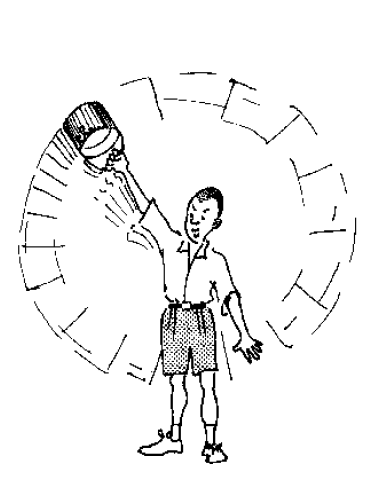
\includegraphics[width=0.45\textwidth]{./img/source/bucket-swing-2.png}
\end{center}

%\begin{description*}
%%\item[Subtopic:]{}
%\item[Materials:]{}
%\item[Setup:]{}
%\item[Procedure:]{}
%\item[Hazards:]{}
%\item[Questions:]{}
%\item[Observations:]{}
%\item[Theory:]{}
%\item[Applications:]{}
%\item[Notes:]{}
%\end{description*}

A bucket of water is sufficient to start investigating the effect of centripetal forces. Fill the
bucket with various quantities of water and you will learn even more by doing. Increase the
number of revolutions of the bucket.\\

Physics must not be a boring, tough subject, just good for exams and to be understood by a
few ``experts'' only. Physics should not happen in books only. It is everywhere where things
are. The teaching of science without experiments is just like a ngoma without dancers.\\

Pupils learn more and better by doing. Stimulate them to investigate their environment
through easy to carry out experiments. Ask the pupils to make a list of physical phenomena
which can be observed in their environment. Let the pupils enjoy physics. The activities in this book
show how this can be achieved.

\vfill
\columnbreak


%==================================================================================================%

\section*{Applications of Physics} \index{Physics! applications of}


\subsection{Measurement and Data} \index{Measurement! introduction}

\begin{center}
\includegraphics[width=0.4\textwidth]{./img/source/butcher.png}
\end{center}

Imagine you would buy different kinds and different quantities of meat. The butcher will have
to weigh and then calculate the price for each kind of meat and produce the total bill. Thus,
measuring and the collection of data happen everyday in our life.\\

The tailor takes the measurements of his customer and of the material needed for a suit. The
milkman measures the volume of the milk sold. The technician measures with a caliper the
diameter of a screw and even at school the time of each period is measured. Especially in
engineering precise measurements are indispensable.

\vfill
\columnbreak

\subsection{Mechanics} \index{Mechanics}

\begin{center}
\includegraphics[width=0.4\textwidth]{./img/source/mechanics.png}
\end{center}

Have you observed children balancing a plank like a seesaw? They know how a big and a
small child can balance although they are of different weight.\\

Usually they do not know what a fulcrum, a load distance and a moment of force is. However,
such basic mechanics dominate an essential part of our daily life. We encounter motion,
friction, inertia, work and power almost every day. We also learn in a practical way about
density, pressure of fluids or gases. Work, energy, power and other physical phenomena look
very abstract in books but happen every day. Also the movement of earth, moon and the
planets which determines the lengths of our days, months and years, has to do with basic
mechanics such as motion, mass attraction and centripetal forces.

\subsection{Matter} \index{Matter! introduction}

\begin{center}
\includegraphics[width=0.4\textwidth]{./img/source/matter.png}
\end{center}

A chair can be touched. Water in a bucket also. But air? Can you imagine that while you are
reading these lines your nose is punched more than 100 billion times by air molecules?\\

The environment around us, whether in solid, liquid or gaseous state is made up of billions of
tiny particles which are either molecules or atoms. These particles which constitute air are so
tiny, that we cannot see them even by a powerful microscope. However, the students can be
given an idea of the particle structure of matter by indirect evidence.

\subsection{Thermal Physics} \index{Thermal physics! introduction}

\begin{center}
\includegraphics[width=0.4\textwidth]{./img/source/thermal-physics.png}
\end{center}

Would you ever touch the handle of a hot pan? Would you put margarine just aside
of the pot? Would you hold your hand right above the hot water? No; this is
because we know a lot about thermal physics by daily experience. But we do not always
relate this knowledge with what we learn at school about heat conduction, heat radiation or
heat convection as is the case in the examples mentioned above.\\

Thermal physics has also to do with thermal energy and the measurement of temperatures,
with calorimetry, change of states, expansion, etc. Ask the students to talk about everyday
thermal phenomena and to write about these. Why should we teach this topic by talk and
chalk only, if there are illustrative experiments which do not require a lot of equipment and
which are not time consuming in their preparation and performance?

\subsection{Wave Motion} \index{Waves! introduction}

\begin{center}
\includegraphics[width=0.4\textwidth]{./img/source/wave-motion.jpg}
\end{center}

Communication through spoken words has to do with the transport of waves. Telephone and
radio are well known. But do we think about waves when we hear a music band, when a crow
is croaking or when children are playing with a string telephone? All this is everyday knowledge about the transport of sound waves.\\

But teaching about waves does not mean only sound waves. Water waves we notice in a puddle as well as in a cup of tea. Electromagnetic waves are responsible for hearing our radios and watching our televisions.
Produce waves in physics not only by talking. Meaningful and simple experiments are
possible on many themes of this topic. No time? Hand experiments are always brief,
illustrative and can be carried out with everyday things.

\subsection{Light and Optics} \index{Light! introduction}

\begin{center}
\includegraphics[width=0.4\textwidth]{./img/source/light-optics.png}
\end{center}

When we hear about optics, the optician, eye glasses and lenses come into our mind. But that
is not all what optics is about. Optics is also about the reflection of an image in a mirror or in a
water puddle. The water surface is like a mirror. The image to be seen is inverted and it
seems to be as far behind the water surface as the object is in front of it.\\

Perhaps there are no curved mirrors at your school to teach about concave and convex mirrors. No problem. Take a polished spherical spoon and you will be able to perform an interesting lesson. Certainly not all themes can be taught by simple qualitative hand experiments only. But you may be astonished to see how many there are for eye catching demonstrations.

\subsection{Electricity and Magnetism} \index{Electricity! introduction} \index{Magnetism! introduction}

\begin{center}
\includegraphics[width=0.4\textwidth]{./img/source/elec-mag.png}
\end{center}

Effects of electricity can be observed nowadays nearly everywhere. A light bulb lights the
room; a radio enchants our ears; a torch helps to find our way in the darkness; and last but
not least we do owe a cool soft drink to a refrigerator. The understanding on how electric
apparatus work is essential nowadays.\\

But electricity does not only mean a current flows in a circuit. It means also static electricity or lightning during a thunderstorm. The topic of electricity is closely related to magnetism.
Without magnets electric motors would not work. Loudspeakers work with magnets and even
a simple bicycle dynamo has one. In harbours you can see how ``attractive'' magnets can be
to lift heavy loads. Do you think that the teaching of electricity by doing is difficult, needs a lot
of equipment and is even dangerous? See that this is not the case by trying some of the activities provided in this manual.

%==================================================================================================%


\end{multicols}

\pagebreak
\section{Introduction to Laboratory Practice} 

\begin{multicols}{2}


%==================================================================================================%

\section*{Laboratory Rules and Safety} \index{Laboratory! rules and safety}


\subsection[Display of Hazardous Chemicals]{Display of Hazardous \hfill \\ Chemicals}

\begin{center}
\includegraphics[width=0.45\textwidth]{./img/source/display-chemicals.jpg}
\end{center}

\begin{description*}
%\item[Subtopic:]{}
%\item[Materials:]{}
%\item[Setup:]{}
\item[Procedure:]{Display some well labelled containers with
hazard symbols for the students and let them
talk about them.}
%\item[Hazards:]{}
%\item[Questions:]{}
%\item[Observations:]{}
%\item[Theory:]{}
%\item[Applications:]{}
%\item[Notes:]{}
\end{description*}

\subsection{A Safety Game}

\begin{center}
\includegraphics[width=0.45\textwidth]{./img/source/safety-game.jpg}
\end{center}

\begin{description*}
%\item[Subtopic:]{}
\item[Materials:]{Cards of hazard symbols}
%\item[Setup:]{}
\item[Procedure:]{Play a game with the symbol charts. A
student is given a hazard symbol. He has to
explain the hazard shown and to explain the
necessary safety precautions in order to avoid
that hazard.}
%\item[Hazards:]{}
%\item[Questions:]{}
%\item[Observations:]{}
%\item[Theory:]{}
%\item[Applications:]{}
%\item[Notes:]{}
\end{description*}

\columnbreak

\subsection{The Cleanliness Play}

\begin{center}
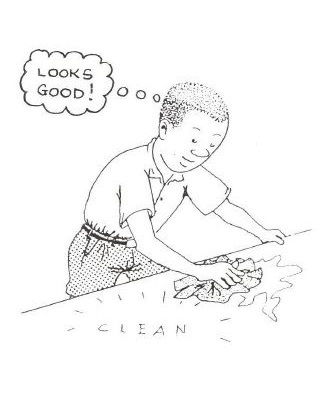
\includegraphics[width=0.45\textwidth]{./img/source/cleanliness-play.jpg}
\end{center}

\begin{description*}
%\item[Subtopic:]{}
%\item[Materials:]{}
%\item[Setup:]{}
\item[Procedure:]{Ask the students to play group-wise short
and funny scenes using appropriate words to
make them familiar with cleanliness rules.}
%\item[Hazards:]{}
%\item[Questions:]{}
%\item[Observations:]{}
%\item[Theory:]{}
%\item[Applications:]{}
%\item[Notes:]{}
\end{description*}

\subsection{The Tidiness Play}

\begin{center}
\includegraphics[width=0.45\textwidth]{./img/source/tidiness-play.jpg}
\end{center}

\begin{description*}
%\item[Subtopic:]{}
%\item[Materials:]{}
%\item[Setup:]{}
\item[Procedure:]{Chemists are very tidy. Apparatus and
reagents should be arranged on the table so that
they can be reached easily but at a safe distance
from the experiment.}
%\item[Hazards:]{}
%\item[Questions:]{}
%\item[Observations:]{}
%\item[Theory:]{}
%\item[Applications:]{}
%\item[Notes:]{}
\end{description*}

\end{multicols}

\pagebreak

%==================================================================================================%

\section*{The Scientific Method} \index{Scientific method}
\label{sec:scientific-method}

%\setcounter{secnumdepth}{1}

The following activities can be used as a method of introducing students to the scientific method. Rather than just performing the activities, first identify the question or problem with the students, then have them form a hypothesis for each step of the experiment. Students should record observations and data accordingly and use them to draw a conclusion about the activity.\\

Prepare an activity sheet for each student or have them copy it into their notebooks before performing the activities. Set up stations for the various activities and have students rotate among them in small groups. Incorporate activities in Biology and Chemistry as well from the \emph{Shika na Mikono} resource manual.\\


\subsection{Complete the Circuit} \index{Electricity! current}

\begin{center}
\includegraphics[width=0.8\textwidth]{./img/conductors-insulators-sci-meth.png}
\end{center}

\begin{description*}
\item[Materials:]{Dry cell, speaker wire, bulb/ammeter, cardboard, various objects, e.g. rubber band, nail, paper, aluminum foil, toothpick, pen, scissors, bottle cap, coin, balloon, chalk}
\item[Setup:]{Connect a dry cell and bulb in series using speaker wire and attach to a sheet of cardboard. Leave two wires free and pin to the cardboard to act as a switch.}
\item[Problem:]{Which objects will light a bulb?\\

\begin{tabular}{|l|c|c|} \hline
\multirow{2}{*}{\textbf{Object}} & \textbf{Hypothesis} & \multirow{2}{*}{\textbf{Experimental Result}} \\
& \textbf{(Light or No Light)} & \\ \hline
Copper wire & & \\ \hline
Pen & & \\ \hline
Aluminum foil& & \\ \hline
Paper& & \\ \hline
Nail& & \\ \hline
Toothpick& & \\ \hline
Bottle cap& & \\ \hline
Balloon& & \\ \hline
Chalk& & \\ \hline
Scissors (blade)& & \\ \hline
Scissors (handle)& & \\ \hline
\end{tabular}\\[10pt]
}
\item[Hypothesis:]{Predict which materials will cause the bulb to light when placed across the switch. Record predictions in the table.}
\item[Procedure:]{Test each object by placing it across the free wires to close the circuit.}
\item[Observations:]{Record the result for each item in the table.}
\item[Questions:]{}\hfill 
\begin{enumerate}
\item Which materials caused the bulb to light?
\item These objects are made from what kind or materials?
\item What other objects in the room can you find to test? Will they light the bulb?
\end{enumerate}
\item[Theory:]{\emph{Conductors} are materials which easily allow electrons to flow through them. \emph{Insulators} are materials which do not easily allow the the flow of electrons. Examples of good conductors are most metals, water and the human body. Examples of good insulators are rubber, wood and plastic.}
\end{description*}

\pagebreak


\subsection{Density Tower} \index{Density}

\begin{center}
\includegraphics[width=0.3\textwidth]{./img/density-tower-sci-meth.png}
\end{center}

\begin{description*}
\item[Materials:]{Syringes, bottles, water, cooking oil, kerosene, spirit, honey, glycerine, tape, scissors}
\item[Setup:]{Prepare a test tube rack by cutting a bottle and filling it with dirt. Remove the plungers from the syringes and seal them with tape, super glue, or by melting to opening closed.}\\
\item[Problem:]{Which liquids are more dense than others?\\

\begin{tabular}{|l|c|c|} \hline
\multirow{2}{*}{\textbf{Liquid}} & \textbf{Hypothesis} & \multirow{2}{*}{\textbf{Experimental Result}} \\
& \textbf{(Position, 1 = bottom)} & \\ \hline
Water & & \\ \hline
Cooking oil & & \\ \hline
Kerosene & & \\ \hline
Spirit & & \\ \hline
Honey & & \\ \hline
Glycerine & & \\ \hline
\end{tabular} \\[10pt]
}\\
\item[Hypothesis:]{Predict the order in which the liquids will settle from the bottom of the syringe. Assign 1 to the bottom liquid, 2 to the one above it, and so on.}
\item[Procedure:]{Pour a small amount of each liquid into a syringe, observing after each addition.}
\item[Observations:]{After adding all liquids, record the order in which they rest, starting with 1 at the bottom.}
\item[Questions:]{}\hfill
\begin{enumerate}
\item Which liquid finished at the bottom?
\item Which liquid finished at the top?
\item Which liquid has the greatest density?
\item Which liquid has the lowest density?
\item What happens if you place a small object (e.g. paper clip, eraser, paper) in the tower? 
\end{enumerate}
\item[Theory:]{\emph{Density} is a property of different materials and liquids. It is a ratio of its mass to its volume. Dense liquids sink to the bottom, while less dense liquids rise to the top. A small object placed in the tower will settle in the liquid which is nearest its own density.}
\end{description*}

\pagebreak


\subsection{Sinkers and Floaters} \index{Flotation}

%\begin{center}
%\includegraphics[width=0.4\textwidth]{./img/source/.jpg}
%\end{center}

\begin{description*}
\item[Materials:]{Basin of water, various objects, e.g. nail, paper clip, paper, aluminum foil, soda cap, matchbox, pen cap, toothpick, balloons, flour}
%\item[Setup:]{}\\
\item[Problem:]{Which objects sink or float when placed in water?\\

\begin{tabular}{|l|c|c|} \hline
\multirow{2}{*}{\textbf{Object}} & \textbf{Hypothesis} & \multirow{2}{*}{\textbf{Experimental Result}} \\
& \textbf{(Sink or Float)} & \\ \hline
Nail& & \\ \hline
Paper clip& & \\ \hline
Pen cap& & \\ \hline
Soda cap (dropped)& & \\ \hline
Soda cap (placed carefully)& & \\ \hline
Toothpick & & \\ \hline
Paper& & \\ \hline
Aluminum foil& & \\ \hline
Matchbox& & \\ \hline
Balloon (empty)& & \\ \hline
Balloon (filled with flour)& & \\ \hline
Balloon (filled with water)& & \\ \hline
Balloon (filled with air)& & \\ \hline
\end{tabular} \\[10pt]
}\\
\item[Hypothesis:]{Predict whether each object will sink or float when placed in the basin of water. Record in the table.}
\item[Procedure:]{Place each object in the water. First place them very carefully, then drop them in.}
\item[Observations:]{Record the results in the table.}
\item[Questions:]{}\hfill
\begin{enumerate}
\item What factors affect whether an object sinks or floats?
\item How do large objects such as boats float?
\end{enumerate}
\item[Theory:]{\emph{Flotation} depends on several things. A bottle cap placed carefully on the surface of the water will float, but when pushed under, will sink. A sheet of aluminum foil will float while a sheet of the same size which is folded several times will sink. A balloon filled with flour sinks, one filled with water just floats, and one filled with air floats above the surface.\\

If an object's \emph{total density} is greater than that of water, it sinks, but if less than water, it floats. Air has a density less than water, so when air is trapped in objects such as bottle caps or balloons, they float because their total density is less than water. When air is removed (folded aluminum foil) or replaced by water (bottle cap), the total density of the object is just the density of the material. A matchbox pushed under water rises back to the surface because its density is less than that of water.\\

Boats are able to float despite being built from dense materials because of the large volume of water they displace and the large amount of air inside the boat. A boat with a larger surface area displaces a larger volume of water and thus can carry a larger load before sinking.\\

Follow up this activity with the \emph{Raft Rally} science competition.}
\end{description*}

\pagebreak


\subsection{Mixing Colours} \index{Colour}

%\begin{center}
%\includegraphics[width=0.4\textwidth]{./img/source/.jpg}
%\end{center}

\begin{description*}
\item[Materials:]{Various food colours, syringes, bottle, scissors, tape, paper}
\item[Setup:]{Prepare a test tube rack by cutting a bottle and filling it with dirt. Remove the plungers from the syringes and seal them with tape, super glue, or by melting to opening closed.}\\
\item[Problem:]{What happens when we mix different colours?\\

\begin{tabular}{|l|c|c|} \hline
\multirow{2}{*}{\textbf{Colours to Mix}} & \textbf{Hypothesis} & \multirow{2}{*}{\textbf{Experimental Result}} \\
& \textbf{(What colour?)} & \\ \hline
Red and green & & \\ \hline
Yellow and blue & & \\ \hline
Red and yellow & & \\ \hline
All colours & & \\ \hline
\end{tabular} \\[10pt]
}\\
\item[Hypothesis:]{Predict which colour will result when the two colours given are mixed together. Record it in the table.}
\item[Procedure:]{Use syringes to remove small amounts of each colour and place on a sheet of paper. Be sure to lay down plenty of paper so that the colours do not bleed through onto the table!}
\item[Observations:]{Record the resulting colour mixture in the table.}
\item[Questions:]{}\hfill
\begin{enumerate}
\item How can you make orange from other colours?
\item What colour do you get by mixing all of the colours together?
\item What are some uses of coloured dyes?
\end{enumerate}
\item[Theory:]{Red, green and blue are \emph{primary colours} of light. Other colours are made by different combinations of these primary colours. Coloured dyes are used for many applications, including clothes, paper and printing pictures.}
\end{description*}

%==================================================================================================%

%\setcounter{secnumdepth}{2}

%\end{multicols}
\vfill
\pagebreak
\section{Measurement and Density/Relative Density} \index{Measurement}

Human progress is due, in large part, to an ability to measure and hence collect data with
greater and greater precision. Young students should learn, generally, about how to obtain data
by carrying out simple experiments. They should be introduced to the basic measurements of
mass, distance and time. They should be trained in recording and in graphical analysis of
data.

\begin{multicols}{2}

\section*{Collection of Data} \index{Data collection}


\subsection{Data on Weighing} \index{Elasticity}

\begin{center}
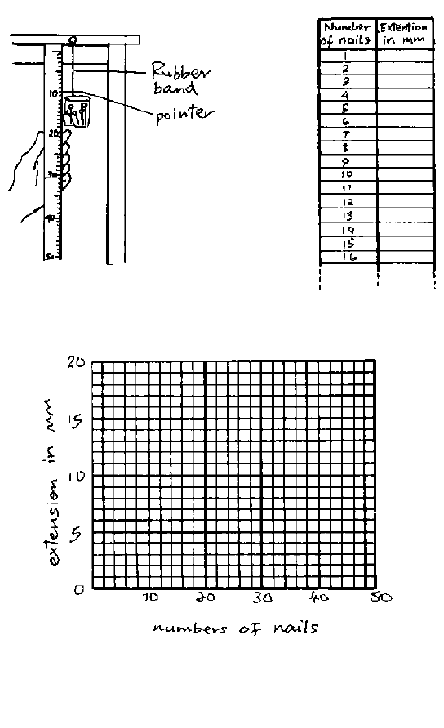
\includegraphics[width=0.5\textwidth]{./img/source/meas-mass.png}
\end{center}

Fix a rubber band at one end to a table or retort stand. At the other end, attach a paper clip to act as a pointer and a small bag or scale pan. Fill the bag or scale pan with successive numbers of nails. Have students measure the extension of the rubber band each time they add more nails. Record the readings and use the data to draw a graph as shown in the figure.

\vfill
\columnbreak

\subsection{Data on Distance}

\begin{center}
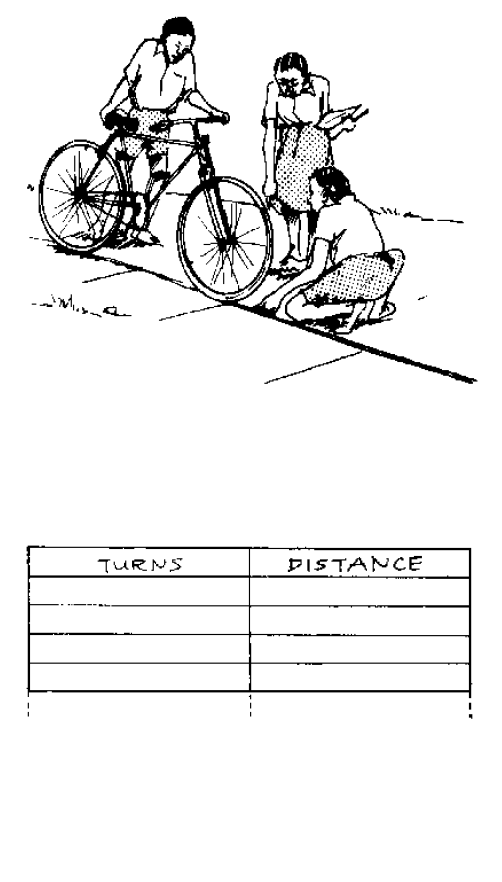
\includegraphics[width=0.5\textwidth]{./img/source/meas-distance.png}
\end{center}

Make a mark on the tyre of a bicycle at the point where it touches the ground. Turn the tyre by moving the bicycle forward and record the length of one turn. Repeat the experiment several times for various numbers of turns, each time recording the horizontal distance covered. Draw a graph to show the data.

\vfill
\columnbreak

\subsection{Data on Time} \index{Pendulum! simple}

\begin{center}
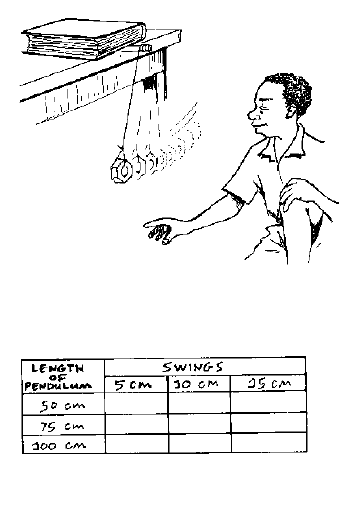
\includegraphics[width=0.5\textwidth]{./img/source/meas-time.png}
\end{center}

Fix a string just off the edge of a table and hang a small weight (e.g. a nut or nail) at a distance of 50 cm. This is a simple pendulum. Pull the pendulum to one side so that its horizontal displacement is 5 cm. Count the number of oscillations (back and forth) made in one minute. Repeat by increasing the horizontal displacement to 10 cm and 15 cm. Then try varying the length of the string. How long must the pendulum be to oscillate 60 times in one minute?

\vfill
\columnbreak

\subsection{Data on Velocity}

\begin{center}
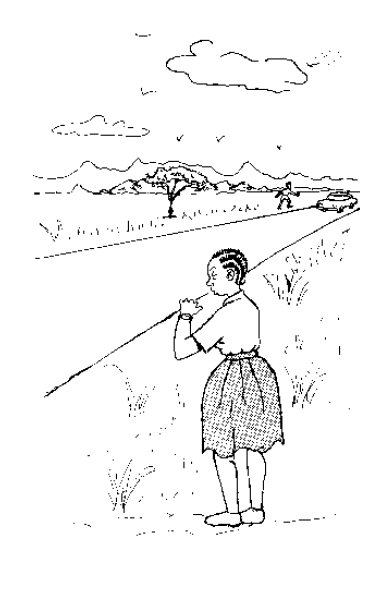
\includegraphics[width=0.5\textwidth]{./img/source/meas-velocity.png}
\end{center}

Mark a distance of 100 metres along a nearby road or playground. Note the time taken for a
car, a bicycle or a sprinter to cover the distance as follows. One pupil waves down his hand
as either the car, bicycle or sprinter crosses the 0 metres mark. Another pupil with a watch,
starts timing at the same time. A third pupil at the 100 metre mark waves down his hand as
the moving object crosses the 100 metre mark and at this instant the timekeeper stops his
watch.

\vfill
\columnbreak

%\subsection{Mass vs. Weight}

%==================================================================================================%

\section*{Measuring Instruments}


\subsection{Construction of a Metre Rule} \index{Metre rule}
\label{sub:metrerule}

\begin{description*}
%\item[Subtopic:]{Concept of Measurement}
\item[Materials:]{Wooden board, pen\slash pencil, a handsaw, ruler or tape measure}
%\item[Setup:]{}
\item[Procedure:]{Use the handsaw to cut a piece of wood 100 cm $\times$ 3.5 cm $\times$ 0.5 cm. Use a ruler or tape measure to mark a scale in cm on the wood.}
%\item[Hazards:]{}
%\item[Questions:]{}
%\item[Observations:]{}
%\item[Theory:]{}
\item[Applications:]{Students can record data on their height, dimensions of the classroom, etc.}
\item[Notes:]{Instead of a wooden block, string can be used by making knots at different intervals.}
\end{description*}

\subsection[Construction of a Beam Balance]{Construction of a Beam \hfill \\ Balance} \index{Beam balance}
\label{sub:beambalance}

\begin{center}
\includegraphics[width=0.5\textwidth]{./img/beam-balance.png}
%\includegraphics[width=0.4\textwidth]{./img/source/simple-balances.png}
\end{center}

\begin{description*}
%\item[Subtopic:]{Concept of Measurement}
\item[Materials:]{Ruler or wooden bar 30 cm $\times$ 2 cm, nails, razor/knife, string/wire, pen, 2 \nameref{sub:scalepans}}
%\item[Setup:]{}
\item[Procedure:]{Find the balancing point of the ruler and mark it with a pen. Use a heated nail to make a hole through this point. Make notches at 5 cm intervals on either side of the center hole using a razor/knife to suspend scale pans. Suspend the balance with a string/wire.}
%\item[Hazards:]{}
%\item[Questions:]{}
%\item[Observations:]{}
%\item[Theory:]{}
%\item[Applications:]{Principle of Moments}
\item[Notes:]{Use locally available \nameref{sec:masses} to find the mass of everyday objects, e.g. notebooks, pens, rulers.}
\end{description*}

\columnbreak

\subsection{Scale Pans} \index{Scale pans}
\label{sub:scalepans}

\begin{center}
\includegraphics[width=0.4\textwidth]{./img/source/scale-pans.png}
\end{center}

\begin{description*}
%\item[Subtopic:]{Concept of Measurement}
\item[Materials:]{Match boxes, large plastic bottles, tin can lids, small plastic bags, knife, string}
%\item[Setup:]{}
\item[Procedure:]{Use a knife to poke 3~-~4 holes in the sides of one of the above materials. If using plastic bottles, cut them about 3~-~4~cm from the bottom. Cut equal lengths of string and tie them through the holes in the scale pan. Join the strings together at the upper end. }
%\item[Hazards:]{}
%\item[Questions:]{}
%\item[Observations:]{}
%\item[Theory:]{}
%\item[Applications:]{}
%\item[Notes:]{}
\end{description*}

\subsection{Construction of a Measuring Cylinder} \index{Measuring cylinder}
\label{sub:meascyl}

%\begin{center}
%\includegraphics[width=0.2\textwidth]{./img/vso/meas-cyl.jpg}
%\end{center}

\begin{description*}
%\item[Subtopic:]{Concept of Measurement}
\item[Materials:]{Plastic bottles of different sizes, syringes (10 mL - 50 mL), marker pen, ruler, bucket of water}
%\item[Setup:]{}
\item[Procedure:]{Using the syringe, transfer a known volume of water from the bucket to the empty bottle. Use the marker pen to mark the level of water on the bottle. Repeat for a range of volumes, using a ruler to complete the scale.}
%\item[Hazards:]{}
%\item[Questions:]{}
%\item[Observations:]{}
%\item[Theory:]{}
%\item[Applications:]{}
%\item[Notes:]{}
\end{description*}

\subsection{Construction of a Eureka Can} \index{Eureka can}
\label{sub:eurekacan}

\begin{center}
\includegraphics[width=0.3\textwidth]{./img/vso/overflow-can.jpg}
\end{center}

\begin{description*}
%\item[Subtopic:]{Determining the Volume of Irregular Objects}
\item[Materials:]{Plastic bottle, knife}
%\item[Setup:]{}
\item[Procedure:]{Cut a plastic bottle about 10~cm from the bottom. Cut 2 slits at the top of the bottle and bend the strip forward to form a spout.}
%\item[Hazards:]{}
%\item[Questions:]{}
%\item[Observations:]{}
%\item[Theory:]{}
\item[Applications:]{Measuring the volume of irregular objects, Archimedes' Principle}
\item[Notes:]{Alternatively, use a bottle or tin can and poke a hole near the top using a heated nail. Attach a straw/hollow pen tube/tube of aluminum foil, using super glue to ensure an air-tight seal.}
\end{description*}

\columnbreak

\subsection{Errors in Measurement} \index{Measurement! errors}
\label{sub:meas-errors}

\begin{description*}
%\item[Subtopic:]{}
\item[Materials:]{Metre rules, stopwatches}
%\item[Setup:]{}
\item[Procedure:]{(a) Draw a line on the board or floor. Have several students measure the length and secretly record their results. Collect the results and record them on the board, noting any differences.\\(b) Distribute stopwatches to several students. Clap twice and have students measure the time betweeen claps and secretly record their results. Collect the results and record them on the board, observing any differences.}
%\item[Hazards:]{}
\item[Questions:]{What is the best result to use for each of the collected measurements?}
%\item[Observations:]{}
\item[Theory:]{Measurements vary from person to person. Every measurement comes with some level of error, and so it is important to take care when measuring to increase accuracy. The best result to use is the average of all the measurements.}
%\item[Applications:]{}
%\item[Notes:]{}
\end{description*}

%==================================================================================================%

\section*{Density/Relative Density} \index{Density|textbf} \index{Relative density|see{Density}|textbf}

%Density can be found by taking the ratio of a body's mass to its volume. Common units of density are g/mL and kg/L. $$ \mathrm{Density} = \mathrm{mass} \div \mathrm{Volume} $$$$ \rho = \cfrac{m}{V} $$
%Relative density (R.D.) can be used to compare the density of a given material to that of water.  Water is the standard with a density of 1.0 g/cm$^3$ (or 1 000 kg/m$^3$), so all other densities are compared to water. Because relative density is a ratio of two densities, it has no units.
%$$\mathrm{R.D.} = \frac{\mathrm{Density\; \; of \;substance}}{\mathrm{Density\; \;of \;water}}$$


%\subsection{Density of a Solid}

\subsection{Density Tower}
\label{sub:density-column}

\begin{center}
\includegraphics[width=0.3\textwidth]{./img/density-tower.png}
\end{center}

\begin{description*}
%\item[Subtopic:]{}
\item[Materials:]{Syringes, water, honey, glycerine, cooking oil, spirit, kerosene, erasers, paper clips, nails, other small objects}
%\item[Setup:]{}
\item[Procedure:]{Add each liquid into the syringe, one by one, observing the relative depths of each liquid. Place small solid objects e.g. rubber erasers, paper clips, small nails, etc. into the syringe and observe their positions relative to the various liquids.}
%\item[Hazards:]{}
\item[Questions:]{Which liquid is the most dense? Which is the least dense?}
\item[Observations:]{The denser liquids sink to the bottom while the less dense liquids rise to the top. The solid objects settle among liquids of comparable density.}
%\item[Theory:]{$ \mathrm{Density} = \mathrm{mass} \div \mathrm{Volume} $ ($ \rho = \cfrac{m}{V} $). Relative density (R.D.) can be used to compare the density of a given material to that of water. Liquids with a greater density sink to the bottom, while those having a lower density rise to the top.}
\item[Applications:]{Relative densities of liquids and solids help to identify certain substances, e.g. whether a ring is really made of gold.}
\item[Notes:]{Food coloring can be added to colorless liquids such as water, kerosene and glycerine to help distinguish among them.}
\end{description*}

%\subsection{Relative Density of a Liquid}

\subsection{U-Tube Apparatus}
\label{sub:u-tube}

\begin{description*}
%\item[Subtopic:]{}
\item[Materials:]{3 clear plastic pen tubes, cardboard, heated nail or knife, tape, pen, super glue, water, kerosene.}
\item[Setup:]{Cut two of the tubes at one end to make a 45$^\circ$ angle, and cut the third tube (shorter than the other two) to make a 45$^\circ$ angle at both ends. Attach the two longer tubes to either side of the short one so that they make right angles and form a U-shape. Melt the angled ends together with a hot knife, soldering iron, etc. so that the apparatus is water-tight. Glue the assembly to a cardboard base so that it stands upright. 

Place thin strips of tape along each side of the U-tube and mark with identical scales. Do this by adding known volumes of water and marking the levels on each scale. Label these marks from top to bottom as 0, 1, 2, etc.}
\item[Procedure:]{Place an amount of water into the U-tube such that the water rises about half way on either side of the tube. The actual volume of water is not important as long as you can see the levels clearly. Stand the tube upright and slowly drip about 1 mL of kerosene into one side of the U-tube. Measure the relative heights of water and the kerosene from the bottom level of the kerosene.}
%\item[Hazards:]{}
%\item[Questions:]{}
\item[Observations:]{The kerosene will displace the water, so you should see the water level on the other side rise slightly.}
\item[Theory:]{If a fluid’s density is less than that of water, it will float on top, displacing the water on the other side of the tube. From Archimedes’ principle and the Law of Flotation, we know that \[ \frac{\text{height of water}}{\text{height of kerosene}} = \frac{\text{density of kerosene}}{\text{density of water}} \]. The scales drawn on the outside of the U-tube allow us to find the ratio of the heights without needing units, and the density of water is known to be 1.0 g/mL, so the density of the other fluid can be calculated.}
%\item[Applications:]{}
\item[Notes:]{If the other fluid has a higher density than water, the experiment can still be done, but the fluid with higher density must be added first, then displaced with water, performing the same calculation.}
\end{description*}

\end{multicols}

\pagebreak
\section{Force} \index{Forces}

\begin{multicols}{2}

\section*{Concept of Force}


\subsection{Examples of Forces}
\begin{center}
\includegraphics[width=0.5\textwidth]{./img/vso/forces-ex.jpg}
\end{center}

A \textbf{force} is any push or pull on an object. Examples of forces in our daily life include kicking a football, walking due to friction, hammering a nail and dropping an object. What other examples can you think of?

\subsection{Making a Spring Balance} \index{Spring balance}

\begin{center}
\includegraphics[width=0.26\textwidth]{./img/source/spring-balance.png}
\end{center}

\begin{description*}
%\item[Subtopic:]{Concept of Force}
%\item[Shika Rating:]{4}
\item[Materials:]{Cardboard, strong rubber band, staple pin, 2 paper clips, \nameref{sec:masses}}
\item[Setup:]{Take a strip of cardboard or wood and fix a strong rubber band to it using a staple pin. (The stronger the rubber band, the larger the force you can measure.) Attach one paper clip as a pointer as shown in the figure. Then fix another as a hook at the bottom end of the rubber band.}
\item[Procedure:]{Calibrate the balance in \emph{Newtons} using either a standard set of \nameref{sec:masses} or another spring balance. A mass of 10 g has a weight of 0.1 N; a mass of 100 g has a weight of 1 N, etc. Draw marks accordingly on the scale of the balance.}
\item[Hazards:]{Never apply such a large force that the pointer does not return to the zero mark when the force ceases.}
%\item[Questions:]{}
%\item[Theory:]{}
\item[Applications:]{Use the spring balance to measure the weight of small objects or the force of pulling an object along a table.}
%\item[Notes:]{}
\end{description*}

%==================================================================================================%

\section*{Effects of Forces}
%Forces can have a variety of effects on objects, including \emph{stretching}, \emph{compression} (or \emph{restoring}), \emph{attraction}, \emph{repulsion}, \emph{torsion}, \emph{friction}, \emph{viscosity} and \emph{air resistance}. These effects are seen all around us in our daily lives.


\subsection{Observing Effects of Forces}

\begin{center}
\includegraphics[width=0.45\textwidth]{./img/source/effects-forces.png}
\end{center}

\begin{description*}
%\item[Subtopic:]{}
\item[Materials:]{Rubber bands, springs, magnets, ruler, honey, water, paper}
%\item[Setup:]{}
\item[Procedure:]{Have students investigate different effects of forces using common materials.}
%\item[Hazards:]{}
%\item[Questions:]{}
\item[Observations:]{Rubber bands and springs stretch when pulled and then restore their shape. Magnets attract and repel each other. A ruler can be twisted under torsion. Rubbing hands together produces heat from friction. Honey pours more slowly than water due to a higher viscosity. A sheet of paper falls to the ground slowly because of air resistance.}
%\item[Theory:]{}
\item[Applications:]{Brainstorm various applications of the effects of forces with the class.}
%\item[Notes:]{}
\end{description*}

\subsection{Presence of Gravity} \index{Gravity! presence of}
\begin{description*}
%\item[Subtopic:]{}
\item[Materials:]{Pen, ruler, sheet of paper, book (same size as paper)}
%\item[Setup:]{}
\item[Procedure:]{Drop the pen and ruler side by side from shoulder height. Repeat with a pen and sheet of paper. Then place the paper on top of a book and drop side by side with a regular sheet of paper. Bunch the paper into a tight ball and drop it again with the book.}
%\item[Hazards:]{}
\item[Questions:]{Which objects fell at the same rate? Which ones fell more slowly?}
\item[Observations:]{All objects, with the exception of paper and other light, wide objects, fall at exactly the same rate.}
\item[Theory:]{Gravity pulls on all objects on earth the same.  The paper falls slowly because it is more affected by air resistance due to its small weight and large surface area. Placing a book under the paper reduces air resistance by blocking all of the air which would normally push against the paper. Thus they fall at the same rate.  When the paper is bunched into a ball, the mass stays the same but the air resistance is greatly reduced so it falls at the same rate as the book.}
%\item[Applications:]{}
%\item[Notes:]{}
\end{description*}

\subsection{Helicopters} \index{Helicopters}

\begin{center}
\includegraphics[width=0.4\textwidth]{./img/helicopter-1.png}
\end{center}

\begin{center}
\includegraphics[width=0.4\textwidth]{./img/helicopter-2.png}
\end{center}

\begin{description*}
%\item[Subtopic:]{}
\item[Materials:]{Paper, scissors, paper clip}
%\item[Setup:]{}
\item[Procedure:]{Copy the following design onto a piece of paper. Cut along the solid lines and fold along the dotted lines, attaching the paper clip to the bottom. Drop the helicopter with the paperclip down and watch it spin!}
%\item[Hazards:]{}
\item[Questions:]{Does the helicopter spin more if you add more paper clips? If you change the size/number of wings?}
\item[Observations:]{Adding more paper clips causes the helicopter to spin faster. Increasing the surface area of the wings also increases the rate of spin.}
\item[Theory:]{The helicopter spins because the force of air resistance pushing up on the wings creates a moment about the vertical axis of rotation. Increasing the force of air resistance increases this moment and the helicopter spins faster.}
%\item[Applications:]{}
%\item[Notes:]{}
\end{description*}

\subsection{Forces on Bridges}

\begin{center}
\includegraphics[width=0.5\textwidth]{./img/vso/forces-bridges.jpg}
\end{center}

\begin{description*}
%\item[Subtopic:]{}
%\item[Materials:]{}
%\item[Setup:]{}
%\item[Procedure:]{}
%\item[Hazards:]{}
%\item[Questions:]{}
%\item[Observations:]{}
\item[Theory:]{The bridge bends under the
weight of the load. More than
one force is at work. Compression
forces are concentrated on the
top surface. When a bridge
bends, compression on top
creates tension forces on the
bottom surface.}
%\item[Applications:]{}
%\item[Notes:]{}
\end{description*}

\subsection{Parachutes} \index{Parachutes}

\begin{center}
\includegraphics[width=0.4\textwidth]{./img/vso/parachute.jpg}
\end{center}

\begin{description*}
%\item[Subtopic:]{}
\item[Materials:]{Paper/newspaper/plastic bags, string, paper clips}
\item[Setup:]{Tie pieces of string (about 30 cm) to each corner of the paper/bag. Join the four strings together and attach a paper clip or other small weight.}
\item[Procedure:]{Drop the parachute side by side with a normal paper clip.}
%\item[Hazards:]{}
\item[Questions:]{Which one reaches the ground first? If the paper clip were a person, which one would arrive safely to the ground? Does a person using a parachute want to make it as large as possible or as small as possible?}
\item[Observations:]{The parachute falls more slowly because there is a larger space for air to enter and counteract the force of gravity pulling it to the ground.}
%\item[Theory:]{}
\item[Applications:]{Skydivers, military personnel, air-dropped aid packages. Follow up this activity with the \emph{Egg Drop} or \emph{Drop Zone} science competitions (see \emph{Shika na Mikono} resource manual).}
%\nameref{sec:drop-zone} or \nameref{sec:egg-drop} science competitions (p.~\pageref{ec:egg-drop}).}
\item[Notes:]{Poke a small hole in the top of the parachute and ask students what will happen.}
\end{description*}

\subsection{Strengthening Bridges}

\begin{center}
\includegraphics[width=0.4\textwidth]{./img/vso/strengthening-bridges.jpg}
\end{center}

\begin{description*}
%\item[Subtopic:]{}
\item[Materials:]{Books, string, nails, board}
%\item[Setup:]{}
\item[Procedure:]{Ask students to build the 2
bridges shown. Discuss why the
suspension bridge is stronger.}
%\item[Hazards:]{}
%\item[Questions:]{}
%\item[Observations:]{}
\item[Theory:]{In a suspension bridge the tension
in the bridge is increased by
securing the `strings' and
suspending them over towers or
from trees.}
\item[Applications:]{Follow up the discussion by having students compete in the \emph{Bridge Challenge} science competition (see \emph{Shika na Mikono} resource manual).}
%\nameref{sec:bridge-challenge} science competition (p.~\pageref{sec:bridge-challenge}).}
%\item[Notes:]{}
\end{description*}


\end{multicols}

\pagebreak
\section{Archimedes' Principle and the Law of Flotation} \index{Archimedes' principle} 

\begin{multicols}{2}


\section*{Concept of Upthrust}
\textbf{Archimedes' Principle} states that any object partially or totally immersed in a fluid experiences an upthrust equal to the weight of the fluid displaced by the body.
$$ \text{Upthrust} = \text{Weight of displaced fluid}$$
%$$ \text{Weight in air} - \text{Apparent weight in fluid} = \text{Weight of displaced fluid}$$

\subsection{Verifying Archimedes' Principle}

\begin{center}
\includegraphics[width=0.4\textwidth]{./img/source/upthrust.png}
\end{center}

\begin{description*}
%\item[Subtopic:]{}
\item[Materials:]{\nameref{sec:spring-balance}, stone, string, \nameref{sec:meascyl}, water, \nameref{sec:eureka-can}, syringe}
%\item[Setup:]{}
\item[Procedure:]{Tie a string around a stone and measure its weight in Newtons using a spring balance. Fill the measuring cylinder partially with water and record the reading. Immerse the stone fully into the water (without touching the bottom) and record the reading on the spring balance, as well as the new water level of the measuring cylinder.}
%\item[Hazards:]{}
\item[Questions:]{What is the change in weight of the stone as read from the spring balance? What is the weight of the displaced water (1 mL = 0.01 N)?}
%\item[Observations:]{}
\item[Theory:]{The change in weight of the stone is known as its \emph{Apparent Loss in Weight}, which is equal to the \emph{Upthrust} exerted on the stone by the water. Archimedes' Principle tells us that this is equal to the weight of the water displaced by the stone.}
%\item[Applications:]{}
\item[Notes:]{A Eureka can and syringe may be used to measure the displaced fluid in place of a measuring cylinder.}
\end{description*}

%==================================================================================================%

\section*{Sinking and Floating} \index{Flotation|textbf}
If the density of an object is less than that of the surrounding fluid, the object will float. If the density is greater than that of the fluid, it will sink.

\textbf{The Law of Flotation} states that a floating body displaces its own weight of the fluid in which it floats.
$$\text{Weight of body} = \text{Weight of displaced fluid}$$


\subsection{Verifying the Law of Flotation}

\begin{center}
\includegraphics[width=0.4\textwidth]{./img/source/flotation.png}
\end{center}

\begin{description*}
%\item[Subtopic:]{}
\item[Materials:]{\nameref{sec:spring-balance}, matchbox, stone, string, \nameref{sec:eureka-can}, \nameref{sec:meascyl}/syringe}
%\item[Setup:]{}
\item[Procedure:]{Load a matchbox with a small stone so that it still floats in water. Record the weight of the matchbox and stone in Newtons using a spring balance. Fill the Eureka can with water and allow the matchbox to float on it. Collect the overflow in a measuring cylinder or syringe. Calculate the weight of the overflow (1 mL = 0.01 N).}
%\item[Hazards:]{}
\item[Questions:]{How does the weight of the matchbox and stone compare to that of the displaced water?}
\item[Observations:]{The values should be equal, thus verifying the Law of Flotation.}
%\item[Theory:]{}
\item[Applications:]{Submarine, hot air balloon, ships. Design and selection of materials for these vessels are done using the Law of Flotation.}
%\item[Notes:]{}
\end{description*}

\vfill
\columnbreak

\subsection{Sinkers and Floaters}

%\begin{center}
%\includegraphics[width=0.4\textwidth]{./img/.jpg}
%\end{center}

\begin{description*}
%\item[Subtopic:]{}
\item[Materials:]{Basin of water, various objects, e.g. nail, paper clip, paper, aluminum foil, soda cap, matchbox, pen cap, toothpick, balloons, flour}
\item[Setup:]{Fill one balloon with flour, one with water, and one with air. They should all be the same size.}
\item[Procedure:]{Have students predict the outcome for each object. Then place each object in the water, first by placing very carefully, then by dropping it in.}
\end{description*}

\begin{tabular}{|l|c|} \hline
\textbf{Object} & \textbf{Sink or Float?} \\ \hline
Nail&  \\ \hline
Paper clip&  \\ \hline
Pen cap&  \\ \hline
Soda cap &  \\ \hline
Toothpick &  \\ \hline
Paper&  \\ \hline
Aluminum foil&  \\ \hline
Matchbox&  \\ \hline
Balloon (empty)&  \\ \hline
Balloon (flour)&  \\ \hline
Balloon (water)&  \\ \hline
Balloon (air)&  \\ \hline
\end{tabular} \\[10pt]
%\item[Hazards:]{}
\begin{description*}
\item[Questions:]{}\hfill
\begin{enumerate}
\item What factors affect whether an object sinks or floats?
\item How do large objects such as boats float?
\end{enumerate}
\item[Observations:]{A bottle cap placed carefully on the surface of the water will float, but when pushed under, will sink. A sheet of aluminum foil will float while a sheet of the same size which is folded several times will sink. A balloon filled with flour sinks, one filled with water just floats, and one filled with air floats above the surface.}
\item[Theory:]{If an object's \emph{total density} is greater than that of water, it sinks, but if less than water, it floats. Air has a density less than water, so when air is trapped in objects such as bottle caps or balloons, they float because their total density is less than water. When air is removed (folded aluminum foil) or replaced by water (bottle cap), the total density of the object is just the density of the material. A matchbox pushed under water rises back to the surface because its density is less than that of water.

%Boats are able to float despite being built from dense materials because of the large volume of water they displace and the large amount of air inside the boat. A boat with a larger surface area displaces a larger volume of water and thus can carry a larger load before sinking.
}
\item[Applications:]{See the section on \nameref{sec:scientific-method} (p.~\pageref{sec:scientific-method}) to conduct this activity as an experiment with students. Follow up this activity with the \emph{Raft Rally} science competition (see \emph{Shika na Mikono} resource manual).}
%\item[Notes:]{}
\end{description*}

\subsection{Egg Float}

\begin{center}
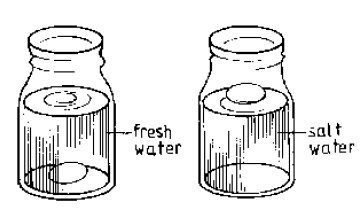
\includegraphics[width=0.49\textwidth]{./img/source/egg-float.png}
\end{center}

\begin{description*}
%\item[Subtopic:]{}
\item[Materials:]{2 fresh eggs, 2 containers (bottles cut in half), salt (less than half a cup)}
\item[Setup:]{Fill the two containers with water and place a fresh egg in each.}
\item[Procedure:]{Leave one as it is and add salt to the other. Add and mix salt until the egg floats in the saltwater container.}
%\item[Hazards:]{}
\item[Questions:]{Why does the egg float in saltwater but sink in fresh water?}
%\item[Observations:]{}
\item[Theory:]{Saltwater has a greater density than fresh water. A fresh egg has a density between fresh water and saltwater. Since an egg is denser than freshwater, it sinks. Since an egg is less dense than saltwater, it floats.}
\item[Applications:]{This is the same reason why it is easier to stay afloat when swimming in the ocean (saltwater) as opposed to a lake (fresh water).}
%\item[Notes:]{}
\end{description*}

\subsection{Floating Candle}

\begin{center}
\includegraphics[width=0.45\textwidth]{./img/source/floating-candle.png}
\end{center}

\begin{description*}
%\item[Subtopic:]{}
\item[Materials:]{Candle, nail, container, water}
%\item[Setup:]{}
\item[Procedure:]{Put a nail into the bottom end of a candle so that the candle just floats with its top a bit above the surface of the water. Light the candle and watch as it burns up.}
%\item[Hazards:]{}
\item[Questions:]{Why does the candle continue to float even though it loses weight as it burns up?}
%\item[Observations:]{}
\item[Theory:]{The candle continues to float because its density remains less than that of the surrounding water.}
%\item[Applications:]{}
%\item[Notes:]{}
\end{description*}

\vfill

\subsection{Cartesian Diver}

\begin{center}
\includegraphics[width=0.3\textwidth]{./img/cartesian-diver.png}
\end{center}

\begin{description*}
%\item[Subtopic:]{}
\item[Materials:]{1.5 L plastic bottle, balloon, paper clips (large), water}
\item[Setup:]{Fill the bottle with water. Fix a large paper clip to the lip of a balloon. Making sure to keep all air out of the balloon, insert it into the bottle. It should just float at the top while remaining completely submerged. Adjust depending on type of balloon and paper clips.}
\item[Procedure:]{Screw the cap on the bottle and squeeze the middle of the bottle, then release.}
%\item[Hazards:]{}
%\item[Questions:]{}
\item[Observations:]{The balloon should begin to sink when you squeeze, but float again when you release.}
\item[Theory:]{While water is nearly incompressible, the balloon (and any small amount of air inside) is compressible. This means when you squeeze the bottle, the water remains unchanged, but the balloon is compressed, decreasing its volume and so increasing its density. Before squeezing, it was less dense than the water and so it floated. After squeezing, it becomes denser than the water and sinks.}
%\item[Applications:]{}
%\item[Notes:]{}
\end{description*}

\subsection{The Hydrometer} \index{Hydrometer}

\begin{center}
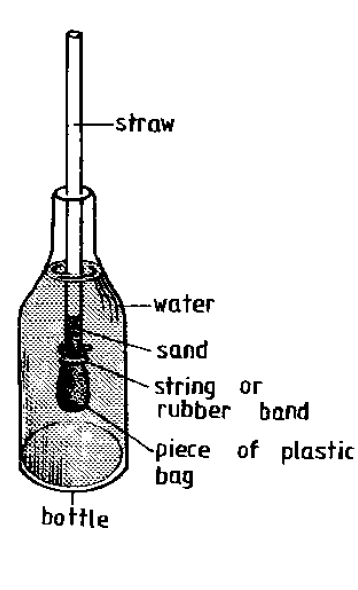
\includegraphics[width=0.35\textwidth]{./img/source/hydrometer.png}
\end{center}

\begin{description*}
%\item[Subtopic:]{}
\item[Materials:]{Bottle, straw, plastic bag, dry sand, rubber band/string, pen, ruler, water, kerosene, other liquids}
\item[Setup:]{Close one end of the straw with the plastic bag and secure it with the rubber band so that water cannot enter. Pour sand into the straw until it floats upright in the bottle of water without touching the bottom or leaning.}
\item[Procedure:]{Use a pen to mark the water level on the outside of the straw. Label it 1.0 (the density of water in g/cm$^3$). Place the straw upright in a container of kerosene. Mark the kerosene level on the straw as 0.8 (known density of kerosene). Remove and clean the straw, without getting any liquid inside. Use a ruler to complete the scale above 1.0 and below 0.8, beginning with 0.9 at the midpoint. Use the hydrometer to measure the densities of other liquids.}
%\item[Hazards:]{}
\item[Questions:]{Why do smaller numbers appear at the top of the hydrometer scale?}
%\item[Observations:]{}
\item[Theory:]{Liquids with a lower density allow the hydrometer to sink deeper, and thus the liquid reaches a higher point on the scale.}
%\item[Applications:]{}
%\item[Notes:]{}
\end{description*}


\end{multicols}

\pagebreak
\section{Structure and Properties of Matter}

\begin{multicols}{2}

\section*{States of Matter} \label{sec:states-matter} \index{Matter! states of}
%All matter is made up of particles. These particles are in constant motion which increases with their temperature. Depending on temperature, matter may exist in three states: \emph{solid}, \emph{liquid} or \emph{gas}.


\subsection{Student Particles}

\begin{center}
\includegraphics[width=0.4\textwidth]{./img/source/states-matter.png}
%\includegraphics[width=0.4\textwidth]{./img/vso/states-matter.png}
\end{center}

\begin{description*}
%\item[Subtopic:]{}
%\item[Materials:]{}
%\item[Setup:]{}
\item[Procedure:]{Use students to demonstrate the concept of states of matter.}
%\item[Hazards:]{}
%\item[Questions:]{}
%\item[Observations:]{}
\item[Theory:]{When students or objects are close together, they represent particles in the \emph{solid} state. As they move apart and past each other they represent particles in the \emph{liquid} state. Fast and randomly moving pupils or objects represent particles in the \emph{gaseous} state.}
%\item[Applications:]{}
%\item[Notes:]{}
\end{description*}

\subsection{A Model of Motion}

\begin{center}
\includegraphics[width=0.49\textwidth]{./img/vso/motion-model.jpg}
\end{center}

\begin{description*}
%\item[Subtopic:]{}
%\item[Materials:]{}
%\item[Setup:]{}
\item[Procedure:]{Put some dry beans, rice or stones in a clear bottle. Hold the bottle still, then turn it, then shake it vigorously.}
%\item[Hazards:]{}
\item[Questions:]{Which activity corresponds to which state of matter?}
%\item[Observations:]{}
\item[Theory:]{The movement of particles in solids is small and hence they are in fixed order. In liquids the particles move past each other and have lost the stiff order. In gases they move very fast and randomly, losing all order.}
%\item[Applications:]{}
%\item[Notes:]{}
\end{description*}

\subsection{Changes of State} \index{Matter! states of}

\begin{center}
\includegraphics[width=0.25\textwidth]{./img/source/change-state.png}
\end{center}

\begin{description*}
%\item[Subtopic:]{}
\item[Materials:]{Tin can, glass bottle, water, \nameref{sec:heatsources}}
%\item[Setup:]{}
\item[Procedure:]{Pour a small amount of water into a tin can and heat it until it boils. Fill a bottle with cool water and hold it above the tin can.}
%\item[Hazards:]{}
%\item[Questions:]{}
\item[Observations:]{Water drops form on the outside of the cool bottle when it is touched by the steam of the boiling water.}
\item[Theory:]{Water particles escape from the boiling water as vapour and condense on the lower surface of the bottle to form water droplets. Hence water is made up of small particles.}
%\item[Applications:]{}
%\item[Notes:]{}
\end{description*}

\subsection{Model of Brownian Movement}

\begin{center}
\includegraphics[width=0.4\textwidth]{./img/source/brownian.jpg}
\end{center}

Imagine there would be standing a tall adult person around whom small children are in a
continuous random movement. The tall person would be punched permanently by the
children and hence would be jerkily moved.

%\begin{description*}
%%\item[Subtopic:]{}
%\item[Materials:]{}
%\item[Setup:]{}
%\item[Procedure:]{}
%\item[Hazards:]{}
%\item[Questions:]{}
%\item[Observations:]{}
%\item[Theory:]{}
%\item[Applications:]{}
%\item[Notes:]{}
%\end{description*}

%\vfill
\columnbreak

%==================================================================================================%

\section*{Particulate Nature of Matter}


\subsection{Salt is Made of Particles}

\begin{center}
\includegraphics[width=0.4\textwidth]{./img/source/salt-particles.png}
\end{center}

\begin{description*}
%\item[Subtopic:]{}
\item[Materials:]{Salt/sugar, cup, water}
%\item[Setup:]{}
\item[Procedure:]{Roll some salt or sugar crystals between your fingers. Taste the crystals. Take a sip of the water. Now put the salt or sugar in the water and shake it. Taste again.}
%\item[Hazards:]{}
%\item[Questions:]{}
%\item[Observations:]{The crystals are hard and of cubical shape. They dissolve in water and the solution tastes like salt or sugar.}
\item[Theory:]{Sugar and salt are made up of tiny particles that can be identified by tasting even though they can not be seen in a solution.}
%\item[Applications:]{}
%\item[Notes:]{}
\end{description*}

\subsection{Weighing Particles}

\begin{center}
\includegraphics[width=0.49\textwidth]{./img/source/weighing-particles.png}
\end{center}

\begin{description*}
%\item[Subtopic:]{}
\item[Materials:]{\nameref{sec:balance}, small pieces of wood, \nameref{sec:heatsources}}
%\item[Setup:]{}
\item[Procedure:]{Weight pieces of wood and record the weight. Then burn the wood and weigh the ash.}
%\item[Hazards:]{}
\item[Questions:]{Is there a difference between the two weights?}
%\item[Observations:]{}
\item[Theory:]{The weight of the ash is less than that of wood. The loss in weight is due to particles which escaped as soot and gas.}
\item[Applications:]{This is why garbage reduces in size when burned. Burning wood and garbage releases carbon dioxide and other harmful gases into our environment. This is one form of \emph{pollution}.}
%\item[Notes:]{}
\end{description*}

%==================================================================================================%

\section*{Elasticity} \index{Elasticity}


\subsection{Hooke's Law} \index{Hooke's law|see{Practicals}} \index{Practicals! Hooke's law}
\textbf{*NECTA PRACTICAL*}
\begin{center}
%\includegraphics[width=0.49\textwidth]{./img/source/elasticity.png}
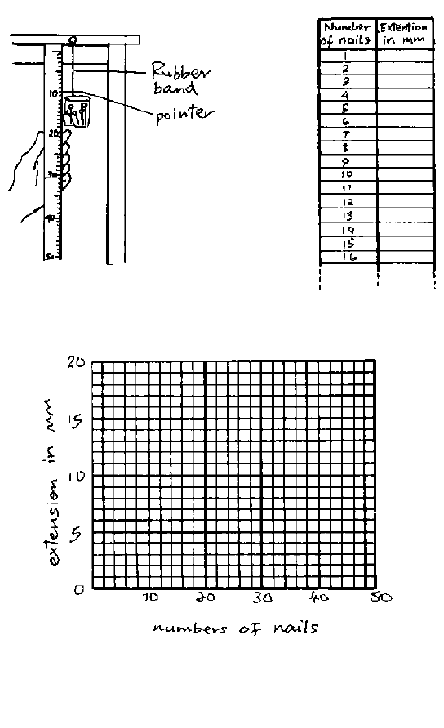
\includegraphics[width=0.49\textwidth]{./img/source/meas-mass.png}
\end{center}

\begin{description*}
%\item[Subtopic:]{}
\item[Materials:]{Rubber band/elastic strip, ruler, wire, \nameref{sec:scale-pan}, nails/small \nameref{sec:masses}, tape}
\item[Setup:]{Fix a ruler and rubber band side-by-side to a table or retort stand. At the other end of the rubber band, attach a small length of wire to act as a pointer and a small bag or scale pan (e.g. cardboard tube).}
\item[Procedure:]{Fill the scale pan with regular increments of nails or known weights. Have students measure the extension of the rubber band after each addition. Record and use the data to draw a graph of force (weight) against extension.}
%\item[Hazards:]{}
\item[Questions:]{What is the relationship between number of weights added and extension of the rubber band? What does the slope of the graph represent?}
%\item[Observations:]{}
\item[Theory:]{Hooke's Law states that the force applied to an elastic object is directly proportional to its extension ($F = kx$). The slope represents the elastic constant of the material. }
%\item[Applications:]{}
%\item[Notes:]{}
\end{description*}

%\vfill
\columnbreak

%==================================================================================================%

\section*{Adhesion and Cohesion} \index{Adhesion} \index{Cohesion}
Forces between particles of the same material are called \emph{cohesive forces} while those between particles of different materials are called \emph{adhesive forces}.


\subsection{Adhesion of Glass and Water}

\begin{center}
\includegraphics[width=0.49\textwidth]{./img/source/adhesion-cohesion.jpg}
\end{center}

\begin{description*}
%\item[Subtopic:]{}
\item[Materials:]{2 glass sheets, water, straw}
%\item[Setup:]{}
\item[Procedure:]{Drip water on a clean glass sheet (a). Place a second glass sheet on the wet first sheet and try to lift it (b).}
%\item[Hazards:]{}
%\item[Questions:]{}
%\item[Observations:]{}
\item[Theory:]{(a) Water spreads to form a patch on the first glass surface because \emph{adhesive forces}
attract water molecules to the glass surface.
(b) A strong force is required to separate the two glass sheets because the adhesive forces
between glass and water are large.}
%\item[Applications:]{}
%\item[Notes:]{}
\end{description*}

\subsection{Pinching Water}
\begin{description*}
%\item[Subtopic:]{}
\item[Materials:]{500 mL water bottle, needle/pin}
\item[Setup:]{Make 5 small holes at the bottom of the bottle with a syringe needle or nail. Make them close together (about 5 mm apart).}
\item[Procedure:]{Fill the bottle with water and allow it to flow through the holes at the bottom. Use your thumb and forefinger to pinch the streams together to form a single stream. Pass your hand over the holes and all five will appear again.}
%\item[Hazards:]{}
%\item[Questions:]{}
%\item[Observations:]{}
\item[Theory:]{Water has a tendency to cling to itself due to its surface tension and cohesion. As you bring the streams together, you allow the water to stick to itself forming a single stream. Passing your hand in front again stops the flow of water and allows it to start again in five streams.}
%\item[Applications:]{}
%\item[Notes:]{}
\end{description*}

\columnbreak

\subsection[Exploring Adhesion and Cohesion]{Exploring Adhesion and \hfill \\ Cohesion}

\begin{center}
\includegraphics[width=0.45\textwidth]{./img/adhesion-cohesion.png}
\end{center}

\begin{description*}
%\item[Subtopic:]{}
\item[Materials:]{Sheet of glass, water, honey, glycerin, cooking oil, syringe, and 2 wooden blocks}
%\item[Setup:]{}
\item[Procedure:]{Place a sheet of glass over two wooden blocks on a table. Using a syringe, place a drop of different liquids on the glass.}
%\item[Hazards:]{}
%\item[Questions:]{}
\item[Observations:]{Water spreads and wets the glass, while honey, glycerin and cooking oil remain in a spherical shape.}
\item[Theory:]{The adhesive forces between the water molecules and glass molecules are greater, while the cohesive forces between the molecules of honey, glycerin and cooking oil are larger.}
%\item[Applications:]{}
%\item[Notes:]{}
\end{description*}

\subsection{Water Drops}

\begin{center}
\includegraphics[width=0.3\textwidth]{./img/source/water-drops.png}
\end{center}

\begin{description*}
%\item[Subtopic:]{}
\item[Materials:]{Syringe or water dropper}
%\item[Setup:]{}
\item[Procedure:]{Slowly drip water from the syringe or water dropper. Observe how the drop forms.}
%\item[Hazards:]{}
%\item[Questions:]{}
\item[Observations:]{The water stream grows thinner and thinner as it moves further down and finally breaks to form drops.}
\item[Theory:]{Strong cohesive forces hold the water molecules together, until they are overcome by gravity and the water breaks off as drops.}
%\item[Applications:]{}
%\item[Notes:]{}
\end{description*}


\columnbreak

%==================================================================================================%

\section*{Surface Tension} \index{Surface tension}


\subsection{Water Dome}

\begin{center}
\includegraphics[width=0.2\textwidth]{./img/source/water-dome.png}
\end{center}

\begin{description*}
%\item[Subtopic:]{}
\item[Materials:]{Coin, water, syringe or eyedropper}
%\item[Setup:]{}
\item[Procedure:]{Place the coin flat on a table. Use the syringe or eyedropper to carefully drop individual water drops onto the coin.}
%\item[Hazards:]{}
\item[Questions:]{How many drops do you think the coin can hold?}
\item[Observations:]{The coin holds a surprising number of drops and forms a dome shape before the water spills over.}
\item[Theory:]{The surface tension of the water holds it together against the force of gravity, which is trying to pull the water off the coin.}
%\item[Applications:]{}
%\item[Notes:]{}
\end{description*}

\subsection{Pin Float}

\begin{center}
\includegraphics[width=0.49\textwidth]{./img/source/pin-float.png}
\end{center}

\begin{description*}
%\item[Subtopic:]{}
\item[Materials:]{Cup or small dish, straight pin/razor/paper clip, water, detergent}
%\item[Setup:]{}
\item[Procedure:]{Fill the cup with clean water and carefully float a pin, razor or small paper clip. Now add a small amount of detergent to the water and observe what happens.}
%\item[Hazards:]{}
%\item[Questions:]{}
\item[Observations:]{The objects float on the surface of the water initially, but after adding detergent, they sink to the bottom.}
\item[Theory:]{The surface tension of the water acts as an elastic membrane and is strong enough to support the small objects. Soap lowers the surface tension of water and therefore the objects sink.}
%\item[Applications:]{}
%\item[Notes:]{}
\end{description*}

\columnbreak

\subsection{Overflowing Glass}

\begin{center}
\includegraphics[width=0.45\textwidth]{./img/source/glass-overflow.jpg}
\end{center}

\begin{description*}
%\item[Subtopic:]{}
\item[Materials:]{Glass cup, water, nails}
%\item[Setup:]{}
\item[Procedure:]{Carefully fill a transparent glass vessel with water to the rim. Add nails, one at a time, to
the water and count the number of nails sunk just as water begins to spill over.}
%\item[Hazards:]{}
%\item[Questions:]{}
\item[Observations:]{The water surface bulges out but does not break immediately because of strong \emph{cohesion
forces} between the water particles.}
%\item[Theory:]{}
%\item[Applications:]{}
%\item[Notes:]{}
\end{description*}

\subsection{Blowing Bubbles}
\begin{description*}
%\item[Subtopic:]{}
\item[Materials:]{Thin piece of wire (approximately 30cm), water, detergent, glycerin (optional)}
\item[Setup:]{Bend the wire to form a loop of 2 to 3 cm in diameter, circling this loop many times. Leave a straight piece several cm long as a handle. Make a concentrated solution of detergent in water with a small amount of glycerin.}
\item[Procedure:]{Dip the circular part of the wire into the detergent. You should see a thin soapy film across the circle upon removal. Gently blow through the circle until a bubble separates from the wire.}
%\item[Hazards:]{}
%\item[Questions:]{}
\item[Observations:]{While blowing, the solution is being pulled back towards the surface. Once it breaks free as a bubble, it forms a spherical shape.}
\item[Theory:]{The surface tension of water causes the bubble to form the shape with the minimum surface area, which is a sphere.}
%\item[Applications:]{}
%\item[Notes:]{}
\end{description*}

\columnbreak

%==================================================================================================%

\section*{Capillarity} \index{Capillarity}


\subsection{Capillary Rise}

\begin{center}
\includegraphics[width=0.4\textwidth]{./img/source/capillary-glass.jpg}
\end{center}

\begin{description*}
%\item[Subtopic:]{}
\item[Materials:]{2 glass sheets, match, rubber bands, water, food colour (optional)}
%\item[Setup:]{}
\item[Procedure:]{With the help of a rubber band and a matchstick, arrange two clean glass sheets as shown
in the diagram. Place the arrangement in a plate containing some water.}
%\item[Hazards:]{}
%\item[Questions:]{}
\item[Observations:]{Water rises to different heights along and between the glass sheets. }
\item[Theory:]{This is capillary
action. Capillary rise results from adhesion, allowing the liquid to climb along the surface of the glass, as well as cohesion, which pulls the remainder of the liquid up. Water rises more where the glass sheets are closer together.}
%\item[Applications:]{}
%\item[Notes:]{}
\end{description*}

%\subsection{Capillary Rise}
%
%\begin{center}
%\includegraphics[width=0.4\textwidth]{./img/source/capillary-rise.jpg}
%\end{center}
%
%\begin{description*}
%%\item[Subtopic:]{}
%\item[Materials:]{Straws/chalk of different sizes, bottle, food colour, various liquids, e.g. water, spirit, kerosene, cooking oil}
%\item[Setup:]{Cut the bottom of a bottle to make a small dish.}
%\item[Procedure:]{Place one end of a straw/chalk into a dish of water 1 cm deep. Mark the change in level of the food colour after about a minute. Repeat for different liquids and different size straws.}
%%\item[Hazards:]{}
%\item[Questions:]{Which liquid rises the farthest up the straw? Do liquids rise faster in wide or thin straws?}
%\item[Observations:]{The spirit rises to the greatest height while water rises the least. Liquids rise faster in thin straws compared to thick ones.}
%\item[Theory:]{%Capillary rise results from adhesion, allowing the liquid to climb along the surface of the tube, as well as cohesion, which pulls the remainder of the liquid up. 
%In a thin container, a larger proportion of liquid is attached to the side of the tube and a smaller proportion is being held by surface tension, so the adhesive force is strong enough to pull more liquid up the tube.}
%%\item[Applications:]{}
%%\item[Notes:]{}
%\end{description*}

\subsection{Moving Matches}

%\begin{center}
%\includegraphics[width=0.4\textwidth]{./img/.png}
%\end{center}

\begin{description*}
%\item[Subtopic:]{}
\item[Materials:]{Matches, water, straw, plastic lid}
%\item[Setup:]{}
\item[Procedure:]{Break several matches near the middle, but not so that they come apart. They should make acute angles. Place them on the plastic lid and place a few drops of water on the broken joints of the matches using the straw.}
%\item[Hazards:]{}
%\item[Questions:]{}
\item[Observations:]{The matches close and return to their original straight shape.}
\item[Theory:]{Water gets absorbed in the wooden matchstick and causes it to expand.}
\item[Applications:]{This is why it is difficult to open a wooden door after it rains. The water rises up the wood causing it to expand into its frame.}
%\item[Notes:]{}
\end{description*}

\columnbreak

\subsection{Measuring Capillary Rise}

\begin{center}
\includegraphics[width=0.4\textwidth]{./img/source/capillary-rise-meas.jpg}
\end{center}

\begin{description*}
%\item[Subtopic:]{}
\item[Materials:]{Paper, chalk, small dish/lid, water, food colour}
\item[Setup:]{Cut off the bottom of a plastic bottle to make a water dish.}
\item[Procedure:]{Place a strip of paper and a piece of chalk in a dish containing water. Leave the objects for some time and measure the rise in colour of each using a ruler.}
%\item[Hazards:]{}
%\item[Questions:]{}
\item[Observations:]{The water rises faster in the chalk than in the paper.}
\item[Theory:]{Chalk has smaller capillaries than paper, which allows water to rise faster.}
%\item[Applications:]{}
%\item[Notes:]{}
\end{description*}

\subsection{Automatic Irrigation}

\begin{center}
\includegraphics[width=0.3\textwidth]{./img/source/irrigation.png}
\end{center}

\begin{description*}
%\item[Subtopic:]{}
%\item[Materials:]{}
%\item[Setup:]{}
%\item[Procedure:]{}
%\item[Hazards:]{}
%\item[Questions:]{}
%\item[Observations:]{}
%\item[Theory:]{}
\item[Applications:]{Capillary action can be used to provide automatic irrigation for plants. Students can perform irrigation by dipping a porous material such as paper or cotton cloth in water.}
%\item[Notes:]{}
\end{description*}

\columnbreak

%==================================================================================================%

\section*{Diffusion} \index{Diffusion}

\subsection{Diffusion in Liquids}

\begin{center}
\includegraphics[width=0.4\textwidth]{./img/vso/diffusion.jpg}
\end{center}

\begin{description*}
%\item[Subtopic:]{}
\item[Materials:]{Plastic water bottle, food colour (liquid or powder)}
%\item[Setup:]{}
\item[Procedure:]{Put a drop or small amount of powdered food colour into the water without shaking and observe what happens.}
%\item[Hazards:]{}
%\item[Questions:]{}
\item[Observations:]{The colour gradually spreads throughout the water.}
\item[Theory:]{This spreading is due to the motion of the particles of food colour. This process is called \emph{diffusion}.}
\item[Applications:]{Organisms utilize diffusion to balance nutrient concentrations in cells and to transfer oxygen into the bloodstream during respiration.}
%\item[Notes:]{}
\end{description*}

\subsection{Smelling Particles}

\begin{center}
\includegraphics[width=0.4\textwidth]{./img/source/smelling-particles.jpg}
\end{center}

\begin{description*}
%\item[Subtopic:]{}
\item[Materials:]{Orange or other citrus fruit, box}
%\item[Setup:]{}
\item[Procedure:]{Peel and orange and have students raise their hands when they begin to smell it. Now place a box in front of the orange and repeat the test.}
%\item[Hazards:]{}
%\item[Questions:]{}
\item[Observations:]{Students in the front center of the room should be the first to raise their hands, followed by those near the sides and in the back. When the orange is peeled behind the box it takes longer for the smell to reach the students.}
\item[Theory:]{Tiny particles from the orange peel spread by diffusion to students' noses. The box hinders the motion of the particles and so they reach the students more slowly.}
\item[Applications:]{Air fresheners and other sprays}
%\item[Notes:]{}
\end{description*}

\subsection{Diffusion in Daily Life}

\begin{center}
\includegraphics[width=0.49\textwidth]{./img/source/diffusion-life.jpg}
\end{center}

\begin{description*}
%\item[Subtopic:]{}
%\item[Materials:]{}
%\item[Setup:]{}
\item[Procedure:]{Pass near a place where people are roasting meat or cooking.}
%\item[Hazards:]{}
%\item[Questions:]{}
%\item[Observations:]{}
\item[Theory:]{The smell is sensed even at a distance, because the particles which produce the smell
spread by \emph{diffusion}.}
%\item[Applications:]{}
%\item[Notes:]{}
\end{description*}

\subsection{Diffusion and Pollution} \index{Pollution}

\begin{center}
\includegraphics[width=0.49\textwidth]{./img/source/diffusion-pollution.jpg}
\end{center}

\begin{description*}
%\item[Subtopic:]{}
%\item[Materials:]{}
%\item[Setup:]{}
\item[Procedure:]{Pass near a polluted area (e.g. latrine, burning heaps of litter, a filling station).}
%\item[Hazards:]{}
%\item[Questions:]{}
%\item[Observations:]{}
\item[Theory:]{Many hazardous substances spread to the environment by diffusion. (Hazardous
substances in any state of matter in our environment mean pollution.)}
%\item[Applications:]{}
%\item[Notes:]{}
\end{description*}

\columnbreak

%==================================================================================================%

\section*{Osmosis} \index{Osmosis}


\subsection{Vanilla Balloon}

\begin{center}
\includegraphics[width=0.35\textwidth]{./img/vso/osmosis-vanilla.jpg}
\end{center}

\begin{description*}
%\item[Subtopic:]{}
\item[Materials:]{Balloon/plastic bag, vanilla, straw/syringe}
%\item[Setup:]{}
\item[Procedure:]{Place a few drops of vanilla in a deflated balloon. Now blow up the balloon and tie it shut.}
%\item[Hazards:]{}
%\item[Questions:]{}
\item[Observations:]{You can smell the vanilla through the surface of the balloon.}
\item[Theory:]{The balloon acts as a \emph{semi-permeable membrane} which allows some of the vanilla particles to pass through and reach your nose. Other particles remain inside the balloon.}
%\item[Applications:]{}
%\item[Notes:]{}
\end{description*}

\subsection{Potato Osmosis}

\begin{center}
\includegraphics[width=0.49\textwidth]{./img/vso/osmosis-potato-full.jpg}
\end{center}

\begin{description*}
%\item[Subtopic:]{}
\item[Materials:]{Potato, 2 water bottles, salt, water}
\item[Setup:]{Cut two equal size pieces of potato. Fill one bottle with fresh water and the other with a salt water solution.}
\item[Procedure:]{Put one piece of potato in each bottle. Observe over the next few hours.}
%\item[Hazards:]{}
%\item[Questions:]{}
\item[Observations:]{The potato in fresh water swells while the potato in salt water shrivels up.}
\item[Theory:]{Through osmosis, water moves from a region of low concentration to one of high concentration through a semi-permeable membrane (the potato). In fresh water, the potato has the higher salt concentration, so water enters in order to make a balance. In salt water, the concentration of the surrounding water is higher than that of the potato, so water inside the potato moves outside to dilute the salt solution.}
%\item[Applications:]{}
\item[Notes:]{Try this experiment again with a boiled potato. Do you observe any differences?}
\end{description*}

\columnbreak

\subsection{Semi-Permeable Membranes}

\begin{center}
\includegraphics[width=0.4\textwidth]{./img/vso/membrane.jpg}
\end{center}

\begin{description*}
%\item[Subtopic:]{}
\item[Materials:]{Glass jar, clear plastic bag, small beads or stones, beans, netting, string/rubber band}
\item[Setup:]{Place the mixture of beads and beans in the jar. Place the net and plastic bag over the top and tie them on securely.}
\item[Procedure:]{Shake the apparatus for a few seconds.}
%\item[Hazards:]{}
%\item[Questions:]{}
\item[Observations:]{Only the small beads pass through the netting. The beans remain in the jar.}
\item[Theory:]{The beads represent small molecules and the net is a semi-permeable membrane. The beans are too large to pass through and hence remain in the jar.}
\item[Applications:]{Water filters, organism cell membranes}
%\item[Notes:]{}
\end{description*}

\subsection{Osmosis with Eggs} % VSO 25

\begin{center}
\includegraphics[width=0.4\textwidth]{./img/vso/osmosis-eggs.jpg}
\end{center}

\begin{description*}
%\item[Subtopic:]{}
\item[Materials:]{Empty eggshell, strong salt solution, jar of water}
%\item[Setup:]{}
\item[Procedure:]{Remove the hard outer shell at
one end of the eggshell to
expose the inner membrane. Half
fill the egg with salt solution and
place it in the jar so that the
water level is above the exposed
membrane and leave for a couple
of hours. }
%\item[Hazards:]{}
\item[Observations:]{The level of
the solution inside the egg rises,
indicating water has crossed the
membrane, i.e. osmosis has
occurred.}
%\item[Questions:]{What happens if you use sugar solution instead of salt? What if you put salt solution in the jar as well as the egg?}
\item[Theory:]{Water travels from an area of low concentration to an area of high concentration of salts.}
%\item[Applications:]{}
%\item[Notes:]{}
\end{description*}


\end{multicols}

\pagebreak
\section{Pressure}
\label{sec:pressure}

\begin{multicols}{2}


\section*{Concept of Pressure}
%\textbf{Pressure} is the force acting normally per unit surface area. \\
%$\text{Pressure} = \text{Force} \div \text{Area} $


\subsection{What is Pressure?}

\begin{center}
\includegraphics[width=0.49\textwidth]{./img/source/pressure.jpg}
\end{center}

\begin{description*}
%\item[Subtopic:]{}
\item[Materials:]{Pencil, book}
%\item[Setup:]{}
\item[Procedure:]{Ask a student to support a book as shown in figure (a). Then turn the pencil upside down
as shown in figure (b).}
%\item[Hazards:]{}
%\item[Questions:]{}
\item[Observations:]{In case (b) the student will feel pain on the hand supporting the pencil.}
\item[Theory:]{In case (b) the force with which the pencil acts on the hand is the same (equal to the
weight of book plus pencil) as in case (a) but the pressure on the hand has increased very
much since the area on which the pencil touches the hand has decreased so much.}
\item[Applications:]{Large area feet of elephants; wide tyres of tractors; wide chains of caterpillar machines.}
%\item[Notes:]{}
\end{description*}


\subsection{Balloon Pop}

%\begin{center}
%\includegraphics[width=0.4\textwidth]{./img/.png}
%\end{center}

\begin{description*}
%\item[Subtopic:]{}
\item[Materials:]{2 pieces of wood, nails, balloons, water}
\item[Setup:]{Put a single nail through one piece of wood and for the other, put many nails closely spaced. Blow up 2 balloons or fill them with water.}
\item[Procedure:]{Slowly press one balloon against the single nail until it pops. Then repeat for the cluster of nails.}
%\item[Hazards:]{}
%\item[Questions:]{}
\item[Observations:]{The balloon pops easily on the single nail, though it may not pop at all on the cluster of nails.}
\item[Theory:]{Using many nails increases the area over which the force of the nails act, thus decreasing the pressure and requiring a greater force to make the balloon pop.}
%\item[Applications:]{}
\item[Notes:]{You can also hang the balloon from a spring balance as you lower it onto the nails. The difference in weight gives the force needed to pop the balloon.}
\end{description*}

\columnbreak

\subsection{Carrying a Load on the Head}

\begin{center}
\includegraphics[width=0.4\textwidth]{./img/source/load-head.png}
\end{center}

\begin{description*}
%\item[Subtopic:]{}
%\item[Materials:]{}
%\item[Setup:]{}
\item[Procedure:]{Carry a bucket on your head without (a) and with (b) a cloth or khanga.}
%\item[Hazards:]{}
\item[Questions:]{Which is more difficult?}
%\item[Observations:]{}
\item[Theory:]{Using the cloth causes the force of the bucket to be more evenly distributed across a larger area. Hence the force felt at any single point is reduced.}
%\item[Applications:]{}
%\item[Notes:]{}
\end{description*}

\subsection{Potato Poke}

%\begin{center}
%\includegraphics[width=0.4\textwidth]{./img/.png}
%\end{center}

\begin{description*}
%\item[Subtopic:]{}
\item[Materials:]{Straw, potato}
%\item[Setup:]{}
\item[Procedure:]{Try to stab a straw into the potato. Now place your thumb firmly over one end of the straw and try again.}
%\item[Hazards:]{}
%\item[Questions:]{}
\item[Observations:]{The straw bends easily and does not harm the potato the first time. When you cover one end of the straw, it enters the potato easily and may even break through the other side.}
\item[Theory:]{Holding your thumb over the straw traps air inside which increases the pressure in the straw. When it strikes the potato, the increased pressure prevents it from bending and so it is able to poke through the potato.}
%\item[Applications:]{}
%\item[Notes:]{}
\end{description*}

\columnbreak

%==================================================================================================%

\section*{Pressure in Solids}


\subsection[Effect of Surface Area on Pressure]{Effect of Surface Area on \hfill \\ Pressure}

\begin{center}
%\includegraphics[width=0.4\textwidth]{./img/pressure-solid1.png}
%\includegraphics[width=0.4\textwidth]{./img/pressure-solid2.png}
\includegraphics[width=0.4\textwidth]{./img/pressure-solids.png}
\end{center}

\begin{description*}
%\item[Subtopic:]{}
\item[Materials:]{Bar of soap, thin thread, thick string, 4 heavy stones of approximately equal weight}
%\item[Setup:]{}
\item[Procedure:]{Tie a heavy stone to either end of both the thin thread and thick string. Hang each thread across the bar of soap so that the weights hang freely.}
%\item[Hazards:]{}
%\item[Questions:]{}
\item[Observations:]{The thin thread easily cuts through the soap, but the thick string does not.}
\item[Theory:]{The smaller area of the thin thread, acting with the same force, results in an increased pressure which is enough to cut through the soap.}
%\item[Applications:]{}
%\item[Notes:]{}
\end{description*}

\vfill
\columnbreak

%==================================================================================================%

\section*{Pressure in Liquids}


\subsection{Pressure Increases with Depth}

\begin{center}
\includegraphics[width=0.3\textwidth]{./img/source/pressure-depth.png}
\end{center}

\begin{description*}
%\item[Subtopic:]{}
\item[Materials:]{1.5 L bottle, syringe needle or pin/nail, water}
\item[Setup:]{Poke three holes into a bottle. Put one hole near the bottom, one near the middle, and the last hole between them.}
\item[Procedure:]{Fill the bottle with water and place on a table. Observe the trajectories of water coming from the three holes.}
%\item[Hazards:]{}
\item[Questions:]{Which stream goes the farthest distance horizontally? Which hole has the highest pressure?}
\item[Observations:]{The water flowing from the lower holes travels farther.}
\item[Theory:]{The added weight of the water above the lower holes increases the pressure there, resulting in an increased horizontal velocity. It is shown that pressure increases with depth ($P = \rho g h$).}
\item[Applications:]{The wall of a dam is made much thicker at the bottom than at the top. This is to reinforce against the increased water pressure at greater depths.}
%\item[Notes:]{}
\end{description*}

\subsection{Pressure Acts in All Directions}

\begin{center}
\includegraphics[width=0.4\textwidth]{./img/source/pressure-direction.png}
\end{center}

\begin{description*}
%\item[Subtopic:]{}
\item[Materials:]{Water bottle/balloon/plastic bag, pin/needle, water}
%\item[Setup:]{}
\item[Procedure:]{Fill a bottle, balloon or plastic bag with water. Poke several small holes around the surface.}
%\item[Hazards:]{}
%\item[Questions:]{}
\item[Observations:]{Water is expelled equally through all of the holes.}
\item[Theory:]{Pressure in a liquid acts equally in all directions.}
%\item[Applications:]{}
%\item[Notes:]{}
\end{description*}

\subsection{Straw Fountain}

\begin{center}
\includegraphics[width=0.25\textwidth]{./img/vso/straw-fountain.jpg}
\end{center}

\begin{description*}
%\item[Subtopic:]{}
\item[Materials:]{500 mL water bottle with cap, water, straw, glue, hot nail/pin}
\item[Setup:]{Poke a hole the size of the straw in the bottle cap using a heated nail or pin. Stick the straw through the hole and screw on the cap so that the straw reaches near the bottom. Glue around the straw so that it is air tight.}
\item[Procedure:]{Fill the bottle about half way with water and close the cap with the straw inside. Have a student blow as hard as they can through the straw into the water and then stop.}
%\item[Hazards:]{}
%\item[Questions:]{}
\item[Observations:]{When the student stops blowing, they get sprayed in the face by water.}
\item[Theory:]{Blowing into the bottle greatly increases the pressure inside. When you stop blowing, the pressure equalizes by forcing water back out through the straw.}
%\item[Applications:]{}
%\item[Notes:]{}
\end{description*}

\subsection{Hydraulic Press}

\begin{center}
\includegraphics[width=0.3\textwidth]{./img/source/hydraulic-press.png}
\end{center}

\columnbreak

\begin{description*}
%\item[Subtopic:]{}
\item[Materials:]{2 syringes of different size (5 mL and 20 mL), \nameref{sec:delivery-tube}, water}
\item[Setup:]{Fill the larger syringe with water and attach one end of the rubber tubing to its end. Attach the other end of the tubing to the smaller syringe (with its plunger inserted all the way).}
\item[Procedure:]{Pushing the plunger of the larger syringe will cause the plunger of the smaller syringe to go out, and vice-versa.}
%\item[Hazards:]{}
%\item[Questions:]{}
\item[Observations:]{It is easier to push the plunger of the small syringe than that of the larger syringe.}
\item[Theory:]{Pascal's principle states that pressure is distributed equally throughout a liquid. Thus, the pressure at one plunger must be equal to the pressure at the other plunger. Setting the two ratios equal, we can see that a small force over a small area can overcome a large force over a large area.}
\item[Applications:]{Industrial machinery, hydraulic breaks}
%\item[Notes:]{}
\end{description*}

\subsection{The Manometer}

\begin{center}
\includegraphics[width=0.48\textwidth]{./img/source/manometer.png}
\end{center}

\begin{description*}
%\item[Subtopic:]{}
\item[Materials:]{\nameref{sec:delivery-tube}, ruler, cardboard, string, water, food colour, water bottle}
\item[Setup:]{Create the manometer as shown by attaching thin tubing in a U-shape to a cardboard stand and filling with a small amount of coloured water. Make sure there is sufficient length of tubing left over on either side.}
\item[Procedure:]{Insert each arm of the manometer to a different depth in a bottle of water.}
%\item[Hazards:]{}
%\item[Questions:]{}
\item[Observations:]{When both arms are at equal pressure, the water levels are equal. When one side experiences a higher pressure, there is a noticeable difference in the height $h$ of coloured water on the opposite side.}
\item[Theory:]{A manometer is used to measure fluid pressure. When the pressure is higher on one side, it is shown by a difference in height on the manometer which can be measured. The greater the pressure difference, the higher the value of $h$.}
%\item[Applications:]{}
%\item[Notes:]{}
\end{description*}

%==================================================================================================%

\section*{Atmospheric Pressure}
\label{sec:atm-pressure}


\subsection{Overturned Glass}

\begin{center}
\includegraphics[width=0.4\textwidth]{./img/source/overturned-glass.png}
\end{center}

\begin{description*}
%\item[Subtopic:]{}
\item[Materials:]{Cup/glass, card, water}
%\item[Setup:]{}
\item[Procedure:]{Fill a cup to the rim with water. Push a smooth card from the side to cover the glass so that no air bubbles are included. Turn the glass upside down.}
%\item[Hazards:]{}
\item[Questions:]{Why can there be no air bubbles inside the glass?}
\item[Observations:]{The card remains attached to the glass and the water does not fall out.}
\item[Theory:]{The card is held in place by atmospheric pressure pushing upwards, which is larger than the weight of the water pushing downwards, so the card does not fall.}
%\item[Applications:]{}
%\item[Notes:]{}
\end{description*}

\subsection{Holey Bottle}

%\begin{center}
%\includegraphics[width=0.4\textwidth]{./img/.png}
%\end{center}

\begin{description*}
%\item[Subtopic:]{}
\item[Materials:]{Water bottle, pin, water}
%\item[Setup:]{}
\item[Procedure:]{Poke 4 or 5 small holes in the bottom of the bottle. Fill it half way with water, allowing it to spill out the holes in the bottom. Then cap the bottle and observe what happens.}
%\item[Hazards:]{}
%\item[Questions:]{}
\item[Observations:]{When the bottle is capped, the water stops flowing through the holes.}
\item[Theory:]{When the bottle is open, gravity is strong enough to pull the water through the bottom holes. When closed, however, the low pressure inside the bottle and the high atmospheric pressure outside creates an upward force that is able to overcome gravity and prevent water from flowing.}
%\item[Applications:]{}
%\item[Notes:]{}
\end{description*}

\subsection{Bottle Crush}

\begin{center}
\includegraphics[width=0.45\textwidth]{./img/source/bottle-crush.png}
\end{center}

\begin{description*}
%\item[Subtopic:]{}
\item[Materials:]{Plastic water bottle, boiling water, cold water}
%\item[Setup:]{}
\item[Procedure:]{Pour some boiling water into the bottle and cap it immediately. Shake it to make sure all the air inside is heated. Then pour cold water on the bottle.}
%\item[Hazards:]{}
%\item[Questions:]{}
\item[Observations:]{Upon pouring the cold water, the bottle crushes.}
\item[Theory:]{When the hot air inside the water bottle is cooled off, its volume decreases, leaving a partial vacuum inside the bottle. The greater atmospheric pressure outside crushes the bottle inwards.}
%\item[Applications:]{}
%\item[Notes:]{This is an application of Charles' Law. For more, see \nameref{}.}
\end{description*}

\subsection{Automatic Flushing Tank}
\label{sub:auto-tank}

\begin{center}
\includegraphics[width=0.25\textwidth]{./img/auto-flushing-tank.png}
\end{center}

\begin{description*}
%\item[Subtopic:]{}
\item[Materials:]{Empty water bottle, straw, water, bucket, super glue}
\item[Setup:]{Cut the top off of a water bottle and make a hole at the bottom for a straw to fit through. Bend the straw inside the bottle as shown and seal with super glue.}
\item[Procedure:]{Fill the bottle up to and above the bend in the straw and observe what happens.}
%\item[Hazards:]{}
%\item[Questions:]{}
\item[Observations:]{The water will flow into the bucket through the bent straw.}
\item[Theory:]{The combined pressure of the water and the atmosphere pushing down on the water is greater then the air pushing up on the straw. The tank does not require a handle to trigger the flush. Once the water flows into the tank up to the level of the siphon, the tank will flush automatically. }
%\item[Applications:]{}
%\item[Notes:]{}
\end{description*}

\columnbreak

\subsection{The Barometer}

\begin{center}
\includegraphics[width=0.3\textwidth]{./img/source/barometer.png}
\end{center}

\begin{description*}
%\item[Subtopic:]{}
\item[Materials:]{Bottle, plastic bag, string/rubber band, straw, glue, cardboard, pen}
%\item[Setup:]{}
\item[Procedure:]{Close a bottle air-tight using a piece of plastic bag and string/rubber band. Glue the straw onto the middle of the plastic and point it to a vertical scale written on paper or cardboard.}
%\item[Hazards:]{}
%\item[Questions:]{}
%\item[Observations:]{}
\item[Theory:]{When the air pressure increases, it pushes downward on the plastic and the straw dips down. When the air pressure decreases, the relatively high pressure inside the bottle pushes the plastic up, raising the straw.}
%\item[Applications:]{}
%\item[Notes:]{}
\end{description*}

\subsection{Madgeburg Hemisphere}

%\begin{center}
%\includegraphics[width=0.4\textwidth]{./img/.png}
%\end{center}

\begin{description*}
%\item[Subtopic:]{}
\item[Materials:]{2 equal size cooking pots, oil, matches, small pieces of paper}
\item[Setup:]{Spread oil or grease around the edge of one of the cooking pots.}
\item[Procedure:]{Place small papers in the un-greased pot and light them on fire. Allow them to burn about half way and then cover with the greased pot so that no air can escape. Allow the pots to cool and try to separate them.}
%\item[Hazards:]{}
%\item[Questions:]{}
\item[Observations:]{After the pots have cooled it is very difficult to separate them.}
\item[Theory:]{When you burn the paper, the air in the pot expands and escapes. When you cover the pots, no more air can enter and the air inside cools, reducing the pressure inside the pots while the pressure outside the pots remains the same. The atmospheric pressure therefore presses the pots together so as to equalize the pressure on either side. }
%\item[Applications:]{}
%\item[Notes:]{}
\end{description*}

\columnbreak

%==================================================================================================%

\section*{Applications of Atmospheric Pressure}


\subsection{The Siphon}

\begin{center}
\includegraphics[width=0.4\textwidth]{./img/source/siphon.png}
\end{center}

\begin{description*}
%\item[Subtopic:]{}
\item[Materials:]{2 containers/bottles, \nameref{sec:delivery-tube}, (1 m), water}
%\item[Setup:]{}
\item[Procedure:]{Place one bottle full of water on a table and the other below. Place one end of the tubing into the water and suck on the other end until water starts coming out. Place this end of the tube into the empty bottle and observe what happens.}
\item[Hazards:]{Clean off the tube thoroughly between uses.}
%\item[Questions:]{}
\item[Observations:]{The water continues to flow to the empty bottle despite an initial uphill climb.}
\item[Theory:]{Sucking on the tube creates a low pressure on that end. The higher atmospheric pressure on the water end causes the water to flow from high pressure to low pressure, overcoming gravity.}
\item[Applications:]{Toilets, drainage systems, \nameref{sub:auto-tank}}
\item[Notes:]{Alternatively, submerge the entire tube initially, then pinch on end and remove from the water. Upon releasing the pinched end outside of the water, the water will flow.}
\end{description*}

%\subsection{Reverse Air Pump} %?%
%
%\begin{center}
%\includegraphics[width=0.4\textwidth]{./img/.png}
%\end{center}
%
%\begin{description*}
%%\item[Subtopic:]{}
%\item[Materials:]{}
%\item[Setup:]{}
%\item[Procedure:]{}
%\item[Hazards:]{}
%\item[Questions:]{}
%\item[Observations:]{}
%\item[Theory:]{}
%\item[Applications:]{}
%\item[Notes:]{}
%\end{description*}

%\subsection{Reverse Air Pump}
%\begin{itemize}
%\item{Preparation Time: varies, about 1 hour}
%\item{Materials: Bicycle pump (the tall, metal kind), short piece of rubber tubing fitted to pump valves, utility knife, tightening sleeves, extra valve}
%\item{Procedure: There are two parts of the pump that control the direction of airflow: the first is a diaphragm inside the pump and the second is a ball valve at the base of the pump in the hose.
%\begin{enumerate}
%\item{You need to open the pump and pull out the ‘dipstick’ with the diaphragm attached. At the bottom, there should be a diaphragm with holes around the top, a metal disc the same diameter as the diaphragm, and a few nuts and washers to keep it all together. In its normal configuration, the diaphragm is pulled down by friction away from the disc when the pump handle is pulled up, allowing air to enter the pump freely. When the pump handle is pushed in, the diaphragm is forced against the disc, restricting any back airflow, and forcing all the air forward through the hose. Switch the position and direction of the diaphragm and disc so that it has the opposite effect when the pump handle is pulled in or out.}
%\item{Next, you need to cut open the hose at the base of the pump and find the valve with the small bead inside. Normally, when air is forced forward through the valve, the bead does not restrict any airflow. When air tries to go back through the pump, the bead blocks the valve and stops any airflow. Switch the direction of the valve.}
%\item{From here, you need to reattach the hose to the pump. You may need to get another nozzle to attach to the pump, attaching the hose with reversed valve with the extra bit of rubber tubing. It depends on your pump, but if you have made it this far, you will find a way to make it work. Tightening sleeves will come in handy here to make sure no air is lost after all this cutting and jury-rigging.}
%\end{enumerate}
%} % Procedure
%\item{Applications: This suction pump is great for showing the gas laws and boiling points: suck the air out of a jar of water and watch the water boil, you could also kill stuff in the jar this way, but that is just morbid, and possibly cool, or that sound travels through a medium.}
%\end{itemize}


\end{multicols}

\pagebreak
\section{Work, Energy and Power} 
%\begin{center}
%$\text{\textbf{Work}} = \text{Force} \times \text{distance in direction of Force} $\\
%Unit = 1 N $\times$ m = 1 J (Joule)\\
%\textbf{Energy} is the ability to do work. Unit = 1 J (Joule)\\
%$\text{\textbf{Power}} = \text{Work Done} \div \text{time} $\\
%Unit = 1 J $\div$ 1 s = 1 W (Watt)
%\end{center}

\begin{multicols}{2}


\section*{Work} \index{Work}


\subsection{Work Done by Lifting}

\begin{center}
\includegraphics[width=0.25\textwidth]{./img/source/work-lifting.png}
\end{center}

\begin{description*}
%\item[Subtopic:]{}
\item[Materials:]{\nameref{sec:spring-balance}, block of wood, ruler}
%\item[Setup:]{}
\item[Procedure:]{Raise a block of wood from a table using a spring balance. Read the balance while lifting at \emph{constant velocity}, not when starting or stopping. Compare this to the weight of the block. Measure the vertical distance raised $h$. }
%\item[Hazards:]{}
%\item[Questions:]{Calculate the work done when the block is raised a vertical distance $h$.}
%\item[Observations:]{}
\item[Theory:]{$\text{Work done} = \text{Weight} \times h$}
%\item[Applications:]{}
%\item[Notes:]{}
\end{description*}

\subsection{Work Done by Friction}

\begin{center}
\includegraphics[width=0.4\textwidth]{./img/source/work-friction.png}
\end{center}

\begin{description*}
%\item[Subtopic:]{}
\item[Materials:]{\nameref{sec:spring-balance}, block of wood, ruler}
%\item[Setup:]{}
\item[Procedure:]{Place the block of wood on a table and pull with constant velocity using a spring balance. Measure the distance moved by the block.}
%\item[Hazards:]{}
%\item[Questions:]{Calculate the work done from the spring balance and measured distance $x$.}
%\item[Observations:]{}
\item[Theory:]{Because the block is moving at constant velocity (no net force), the force which pulls the block is equal to the force of friction and opposite in magnitude. Thus, $\text{Work done} = \text{Force of friction} \times x$}
%\item[Applications:]{}
%\item[Notes:]{}
\end{description*}

%==================================================================================================%

\section*{Energy} \index{Energy}


\subsection{Forms of Energy}

\begin{center}
\includegraphics[width=0.5\textwidth]{./img/vso/forms-energy.jpg}
\end{center}

\begin{description*}
%\item[Subtopic:]{}
%\item[Materials:]{}
%\item[Setup:]{}
%\item[Procedure:]{}
%\item[Hazards:]{}
%\item[Questions:]{}
%\item[Observations:]{}
\item[Theory:]{Energy can take many forms, including potential, kinetic, chemical, heat, sound and electrical. \emph{Potential energy} is energy which is stored is some medium, e.g. spring or battery. \emph{Kinetic energy} is energy in motion, e.g. football or running person.}
\item[Applications:]{What other examples of energy can be found in our daily lives?}
%\item[Notes:]{}
\end{description*}

\subsection{A Slingshot}

\begin{center}
\includegraphics[width=0.4\textwidth]{./img/source/slingshot.png}
\end{center}

\begin{description*}
%\item[Subtopic:]{}
\item[Materials:]{Rubber band, branched stick, stone}
%\item[Setup:]{}
\item[Procedure:]{Tie either end of a rubber band to the branches of the stick. Place a stone in the middle of the band, pull back and release.}
\item[Hazards:]{Aim the slingshot away from all people.}
%\item[Questions:]{}
%\item[Observations:]{}
\item[Theory:]{The rubber band stores potential energy when stretched, which is transferred to the stone as kinetic energy upon release.}
%\item[Applications:]{}
\item[Notes:]{Conduct an experiment to determine the relationship between stretched length of the rubber band and distance traveled by the stone.}
\end{description*}

\subsection[Potential Energy of a Clothespin]{Potential Energy of a \hfill \\ Clothespin}

\begin{center}
\includegraphics[width=0.45\textwidth]{./img/source/energy-clothespin.png}
\end{center}

\begin{description*}
%\item[Subtopic:]{}
\item[Materials:]{Three clothespins, scissors}
%\item[Setup:]{}
\item[Procedure:]{Tie the handles of a spring clothespin together with one loop of string. Place it in between two other clothespins on a flat table as shown. Cut or burn the string.}
%\item[Hazards:]{}
%\item[Questions:]{}
\item[Observations:]{The two clothespins on either side fly off in opposite directions.}
\item[Theory:]{The spring in the clothespin stores potential energy which is released when the string is cut. This energy is converted into kinetic energy, seen by the movement of the other clothespins.}
%\item[Applications:]{}
%\item[Notes:]{}
\end{description*}

\subsection{The Steam Engine}

\begin{center}
\includegraphics[width=0.49\textwidth]{./img/vso/steam-engine.jpg}
\end{center}

\begin{description*}
%\item[Subtopic:]{}
\item[Materials:]{Tin can with lid, pin, cork, \nameref{sec:heatsources}, 2 straws}
\item[Setup:]{Poke a small hole near the top of the tin can. Make sure the lid fits tightly, but has a safety bung (i.e. cork). Mount a straw on a pin so that it may spin freely.}
\item[Procedure:]{Fill the can half way with water and heat until boiling. Hold the straw spinner near the hole in the tin.}
\item[Hazards:]{Make sure the safety bung is not too tight and that the tin is not filled with water.}
%\item[Questions:]{}
%\item[Observations:]{}
\item[Theory:]{The candle or burner transfers heat energy to the tin and hence water. This heat energy in the water molecules is converted to kinetic energy as they are forced out of the tin hole. This mechanical energy is transferred to the spinner and makes it turn.}
\item[Applications:]{Mount the steam engine to a small raft and place in water to make a steam boat.}
%\item[Notes:]{}
\end{description*}

\columnbreak

\subsection{The Simple Pendulum} \index{Pendulum! simple}

\begin{center}
\includegraphics[width=0.2\textwidth]{./img/source/pendulum.png}
\end{center}

\begin{description*}
%\item[Subtopic:]{}
\item[Materials:]{Stone, string}
%\item[Setup:]{}
\item[Procedure:]{Suspend a stone on a long string and hang from a table. Displace the pendulum to one side and release.}
%\item[Hazards:]{}
%\item[Questions:]{}
\item[Observations:]{The pendulum swings back and forth at near regular intervals.}
\item[Theory:]{When the pendulum is released from one side, it has a maximum height and hence potential energy (P.E.), but no kinetic energy (K.E.). When it reaches the low point of its swing, it has maximum velocity and hence K.E., but its P.E. is a minimum. Thus the pendulum's energy is constantly being converted between P.E. and K.E.}
%\item[Applications:]{}
%\item[Notes:]{}
\end{description*}

%==================================================================================================%

\section*{Power} \index{Power}


\subsection{Stair Power}

\begin{center}
\includegraphics[width=0.38\textwidth]{./img/source/power-2.jpg}
\end{center}

\begin{description*}
%\item[Subtopic:]{}
%\item[Materials:]{}
%\item[Setup:]{}
\item[Procedure:]{Measure the vertical height above ground of the first floor of a building. Run up to
that floor as fast as you can while your friend times you with a watch. Take your weight.}
%\item[Hazards:]{}
%\item[Questions:]{}
%\item[Observations:]{}
\item[Theory:]{Using your weight and the height of the first floor above ground, first calculate the potential
energy (PE) of your body when it is on the first floor (PE = weight $\times$ height). This is the energy given out in order to raise your body to that height.
Now calculate your power by dividing that energy by the time (in seconds) you needed to
run up.}
%\item[Applications:]{}
%\item[Notes:]{}
\end{description*}

%==================================================================================================%

%\subsection{Mousetrap Car}
%
%\begin{center}
%\includegraphics[width=0.4\textwidth]{./img/source/.png}
%\end{center}
%
%\begin{description*}
%\item[Subtopic:]{}
%\item[Materials:]{}
%\item[Setup:]{}
%\item[Procedure:]{}
%\item[Hazards:]{}
%\item[Questions:]{}
%\item[Observations:]{}
%\item[Theory:]{}
%\item[Applications:]{}
%\item[Notes:]{}
%\end{description*}

%==================================================================================================%

%\section*{Power}


%==================================================================================================%
%==================================================================================================%

% NOT USED

%\subsection{Work as Heat, Part A}
%\begin{itemize}
%\item{Preparation time: 5 minutes}
%\item{Materials: thin strip of metal, pliers}
%\item{Procedure: Take a piece of metal. Use a set of pliers to bend the metal back and forth. Feel the temperature of the metal.}
%\item{Theory: Work can manifest itself in a variety of ways. One of the most common ways is the rise in temperature. By moving the metal back and forth, you are doing work on the metal. This work is converted into heat. This heat is evidenced by the rise in temperature in the metal. }
%\end{itemize}
%
%\subsection{Work as Heat, Part B}
%\begin{itemize}
%\item{Preparation time: 0 minutes}
%\item{Materials: radio antennas, old or new }
%\item{Procedure: The radio antennas operate in a telescopic motion. Pull the radio antenna in and out for one full minute. Do not break the antenna in this movement. Observe the temperature of the antenna after the work is over.}
%\item{Theory: Again, you are doing work on the radio antenna by moving it in an out quickly. Through this action, the antenna heats up. This is the evidence of the work you have been doing. Work is defined as force times distance or. In this case, the force is the effort required to move the antenna in and out while the distance is the length of the antenna.}
%\end{itemize}
%
%\subsection{Work as Light}
%\begin{itemize}
%\item{Preparation time: 0 minutes}
%\item{Materials: duct tape, or other tape that holds together tightly.}
%\item{Procedure: Cut two pieces of duct tape. Press the ends of the bottom pieces of tape together but allow the top pieces of tape to be apart. Hold tightly to both pieces of tape at the top, and quickly rip them apart. Observe the blue light when the tape comes apart.}
%\item{Theory: Pulling the tape apart quickly creates a faint blue light. It is best to observe this light at night since it is so faint. In this activity, this is the work being done to pull the tape apart. Unlike the previous activities, this work is released as light. This phenomenon as where work manifests itself as light is called triboluminescence. This is the same phenomenon that causes the green light when snapping wintergreen mints.}
%\end{itemize}

%==================================================================================================%
%==================================================================================================%


\end{multicols}

\pagebreak
\section{Light} \index{Light! Form I topic}

\begin{multicols}{2}


\section*{Propagation of Light}


\subsection{Light Travels in a Straight Line}

\begin{center}
\includegraphics[width=0.49\textwidth]{./img/source/prop-of-light-2.jpg}
\end{center}

\begin{description*}
%\item[Subtopic:]{}
\item[Materials:]{Candle, cardboard/3 toilet paper tubes, nail, string}
\item[Setup:]{Cut 3 rectangular pieces of cardboard or use 3 toilet paper tubes. Poke a hole at the center of each using a nail. The holes should all be equal distance from the bottom.}
\item[Procedure:]{Arrange the cardboard pieces in a straight line - pass a string through the holes and pull tight to do this. Place the candle or light source near card A and look through card C. Displace any of the 3 cards and look again.}
%\item[Hazards:]{}
%\item[Questions:]{}
\item[Observations:]{The light can be seen when all holes are in a straight line, but not when any card is moved.}
\item[Theory:]{Light travels in a straight line. The ray of light cannot be seen through card C when there is an obstruction in its path. Figure (b) shows the \emph{ray diagram} for the path of the light.}
%\item[Applications:]{}
%\item[Notes:]{}
\end{description*}

\vfill
\columnbreak

\subsection{Light Through a Comb}

\begin{center}
\includegraphics[width=0.45\textwidth]{./img/source/light-comb.png}
\end{center}

\begin{description*}
%\item[Subtopic:]{}
\item[Materials:]{Comb, light source, paper, cardboard}
%\item[Setup:]{}
\item[Procedure:]{Hold a comb on a white paper placed on a table near a window. Place cardboard on either side of the comb.}
%\item[Hazards:]{}
%\item[Questions:]{}
\item[Observations:]{Parallel beams of light can be seen on the paper.}
\item[Theory:]{Light travels in a straight line, so beams of sunlight passing through the slits in the comb appear in parallel lines on the paper.}
%\item[Applications:]{}
%\item[Notes:]{}
\end{description*}

\subsection{Ray Boxes}

\begin{center}
\includegraphics[width=0.49\textwidth]{./img/vso/ray-boxes.jpg}
\end{center}

\begin{description*}
%\item[Subtopic:]{}
\item[Materials:]{Torch, paper funnel, comb, card, tin can, candle}
%\item[Setup:]{}
\item[Procedure:]{Many experiments with light require thin beams of light. Make a ray box using one of the methods shown.}
%\item[Hazards:]{}
%\item[Questions:]{}
%\item[Observations:]{}
%\item[Theory:]{}
%\item[Applications:]{}
%\item[Notes:]{}
\end{description*}

\subsection{Pinhole Camera}

\begin{center}
\includegraphics[width=0.4\textwidth]{./img/source/pinhole-camera.png}
\end{center}

\begin{description*}
%\item[Subtopic:]{}
\item[Materials:]{Tin/cardboard box/manila paper, glue, pin, candle}
\item[Setup:]{Roll a piece of manila paper to make a cylinder. Glue a circular piece of card on one end and poke a hole with a pin. Make a second cylinder to fit tightly in the first. Cover one end with plain paper to act as a screen, and close the other end with a card. At the center of the card make a large 2 cm diameter hole.}
\item[Procedure:]{Observe a burning candle by looking through the large hole. Adjust the inner cylinder to get a sharp image. Adjust the distance between screen and pinhole, as well as between candle and pinhole.}
%\item[Hazards:]{}
%\item[Questions:]{}
\item[Observations:]{The image of the candle is real and inverted. When the distance from screen to pinhole is increased, the image becomes larger and more blurred. When the candle is closer to the pinhole, the image gets smaller and sharper.}
\item[Theory:]{The rays of light from the candle cross at the pinhole and thus show up on the screen as an inverted image.}
%\item[Applications:]{}
%\item[Notes:]{}
\end{description*}

\subsection[Transparent, Translucent, Opaque]{Transparent, Translucent, \hfill \\ Opaque}

%\begin{center}
%\includegraphics[width=0.4\textwidth]{./img/.jpg}
%\end{center}

\begin{description*}
%\item[Subtopic:]{}
\item[Materials:]{Piece of glass/clear plastic, book, paper, oil}
%\item[Setup:]{}
\item[Procedure:]{Hold a clear sheet of glass or plastic up in the light. Hold up a book. Rub some cooking oil on a sheet of paper and hold it up.}
%\item[Hazards:]{}
%\item[Questions:]{}
%\item[Observations:]{}
\item[Theory:]{The glass/plastic is \emph{transparent} - it allows light to pass through it. The book is \emph{opaque} - light does not pass through it. The oily paper is \emph{translucent} - it allows some light to pass through it.}
%\item[Applications:]{}
%\item[Notes:]{}
\end{description*}

\subsection{Formation of Shadows}

\begin{center}
\includegraphics[width=0.49\textwidth]{./img/source/shadows.jpg}
\end{center}

\begin{description*}
%\item[Subtopic:]{}
\item[Materials:]{Torch, cardboard, obstacle (e.g. bucket lid)}
%\item[Setup:]{}
\item[Procedure:]{Place a torch light behind a piece of cardboard with a large hole in it. Hold an obstacle in front of the light (a). Change the hole to a very small size and note the shadow formed by the same obstacle on the same screen (b). Repeat in sunlight.}
%\item[Hazards:]{}
%\item[Questions:]{}
\item[Observations:]{The large hole produces a partial shadow and full shadow, while the small hole produces a full shadow only.}
\item[Theory:]{Extended light sources give partial shadows (called \emph{penumbra}) and full shadows (called \emph{umbra}), while single point sources give mainly full shadows. Sharper shadows are obtained when an
obstacle intercepts parallel rays, i.e. rays from a distant source. }
\item[Applications:]{Though the sun is an
extended source, its rays reach the earth parallel and therefore produce sharp shadows.}
%\item[Notes:]{}
\end{description*}

\vfill
\columnbreak

%==================================================================================================%

\section*{Reflection of Light} \index{Reflection} \index{Mirrors! plane}


\subsection{Laws of Reflection} \index{Practicals! laws of reflection}
\textbf{*NECTA PRACTICAL*}

\begin{center}
\includegraphics[width=0.49\textwidth]{./img/plane-mirror-prac.png}
\end{center}

\begin{description*}
%\item[Subtopic:]{}
\item[Materials:]{Plane mirror, pins/syringe needles, paper, ruler, protractor}
\item[Setup:]{Attach a plane mirror to a block of wood.}
\item[Procedure:]{Stand up the mirror and trace a straight line along its base. Place a pin at O a few cm from the mirror. Look at the mirror from the right side and place to pins P$_1$ and P$_2$ so that they appear in a straight line with the image. Repeat for the left side using pins P$_3$ and P$_4$. Remove the mirror and pins and join the straight lines to meet at I behind the mirror.}
%\item[Hazards:]{}
\item[Questions:]{Measure and compare the distances ON and NI using a ruler. Measure angles $i$ and $r$ with a protractor.}
\item[Observations:]{The distances ON and NI are equal. The angles $i$ and $r$ are equal.}
\item[Theory:]{The laws of reflection for a plane mirror state that: (1) object distance (ON) and image distance (NI) are equal; and (2) the angle of incidence ($i$) and angle of reflection ($r$) are equal.}
%\item[Applications:]{}
%\item[Notes:]{}
\end{description*}

\vfill
\columnbreak

\subsection{Reversed Image}

\begin{center}
\includegraphics[width=0.4\textwidth]{./img/source/reversed-image-2.jpg}
\end{center}

\begin{description*}
%\item[Subtopic:]{}
\item[Materials:]{Paper, mirror, pen}
%\item[Setup:]{}
\item[Procedure:]{Write the word OPTICS on an ordinary piece of paper. Turn the paper and retrace the faint word appearing on its back. Place the paper in front of a plane mirror.}
%\item[Procedure:]Write the word OPTICS on an ordinary piece of paper (a). Turn the paper and retrace the faint word appearing on its back (b). You will obtain the
%mirror-writing of the word OPTICS. The latter is a reversed image of the former.
%Place the piece of paper in front of a plane mirror (see figure (c)).}
%\item[Hazards:]{}
%\item[Questions:]{}
%\item[Observations:]{}
\item[Theory:]{Mirror images are reversed images, i.e. the left and right side of the object are
interchanged.}
%\item[Applications:]{}
%\item[Notes:]{}
\end{description*}

\subsection{Images Formed in Multiple Mirrors} \index{Practicals! images formed in multiple mirrors}
\textbf{*NECTA PRACTICAL*}

\begin{center}
\includegraphics[width=0.45\textwidth]{./img/source/multiple-mirrors.png}
\end{center}

\begin{description*}
%\item[Subtopic:]{}
\item[Materials:]{2 plane mirrors, pin, paper, protractor}
%\item[Setup:]{}
\item[Procedure:]{Place to mirrors upright at right angles to each other. Place a pin (Object) in between them. Look at the mirrors and count the number of images seen. Repeat with mirrors at angles of 60$^\circ$ and 45$^\circ$.}
%\item[Hazards:]{}
\item[Questions:]{How many images can be seen in each case?}
\item[Observations:]{At right angles, 3 images are produced; at 60$^\circ$, 5 images; and at 45$^\circ$, 7 images.}
\item[Theory:]{For an angle $\theta$ between the mirrors, the number of images produced $n$ follows the relationship $n = \frac{360^\circ}{\theta} - 1$.}
\item[Applications:]{Kaleidoscope}
%\item[Notes:]{}
\end{description*}

%==================================================================================================%

\section*{Applications of Reflection}


\subsection{Periscope} \label{sub:i-periscope} \index{Periscope}

\begin{center}
\includegraphics[width=0.49\textwidth]{./img/source/periscope.png}
\end{center}

\begin{description*}
%\item[Subtopic:]{}
\item[Materials:]{2 mirrors, rectangular box, glue/tape, scissors}
\item[Setup:]{Arrange two mirrors in the box as shown. The mirrors should be at 45$^\circ$ angles to the walls. }
\item[Procedure:]{Look through the periscope to view objects above walls and around corners.}
%\item[Hazards:]{}
%\item[Questions:]{}
\item[Observations:]{Images produced are upright.}
%\item[Theory:]{}
\item[Applications:]{Submarines}
%\item[Notes:]{}
\end{description*}

\vfill
\columnbreak

\subsection{Kaleidoscope} \index{Kaleidoscope}

\begin{center}
\includegraphics[width=0.45\textwidth]{./img/vso/kaleidoscope.jpg}
\end{center}

\begin{description*}
%\item[Subtopic:]{}
\item[Materials:]{3 mirrors of equal size, tape, cardboard, rubber bands, coloured objects (optional)}
\item[Setup:]{Tape the 3 mirrors together so that they form a triangular tube with the reflective sides facing inwards. Wrap them in cardboard and fix with rubber bands.}
\item[Procedure:]{Look through the kaleidoscope at any objects, especially coloured beads or paper, and turn to watch the colors change.}
%\item[Hazards:]{}
%\item[Questions:]{}
%\item[Observations:]{}
%\item[Theory:]{}
%\item[Applications:]{}
%\item[Notes:]{}
\end{description*}


\end{multicols}

\pagebreak


% Form II
\chapter{Physics Activities for Form II}
\section{Static Electricity} \index{Electricity! static}

\begin{multicols}{2}


\section*{Concept of Static Electricity}


\subsection{Paper Jump}

\begin{center}
\includegraphics[width=0.3\textwidth]{./img/source/static-elec.png}
\end{center}

\begin{description*}
%\item[Subtopic:]{}
\item[Materials:]{Small pieces of paper, ruler, pen, balloon, salt and pepper (optional)}
%\item[Setup:]{}
\item[Procedure:]{Rub a pen, ruler or blown up balloon against your hair for about 30 seconds. Then bring it close to the small papers on a table.}
%\item[Hazards:]{}
%\item[Questions:]{}
\item[Observations:]{The small papers jump and cling to the object.}
\item[Theory:]{When you rub the object against your hair, electrons are transferred by friction to the object, giving it a negative charge. When the negatively charged object approaches the papers, the electrons in the papers are repelled downwards and the protons are attracted towards the top. When the object is close enough the positive charges on the tops of the papers jump and cling to the negatively charged object.}
%\item[Applications:]{}
\item[Notes:]{Try also with salt and pepper. The pepper jumps but the salt is too heavy and does not.}
\end{description*}

\vfill
\columnbreak

\subsection{Law of Electrostatics}

\begin{center}
\includegraphics[width=0.4\textwidth]{./img/source/law-electrostatics.png}
\end{center}

\begin{description*}
%\item[Subtopic:]{}
\item[Materials:]{Plastic pens, wool cloth, sting, glass bottle, silk cloth (inside of a suit)}
%\item[Setup:]{}
\item[Procedure:]{Rub a plastic pen on your hair and bring it near a suspended pen charged in the same way. Repeat by bringing a glass bottle charged with silk or polyester near the suspended charged pen.}
%\item[Hazards:]{}
%\item[Questions:]{}
\item[Observations:]{The two charged pens repel each other, but the glass bottle attracts the charged pen.}
\item[Theory:]{\emph{Like charges repel and unlike charges attract}. The two pens are negatively charged after gaining electrons from the hair. The glass bottle is positively charged after giving up electrons to the silk.}
%\item[Applications:]{}
%\item[Notes:]{}
\end{description*}

\vfill
\columnbreak

\subsection{Electrostatic Induction}

\begin{center}
\includegraphics[width=0.4\textwidth]{./img/source/elec-induction.png}
\end{center}

\begin{description*}
%\item[Subtopic:]{}
\item[Materials:]{Ruler, aluminum foil, string}
%\item[Setup:]{}
\item[Procedure:]{Crumple a piece of foil into a ball and suspend it from a string. Charge a ruler by rubbing on your hair and bring it close to the foil ball without touching it.}
%\item[Hazards:]{}
%\item[Questions:]{}
\item[Observations:]{The aluminum ball is attracted by the charged plastic ruler.}
\item[Theory:]{The negatively charged ruler repels the electrons in the foil ball and attracts the protons, creating an induced \emph{dipole} in the ball. This is called \emph{electrostatic induction}.}
%\item[Applications:]{}
\item[Notes:]{Try different materials such as rubbing plastic on nylon, glass on silk, or latex on fur.}
\end{description*}

\subsection{Water Pull}

\begin{center}
\includegraphics[width=0.4\textwidth]{./img/source/comb-water-2.jpg}
\end{center}

\begin{description*}
%\item[Subtopic:]{}
\item[Materials:]{Comb, water stream or tap}
%\item[Setup:]{}
\item[Procedure:]{Rub a comb in your hair for about a minute. Then bring the comb close to a narrow stream of water from a tap or bottle.}
%\item[Hazards:]{}
%\item[Questions:]{}
\item[Observations:]{The water is pulled towards the comb.}
\item[Theory:]{The comb gains electrons from the hair and becomes negatively charged. The protons in the water molecules are attracted to the electrons in the comb. The water is said to have an \emph{induced dipole}.}
%\item[Applications:]{}
%\item[Notes:]{}
\end{description*}

\subsection{Charged Balloon}

\begin{center}
\includegraphics[width=0.25\textwidth]{./img/source/charged-balloon.jpg}
\end{center}

\begin{description*}
%\item[Subtopic:]{}
%\item[Materials:]{Balloon}
%\item[Setup:]{}
\item[Procedure:]{Rub a balloon on a wool cloth or hair and then place it against the ceiling.}
%\item[Hazards:]{}
%\item[Questions:]{}
\item[Observations:]{The charged air balloon sticks to the ceiling.}
\item[Theory:]{The negative charge on the balloon repels some of the electrons in
the ceiling away from the surface. This leaves the surface positively charged and so the
negative balloon is attracted by the ceiling.}
%\item[Applications:]{}
\item[Notes:]{The experiment should be carried out during dry weather.}
%Otherwise moisture in the air will
%neutralize the charges and the balloon will not stick to the ceiling.}
\end{description*}

%==================================================================================================%

\section*{Electroscope} \index{Electroscope}


\subsection{Simple Electroscope}

\begin{center}
\includegraphics[width=0.4\textwidth]{./img/source/simple-electroscope.jpg}
\end{center}

\begin{description*}
%\item[Subtopic:]{}
\item[Materials:]{Plastic strips, duster, plastic spoon}
\item[Setup:]{Cut two strips of plastic and fix to a piece of wood. Charge the strips by rubbing with a clean duster.}
\item[Procedure:]{Bring a charged plastic spoon between the charged strips and then your finger.}
%\item[Hazards:]{}
%\item[Questions:]{}
\item[Observations:]{The charged strips are repelled further by the charged spoon, but attracted to the finger.}
\item[Theory:]{The finger attracts the strips because the body is earthed, so it becomes positively
charged relative to the two negatively charged strips.}
%\item[Applications:]{}
%\item[Notes:]{}
\end{description*}

\columnbreak

\subsection[Construction of a Simple Electroscope]{Construction of a Simple \hfill \\ Electroscope}

\begin{center}
\includegraphics[width=0.25\textwidth]{./img/al-leaf-electroscope.png}
\end{center}

\begin{description*}
%\item[Subtopic:]{}
\item[Materials:]{Clear jar with a plastic cap, iron nail, small piece of aluminium foil, glue, ruler or glass and silk}
\item[Setup:]{Insert the nail into the cap so that about 1 cm remains above the top. Use glue to secure it in place. Cut a piece of aluminium foil 0.5~cm by 2~cm. Glue one end of the foil (only the tip) to the nail about 2~cm from the bottom. Bend the foil so it can swing easily. Close the cap with the nail and foil.}
\item[Procedure:]{Bring a charged object near the nail and notice any deflection in the leaf.}
%\item[Hazards:]{}
%\item[Questions:]{}
\item[Observations:]{The leaf deflects from the nail.}
\item[Theory:]{The charged object repels the opposite type of charge in the nail, which moves down the nail and into the leaf. The like charges on the nail and leaf repel each other, causing a deflection to occur.}
%\item[Applications:]{}
%\item[Notes:]{}
\end{description*}

%\vfill
%\columnbreak

%\subsection{Detection of Charges}
%
%\begin{center}
%\includegraphics[width=0.4\textwidth]{./img/source/.png}
%\end{center}
%
%\begin{description*}
%%\item[Subtopic:]{}
%\item[Materials:]{Electroscope (see above activity), pen, glass, silk}
%%\item[Setup:]{}
%\item[Procedure:]{}
%\item[Hazards:]{}
%\item[Questions:]{}
%\item[Observations:]{}
%\item[Theory:]{}
%\item[Applications:]{}
%\item[Notes:]{}
%\end{description*}

\subsection{Simple Detector}

\begin{center}
\includegraphics[width=0.45\textwidth]{./img/vso/simple-detector.jpg}
\end{center}

\begin{description*}
%\item[Subtopic:]{}
\item[Materials:]{Paper, needle/pin, sand-filled can, ruler}
\item[Setup:]{Mount a strip of paper 10 cm by 2 cm on a needle supported by a sand-filled can.}
\item[Procedure:]{Bring a charged object (ruler or pen rubbed on hair or glass rubbed with silk) close to the paper.}
%\item[Hazards:]{}
\item[Questions:]{Which way does the paper move for different charged objects?}
%\item[Observations:]{}
\item[Theory:]{The paper will deflect when a charged object is brought near due to induction. Any charge on the paper can be detected based on whether it is attracted to the object (same charge) or repelled (opposite charge).}
%\item[Applications:]{}
%\item[Notes:]{}
\end{description*}

\columnbreak

%==================================================================================================%

\section*{Capacitors} \index{Capacitors}


\subsection{Paper Capacitor}

%\begin{center}
%\includegraphics[width=0.4\textwidth]{./img/source/.png}
%\end{center}

\begin{description*}
%\item[Subtopic:]{}
\item[Materials:]{Aluminum foil, paper, dry cell, voltmeter, wires, tape}
\item[Setup:]{Cut 2 sheets of aluminum foil (e.g. 20 cm $\times$ 20 cm).}
\item[Procedure:]{Place several sheets of paper between the foil sheets. Connect each foil sheet to a terminal of the dry cell using tape. Connect a voltmeter across the foil sheets.}
%\item[Hazards:]{}
%\item[Questions:]{}
\item[Observations:]{The foil sheets become charged by the battery and show a small potential difference on the voltmeter.}
\item[Theory:]{\emph{Capacitors} are devices that store charge between two conducting plates. Placed between the plates is an insulating material known as a \emph{dielectric}. The capacitance of a capacitor depends on the surface area of the conducting plates, the distance between them, and the dielectric material.}
%\item[Applications:]{}
%\item[Notes:]{}
\end{description*}


\end{multicols}

\pagebreak
\section{Current Electricity} \index{Electricity! current! Form II topic}
\label{sec:ii-current-electricity}

\begin{multicols}{2}


\section*{Simple Electric Circuits}


\subsection{Conductors and Insulators}

\begin{center}
\includegraphics[width=0.4\textwidth]{./img/conductors-insulators.png}
\end{center}

\begin{description*}
%\item[Subtopic:]{}
\item[Materials:]{Dry cells, light bulb, speaker wire, cardboard, various materials (e.g. nail, pen cap, aluminum foil, string, balloon, toothpick, bottle cap, pencil, etc.)}
\item[Setup:]{Connect the dry cells and light bulb using speaker wire and leave two ends of the wire free.}
\item[Procedure:]{Have students predict which materials will cause the bulb to light. Then try them one by one by placing them across the free wire ends.}
%\item[Hazards:]{}
%\item[Questions:]{}
\item[Observations:]{Metal objects such as nails, aluminum foil, bottle caps, etc. turn on the light, while others do not.}
\item[Theory:]{\emph{Conductors} allow electric current to pass through them easily, while \emph{insulators} do not. Placing conducting materials (e.g. many metals) across the wires closes the circuit and allows electrons to flow through the bulb and produce light.}
%\item[Applications:]{}
%\item[Notes:]{}
\end{description*}

\subsection{Student Circuits}

%\begin{center}
%\includegraphics[width=0.4\textwidth]{./img/.jpg}
%\end{center}

\begin{description*}
%\item[Subtopic:]{}
%\item[Materials:]{}
\item[Setup:]{Make a square or circular pathway using chairs/tables as boundaries on either side. Place sheets of paper with ``+'' and ``-'' written on them on one table. Place several obstacles (e.g. stools, stacks of books, etc.) throughout the path.}
\item[Procedure:]{Have students walk in one direction (from + to -) through the track. After some time, place a large obstacle (e.g. desk) at some point to block off the path.}
%\item[Hazards:]{}
%\item[Questions:]{}
%\item[Observations:]{}
\item[Theory:]{The path represents an electric circuit. The students (electrons) move around the path from the positive terminal to the negative terminal, but their motion is impeded by the obstacles (resistances). Placing the table to cut off the path represents a switch which prevents the flow of the electrons.}
%\item[Applications:]{}
%\item[Notes:]{}
\end{description*}

\columnbreak

\subsection{Creating a Light Bulb}

%\begin{center}
%\includegraphics[width=0.4\textwidth]{./img/source/.png}
%\end{center}

\begin{description*}
%\item[Subtopic:]{}
\item[Materials:]{Glass jar with lid, glue, wires, power source, thin iron wire, nail}
\item[Setup:]{Use the nail to poke two holes in the jar lid. Pass a wire through each hole half way into the jar. Connect the wires inside the jar with the iron wire. Seal the sires into the lid with glue and close the lid on the jar.}
\item[Procedure:]{Connect the wires outside the jar to the power source.}
%\item[Hazards:]{}
\item[Observations:]{If enough current is passing, the iron wire will light up, creating a light bulb for a short time until the wire burns out.}
\item[Theory:]{Electricity can be used to generate light as a result of resistance in a wire.}
\item[Questions:]{Why do bulbs eventually stop working? What other materials produce light when heated?}
%\item[Applications:]{}
\item[Notes:]{You may need to try different types of wire for the bulb. It should be very thin and have a high resistance.}
\end{description*}

%==================================================================================================%

\section*{Ohm's Law} \index{Ohm's law|see{Practicals}}


\subsection{Verifying Ohm's Law} \index{Practicals! Ohm's law}
\textbf{*NECTA PRACTICAL*}

\begin{center}
\includegraphics[width=0.4\textwidth]{./img/ohms-law.png}
\end{center}

\begin{description*}
%\item[Subtopic:]{}
\item[Materials:]{Dry cells, speaker wire, resistance box/rheostat, ammeter/galvanometer}
\item[Setup:]{Connect the circuit as shown.}
\item[Procedure:]{Adjust the resistance box/rheostat to give 1 $\Omega$. Read the current $I$ on the ammeter. Repeat for different resistances (2 $\Omega$, 3 $\Omega$, 4 $\Omega$, 5 $\Omega$).}
%\item[Hazards:]{}
\item[Questions:]{Tabulate values of $R$ and $I$. Plot a graph of resistance, $R$ (vertical) against $\frac{1}{I}$ (horizontal). Find the slope of the graph.}
\item[Observations:]{As the resistance increases, the current decreases.}
\item[Theory:]{Ohm's Law tells us that potential difference in a circuit is directly proportional to the current passing through it ($V = IR$). Solving this equation for $R$ gives $R = \frac{V}{I}$, so the slope of the graph represents the voltage $V$.}
%\item[Applications:]{}
%\item[Notes:]{}
\end{description*}

%==================================================================================================%

\section*{Electrical Components}


\subsection{Circuit Boards}

\begin{center}
\includegraphics[width=0.45\textwidth]{./img/vso/circuit-board.jpg}
\end{center}

\begin{description*}
%\item[Subtopic:]{}
\item[Materials:]{Wood board, nails}
\item[Setup:]{Make a grid of nails in the board as shown.}
\item[Procedure:]{Use the nails to connect different circuit components. Gaps between nails can serve as a switch.}
%\item[Hazards:]{}
%\item[Questions:]{}
%\item[Observations:]{}
%\item[Theory:]{}
%\item[Applications:]{}
%\item[Notes:]{}
\end{description*}

\subsection{Switches}

\begin{center}
\includegraphics[width=0.49\textwidth]{./img/vso/switches.jpg}
\end{center}

\begin{description*}
%\item[Subtopic:]{}
\item[Materials:]{Nails, small wooden blocks, paper clips, speaker wire}
%\item[Setup:]{}
\item[Procedure:]{Assemble the various switches shown and use them to connect circuit components.}
%\item[Hazards:]{}
%\item[Questions:]{}
%\item[Observations:]{}
%\item[Theory:]{}
%\item[Applications:]{}
%\item[Notes:]{}
\end{description*}

\columnbreak

\subsection{Rheostat}

\begin{center}
\includegraphics[width=0.49\textwidth]{./img/vso/rheostat.jpg}
\end{center}

\begin{description*}
%\item[Subtopic:]{}
\item[Materials:]{Dry cell, metal strip, pencil, wire, bulb}
%\item[Setup:]{}
\item[Procedure:]{Cut a pencil in half so that its graphite center is showing. Connect a dry cell, bulb and metal strip as shown. Move the metal strip along the graphite in the pencil.}
%\item[Hazards:]{}
%\item[Questions:]{}
\item[Observations:]{When the metal strip is moved to the left along the graphite of the pencil, the bulb burns more brightly.}
\item[Theory:]{The graphite acts as a resistor. Its resistance depends on its length, so when a shorter distance is used in the circuit, there is less resistance and the bulb burns more brightly.}
%\item[Applications:]{}
%\item[Notes:]{}
\end{description*}

\subsection{Finding Circuit Components}

%\begin{center}
%\includegraphics[width=0.4\textwidth]{./img/source/.png}
%\end{center}

\begin{description*}
%\item[Subtopic:]{}
\item[Materials:]{Old or broken electronics (radio, car stereo, computer, phone charger, disc drive, etc.), pliers, screw driver, soldering iron (optional), empty matchboxes}
\item[Setup:]{Ask local community members/fundis/repair shops for old or broken electronics. }
\item[Procedure:]{Identify common components inside the devices and place them in separate containers (matchboxes). Pliers or a soldering iron may be necessary to remove some components.}
\item[Hazards:]{If using a soldering iron, do not touch the tip as it can quickly cause second degree burns. NEVER open a component which is connected to a power source!}
%\item[Questions:]{}
\item[Observations:]{You should be able to find a variety of resistors, capacitors, wires, motors, rheostats, switches, diodes, transistors, transformers, speakers, inductors, bulbs, etc.}
%\item[Theory:]{}
%\item[Applications:]{}
\item[Notes:]{Have this be an ongoing activity for your school. Keep looking for more things to take apart.}
\end{description*}

\columnbreak

%==================================================================================================%

\section*{Water Analogies}


\subsection*{Switches}

\begin{center}
\includegraphics[width=0.5\textwidth]{./img/vso/analogy-switch.jpg}
\end{center}

The drawbridge acts as a switch.

\begin{center}
\includegraphics[width=0.5\textwidth]{./img/vso/analogy-switch-2.jpg}
\end{center}

The plank can only be in one of
two positions. It is analogous to a
two-way switch.


\subsection*{Circuits in Series}

\begin{center}
\includegraphics[width=0.5\textwidth]{./img/vso/analogy-series.jpg}
\end{center}

lf the bridge breaks, the flow stops, i.e. if one component breaks, the
circuit is incomplete and electricity cannot flow.

\vfill
\columnbreak

\subsection*{Circuits in Parallel}

\begin{center}
\includegraphics[width=0.5\textwidth]{./img/vso/analogy-parallel.jpg}
\end{center}

If one bridge breaks the race can go on, i.e. if one component fails
there is still an alternative route for the electricity to flow.

\subsection*{Electricity}

\begin{center}
\includegraphics[width=0.5\textwidth]{./img/vso/analogy-elec.jpg}
\end{center}

The river (electricity) flows
through the narrow and the wide
part of the river. However, where
the river is narrow the amount of
water flowing (the current) is
smaller, but the resistance or
power is greater, while the
voltage stays the same.

A dam acts like a switch. Unless the dam is opened no water can flow.



\end{multicols}

\pagebreak
\section{Magnetism} \index{Magnetism|textbf}

\begin{multicols}{2}


\section*{Concept of Magnetism}


\subsection{Magnetic and Non-magnetic Materials}

\begin{center}
\includegraphics[width=0.4\textwidth]{./img/source/mag-non-mag.png}
\end{center}

\begin{description*}
%\item[Subtopic:]{}
\item[Materials:]{Magnets, various local objects e.g. nails, plastic, wood, cloth, copper, iron, aluminum, etc.}
%\item[Setup:]{}
\item[Procedure:]{Bring a magnet close to each of the materials listed above.}
%\item[Hazards:]{}
\item[Questions:]{What happens to each material?}
\item[Observations:]{Some materials such as nails and paper clips are attracted to the magnet, while others like toothpicks and plastic are not.}
\item[Theory:]{Materials that are attracted by magnets are called \emph{magnetic materials}, while those that are not attracted to magnets are called \emph{non-magnetic materials}.}
%\item[Applications:]{}
%\item[Notes:]{}
\end{description*}

%==================================================================================================%

\section*{Properties of Magnets}


\subsection{Interaction Between Magnets}

\begin{center}
\includegraphics[width=0.4\textwidth]{./img/source/mag-interaction.png}
\end{center}

\begin{description*}
%\item[Subtopic:]{}
\item[Materials:]{2 magnets or magnetised needles}
%\item[Setup:]{}
\item[Procedure:]{Suspend one magnet or magnetised needle and bring the other close to it. First try N-pole to N-pole, then N-pole to S-pole, and so on.}
%\item[Hazards:]{}
%\item[Questions:]{}
\item[Observations:]{When two N-pols or two S-poles are placed near each other, the pin deflects away from the magnet, but when an N-pole and S-pole are near together, they attract.}
\item[Theory:]{Like poles repel, unlike poles attract.}
%\item[Applications:]{}
%\item[Notes:]{}
\end{description*}

%==================================================================================================%

\section*{Magnetisation}


\subsection{Stroking Method}

\begin{center}
\includegraphics[width=0.35\textwidth]{./img/source/mag-stroke.png}
\end{center}

\begin{description*}
%\item[Subtopic:]{}
\item[Materials:]{Magnet, needle}
%\item[Setup:]{}
\item[Procedure:]{Move one pole of a bar magnet many times along the needle as shown in (a). Now take another needle and move the magnet as shown in (b), starting from the middle.}
%\item[Hazards:]{}
%\item[Questions:]{}
\item[Observations:]{The needle in (a) has a N-pole at A and S-pole at B, while the needle in (b) has a S-pole at A and a N-pole at B.}
\item[Theory:]{The first needle is magnetised by the single touch method, and the second is magnetised by the double touch method.}
%\item[Applications:]{}
%\item[Notes:]{}
\end{description*}

\subsection{Electromagnet}

\begin{center}
\includegraphics[width=0.35\textwidth]{./img/vso/electromagnet.jpg}
\end{center}

\begin{description*}
%\item[Subtopic:]{}
\item[Materials:]{Dry cell, nail, insulated copper wire, pins}
%\item[Setup:]{}
\item[Procedure:]{Make about 50 turns of wire around the nail. Connect the wire to the dry cell. Pick up the pins with the magnetised nail.}
%\item[Hazards:]{}
%\item[Questions:]{}
%\item[Observations:]{}
\item[Theory:]{The nail is magnetised by the electrical method. The moving electric charge in the wire solenoid creates a magnetic field in the nail. Strength of the magnet depends on the number of turns and current.}
%\item[Applications:]{}
%\item[Notes:]{}
\end{description*}

%==================================================================================================%

\section*{Demagnetisation}


\subsection{Demagnetisation of a Magnet}

\begin{center}
\includegraphics[width=0.45\textwidth]{./img/source/demagnetisation.jpg}
\end{center}

\begin{description*}
%\item[Subtopic:]{}
\item[Materials:]{Magnetised needles, paper clips, hammer, \nameref{sec:heatsources}}
%\item[Setup:]{}
\item[Procedure:]{Take two magnetised needles. Check to make sure they attract paper clips. Heat one needle in a flame (a) and hammer another several times (b). Check if the needles still retain their
magnetism.}
%\item[Hazards:]{}
%\item[Questions:]{}
\item[Observations:]{The magnetism of the needles is lost.}
\item[Theory:]{Magnets should not be kept in hot places or dropped or they may lose their
magnetism.}
%\item[Applications:]{}
%\item[Notes:]{}
\end{description*}

%==================================================================================================%

\section*{Magnetic Fields}


\subsection{Magnetic Filings} \index{Iron filings}

\begin{center}
\includegraphics[width=0.45\textwidth]{./img/magnetic-fields.png}
\end{center}

\begin{description*}
%\item[Subtopic:]{}
\item[Materials:]{Bar magnets, paper, steel wool}
%\item[Setup:]{}
\item[Procedure:]{Place one or two bar magnets under a sheet of paper. Sprinkle iron filings over the top to reveal the lines of the magnetic field.}
%\item[Hazards:]{}
%\item[Questions:]{}
%\item[Observations:]{The iron filings reveal the magnetic lines of force.}
\item[Theory:]{Filings gather around the poles, where the magnetic force is strongest. Lines of repulsion are seen for like poles, and there is a \emph{neutral point} in the center through which no lines pass. Lines of attraction are shown for unlike poles.}
%\item[Applications:]{}
%\item[Notes:]{}
\end{description*}

\columnbreak

\subsection{Simple Compass} \index{Compass}

\begin{center}
\includegraphics[width=0.35\textwidth]{./img/source/compass.png}
\end{center}

\begin{description*}
%\item[Subtopic:]{}
\item[Materials:]{Bowl filled with water, wooden pin, magnetised razor blade}
%\item[Setup:]{}
\item[Procedure:]{Fix a wooden pin vertically in a bowl of water. Slip a magnetised razor blade along the pin and carefully place it on the surface of the water so that it can rotate. Gently rotate the bowl and then the razor blade and observe what happens.}
%\item[Hazards:]{}
%\item[Questions:]{}
\item[Observations:]{When the bowl is rotated, the razor blade continues to lie in the N-S direction. When rotated itself, it returns to this orientation.}
\item[Theory:]{The magnetised razor blade aligns itself with earth's magnetic field in a N-S direction. As long as it remains magnetised, it will keep this orientation.}
%\item[Applications:]{}
%\item[Notes:]{}
\end{description*}

\subsection{Magnetic Dip Gauge}

\begin{center}
\includegraphics[width=0.35\textwidth]{./img/magnetic-dip-gauge.png}
\end{center}

\begin{description*}
%\item[Subtopic:]{}
\item[Materials:]{Magnet, needle, cork/foam, two pins, paper, pen, cardboard or metal strip}
\item[Setup:]{Push the two pins into the ends of the cork to create an axle. Push a needle through the cork perpendicular to the axle. Balance the pins on a U-shaped stand made of cardboard or metal strips.}
\item[Procedure:]{Set the gauge so that the needle is free to rotate vertically. Then magnetise the needle by stroking with a bar magnet.}
%\item[Hazards:]{}
%\item[Questions:]{}
\item[Observations:]{Before magnetising the needle, it balances horizontally in equilibrium. When magnetised however, it will dip down to show the direction of earth's magnetic field.}
\item[Theory:]{Like a compass, the needle naturally moves to show the direction of the earth's magnetic field. The gauge only works if facing N-S.}
%\item[Applications:]{}
%\item[Notes:]{}
\end{description*}

%==================================================================================================%




\end{multicols}

\pagebreak
\section{Forces in Equilibrium}

\begin{multicols}{2}


\section*{Effect of Turning Forces}


\subsection{Ruler Balance}

\begin{center}
\includegraphics[width=0.45\textwidth]{./img/vso/lever-balance.jpg}
\end{center}

\begin{description*}
%\item[Subtopic:]{}
\item[Materials:]{Ruler, small weights (e.g. coins), fulcrum (e.g. knife or ruler)}
%\item[Setup:]{}
\item[Procedure:]{Balance the ruler on the fulcrum (15 cm mark). Add coins to either side at different distances in order to keep the ruler balanced. Repeat by starting the ruler at the 10 cm or 20 cm marks.}
%\item[Hazards:]{}
%\item[Questions:]{}
\item[Observations:]{Larger loads require shorter distances to balance, while smaller loads require longer distances from the fulcrum.}
\item[Theory:]{$\text{Moment} = \text{Force} \times \text{Lever arm}$. In order to balance, the moments on either side of the pivot must be equal. When the lever arm of one side is larger, more weight must be added to the shorter side to balance.}
%\item[Applications:]{}
%\item[Notes:]{}
\end{description*}

%\begin{description*}
%%\item[Subtopic:]{}
%\item[Materials:]{2 rulers, bottle caps, toilet paper tube, tape, cardboard}
%\item[Setup:]{Make a knife edge by fixing a ruler vertically in a piece of cardboard. Fold a piece of tape around the center so that the adhesive faces outwards. Cut a toilet paper tube in half and cover one side of each with tape. Label the tube tube containers A and B and tape them to either side of the second ruler.}
%\item[Procedure:]{Place the ruler/tube assembly on the knife edge so that it balances (15 cm mark). Place 3 bottle caps in A and then add caps to B until it balances again. Record the result. Repeat with the ruler beginning at the 17 cm and 13 cm marks.}
%%\item[Hazards:]{}
%\item[Questions:]{How many bottle caps were required to balance the ruler each time?}
%\item[Observations:]{At the 15 cm mark, an equal number of caps on either side causes the ruler to balance. At the 17 cm mark, more caps must be placed in B to balance, and at the 13 cm mark, fewer caps are required to balance.}
%\item[Theory:]{$\text{Moment} = \text{Force} \times \text{Lever arm}$. In order to balance, the moments on either side of the pivot must be equal. When the lever arm of A is larger, more caps must be placed in B to counter. When A has a shorter lever arm, few caps are sufficient to tip the balance.}
%%\item[Applications:]{}
%%\item[Notes:]{}
%\end{description*}

\subsection{Door Tug-of-War}

%\begin{center}
%\includegraphics[width=0.4\textwidth]{./img/source/.png}
%\end{center}

\begin{description*}
%\item[Subtopic:]{}
%\item[Materials:]{}
%\item[Setup:]{}
\item[Procedure:]{Get two students. One pushes against a door near the hinge and the other pushes in the opposite direction near the handle of the door.}
%\item[Hazards:]{}
%\item[Questions:]{}
\item[Observations:]{The student pushing near the handle of the door will find it much easier to push the door her way.}
\item[Theory:]{Moment of a force depends on both the \emph{magnitude of the force} and \emph{length of the lever arm}. The student that pushes farther from the axis of rotation can exert less force, while still producing a greater moment.}
%\item[Applications:]{}
%\item[Notes:]{}
\end{description*}

\columnbreak

\subsection{Moment of a Door}

\begin{center}
\includegraphics[width=0.4\textwidth]{./img/vso/doors-levers.jpg}
\end{center}

\begin{description*}
%\item[Subtopic:]{}
\item[Materials:]{Hooks/nails, string, door}
%\item[Setup:]{}
\item[Procedure:]{Place the hooks in the door 10-15 cm apart. Attach a string to the hooks, one at a time and try to pull the door open.}
%\item[Hazards:]{}
\item[Questions:]{Which hook makes it easiest to open the door?}
\item[Observations:]{The door is easier to open for hooks which are farther from the hinge.}
\item[Theory:]{Increasing the lever arm (distance from hinge) requires a smaller force to generate the moment needed to open the door. A short lever arm requires a larger force to achieve the same moment.}
%\item[Applications:]{}
%\item[Notes:]{}
\end{description*}

\subsection{Candle Balance}

\begin{center}
\includegraphics[width=0.45\textwidth]{./img/source/candle-balance.jpg}
\end{center}

\begin{description*}
%\item[Subtopic:]{}
\item[Materials:]{Candle, 2 cups, nail, paper}
\item[Setup:]{Cut out the paper figures as shown.}
\item[Procedure:]{Construct a candle balance as shown in the figure.}
%\item[Hazards:]{}
%\item[Questions:]{}
\item[Observations:]{The candle ends move up and down like a see-saw.}
\item[Theory:]{The candle ends lose drops of wax in
succession which causes a loss in weight at each
end.}
%\item[Applications:]{}
%\item[Notes:]{}
\end{description*}

\columnbreak

%==================================================================================================%

\section*{Principle of Moments}


\subsection[Determining an Unknown Mass]{Determining an Unknown \hfill \\ Mass}
\textbf{*NECTA PRACTICAL*}

\begin{center}
\includegraphics[width=0.49\textwidth]{./img/unknown-mass.png}
\end{center}

\begin{description*}
%\item[Subtopic:]{}
\item[Materials:]{Metre rule, triangular wooden block, string, dry cell, \nameref{sec:masses} (20 g and 50 g)}
%\item[Setup:]{}
\item[Procedure:]{Balance the metre rule on the wooden block (should be near 50 cm mark). Hang a 50 g mass a distance $a=5$ cm from the pivot point on one side. Balance the opposite side using a 20 g mass together with the dry cell. Record the length $b$ required to balance the ruler. Repeat for $a =$ 10 cm, 15 cm, 20 cm and 25 cm.}
%\item[Hazards:]{}
\item[Questions:]{Plot a graph of $a$ against $b$. Calculate the slope and use it to find the mass of the dry cell, $X$.}
%\item[Observations:]{}
\item[Theory:]{From the principle of moments, $(50 g)(a) = (20 + X g)(b)$. Canceling $g$ we find that $\frac{a}{b} = \frac{20 + X}{50} = \text{slope}$, so the value of $X$ can be determined.}
%\item[Applications:]{}
%\item[Notes:]{}
\end{description*}

\subsection{Mass of a Ruler}
\textbf{*NECTA PRACTICAL*}

\begin{center}
\includegraphics[width=0.45\textwidth]{./img/mass-of-ruler.png}
\end{center}

\begin{description*}
%\item[Subtopic:]{}
\item[Materials:]{Metre rule, triangular wooden block, \nameref{sec:masses}}
%\item[Setup:]{}
\item[Procedure:]{Place a known mass on one end of a metre rule. Adjust the position of the ruler until it balances on the knife edge.}
%\item[Hazards:]{}
\item[Questions:]{Determine the mass of the metre rule.}
%\item[Observations:]{}
\item[Theory:]{Using the known mass and measured distances on either side of the pivot, the unknown mass of the ruler can be found.}
%\item[Applications:]{}
%\item[Notes:]{}
\end{description*}

%==================================================================================================%

\section*{Centre of Gravity}


\subsection{Finding the CoG}

\begin{center}
\includegraphics[width=0.4\textwidth]{./img/source/cog.png}
\end{center}

\begin{description*}
%\item[Subtopic:]{}
\item[Materials:]{Manila paper, pen, nail, sting, stone}
%\item[Setup:]{}
\item[Procedure:]{Cut a piece of manila paper into an odd shape. Suspend it from a nail and attach a string with a stone. Mark the position of the string at two points and then connect with a straight line using a ruler and pencil, as shown in (a). Repeat by fixing the nail in another point on the shape (b). Balance the shape at the point where the two lines meet.}
%\item[Hazards:]{}
%\item[Questions:]{}
\item[Observations:]{The shape balances at the intersection of the lines.}
\item[Theory:]{The intersection of the two lines locates the \emph{centre of gravity} of the object, and so it balances.}
%\item[Applications:]{}
%\item[Notes:]{}
\end{description*}

\subsection{CoG of a Ruler}

\begin{center}
\includegraphics[width=0.4\textwidth]{./img/source/cog-ruler.png}
\end{center}

\begin{description*}
%\item[Subtopic:]{}
\item[Materials:]{Ruler, pencil/pen}
%\item[Setup:]{}
\item[Procedure:]{Find the centre of gravity of a ruler by balancing it on the tip of a pencil.}
%\item[Hazards:]{}
%\item[Questions:]{}
\item[Observations:]{The ruler balances at its center point.}
\item[Theory:]{The ruler's mass is evenly distributed. Thus, its centre of gravity acts at its geometrical centre.}
%\item[Applications:]{}
%\item[Notes:]{}
\end{description*}

%==================================================================================================%

\section*{Types of Equilibrium}

\begin{center}
\includegraphics[width=0.49\textwidth]{./img/equilibrium.png}
\end{center}

A body is in \emph{stable equilibrium} if a small movement would rise its CoG, \emph{unstable equilibrium} if a small movement would lower its CoG, and \emph{neutral equilibrium} if a small movement would keep its CoG at the same level.

\subsection{Balancing Forks}

\begin{center}
\includegraphics[width=0.45\textwidth]{./img/source/forks.png}
\end{center}

\begin{description*}
%\item[Subtopic:]{}
\item[Materials:]{2 forks, 2 coins, jar/can}
%\item[Setup:]{}
\item[Procedure:]{Take 2 coins and attach two forks as shown in the figure. Balance the arrangement on the edge of a jar or can.}
%\item[Hazards:]{}
%\item[Questions:]{}
%\item[Observations:]{}
\item[Theory:]{The CoG of the system is over the balancing surface, so it is in stable equilibrium.}
%\item[Applications:]{}
%\item[Notes:]{}
\end{description*}

\columnbreak

\subsection{Balancing Nails}

\begin{center}
\includegraphics[width=0.45\textwidth]{./img/source/nails-1.png}
\end{center}

\begin{description*}
%\item[Subtopic:]{}
\item[Materials:]{Nails, piece of wood}
%\item[Setup:]{}
\item[Procedure:]{Stand one nail vertically in a piece of wood. Give students 10-12 nails and tell them to balance them all on top of this one nail.}
%\item[Hazards:]{}
%\item[Questions:]{}
\item[Observations:]{Arranging the nails according to figure (b), they can all be balanced.}
\item[Theory:]{The CoG is lower than the supporting head of the first nail, so the entire assembly is in \emph{stable equilibrium} and thus does not fall over.}
%\item[Applications:]{}
%\item[Notes:]{}
\end{description*}


\end{multicols}

\pagebreak
\section{Simple Machines}

%$\textbf{Mechanical Advantage (M.A.)} = \text{Load} \div \text{Effort}$\\
%$\textbf{Velocity Ratio (V.R.)} = \text{effort distance} \div \text{load distance}$\\
%$\textbf{Efficiency (e)} = \text{work output} \div \text{work input} \times 100\% = \text{M.A.} \div \text{V.R.} \times 100\% $\\

\begin{multicols}{2}


\section*{Levers}


\subsection{Ruler Lever}

\begin{center}
\includegraphics[width=0.49\textwidth]{./img/source/ruler-lever.png}
\end{center}

\begin{description*}
%\item[Subtopic:]{}
\item[Materials:]{Ruler, stones}
%\item[Setup:]{}
\item[Procedure:]{Make a lever using a ruler and a stone. Use it to lift a heavy stone or brick.}
%\item[Hazards:]{}
%\item[Questions:]{}
%\item[Observations:]{}
\item[Theory:]{The mechanical advantage is greater than one, i.e. the effort is less than the load; but the velocity ratio is greater than one, i.e. the effort distance is greater than the load distance.}
\item[Applications:]{Seesaw, pliers, wheelbarrow, bottle opener, forearm, etc.}
\item[Notes:]{Now slide the ruler down so that the fulcrum is near the center and try to lift the stone. Is it easier or more difficult?}
\end{description*}

\vfill
\columnbreak

\subsection{Uses of Levers}

\begin{center}
\includegraphics[width=0.49\textwidth]{./img/vso/using-levers.jpg}
\end{center}

\begin{description*}
%\item[Subtopic:]{}
%\item[Materials:]{}
%\item[Setup:]{}
%\item[Procedure:]{}
%\item[Hazards:]{}
%\item[Questions:]{}
%\item[Observations:]{}
%\item[Theory:]{}
\item[Applications:]{Levers can reduce the work needed to move loads.
Ask students where levers are used in their own communities.}
%\item[Notes:]{}
\end{description*}

\subsection{The Seesaw}

\begin{center}
\includegraphics[width=0.4\textwidth]{./img/source/mechanics.png}
\end{center}

\begin{description*}
%\item[Subtopic:]{}
%\item[Materials:]{}
%\item[Setup:]{}
%\item[Procedure:]{}
%\item[Hazards:]{}
%\item[Questions:]{}
%\item[Observations:]{}
%\item[Theory:]{}
\item[Applications:]{The seesaw, pliers, the wheelbarrow, tweezers, the bottle opener, the forearm, the roman
steelyard, etc. are all levers.}
%\item[Notes:]{}
\end{description*}

\columnbreak

%==================================================================================================%

\section*{Pulleys}


\subsection{Simple Pulleys}
\label{sub:pulleys}

\begin{center}
\includegraphics[width=0.45\textwidth]{./img/vso/pulleys.jpg}
\end{center}

\begin{description*}
%\item[Subtopic:]{}
\item[Materials:]{Nails, wire, coat hanger, water bottle, cotton reel}
%\item[Setup:]{}
\item[Procedure:]{Construct pulleys using any of the methods shown above. Alternatively, cut off the tops of water bottles just below the lip where the cap rests.}
%\item[Hazards:]{}
%\item[Questions:]{}
%\item[Observations:]{}
%\item[Theory:]{}
\item[Applications:]{Flagpole, well buckets, construction of tall buildings, etc.}
%\item[Notes:]{}
\end{description*}

\subsection{Uses of Pulleys}

\begin{center}
\includegraphics[width=0.4\textwidth]{./img/vso/uses-pulleys.jpg}
\end{center}

\begin{description*}
%\item[Subtopic:]{}
%\item[Materials:]{}
%\item[Setup:]{}
%\item[Procedure:]{}
%\item[Hazards:]{}
%\item[Questions:]{}
%\item[Observations:]{}
%\item[Theory:]{}
\item[Applications:]{Ask students where they have
seen pulleys used and why they
reduce the work of lifting loads.}
%\item[Notes:]{}
\end{description*}

\subsection{Single Pulley}

\begin{center}
\includegraphics[width=0.45\textwidth]{./img/source/single-pulley.png}
\end{center}

\begin{description*}
%\item[Subtopic:]{}
\item[Materials:]{\nameref{sec:spring-balance}, bag of stones, string, stiff wire, thin wood, tin, cork, paper}
\item[Setup:]{Use one of the pulleys above, or construct one by poking holes on either end of a tin and placing a wire as an axle. Fix the axle into a wooden frame as shown.}
\item[Procedure:]{Attach a string to a load much heavier than the pulley (e.g. bag of stones). First measure the weight of the load using a spring balance. Then run the string across the pulley and record the effort required to lift the load.}
%\item[Hazards:]{}
%\item[Questions:]{}
\item[Observations:]{The weight of the load and the effort force required to raise it are equal.}
\item[Theory:]{A pulley has a M.A. of 1, meaning the load and effort are the same. The advantage of a single pulley is that it \emph{changes the direction} of the load. It is much easier to lift a heavy load by pulling downwards (with the help of your own weight) than by pulling upwards.}
%\item[Applications:]{}
%\item[Notes:]{}
\end{description*}

\vfill
\columnbreak

\subsection{Block and Tackle System}

\begin{center}
\includegraphics[width=0.35\textwidth]{./img/source/pulley-system.png}
\end{center}

\begin{description*}
%\item[Subtopic:]{}
\item[Materials:]{2 pulleys, string, \nameref{sec:spring-balance}, load (bag of stones)}
\item[Setup:]{Connect two single pulleys as shown in the figure, using any of the designs described above.}
\item[Procedure:]{Use this system to lift the same load as in the previous activity. Measure the effort using a spring balance.}
%\item[Hazards:]{}
%\item[Questions:]{}
\item[Observations:]{It is easier to lift the load this time, i.e. the effort is smaller.}
\item[Theory:]{Neglecting friction and weight of the pulley, the M.A. will be 2, i.e. the load is twice the effort. The V.R. is equal to the number of pulleys in the system, in this case 2.}
%\item[Applications:]{}
\item[Notes:]{Try with more pulleys and see how it affects the M.A.}
\end{description*}

\vfill
\columnbreak

\subsection{Strength vs. Science}

\begin{center}
\includegraphics[width=0.45\textwidth]{./img/source/pulley-strength.png}
\end{center}

\begin{description*}
%\item[Subtopic:]{}
\item[Materials:]{2 broomsticks/jembe sticks, rope}
%\item[Setup:]{}
\item[Procedure:]{Fix one end of a rope to one stick and wind it back and forth around the two sticks as shown. Have 2 strong students pull on the sticks and one small student pull the other end of the rope.}
%\item[Hazards:]{}
%\item[Questions:]{}
\item[Observations:]{The small student wins.}
\item[Theory:]{This is an arrangement of ``broomstick pulleys.'' The small student requires much less effort to pull the heavy loads of the two strong students. However, the small student will have to move farther than the others.}
%\item[Applications:]{}
%\item[Notes:]{}
\end{description*}

\vfill
\columnbreak

%==================================================================================================%

\section*{Inclined Plane}


\subsection{The Ramp}

\begin{center}
\includegraphics[width=0.4\textwidth]{./img/source/inclined-plane-2.jpg}
\end{center}

\begin{description*}
%\item[Subtopic:]{}
\item[Materials:]{Table, brick/books, \nameref{sec:spring-balance}, small weights/toy car}
%\item[Setup:]{}
\item[Procedure:]{Tilt a table by placing a brick or stack of books underneath its legs on one side. Weigh a small object (i.e. toy car) using a spring balance. Now pull the object up the tilted table and measure the effort with the spring balance.}
%\item[Hazards:]{}
%\item[Questions:]{}
\item[Observations:]{The effort is smaller than the load (weight of the object).}
\item[Theory:]{The effort distance is the distance moved along the table, whereas the load distance is the \emph{vertical} distance that the object moves. Thus, both the M.A. and V.R. depend on the angle of inclination of the plane.}
\item[Applications:]{Hills, ramps, screws, Egyptian pyramids}
%\item[Notes:]{}
\end{description*}

%==================================================================================================%

\section*{Wheel and Axle}


\subsection{Bottle Cap Gearworks}

%\begin{center}
%\includegraphics[width=0.4\textwidth]{./img/source/.png}
%\end{center}

\begin{description*}
%\item[Subtopic:]{}
\item[Materials:]{Soda bottle caps, nails, small piece of wood}
%\item[Setup:]{}
\item[Procedure:]{Find the exact center of each bottle cap and poke a hole through it for the nail. Nail the caps into the wood at even intervals so that they can freely rotate and in turn cause others to rotate. Make different configurations and note the direction of rotation from one gear to another.}
%\item[Hazards:]{}
%\item[Questions:]{}
\item[Observations:]{Adjacent gears turn in opposite directions.}
\item[Theory:]{Gears allow for the direction of rotation of a force to be changed. If the gears are of different sizes, then the rates of rotation will also vary.}
%\item[Applications:]{}
%\item[Notes:]{}
\end{description*}

\vfill
\columnbreak

%==================================================================================================%

\section*{Hydraulic Press}

%See activities in the Form I topic of \nameref{sec:pressure}.

\subsection{Syringe Hydraulics}

\begin{center}
\includegraphics[width=0.3\textwidth]{./img/source/hydraulic-press-2.png}
\end{center}

\begin{description*}
%\item[Subtopic:]{}
\item[Materials:]{2 syringes of different size (5 mL and 20 mL), \nameref{sec:delivery-tube}, water}
%\item[Setup:]{}
\item[Procedure:]{Fill the larger syringe with water and attach one end of the rubber tubing to its end. Attach the other end of the tubing to the smaller syringe (with its plunger inserted all the way).}
%\item[Hazards:]{}
%\item[Questions:]{}
\item[Observations:]{Pushing the plunger of the larger syringe will cause the plunger of the smaller syringe to go out, and vice-versa.}
\item[Theory:]{When the effort piston is forced downwards, the pressure of the liquid, e.g. oil, is transmitted
equally in all directions in the whole liquid.
Therefore, the pressure at the load piston is the same as at the effort piston. Yet,
since the area of the load piston is greater than that of the effort
piston, the force at the load piston is greater than that at the effort piston. Thus, a small effort
will raise a big bad. However, the distance moved by the effort will be larger than that moved
by the load.}
\item[Applications:]{Hydraulic systems are used in brakes, pressing bales of cotton, lifting heavy loads (e.g.
vehicles in garages), etc.}
%\item[Notes:]{}
\end{description*}



\end{multicols}

\pagebreak
\section{Motion in a Straight Line} \index{Motion! in a straight line}

\begin{multicols}{2}


%\section*{•}

%==================================================================================================%

\subsection{Object Toss}

%\begin{center}
%\includegraphics[width=0.4\textwidth]{./img/source/.png}
%\end{center}

\begin{description*}
%\item[Subtopic:]{}
%\item[Materials:]{}
%\item[Setup:]{}
\item[Procedure:]{Take any object lying around the classroom and repeatedly toss it vertically into the air while walking around the classroom.}
%\item[Hazards:]{}
%\item[Questions:]{}
%\item[Observations:]{}
\item[Theory:]{When the object is first thrown upward, it has an initial velocity. As it continues up, the velocity gets smaller, until reaching zero at the top of its trajectory. It then gains a downward velocity which increases in magnitude. The horizontal motion matches your motion, showing that horizontal velocity is constant.}
%\item[Applications:]{}
%\item[Notes:]{}
\end{description*}

%==================================================================================================%

\section*{Measuring Motion}


\subsection{Uniform Motion}

\begin{center}
\includegraphics[width=0.4\textwidth]{./img/source/uniform.jpg}
\end{center}

\begin{description*}
%\item[Subtopic:]{}
\item[Materials:]{Chalk, table, matchbox, large rock, ruler}
%\item[Setup:]{}
\item[Procedure:]{Place chalk marks along the long side of a smooth table or plank at an equal distance of
10 cm. Then tilt it so that a matchbox loaded with a stone will just not start to move. Then give
the box a little push so that it will move.}
%\item[Hazards:]{}
%\item[Questions:]{}
%\item[Observations:]{}
\item[Theory:]{This is a \emph{uniform rectilinear motion}: the velocity is constant, there is no change in
velocity, thus the acceleration is zero.}
\item[Applications:]{Where does this motion occur in daily life? - For example, a bus, a train or a boat going at
constant speed on a straight line path.}
%\item[Notes:]{}
\end{description*}

\columnbreak

\subsection{Accelerated Motion} \index{Acceleration}

\begin{center}
\includegraphics[width=0.4\textwidth]{./img/source/accelerated.jpg}
\end{center}

\begin{description*}
%\item[Subtopic:]{}
\item[Materials:]{Chalk, table, matchbox, large rock, ruler}
%\item[Setup:]{}
\item[Procedure:]{Tilt the smooth table or plank more than in the previous experiment.}
%\item[Hazards:]{}
%\item[Questions:]{}
%\item[Observations:]{}
\item[Theory:]{This is an \emph{accelerated motion}. Its velocity changes as the box moves down. Its
velocity increases. Thus, it is an accelerated rectilinear motion.}
\item[Applications:]{Where do such motions occur in daily life? - For example, a stone falling down; a bus
accelerating after the stop; a bus breaking before a stop.}
%\item[Notes:]{}
\end{description*}

\subsection{Making the Vehicle}

\begin{description*}
%\item[Subtopic:]{}
\item[Materials:]{Matchboxes/block of wood, bottle caps, sand/stones, nails}
%\item[Setup:]{}
\item[Procedure:]{Attach bottle cap wheels to a base made from matchboxes or wood. Fill the base with sand or some other small weight.}
%\item[Hazards:]{}
%\item[Questions:]{}
%\item[Observations:]{}
%\item[Theory:]{}
%\item[Applications:]{}
%\item[Notes:]{}
\end{description*}

\subsection{Making the Timing Cup}

\begin{center}
\includegraphics[width=0.15\textwidth]{./img/vso/timing-cup.jpg}
\end{center}

\begin{description*}
%\item[Subtopic:]{}
\item[Materials:]{Plastic cup/tin, dilute ink/food colour, pin, string, stopwatch}
%\item[Setup:]{}
\item[Procedure:]{Pierce a small hole in the bottom of the cup and seal with a pin attached to a string. Fill the cup with ink or food colour. When the pin is pulled out the ink will fall in regular drops. Use a stopwatch to measure the average time between drops.}
%\item[Hazards:]{}
%\item[Questions:]{}
%\item[Observations:]{}
%\item[Theory:]{}
%\item[Applications:]{}
%\item[Notes:]{}
\end{description*}

\columnbreak

\subsection{Ticker Timer}

\begin{center}
\includegraphics[width=0.45\textwidth]{./img/vso/ticker-timer.jpg}
\end{center}

\begin{description*}
%\item[Subtopic:]{}
\item[Materials:]{Long, thin strips of paper, pile of books, board, ruler}
%\item[Setup:]{}
\item[Procedure:]{Pile the books to make slopes of different heights. Attach the ticker tape (paper) to the weighted vehicle. When the vehicle is released, pull out the string in the timer cup. Repeat for a variety of heights and angles of the slope and for different weights in the vehicle.}
%\item[Hazards:]{}
\item[Questions:]{Calculate the velocity and acceleration of the vehicle using the distances between dots on the ticker timer and the average time between drops for the timing cup.}
\item[Observations:]{When the car is moving at constant speed, the dots are in regular intervals. When the car is accelerating, the distance between consecutive dots increases.}
\item[Theory:]{Velocity = distance $\div$ time. Acceleration = velocity $\div$ time. By measuring the distance between two dots over a set interval of time, both velocity and acceleration may be calculated.}
%\item[Applications:]{}
%\item[Notes:]{}
\end{description*}

\columnbreak

\subsection{Determining Acceleration Due to Gravity} \index{Acceleration! of gravity|see{Practicals}} \index{Practicals! simple pendulum} \index{Gravity! determining acceleration of|see{Practicals}} \index{Pendulum! simple|textbf}
\textbf{*NECTA PRACTICAL*}

\begin{center}
\includegraphics[width=0.4\textwidth]{./img/source/pendulum-gravity.png}
\end{center}

\begin{description*}
%\item[Subtopic:]{}
\item[Materials:]{String, stone, stopwatch, metre rule}
%\item[Setup:]{}
\item[Procedure:]{Tie the string around a stone and hang from a table. Pull the pendulum to one side and release while starting the stopwatch. Record the time taken to complete 10 full oscillations (back and forth). Record the result. Adjust the string length and repeat.}
%\item[Hazards:]{}
\item[Questions:]{Calculate the acceleration due to gravity.}
%\item[Observations:]{}
\item[Theory:]{The period $T$ of a pendulum is given by $T = 2\pi\sqrt{\cfrac{l}{g}}$, where $l$ is the length of the pendulum and $g$ the acceleration due to gravity. Solving for $g$, we see that $g = \cfrac{4\pi^2l}{T^2}$. Thus, we can calculate the acceleration due to gravity by measuring the string length and \emph{average} period (divide total time by number of periods, in this case 10).}
%\item[Applications:]{}
\item[Notes:]{The mass of the pendulum has no effect on its period.}
\end{description*}






\end{multicols}

\pagebreak
\section{Newton's Laws of Motion} \index{Newton's laws} \index{Motion! Newton's laws}

\begin{multicols}{2}


\section*{Newton's First Law and Inertia} \index{Inertia} \index{Newton's laws! First}
\textbf{Newton's First Law: }\emph{An object at rest will remain at rest and an object in motion will remain in motion at a constant speed in a straight line unless acted upon by an external force.}

\subsection{Bucket Swing}

\begin{center}
\includegraphics[width=0.4\textwidth]{./img/source/bucket-swing.png}
\end{center}

\begin{description*}
%\item[Subtopic:]{}
\item[Materials:]{Bucket, rope, water}
%\item[Setup:]{}
\item[Procedure:]{Fill a bucket about half way with water and attach a rope to the handle. Swing the rope in a vertical circle so that the bucket is facing downwards at the top of its arc.}
\item[Hazards:]{Don't try to stop the bucket at the top of its swing.}
%\item[Questions:]{}
\item[Observations:]{The water remains in the bucket, even when turned upside-down. You can feel the bucket pulling outwards as you spin it.}
\item[Theory:]{The water and bucket are being pulled outwards by a force known as \emph{centripetal force}. This is essentially a result of the inertia of the items, as they want to continue their motion in a straight line path at any given point throughout the swing. You must constantly exert a force on the rope to cause the bucket to change its direction of motion.}
%\item[Applications:]{}
%\item[Notes:]{}
\end{description*}

\subsection{Card Flick}

\begin{center}
\includegraphics[width=0.35\textwidth]{./img/inertia.png}
\end{center}

\begin{description*}
%\item[Subtopic:]{}
\item[Materials:]{Card, bottle/cup, coin}
%\item[Setup:]{}
\item[Procedure:]{Place the coin on a card so that it rests above the opening of a bottle or cup. Flick the card horizontally.}
%\item[Hazards:]{}
%\item[Questions:]{}
\item[Observations:]{The card goes flying off but the coin drops straight down into the bottle.}
\item[Theory:]{The inertia of the heavy coin is large compared to the friction between the card and coin. Thus it remains in place while the lightweight card flies away.}
%\item[Applications:]{}
\item[Notes:]{The trick works best with a heavy coin and by making sure the card is flicked as horizontally as possible.}
\end{description*}

\subsection{Bucket Pendulums}

\begin{center}
\includegraphics[width=0.4\textwidth]{./img/vso/bucket-pendulums.jpg}
\end{center}

\begin{description*}
%\item[Subtopic:]{}
\item[Materials:]{2 buckets, sand/water/stones, rope}
%\item[Setup:]{}
\item[Procedure:]{Hang two buckets from a support using rope. Fill one with sand, water or some other weight. Try to push each bucket.}
%\item[Hazards:]{}
%\item[Questions:]{}
%\item[Observations:]{}
\item[Theory:]{Inertia must be overcome to start a bucket in motion. The heavier bucket has more inertia and hence requires a greater force to begin swinging.}
%\item[Applications:]{}
%\item[Notes:]{}
\end{description*}

\subsection{Standing Passenger}

\begin{center}
\includegraphics[width=0.45\textwidth]{./img/source/passenger.png}
\end{center}

\begin{description*}
%\item[Subtopic:]{}
\item[Materials:]{Toy car, block of wood}
%\item[Setup:]{}
\item[Procedure:]{Make a toy car out of matchboxes and bottle caps so that there is an open space like the bed of a truck. Stand a tall, thin object such as a block of wood or cardboard passenger in the car. Push the car forward suddenly, make it turn a corner and stop it suddenly.}
%\item[Hazards:]{}
%\item[Questions:]{}
\item[Observations:]{The passenger falls backward when the car moves forward suddenly; falls to the right when the car turns to the left; and falls forward when the car stops suddenly.}
\item[Theory:]{The passenger's inertia wants to keep the passenger at rest or moving in a straight line at constant speed. When the car accelerates, the passenger falls over.}
\item[Applications:]{Standing on a bus}
%\item[Notes:]{}
\end{description*}

\subsection{Spinning Eggs}

%\begin{center}
%\includegraphics[width=0.4\textwidth]{./img/source/.png}
%\end{center}

\begin{description*}
%\item[Subtopic:]{}
\item[Materials:]{1 fresh egg, 1 boiled egg}
%\item[Setup:]{}
\item[Procedure:]{Place the two eggs on a table. Spin the first egg. Stop it briefly with your hand and then release it. Repeat for the second egg and note any differences you observe.}
%\item[Hazards:]{}
\item[Questions:]{Which egg is fresh and which is boiled?}
\item[Observations:]{The fresh egg continues spinning after briefly stopping it, while the boiled egg stops completely.}
\item[Theory:]{The fresh egg contains liquid inside, which continues spinning independent of the egg being stopped, due to its inertia. The boiled egg is solid inside, so it spins as a single unit and stops when the egg is stopped briefly by your hand.}
%\item[Applications:]{}
%\item[Notes:]{}
\end{description*}

%==================================================================================================%

\section*{Newton's Second Law and Momentum} \index{Newton's laws! Second} \index{Momentum}
\textbf{Newton's Second Law:} \emph{The rate of change of momentum of a body is directly proportional to the applied force and takes place in the direction in which the force acts.}\\
\textbf{Force} = mass $\times$ acceleration\\
\textbf{Momentum} = mass $\times$ velocity

\subsection{Atwood's Machine}

%\begin{center}
%\includegraphics[width=0.4\textwidth]{./img/source/.png}
%\end{center}

\begin{description*}
%\item[Subtopic:]{}
\item[Materials:]{\nameref{sec:pulleys}, string, \nameref{sec:masses}, stopwatch, metre rule}
\item[Setup:]{Attach a 1.5 m string to 2 known masses (e.g. 100 g and 90 g). Run the string across the pulley and support the larger mass so that the smaller mass rests on the table. Measure the height $h$ of elevation of the large mass.}
\item[Procedure:]{Release the large mass and use a stopwatch to measure the time taken to reach the table $t$. Repeat 3 or 4 times and take an average reading for time taken. Repeat for different masses.}
%\item[Hazards:]{}
\item[Questions:]{Determine the acceleration of the system using the equation of motion $s=v_0t+\frac{1}{2}at^2$, where $s=h$ and $v_0=0$.}
%\item[Observations:]{}
\item[Theory:]{Newton's Second Law tells us that $F=ma$. Here, $F$ is the net force of gravity acting on the system, and is given by $(m_1-m_2)g$, where $g$ is the gravitational constant. The combined mass of the system is $(m_1+m_2)$, so the acceleration can be given as $a=\cfrac{(m_1-m_2)g}{(m_1+m_2)}$. Calculate the theoretical value of $a$ using this formula, then compare to the experimental value obtained above.}
%\item[Applications:]{}
\item[Notes:]{Use similar masses to get more accurate results.}
\end{description*}

\subsection{Bumping Bottles}

\begin{center}
\includegraphics[width=0.49\textwidth]{./img/vso/bumping-bottles.jpg}
\end{center}

\begin{description*}
%\item[Subtopic:]{}
\item[Materials:]{2 bottles, string, horizontal support}
%\item[Setup:]{}
\item[Procedure:]{Hang 2 bottles side by side along a horizontal support. Lift one and release it, noting the effect on the other bottle. Then try varying the masses of the bottles by filling them with different amounts of water and try again.}
%\item[Hazards:]{}
%\item[Questions:]{}
\item[Observations:]{When the bottles are empty, the first one comes to rest after hitting the second, and the second bottle reaches a height similar to the original release height of the first.}
\item[Theory:]{When the bottles touch, momentum is transferred from one to the other. The relative velocities of the bottles, $v_1$ and $v_2$, depend on their relative masses, $m_1$ and $m_2$, according to $m_1v_1 = m_2v_2$. Momentum is conserved.}
%\item[Applications:]{}
%\item[Notes:]{}
\end{description*}

\subsection{Pile of Coins}

%\begin{center}
%\includegraphics[width=0.4\textwidth]{./img/.png}
%\end{center}

\begin{description*}
%\item[Subtopic:]{}
\item[Materials:]{Pile of coins and books}
%\item[Setup:]{}
\item[Procedure:]{Try to remove the bottom book without upsetting the pile. Impossible? To remove the bottom coin from a pile, flick another coin at it.}
%\item[Hazards:]{}
%\item[Questions:]{}
%\item[Observations:]{}
\item[Theory:]{The momentum of the flicked coin is transferred to the bottom of the pile. The momentum overcomes inertia.}
%\item[Applications:]{}
%\item[Notes:]{}
\end{description*}

\subsection{Dropping Fruit}

\begin{center}
\includegraphics[width=0.35\textwidth]{./img/vso/dropping-fruit.jpg}
\end{center}

\begin{description*}
%\item[Subtopic:]{}
\item[Materials:]{Knife, fruit}
%\item[Setup:]{}
\item[Procedure:]{Drop a fruit onto a sharp knife from different heights.}
%\item[Hazards:]{}
%\item[Questions:]{}
%\item[Observations:]{}
\item[Theory:]{The farther the fall, the greater the momentum and the deeper the cut.}
%\item[Applications:]{}
%\item[Notes:]{}
\end{description*}

%\subsection{Conservation of Linear Momentum}
%
%%\begin{center}
%%\includegraphics[width=0.4\textwidth]{./img/source/.png}
%%\end{center}
%
%\begin{description*}
%%\item[Subtopic:]{}
%\item[Materials:]{}
%\item[Setup:]{}
%\item[Procedure:]{}
%\item[Hazards:]{}
%\item[Questions:]{}
%\item[Observations:]{}
%\item[Theory:]{}
%\item[Applications:]{}
%\item[Notes:]{}
%\end{description*}

%==================================================================================================%

\section*{Newton's Third Law} \index{Newton's laws! Third}
\textbf{Newton's Third Law: }\emph{For every action there is an equal and opposite reaction.}

\subsection{Balloon Rocket} \index{Rockets! balloon}

\begin{center}
\includegraphics[width=0.49\textwidth]{./img/vso/balloon-rocket.jpg}
\end{center}

\begin{description*}
%\item[Subtopic:]{}
\item[Materials:]{Balloon, string, straw, tape}
%\item[Setup:]{}
\item[Procedure:]{Run a zip line using string between two tables or chairs. Thread a straw and tape it to the balloon so that it can slide across the line. Blow up the balloon and release it to fly across the string.}
%\item[Hazards:]{}
%\item[Questions:]{}
%\item[Observations:]{}
\item[Theory:]{As the air is forced out the opening in the balloon, there is an equal and opposite force applied to the balloon which propels it across the line. This is an application of Newton's Third Law.}
%\item[Applications:]{}
%\item[Notes:]{}
\end{description*}

\subsection{Pushing a Canoe}

\begin{center}
\includegraphics[width=0.49\textwidth]{./img/vso/canoe-push.jpg}
\end{center}

\begin{description*}
%\item[Subtopic:]{}
%\item[Materials:]{}
%\item[Setup:]{}
%\item[Procedure:]{}
%\item[Hazards:]{}
%\item[Questions:]{}
%\item[Observations:]{}
%\item[Theory:]{}
\item[Applications:]{Jet airliners and canoes employ Newton's Third Law. Hot gases are forced out of an airliners engines in one direction (action) - this is known as thrust. The plane moves in the opposite direction (reaction). The canoe also moves away from the push action.}
%\item[Notes:]{}
\end{description*}

\subsection{Boat Thrust}

\begin{center}
\includegraphics[width=0.45\textwidth]{./img/vso/boat-thrust.jpg}
\end{center}

\begin{description*}
%\item[Subtopic:]{}
\item[Materials:]{Plastic container, rubber tubing, funnel}
\item[Setup:]{Make the tug boat as shown. }
%\item[Procedure:]{}
%\item[Hazards:]{}
%\item[Questions:]{}
\item[Observations:]{As water is poured into the funnel, the boat moves forward.}
\item[Theory:]{Water is forced out the rear tube by gravity (action), which propels the boat forward (reaction).}
\item[Applications:]{Students can compete using different materials to see which travels the fastest.}
%\item[Notes:]{}
\end{description*}

\subsection{Pencil Launch}

\begin{center}
\includegraphics[width=0.33\textwidth]{./img/source/pencil-launch.png}
\end{center}

\begin{description*}
%\item[Subtopic:]{}
\item[Materials:]{Pencil, card}
%\item[Setup:]{}
\item[Procedure:]{Stand a pencil upright on a card at the edge of a table. At once hit the card with your finger so that it leaves the table.}
%\item[Hazards:]{}
%\item[Questions:]{}
\item[Observations:]{Pushing the card downwards (action) causes the pencil to fly upwards (reaction).}
%\item[Theory:]{}
%\item[Applications:]{}
%\item[Notes:]{}
\end{description*}

\columnbreak

\subsection{Elastic Boxes}

\begin{center}
\includegraphics[width=0.45\textwidth]{./img/n3-matchbox.jpg}
\end{center}

\begin{description*}
%\item[Subtopic:]{}
\item[Materials:]{Matchboxes, rubber band, stones}
%\item[Setup:]{}
\item[Procedure:]{Tie or staple each end of the rubber band to a matchbox tray as shown. Pull the trays apart and then release them both at the same time. Now add stones or small nails in one lid and repeat for different weights.}
%\item[Hazards:]{}
%\item[Questions:]{}
\item[Observations:]{When both trays are empty, they pull equally on each other. When stones are added to one, the pull is unequal.}
\item[Theory:]{The stones act with the tray as a single object with more mass, hence it is not pulled as much by the rubber band.}
%\item[Applications:]{}
%\item[Notes:]{}
\end{description*}

\subsection{Matchstick Rocket} \index{Rockets! matchstick}

\begin{center}
\includegraphics[width=0.45\textwidth]{./img/matchstick-rocket-1.png}
\end{center}

\begin{description*}
%\item[Subtopic:]{}
\item[Materials:]{Matches, aluminum foil, pin/syringe needle}
\item[Setup:]{Rip a small piece of foil about 2 cm $\times$ 3 cm. Hold a pin and match together and wrap the foil tightly around the head of the match so that about 1 cm of foil extends beyond the tip. Fold down the extra foil. Remove the pin by sliding it out the bottom, leaving a thin tunnel. }
\item[Procedure:]{Support the match rocket at a 45$^\circ$ angle on a stone. Light another match and hold it under the foil of the rocket.}
\item[Hazards:]{When igniting, keep your face away from the rocket.}
%\item[Questions:]{}
\item[Observations:]{After a few seconds, the rocket is propelled forward.}
\item[Theory:]{The rocket launches when the match head inside the foil ignites due to the heat of the surrounding foil. The gases are expelled backwards through the thin tunnel (action), and the rocket is driven forward (reaction) by an equal and opposite force.}
%\item[Applications:]{}
%\item[Notes:]{}
\end{description*}

\vfill
\columnbreak

\subsection{Candle Boat}

\begin{center}
\includegraphics[width=0.4\textwidth]{./img/candle-boat.jpg}
\end{center}

\begin{description*}
%\item[Subtopic:]{}
\item[Materials:]{Candle, wood block, copper tube, basin of water}
\item[Setup:]{Make a small boat using a wood block or plastic/tin container. Insert a loop of copper tubing as shown.}
\item[Procedure:]{Fill the tube with water and place the boat in a large container of water. Set a lit candle under the loop of the tubing.}
%\item[Hazards:]{}
%\item[Questions:]{}
%\item[Observations:]{}
\item[Theory:]{As the water is heated inside the loop, it is driven out of one side of the tubing. The backward motion of the water causes the boat to move forward.}
%\item[Applications:]{}
%\item[Notes:]{}
\end{description*}

\subsection{Bottle Rocket} \index{Rockets! bottle}

%\begin{center}
%\includegraphics[width=0.4\textwidth]{./img/source/.png}
%\end{center}

\begin{description*}
%\item[Subtopic:]{}
\item[Materials:]{500 mL bottle, nail, rubber stopper, pin, ball/bicycle pump, tape, pen tube, rigid straight wire (bicycle spoke), water}
\item[Setup:]{Heat a nail and poke a hole in the bottle lid. Cut a round rubber stopper to fit this hole. Pierce the stopper with the needle of the bicycle pump and insert it in the bottle top. Cut a hollow pen tube into two pieces and tape to the side of the bottle in a straight line.}
\item[Procedure:]{Insert the rigid wire into the ground outside. Fill the bottle half way with water and tighten the lid. Mount the pen tube supports on the rigid wire. Insert the bicycle pump needle through the stopper in the lid and pump until the stopper is pushed out completely.}
\item[Hazards:]{Make sure no one is standing in the way of the rocket. Launch in a large open space.}
%\item[Questions:]{}
\item[Observations:]{When the stopper is forced out of the bottle the rocket flies into the air.}
\item[Theory:]{When the stopper leaves the bottle, pressurized air forces water out of the bottom of the bottle at a high speed. This results in a forward reaction force on the rocket.}
%\item[Applications:]{}
%\item[Notes:]{}
\end{description*}

%==================================================================================================%

% NOT USED
%
%
%\subsection{Conservation of Linear Momentum}
%
%\subsubsection*{Learning Objectives}
%\begin{itemize}
%\item{To demonstrate the principle of conservation of linear momentum}
%\end{itemize}
%
%\subsubsection*{Background Information}
%Everything has momentum which depends on its mass and velocity.  
%$$\mathrm{momentum} = \mathrm{mass} \times \mathrm{velocity}$$ 
%The momentum of an individual body can change as its velocity or mass changes. However, if two objects collide, the total momentum of the objects is conserved.  This means that the total momentum of the objects before the collision is equal to their total momentum after the collision.
%
%\subsubsection*{Materials}
%Toy car with motor, plane surface or smooth table, metre rule or tape measure, beam balance*, different sized stones, and stop watch
%
%\subsubsection*{Preparation Procedure}
%\begin{enumerate}
%\item{Measure the masses of different stones on the beam balance.}
%\item{Measure the mass of the toy car.}
%\item{Measure a distance of 2~m on the plane surface or table.}
%\item{Make a mark at 0~m and place an obstacle at 2~m.}
%\end{enumerate}
%
%\subsubsection*{Activity Procedure}
%\begin{enumerate}
%\item{Place the toy car at the 0~m mark on the table.}
%\item{Release the car and start your stop watch.}
%\item{Record the time it takes for the car to move from the 0 m mark to the obstacle at the 2 m mark.}
%\item{Use this time and distance to calculate the average velocity of the car.}
%\item{Place a stone on top of the toy car (use tape or string if necessary in order to secure it).}
%\item{Measure the new mass of the car with the stone on top.}
%\item{Start the car and release it on the table at the 0 m mark.}
%\item{Again, measure the time it takes for the car to reach the obstacle at the 2 m mark.}
%\item{Calculate the average velocity of the car and stone.}
%\item{Repeat these steps for various stones, measuring the masses and average velocities for each case.}
%\item{For each case, calculate the momentum of the car and stone.}
%\item{Record your results in a table.  Fill in values for mass, time, velocity and momentum.}
%\item{Compare the values for momentum.}
%\end{enumerate}
%
%\subsubsection*{Results and Conclusions}
%The momentum for each experiment is almost the same.  As the mass increases, the velocity decreases.  However, the product of the two remains the same.  However, the momentum decreases slightly more than expected with increased mass because friction on the axles of the car is also increased.
%When two bodies, one heavy and one light, are acted upon by the same force for the same amount of time, the lighter object's velocity increases more than that of the heavy object.  However, the momentum that each gains is the same.
%
%\subsubsection*{Clean Up Procedure}
%Return all materials to their proper places.
%
%\subsubsection*{Discussion Questions}
%\begin{enumerate}
%\item{What factors affect the momentum of the car?}
%\item{When the mass of the car is increased by adding stones, what happens to the average velocity?}
%\item{What do you observe when comparing the values for momentum?}
%\end{enumerate}
%
%\subsubsection*{Notes}
%Conservation of momentum is only true in a frictionless environment.  However, the effects can be seen clearly even if friction is present.  The toy car has friction between its wheels and axles, so adding mass to the car will increase the effect of friction.  However, it will still be seen that the momentum is relatively equal for each mass.

\end{multicols}

\pagebreak
\section{Temperature}

\begin{multicols}{2}


\subsection{Principle of a Thermometer}

\begin{center}
\includegraphics[width=0.4\textwidth]{./img/source/thermometer.png}
\end{center}

\begin{description*}
%\item[Subtopic:]{}
\item[Materials:]{Bottle, pen tube, stopper/cork/rubber cylinder, food colouring, hot water bath}
%\item[Setup:]{}
\item[Procedure:]{Fill a bottle (about 500 mL) with coloured water up to the rim. Tightly fix a stopper carrying a narrow pen tube into the mouth of the bottle. The liquid level should be just visible above the stopper. Now place the bottle into hot water and heat it for a short time.}
%\item[Hazards:]{}
\item[Observations:]{The liquid level rises after heating.}
\item[Theory:]{When liquids are heated, they expand. A thermometer can be made by calibrating the change in volume according to temperature change for a given liquid.}
\item[Applications:]{Clinical thermometers use mercury, while many outdoor thermometers use alcohol. The expansion of alcohol is six times greater than that of mercury. Mercury has a higher boiling point, so it is used to measure higher temperatures.}
\item[Questions:]{Why is water typically not used in thermometers?}
%\item[Notes:]{}
\end{description*}

\vfill
\columnbreak

\subsection[Fixed Points of a Thermometer]{Fixed Points of a \hfill \\ Thermometer}

\begin{center}
\includegraphics[width=0.4\textwidth]{./img/source/fixed-points.png}
\end{center}

\begin{description*}
%\item[Subtopic:]{}
\item[Materials:]{Cardboard/manila paper, tape, marker pens}
%\item[Setup:]{}
\item[Procedure:]{Draw a large diagram or display chart of a thermometer on manila paper. Use coloured arrows to indicate the characteristic fixed points for water and other substances. Make separate charts for the Fahrenheit, Centigrade and Kelvin scales.}
%\item[Hazards:]{}
%\item[Questions:]{}
%\item[Observations:]{}
%\item[Theory:]{}
%\item[Applications:]{}
%\item[Notes:]{}
\end{description*}

\vfill
\pagebreak

%==================================================================================================%




\end{multicols}

%\pagebreak
\section{Sustainable Energy Sources}

\begin{multicols}{2}


\section*{Water Energy}


\subsection{Water Wheel}

\begin{center}
\includegraphics[width=0.5\textwidth]{./img/water-wheel.jpg}
\end{center}

\begin{description*}
%\item[Subtopic:]{}
\item[Materials:]{Stiff cardboard, scissors, nails, string, water, basin}
\item[Setup:]{Construct the water wheel as shown.}
\item[Procedure:]{Tie a small weight (e.g. paperclip, nail) to the string so that it rests on the floor. Pour water over the water wheel to turn it and lift the weight. }
%\item[Hazards:]{}
%\item[Questions:]{}
%\item[Observations:]{}
\item[Theory:]{Water stores potential energy in the forms of rivers and waterfalls and when placed in an elevated storage tank. The kinetic energy of falling water can be used to do work on an object and generate electricity.}
\item[Applications:]{\nameref{sub:water-turbine} (p.~\pageref{sub:water-turbine}).}
%\item[Notes:]{}
\end{description*}

\columnbreak

%==================================================================================================%

\section*{Solar Energy}


\subsection{Energy from the Sun}

\begin{center}
\includegraphics[width=0.4\textwidth]{./img/vso/solar-heat.jpg}
\end{center}

\begin{description*}
%\item[Subtopic:]{}
\item[Materials:]{2 tins or cans, black paint/shoe polish, aluminum foil}
\item[Setup:]{Paint one tin black and cover the other with aluminum foil.}
\item[Procedure:]{Place both tins out in the sun. Leave for 15 minutes and then feel them.}
%\item[Hazards:]{}
%\item[Questions:]{}
\item[Observations:]{The black tin is warmer.}
\item[Theory:]{The sun's energy gets absorbed by objects on earth. Dark surfaces absorb more energy than bright and reflective surfaces.}
%\item[Applications:]{}
%\item[Notes:]{}
\end{description*}

%==================================================================================================%

\section*{Wind Energy}


\subsection{Windmills}

\begin{center}
\includegraphics[width=0.49\textwidth]{./img/windmill.png}
\end{center}

\begin{description*}
%\item[Subtopic:]{}
\item[Materials:]{Paper/thin cardstock, scissors, pen, glue, paper fastener/thumb tack, straw or stick, colored pencils (optional)}
%\item[Setup:]{}
\item[Procedure:]{Copy the illustration onto a sheet of paper or thin cardstock. Cut along the lines and make holes with a pen. Bend the four corners together into the center and glue them in place. Push the fastener through the center into a straw or stick.}
%\item[Hazards:]{}
%\item[Questions:]{}
%\item[Observations:]{}
\item[Theory:]{Wind provides kinetic energy which can be harnessed with a device such as a windmill and used to generate electricity if connected to a turbine.}
\item[Applications:]{\nameref{sub:wind-turbine} (p.~\pageref{sub:wind-turbine}).}
%\item[Notes:]{}
\end{description*}

%==================================================================================================%



\end{multicols}

\pagebreak


% Form III
\chapter{Physics Activities for Form III}
%\input{./tex/iii-activities_application-of-vectors-alt}
\section{Friction}

\begin{multicols}{2}


\section*{Concept of Friction}


\subsection{Useful Friction}

\begin{center}
\includegraphics[width=0.5\textwidth]{./img/vso/useful-friction.jpg}
\end{center}

\subsection{Pencil Roller}

\begin{center}
\includegraphics[width=0.4\textwidth]{./img/vso/pencil-roller.jpg}
\end{center}

\begin{description*}
%\item[Subtopic:]{}
\item[Materials:]{Pencils, \nameref{sec:spring-balance}, matchbox/block of wood}
%\item[Setup:]{}
\item[Procedure:]{Use a spring balance to pull a matchbox or block of wood across a table at constant speed. Then repeat by pulling the object across a row of pencils. Compare the results of the spring balance.}
%\item[Hazards:]{}
%\item[Questions:]{}
\item[Observations:]{The spring balance shows a lower force reading when rolled on pencils.}
\item[Theory:]{Rollers reduce friction compared to sliding along a table surface. Because the object is pulled at constant speed, the force on the spring balance is equal to the force of friction acting on the object.}
%\item[Applications:]{}
%\item[Notes:]{}
\end{description*}

%==================================================================================================%

\section*{Laws of Friction}


\subsection{Factors Affecting Friction}

\begin{center}
\includegraphics[width=0.49\textwidth]{./img/source/friction-factors.png}
\end{center}

\begin{description*}
%\item[Subtopic:]{}
\item[Materials:]{Books of various sizes, table, cloth}
%\item[Setup:]{}
\item[Procedure:]{Pull a book on a bare surface and then on a piece of cloth. Repeat for a sheet of paper and a thick book of the same page size.}
%\item[Hazards:]{}
%\item[Questions:]{}
\item[Observations:]{It is harder to pull the objects on a cloth surface than on a bare table. Heavier objects are more difficult to pull.}
\item[Theory:]{Friction depends on the nature of the two surfaces in contact. It is directly proportional to the normal force ($R$) between the two surfaces in contact ($F_f=\mu R$). It is independent of the surface area of contact and the relative speed of the objects.}
%\item[Applications:]{}
%\item[Notes:]{}
\end{description*}

\columnbreak

%==================================================================================================%

\section*{Coefficient of Friction}


\subsection{Limiting Friction}

\begin{center}
\includegraphics[width=0.5\textwidth]{./img/limiting-friction.png}
\end{center}

\begin{description*}
%\item[Subtopic:]{}
\item[Materials:]{2 wooden boards 60 cm $\times$ 2 cm, wood block 10 cm $\times$ 5 cm $\times$ 2 cm, nails, hinge, \nameref{sec:masses}, string, pulley, protractor, plastic water bottle}
\item[Setup:]{Connect the boards together at one end with a hinge and nails. Attach a pulley to the free end of one board. Prop up this end to create an inclined plane. Cut the bottom 5 cm off of the water bottle to make a scale pan.}
\item[Procedure:]{Record the mass of a wooden block using a spring balance or beam balance and calculate its weight $W$. Measure the angle of incline $\theta$ between the two boards using a protractor. Attach the string to the block on one end, and the scale pan on the other. Add masses to the scale pan until the block just starts to move. Record the mass added and calculate its weight. Repeat for various angles of the incline.}
%\item[Hazards:]{}
\item[Questions:]{Calculate the limiting friction and the coefficient of static friction $\mu_s$ of the block.}
\item[Observations:]{The mass (and thus weight) required to move the block increases as the angle increases.}
\item[Theory:]{The weight added to the scale pan is equal to the limiting friction $F_f$ of the block. This is the minimum force necessary to move the block. To find $\mu_s$, we use the relation $F_f=\mu_s R$, where $R$ is the normal force. It can be seen through trigonometry that $R=W\cos{\theta}$ ($W$ is the weight of the block). Thus, $\mu_s=\cfrac{F_f}{W\cos{\theta}}$.}
%\item[Applications:]{}
%\item[Notes:]{}
\end{description*}

\vfill
\columnbreak

%==================================================================================================%

\section*{Applications of Friction}


\subsection{Friction Produces Heat}

\begin{center}
\includegraphics[width=0.4\textwidth]{./img/source/friction-heat.png}
\end{center}

\begin{description*}
%\item[Subtopic:]{}
\item[Materials:]{Stick, piece of wood, matches}
%\item[Setup:]{}
\item[Procedure:]{Rub your hands together and feel the heat produced. Rub a stick into a piece of wood until it begins to smoke and burn. Strike a match against a rough surface.}
%\item[Hazards:]{}
%\item[Questions:]{}
%\item[Observations:]{}
\item[Theory:]{Friction produces heat which can start a fire if great enough.}
%\item[Applications:]{}
%\item[Notes:]{}
\end{description*}

\vfill
\columnbreak

\subsection{Lubrication}

\begin{center}
\includegraphics[width=0.4\textwidth]{./img/source/lubrication.png}
\end{center}

\begin{description*}
%\item[Subtopic:]{}
\item[Materials:]{Cooking oil/margarine}
%\item[Setup:]{}
\item[Procedure:]{Rub your fingers together. Then place a drop of oil on your thumb and repeat rubbing.}
%\item[Hazards:]{}
\item[Questions:]{How can friction be reduced in machinery and other moving parts?}
%\item[Observations:]{}
\item[Theory:]{Oil is a common lubricant used to reduce friction between two surfaces.}
\item[Applications:]{Bearings, auto parts, bicycles, gears, etc.}
%\item[Notes:]{}
\end{description*}

\subsection{Water as a Lubricant}

\begin{center}
\includegraphics[width=0.4\textwidth]{./img/vso/water-lubricant.jpg}
\end{center}

\begin{description*}
%\item[Subtopic:]{}
\item[Materials:]{Sheet of glass, drinking glass, water}
%\item[Setup:]{}
\item[Procedure:]{Cover the sheet of glass with water. Leave a little water in the drinking glass and then invert it.}
%\item[Hazards:]{}
%\item[Questions:]{}
\item[Observations:]{The glass floats on a cushion of air and water like a hovercraft.}
\item[Theory:]{The coefficient of friction between glass and water is lower than that of glass and glass. Thus, the water acts as a lubricant and a glass surface is able to move across the surface of water more easily than across another surface of glass.}
%\item[Applications:]{}
%\item[Notes:]{}
\end{description*}

%==================================================================================================%


\end{multicols}

\pagebreak
\section{Light}

\begin{multicols}{2}


\section*{Reflection from Curved \hfill \\ Surfaces}


\subsection[Radius of Curvature of a Concave Mirror]{Radius of Curvature of a \hfill \\ Concave Mirror}

\begin{center}
\includegraphics[width=0.49\textwidth]{./img/source/radius-concave.png}
\end{center}

\begin{description*}
%\item[Subtopic:]{}
\item[Materials:]{Spoon, candle/pin, paper}
\item[Setup:]{Draw a line AB on a sheet of paper. Place a concave mirror (spoon) on the paper with its centre vertically above P. Place a lit candle in front of the mirror on line AB as shown.}
\item[Procedure:]{Move the candle along line AB to get a point C where the inverted image of the candle coincides with the object candle.}
%\item[Hazards:]{}
\item[Questions:]{Measure the radius of curvature CP = $r$. Compare the values of $f$ and $r$. Draw ray diagrams to show how the mirror forms images of objects at different positions.}
%\item[Observations:]{}
\item[Theory:]{From the ray diagram, C is the centre of curvature and so $r=2f$. Ray diagrams show that the \emph{concave mirror} produces a real, inverted and magnified image when the object is beyond F. If the object is closer than F, the image appears behind the mirror (virtual), is erect and magnified.}
\item[Applications:]{Shaving mirror, dentist's mirror, floodlight, torch, car headlight}
\item[Notes:]{The mirror works best as a shaving mirror when the object is closer than F.}
\end{description*}

\vfill
\columnbreak

\subsection{Concave and Convex Analogy}

\begin{center}
\includegraphics[width=0.3\textwidth]{./img/source/umbrella.png}
\end{center}

\begin{description*}
%\item[Subtopic:]{}
\item[Materials:]{Umbrella, paper}
%\item[Setup:]{}
\item[Procedure:]{One person holds an umbrella horizontally and another throws a crumpled up piece of paper at it. Try to hit above and below the center. Repeat for the inside of the umbrella.}
%\item[Hazards:]{}
%\item[Questions:]{}
\item[Observations:]{The paper balls bounce off the umbrella radially outward for the outer surface, and radially inward off of the inner surface.}
\item[Theory:]{The paper balls represent rays of light which strike the surface of the curved umbrella (mirror) and reflect radially from the focus of the curved surface. The outer surface of the umbrella represents a convex mirror; the inner surface a concave mirror.}
%\item[Applications:]{}
\item[Notes:]{Be sure to throw the paper balls as horizontally as possible.}
\end{description*}

%\subsection{Focus of a Concave Mirror}
%
%\begin{center}
%\includegraphics[width=0.4\textwidth]{./img/source/focus-concave.png}
%\end{center}
%
%\begin{description*}
%%\item[Subtopic:]{}
%\item[Materials:]{Spoon, white card}
%%\item[Setup:]{}
%\item[Procedure:]{Hold a white card in front of a curved mirror (spoon) as shown. Point it towards a distant window so that the image of the window can be seen on the card. Move the spoon so that it gives a clear image.}
%%\item[Hazards:]{}
%%\item[Questions:]{Draw the ray diagram for this experiment.}
%\item[Observations:]{The distance from the mirror to the card is known as the \emph{image distance}.}
%\item[Theory:]{Since the window is distant, its rays meet the mirror parallel and hence are reflected through the focus, F. Thus the image distance recorded gives $f$, the focal length of the mirror.}
%%\item[Applications:]{}
%%\item[Notes:]{}
%\end{description*}

\subsection{Images in a Convex Mirror}

\begin{center}
\includegraphics[width=0.42\textwidth]{./img/source/images-convex.png}
\end{center}

\begin{description*}
%\item[Subtopic:]{}
\item[Materials:]{Spoon, candle/pin, paper}
%\item[Setup:]{}
\item[Procedure:]{Arrange a convex mirror (spoon) and lit candle on a piece of paper as shown. Locate the image formed using a pin or lit candle behind the mirror.}
%\item[Hazards:]{}
\item[Questions:]{Mark the position of the object, mirror and image. Measure the object size, object distance and image distance. Draw the ray diagram to show how the convex mirror forms images.}
%\item[Observations:]{}
\item[Theory:]{The image seen is always virtual, erect and reduced in size.}
\item[Applications:]{Rearview mirror in cars, supermarket surveillance}
%\item[Notes:]{Convex mirrors are beneficial for giving a broad field of view.}
\end{description*}

%\subsection{Solar Cooker}
%
%\begin{center}
%\includegraphics[width=0.4\textwidth]{./img/source/.png}
%\end{center}
%
%\begin{description*}
%%\item[Subtopic:]{}
%\item[Materials:]{}
%\item[Setup:]{}
%\item[Procedure:]{}
%\item[Hazards:]{}
%\item[Questions:]{}
%\item[Observations:]{}
%\item[Theory:]{}
%\item[Applications:]{}
%\item[Notes:]{}
%\end{description*}

%==================================================================================================%

\section*{Refraction through Plane \hfill \\ Media}


\subsection{Rising Coin}

\begin{center}
\includegraphics[width=0.49\textwidth]{./img/source/rising-coin.png}
\end{center}

\begin{description*}
%\item[Subtopic:]{}
\item[Materials:]{Coin, dish of water}
%\item[Setup:]{}
\item[Procedure:]{Put a coin in a dish of water. Look across the edge of the lid so the coin is just not visible. Ask someone to gently pour water into the dish, so the eye does not change position.}
%\item[Hazards:]{}
\item[Questions:]{What do you see after adding water?}
\item[Observations:]{The coin becomes visible and appears to have risen in the water.}
\item[Theory:]{The ray diagram in (c) shows that we can only see the coin because the light rays coming from it are \emph{refracted} at the water surface away from the normal of the water surface.}
%\item[Applications:]{}
%\item[Notes:]{}
\end{description*}

\subsection{Bending a Pencil with Water}

\begin{center}
\includegraphics[width=0.45\textwidth]{./img/source/bending-pencil.png}
\end{center}

\begin{description*}
%\item[Subtopic:]{}
\item[Materials:]{Glass, pencil, water}
%\item[Setup:]{}
\item[Procedure:]{Pour water in a glass. Place a pencil in the water at a slant (a). Look at the pencil through the surface of the water from the side along its length and note what you see.}
%\item[Hazards:]{}
%\item[Questions:]{}
\item[Observations:]{The pencil seems to be bent.}
\item[Theory:]{The ray diagram in (b) explains the observation. Light from the tip of the pencil is refracted at the surface of the water and appears to the eye to be bent.}
%\item[Applications:]{}
%\item[Notes:]{}
\end{description*}

\subsection{Candle in Water}

\begin{center}
\includegraphics[width=0.42\textwidth]{./img/source/candle-in-water.png}
\end{center}

\begin{description*}
%\item[Subtopic:]{}
\item[Materials:]{Glass plane, bottle of water, candle}
%\item[Setup:]{}
\item[Procedure:]{Place a transparent glass plane midway between a lit candle and a bottle full of water. View the bottle through the glass plane from the side of the candle.}
%\item[Hazards:]{}
%\item[Questions:]{}
\item[Observations:]{The candle appears to burn in the water in the bottle.}
\item[Theory:]{The light from the candle is refracted by the glass plane, causing it to appear within the bottle.}
%\item[Applications:]{}
%\item[Notes:]{}
\end{description*}

\subsection{Refractive Index of Water}
\textbf{*NECTA PRACTICAL*}

\begin{center}
\includegraphics[width=0.45\textwidth]{./img/refractive-index-water.png}
\end{center}

\begin{description*}
%\item[Subtopic:]{}
\item[Materials:]{\nameref{sec:meascyl}, \nameref{sec:retort-stand}, metre rule, pins}
\item[Setup:]{Pour 150 mL of water into the measuring cylinder and drop a pin to the bottom. Look in the measuring cylinder from above. Move another pin up and down outside the cylinder to locate the image position by the no parallax method. Record the depth of the image ($H_1$) and of the water ($H_2$). Repeat for 175 mL, 200 mL, 225 mL and 250 mL.}
%\item[Procedure:]{}
%\item[Hazards:]{}
\item[Questions:]{Plot a graph of $H_2$ (vertical axis) against $H_1$ (horizontal axis). Find the slope and give its physical meaning.}
%\item[Observations:]{}
\item[Theory:]{$H_1$ is the \emph{apparent depth} of the pin, while $H_2$ is the \emph{actual depth}. Refractive index, $\eta$, is found by $\eta = \frac{\text{real depth}}{\text{apparent depth}}$, so the slope of the graph gives the refractive index of water, which should be around 1.33.}
%\item[Applications:]{}
%\item[Notes:]{}
\end{description*}

\subsection{Refractive Index of Glass} \label{sub:refr-index-glass}
\textbf{*NECTA PRACTICAL*}

\begin{center}
\includegraphics[width=0.49\textwidth]{./img/refractive-index-1.png}
\end{center}

\begin{description*}
%\item[Subtopic:]{}
\item[Materials:]{Glass block, 4 pins, plain paper, ruler, pencil}
%\item[Setup:]{}
\item[Procedure:]{Trace the outline of a glass block ABCD on a piece of paper. Measure an angle of $i=20^\circ$ and stick 2 pins along this line as shown. Draw the normal to the block surface at Q. Look through the other side of the block (CD) horizontally, and place 2 more pins so that they appear in a straight line with the other pins. Remove the pins and connect with a straight line. Connect points Q and P. Measure the value of $r$ as shown in the figure. Repeat for $i=30^\circ$, $40^\circ$, $50^\circ$ and $60^\circ$.}
%\item[Hazards:]{}
\item[Questions:]{Tabulate results for $i$, $r$, $\sin{i}$ and $\sin{r}$. Plot a graph of $\sin{i}$ (vertical) against $\sin{r}$ (horizontal). Find the slope and give its physical meaning.}
%\item[Observations:]{}
\item[Theory:]{Light is refracted through the glass, so when you look through it, the pins appear to lie on a different straight line. The refractive index, $\eta$, can be found by $\eta = \frac{\sin{i}}{\sin{r}}$. Thus, the slope of the graph gives the refractive index of glass, which should be around 1.5.}
%\item[Applications:]{}
%\item[Notes:]{}
\end{description*}

\columnbreak

%\subsection{Critical Angle in Glass}
%\textbf{*NECTA PRACTICAL*}
%
%%\begin{center}
%%\includegraphics[width=0.4\textwidth]{./img/source/.png}
%%\end{center}
%
%\begin{description*}
%%\item[Subtopic:]{}
%%\item[Materials:]{}
%%\item[Setup:]{}
%\item[Procedure:]{Repeat as in \nameref{sub:refr-index-glass}.}
%%\item[Hazards:]{}
%\item[Questions:]{Determine the critical angle of the glass block.}
%%\item[Observations:]{}
%\item[Theory:]{Critical angle, $C$, is found by the relationship $\sin{C} = \frac{1}{\eta}$, where $\eta$ is the refractive index of glass. Use mathematical tables to find the value of $C$. For a glass/air interface, $C$ should be around $42^\circ$.}
%%\item[Applications:]{}
%%\item[Notes:]{}
%\end{description*}

\subsection{Total Internal Reflection}

\begin{center}
\includegraphics[width=0.35\textwidth]{./img/source/total-int-refl.png}
\end{center}

\begin{description*}
%\item[Subtopic:]{}
\item[Materials:]{Bottle, coin, pitcher of water}
%\item[Setup:]{}
\item[Procedure:]{Place a transparent bottle on a coin and look at the coin from above at an angle from the normal. Pour water into the bottle slowly and notice what happens to the image of the coin.}
%\item[Hazards:]{}
%\item[Questions:]{}
\item[Observations:]{Initially, the coin can be seen. However, there is a level of water at which the coin disappears from sight.}
\item[Theory:]{At the interface between the glass and air above the coin, \emph{total internal reflection} occurs. This only happens at the boundary between an optically denser medium (e.g. glass) and an optically less dense medium (e.g. air) when the angle of incidence in the denser medium is greater than the \emph{critical angle}. The rays coming from the right side hit the bottom of the glass and are totally reflected (no refraction) before meeting your eye. Thus, these strong totally reflected rays of the bottom of the glass completely cover the weaker rays coming from the coin, and so the coin cannot be seen.}
\item[Applications:]{Prisms in binoculars, periscopes}
%\item[Notes:]{}
\end{description*}

%==================================================================================================%

\section*{Refraction by Lenses}


\subsection{Plastic and Water Lenses}

\begin{center}
\includegraphics[width=0.45\textwidth]{./img/vso/lenses.jpg}
\end{center}

\begin{description*}
%\item[Subtopic:]{}
\item[Materials:]{Sheets of plastic, candle wax, super glue, board, water}
%\item[Setup:]{}
\item[Procedure:]{Bend the plastic sheets into either a convex or concave shape. Keep them in position by bedding them into candle wax on a board. Seal the edges with wax or super glue. Fill the container with water and it acts as a lens.}
%\item[Hazards:]{}
%\item[Questions:]{}
%\item[Observations:]{}
%\item[Theory:]{}
%\item[Applications:]{}
%\item[Notes:]{}
\end{description*}

\subsection{Focusing an Image Through A Convex Lens}

%\begin{center}
%\includegraphics[width=0.4\textwidth]{./img/source/.png}
%\end{center}

\begin{description*}
%\item[Subtopic:]{}
\item[Materials:]{Convex lens (magnifying glass), white paper or screen, tissue paper, pen, point light source (headlamp, desk lamp, etc.), optional retort stand}
%\item[Setup:]{}
\item[Procedure:]{Cut a piece of tissue paper to fit over the light source. Draw a thick arrow on the tissue paper and tape it over the light source. Shine it directly on a white screen or paper about half a metre away (the distance depends on how strong the light is). Move the magnifying glass/convex lens back and forth between the light and screen until the image of the arrow is focused on the screen. Measure the distances from the lens to the screen and lens to the light source.}
%\item[Hazards:]{}
\item[Questions:]{Calculate the focal length of the lens.}
%\item[Observations:]{}
\item[Theory:]{The lens equation is given as $\frac{1}{f} = \frac{1}{u} + \frac{1}{v}$, where $f$ is the focal length of the lens, $u$ is the distance from the object to the lens, and $v$ is the distance form the focused image to the lens. By focusing the image, we set $u$ and $v$ and can calculate $f$. }
\item[Applications:]{Fry bugs with sunlight}
%\item[Notes:]{}
\end{description*}

\subsection[Magnification Using a Convex Lens]{Magnification Using a \hfill \\ Convex Lens}

\begin{center}
\includegraphics[width=0.45\textwidth]{./img/source/magnification-convex.png}
\end{center}

\begin{description*}
%\item[Subtopic:]{}
\item[Materials:]{Paper clip, water, water bottle}
%\item[Setup:]{}
\item[Procedure:]{Produce a magnifying glass by looping a paper clip wire around the tip of a pen. Dip the loop in water and hold it above letters in a book.}
%\item[Hazards:]{}
%\item[Questions:]{}
\item[Observations:]{The water drop lens acts as a convex lens, magnifying the letter.}
\item[Theory:]{The ray diagram for the convex lens is shown in (b). The image is larger than the object. However, the image is \emph{virtual} because it cannot be obtained on a screen. The object distance $u$ must be less than $f$.}
\item[Applications:]{Magnifying glass, eye lens of compound microscope, telescopes, etc.}
\item[Notes:]{Alternatively, hold a filled water bottle horizontally over the book and look through.}
\end{description*}

\vfill
\columnbreak

%==================================================================================================%

%\section*{Refraction through Prisms}
%
%
%\subsection{Total Internal Reflection in Prisms}
%
%\begin{center}
%\includegraphics[width=0.4\textwidth]{./img/source/total-int-refl-prism.png}
%\end{center}
%
%\begin{description*}
%%\item[Subtopic:]{}
%%\item[Materials:]{}
%%\item[Setup:]{}
%%\item[Procedure:]{}
%%\item[Hazards:]{}
%%\item[Questions:]{}
%%\item[Observations:]{}
%\item[Theory:]{Total internal reflection occurs when light falls on a glass prism with angles of $45^\circ$, $45^\circ$ and $90^\circ$. This is because a ray falling normally on any face of the prism hits the inside face at $45^\circ$, which is greater than the critical angle of glass/air (about $42^\circ$). In (a) the ray is turned through $90^\circ$ and in (b) through $180^\circ$.}
%\item[Applications:]{See Form I activity on \nameref{sub:i-periscope}, but using 45$^\circ$ prisms in place of mirrors.}
%%\item[Notes:]{}
%\end{description*}

%==================================================================================================%

\section*{Dispersion of White Light}


\subsection{Soap Bubbles}

%\begin{center}
%\includegraphics[width=0.4\textwidth]{./img/vso/soap-bubbles.jpg}
%\end{center}

\begin{description*}
%\item[Subtopic:]{}
\item[Materials:]{Water, soap, water bottle, straw}
%\item[Setup:]{}
\item[Procedure:]{Make a soap solution by mixing water and soap. Place the soap solution near a source of white light or in open sunlight. Immerse the straw into the soap solution and blow into it to form bubbles.}
%\item[Hazards:]{}
%\item[Questions:]{}
\item[Observations:]{Different colours are observed as the sunlight hits the soapy bubbles and undergoes refraction into its component colours.}
\item[Theory:]{Dividing of white light into its colours is called dispersion. This occurs because the light is refracted when passing into the soap and then again when passing back into air.}
%\item[Applications:]{}
%\item[Notes:]{}
\end{description*}

\subsection{Water Prism}

\begin{center}
\includegraphics[width=0.45\textwidth]{./img/vso/water-prism.jpg}
\end{center}

\begin{description*}
%\item[Subtopic:]{}
\item[Materials:]{3 small sheets of glass, tape, candle wax, Vaseline}
\item[Setup:]{Stick 3 pieces of glass together with tape. Use Vaseline along the joints to make them watertight. Push the prism into a base of Plasticine or candle wax so it is watertight Fill the prism with water.}
\item[Procedure:]{Shine a beam of light through the prism to view a spectrum of colours.}
%\item[Hazards:]{}
%\item[Questions:]{}
%\item[Observations:]{}
%\item[Theory:]{}
%\item[Applications:]{}
%\item[Notes:]{}
\end{description*}

\columnbreak

\subsection{Mirrors and Water}

\begin{center}
\includegraphics[width=0.49\textwidth]{./img/vso/dispersion-mirror.jpg}
\end{center}

\begin{description*}
%\item[Subtopic:]{}
\item[Materials:]{Plane mirror, tray of water}
%\item[Setup:]{}
\item[Procedure:]{Angle the mirror in the dish of water. Direct a beam of light or sunlight through the water and onto the mirror. Project the light onto a piece of white card or a wall.}
%\item[Hazards:]{}
%\item[Questions:]{}
\item[Observations:]{The spectrum of clours can be seen.}
\item[Theory:]{The refraction of the incident colours on the surface of the water and of the reflected rays makes the water act as a kind of prism.}
%\item[Applications:]{}
%\item[Notes:]{}
\end{description*}

\subsection{Water Hose Rainbow}

\begin{center}
\includegraphics[width=0.35\textwidth]{./img/source/water-hose-rainbow.png}
\end{center}

\begin{description*}
%\item[Subtopic:]{}
%\item[Materials:]{}
%\item[Setup:]{}
\item[Procedure:]{In the early morning or late afternoon on a sunny day spray water from a hose pipe against a dark background of trees with your back towards the sun.}
%\item[Hazards:]{}
%\item[Questions:]{}
\item[Observations:]{The colours of the rainbow can be seen in the spray from the hose.}
\item[Theory:]{The rainbow is the result of the dispersion of light rays striking water droplets.}
%\item[Applications:]{}
%\item[Notes:]{}
\end{description*}

%\columnbreak

%==================================================================================================%

\section*{Colour}


\subsection{Colour Wheel}

\begin{center}
\includegraphics[width=0.45\textwidth]{./img/source/colour-wheel.png}
\end{center}

\begin{description*}
%\item[Subtopic:]{}
\item[Materials:]{White card, string, markers or paint of different colours}
\item[Setup:]{Colour 12 equal sectors of a white card disk with red, green and blue colours arranged in that order as shown. Poke two holes around the centre of the disk and tie a string through them.}
\item[Procedure:]{Swing and pull the string ends with both hands so that the disk spins.}
%\item[Hazards:]{}
%\item[Questions:]{}
\item[Observations:]{The spinning disk appears white.}
\item[Theory:]{Blue, green and red are \emph{primary colours}, meaning they cannot be produced by combining other colours. When combined together, these colours form white light.}
%\item[Applications:]{}
\item[Notes:]{Try making colour wheels using other combinatinos of colours to see how they mix together (e.g. red and orange, blue and yellow, red and green, etc.)}
\end{description*}

\vfill
\columnbreak

\subsection{Batik and Tie Dyeing}

\begin{center}
\includegraphics[width=0.4\textwidth]{./img/vso/tie-dyeing.jpg}
\end{center}

\begin{description*}
%\item[Subtopic:]{}
\item[Materials:]{Rosella leaves, coloured flowers, fruits, etc., metal container, candle wax, cloth, fine string}
\item[Setup:]{Crush the flowers or fruit and boil in water for 15 minutes or more. Strain the coloured liquid through a cloth into a bucket.

Experiment with different plants to find new colours. For example:\\
green - spinach or cassava leaves\\
yellow - onion skins\\
brown - tea, coffee, iodine\\
blue - drops of iodine in warm flour solution}
\item[Procedure:]{For batik, draw a design on cloth with molten candle wax. Then place the cloth in the dye. Dye does not affect the waxed areas. After the dye has dried remove the wax by ironing though paper.

In tie dyeing the cloth is pleated and then tied tightly with string. The dye does not penetrate the areas which are tied tightly.}
%\item[Hazards:]{}
%\item[Questions:]{}
%\item[Observations:]{}
%\item[Theory:]{}
%\item[Applications:]{}
%\item[Notes:]{}
\end{description*}

%==================================================================================================%


\end{multicols}

\pagebreak
\section{Optical Instruments} \index{Optical instruments}

\begin{multicols}{2}


\subsection{Simple Microscope} \index{Microscope}

\begin{center}
\includegraphics[width=0.49\textwidth]{./img/source/simple-microscope.png}
\end{center}

\begin{description*}
%\item[Subtopic:]{}
\item[Materials:]{Mirror, thumb pins, wooden box, metal strip, knife}
\item[Setup:]{Construct the simple microscope according to the figure above.}
\item[Procedure:]{Adjust the mirror so that sun rays are reflected to the hole below the lens. Place a transparent object (e.g. wing of a fly) on the hole and adjust the metal strip so that the water drop lens has less distance from the object than its focal length, as shown in the ray diagram.}
%\item[Hazards:]{}
%\item[Questions:]{}
%\item[Observations:]{}
\item[Theory:]{The lens acts as a magnifying glass. When the object distance decreases, the magnification increases}
%\item[Applications:]{}
\item[Notes:]{For more ideas on locally available microscopes, see the section on \nameref{cha:microscopy} (p.~\pageref{cha:microscopy}).}
\end{description*}

\vfill
\columnbreak

%\subsection{Magnification}
%
%\begin{center}
%\includegraphics[width=0.45\textwidth]{./img/source/magnification.png}
%\end{center}
%
%\begin{description*}
%%\item[Subtopic:]{}
%\item[Materials:]{Paper clip, pen, water bottle, water}
%\item[Setup:]{Make a loop using paper clip wire and wind around a pen to construct a magnifying glass.}
%\item[Procedure:]{Dip the loop in water and use the magnifying glass to observe small objects or letters in a book. Alternatively, fill a water bottle and hold it over the object/letters.}
%%\item[Hazards:]{}
%%\item[Questions:]{}
%%\item[Observations:]{}
%\item[Theory:]{The water drop and water bottle act as convex lenses. According to the ray diagram shown, the image is larger than the object. The image is also virtual and the object distance is less than the focal length.}
%\item[Applications:]{Magnifying glass, microscopes, telescopes, etc.}
%%\item[Notes:]{}
%\end{description*}

\subsection{Human Eye}

\begin{center}
\includegraphics[width=0.4\textwidth]{./img/source/human-eye.png}
\end{center}

\begin{description*}
%\item[Subtopic:]{}
%\item[Materials:]{}
%\item[Setup:]{}
\item[Procedure:]{Draw a display chart of the above figure on a manila sheet and post in the classroom.}
%\item[Hazards:]{}
%\item[Questions:]{}
%\item[Observations:]{}
\item[Theory:]{The eye contains a convex lens which focuses light on a sensitive membrane called the retina. Unlike a camera, the eye lens changes its curvature and hence focal length to focus light from objects at various distances. The focal length varies according to object distance, while the image distance is kept constant and is roughly equal to the diameter of the eye.}
%\item[Applications:]{}
%\item[Notes:]{}
\end{description*}

%==================================================================================================%


\end{multicols}

\vfill
\pagebreak
\section{Thermal Expansion}

\begin{multicols}{2}


\subsection{Explaining Expansion}

\begin{center}
\includegraphics[width=0.4\textwidth]{./img/source/explaining-expansion-2.png}
\end{center}

\begin{description*}
%\item[Subtopic:]{}
%\item[Materials:]{}
%\item[Setup:]{}
%\item[Procedure:]{}
%\item[Hazards:]{}
%\item[Questions:]{}
%\item[Observations:]{}
\item[Theory:]{Expansion can be explained by a simple human model: When a group of students stands still, they are close together and they do not need much space. But if they start to dance or run about, each of them needs more space and the group as a whole takes more space. The particles in a body are like the students, they only move far apart when they are heated and hence need more space.}
%\item[Applications:]{}
%\item[Notes:]{}
\end{description*}


\section*{Thermal Expansion of Solids}


\subsection{Ring and Nail}

\begin{center}
\includegraphics[width=0.4\textwidth]{./img/vso/ring-nail.jpg}
\end{center}

\begin{description*}
%\item[Subtopic:]{}
\item[Materials:]{Nail, wire (10 cm), candle}
%\item[Setup:]{}
\item[Procedure:]{Make a wire loop which is just big enough to pass over the head of the nail. Heat the nail.}
%\item[Hazards:]{}
%\item[Questions:]{}
\item[Observations:]{After heating, the loop no longer fits over the head of the nail.}
\item[Theory:]{Heating the nail causes it to expand, and thus the loop can no longer fit over the hot nail head.}
%\item[Applications:]{}
%\item[Notes:]{}
\end{description*}

\subsection{Expansion of a Coin}

\begin{center}
\includegraphics[width=0.3\textwidth]{./img/vso/expansion-coin.jpg}
\end{center}

\begin{description*}
%\item[Subtopic:]{}
\item[Materials:]{Coin, 2 nails, mounting board/cardboard, candle}
%\item[Setup:]{}
\item[Procedure:]{Place the coin between the nails, then heat the nails.}
%\item[Hazards:]{}
%\item[Questions:]{}
\item[Observations:]{The coin cannot be removed after heating the nails.}
\item[Theory:]{Metals expand when heated, thus the nails expand and fit tightly around the coin.}
%\item[Applications:]{}
%\item[Notes:]{}
\end{description*}

\subsection{Expansion of a Wire}

\begin{center}
\includegraphics[width=0.4\textwidth]{./img/source/expansion-wire.png}
\end{center}

\begin{description*}
%\item[Subtopic:]{}
\item[Materials:]{Copper wire, chairs, small weight, candle}
%\item[Setup:]{}
\item[Procedure:]{Fix a thin copper wire between two chairs and hang a weight in the middle to stretch the wire. Then heat the wire along its length.}
%\item[Hazards:]{}
%\item[Questions:]{}
\item[Observations:]{The weight sags further down upon heating the wire.}
\item[Theory:]{The heated wire expands and hence increases its length.}
%\item[Applications:]{}
%\item[Notes:]{}
\end{description*}

\columnbreak

\subsection{Breaking Glass}

%\begin{center}
%\includegraphics[width=0.4\textwidth]{./img/source/.png}
%\end{center}

\begin{description*}
%\item[Subtopic:]{}
\item[Materials:]{Soda bottle, water, \nameref{sec:heatsources}}
%\item[Setup:]{}
\item[Procedure:]{Fill an open glass container about half way with water. Place the bottle over a heat source and wait. If the bottle does not break before the water boils, remove it and place it in a bath of cold water.}
\item[Hazards:]{Be sure the bottle is not covered when heating. If covered, the bottle can explode rather than break evenly.}
%\item[Questions:]{}
\item[Observations:]{The bottle breaks evenly at the level of the water inside.}
\item[Theory:]{The water in the bottle gains more heat than the air above it, so the glass touching the water also gains more heat and thus expands more than the glass above the water. As a result, the glass breaks evenly.}
%\item[Applications:]{}
%\item[Notes:]{}
\end{description*}

\subsection{Thermal Switch}

\begin{center}
\includegraphics[width=0.4\textwidth]{./img/thermal-switch.png}
\end{center}

\begin{description*}
%\item[Subtopic:]{}
\item[Materials:]{Piece of wood, 2 thick sticks (5 cm tall), several small nails, pin, connecting wires, 2 dry cells, bulb or galvanometer, candle}
\item[Setup:]{Nail the sticks upright on the wood, a few cm apart. Fix one nail horizontally near the top of one stick. Bend the end of the pin (half cm) at a right angle and place on top of the other stick so that the bent end just touches the horizontal nail. Move the pin back slightly to leave a small gap and fix it in place with another nail. Attach connecting wires to the back end of the pin and the opposite nail, and connect in series with to a bulb/galvanometer and dry cells.}
\item[Procedure:]{Heat the pin until it touches the horizontal nail.}
%\item[Hazards:]{}
%\item[Questions:]{}
\item[Observations:]{The bulb lights or the galvanometer shows a deflection.}
\item[Theory:]{Heating the pin causes it to expand and thus close the circuit, allowing current to flow.}
%\item[Applications:]{}
%\item[Notes:]{}
\end{description*}

\subsection{Bimetallic Strip}

\begin{center}
\includegraphics[width=0.4\textwidth]{./img/bimetallic-strip.png}
\end{center}

\begin{description*}
%\item[Subtopic:]{}
\item[Materials:]{Strip of paper, aluminum foil, glue, candle}
\item[Setup:]{Cut equal size pieces of aluminum foil and paper (about 3 cm $\times$ 10 cm). Glue the two pieces together.}
\item[Procedure:]{Place the bimetallic strip over a flame. Try heating either side.}
%\item[Hazards:]{}
%\item[Questions:]{}
\item[Observations:]{The strip bends towards the paper side.}
\item[Theory:]{Aluminum expands more than paper, so the aluminum side becomes longer than the paper side.}
%\item[Applications:]{}
%\item[Notes:]{}
\end{description*}

\subsection{Measuring Expansion}

\begin{center}
\includegraphics[width=0.49\textwidth]{./img/vso/measuring-expansion.jpg}
\end{center}

\begin{description*}
%\item[Subtopic:]{}
\item[Materials:]{2 bottles, cork/rubber stopper, bicycle spoke/thick wire, candle, toothpick, paper}
\item[Setup:]{Push the spoke into the cork so that it is held firmly. Arrange the rest of the equipment as shown.}
\item[Procedure:]{Heat the spoke and observe the paper indicator arrow.}
%\item[Hazards:]{}
%\item[Questions:]{}
\item[Observations:]{As the metal is heated it expands and the indicator moves.}
%\item[Theory:]{}
%\item[Applications:]{}
%\item[Notes:]{}
\end{description*}

\subsection{Allowing for Expansion}

\begin{center}
\includegraphics[width=0.4\textwidth]{./img/vso/allowing-expansion.jpg}
\end{center}

\begin{description*}
%\item[Subtopic:]{}
%\item[Materials:]{}
%\item[Setup:]{}
%\item[Procedure:]{}
%\item[Hazards:]{}
%\item[Questions:]{}
%\item[Observations:]{}
%\item[Theory:]{}
\item[Applications:]{Steam and oil pipelines in hot areas often have loops to allow for expansion and contraction. Slabs on a concrete road have gaps between them to allow them to expand in the heat. Tar is put into the gaps because it is flexible.}
%\item[Notes:]{}
\end{description*}

%==================================================================================================%

\section*{Thermal Expansion of Liquids}


\subsection{Rising Colours}

\begin{center}
\includegraphics[width=0.4\textwidth]{./img/source/rising-colours.png}
\end{center}

\begin{description*}
%\item[Subtopic:]{}
\item[Materials:]{Bottle, cork/stopper, pen tube, water, food colour, container, \nameref{sec:heatsources}}
%\item[Setup:]{}
\item[Procedure:]{Fill a bottle to the rim with coloured water. Tightly fix a cork bearing a transparent hollow pen tube. Place the bottle in hot water.}
%\item[Hazards:]{}
%\item[Questions:]{}
%\item[Observations:]{}
\item[Theory:]{The liquid rises in the tube because it is heated by the hot water and expands.}
\item[Applications:]{Mark even intervals on the pen tube to make a simple thermometer.}
%\item[Notes:]{}
\end{description*}

\subsection{Jumping Coin}

\begin{center}
\includegraphics[width=0.35\textwidth]{./img/source/jumping-coin.png}
\end{center}

\begin{description*}
%\item[Subtopic:]{}
\item[Materials:]{Bottle, coin, container, \nameref{sec:heatsources}}
%\item[Setup:]{}
\item[Procedure:]{Wet the rim of a bottle with water and cover it with a coin. Place the bottle into a hot water bath.}
%\item[Hazards:]{}
%\item[Questions:]{}
\item[Observations:]{The coin vibrates, opening and closing the bottle.}
\item[Theory:]{When the air in the bottle expands, it pushes up on the coin, and when the air escapes, the pressure inside drops and the atmospheric pressure pushes down on the coin.}
%\item[Applications:]{}
%\item[Notes:]{}
\end{description*}

\subsection{Liquid Thermometers}

\begin{center}
\includegraphics[width=0.4\textwidth]{./img/vso/liquid-thermometers.jpg}
\end{center}

\begin{description*}
%\item[Subtopic:]{}
%\item[Materials:]{}
%\item[Setup:]{}
%\item[Procedure:]{}
%\item[Hazards:]{}
%\item[Questions:]{}
%\item[Observations:]{}
%\item[Theory:]{}
\item[Applications:]{The mercury or alcohol expands and contracts according to its temperature.}
%\item[Notes:]{}
\end{description*}

\subsection[Allowing for Liquid Expansion]{Allowing for Liquid \hfill \\ Expansion}

\begin{center}
\includegraphics[width=0.1\textwidth]{./img/source/allowing-expansion-liquid.png}
\end{center}

\begin{description*}
%\item[Subtopic:]{}
%\item[Materials:]{}
%\item[Setup:]{}
%\item[Procedure:]{}
%\item[Hazards:]{}
\item[Observations:]{Observe the liquid level at the top of an unopened soda or beer bottle.}
\item[Questions:]{Why does the bottle contain a small amount of gas trapped above the soda or beer?}
\item[Theory:]{The space is to allow the expansion of soda or beer when the bottle is stored in a warm place.}
%\item[Applications:]{}
%\item[Notes:]{}
\end{description*}

%==================================================================================================%

\section*{Thermal Expansion of Gases}
%\textbf{Charles' Law} states that the volume of a fixed mass of a gas is directly proportional to the temperature provided the pressure remains constant. ($V \propto T$ at constant $P$)\\
%\textbf{Boyle's Law} state that the volume of a fixed mass of gas is inversely proportional to its pressure if the temperature remains constant. ($V \propto \frac{1}{P}$ at constant $T$)

% Charles' Law
\subsection*{Charles' Law}

\subsection{Bottle Crush}

\begin{center}
\includegraphics[width=0.45\textwidth]{./img/source/bottle-crush.png}
\end{center}

\begin{description*}
%\item[Subtopic:]{}
\item[Materials:]{Plastic water bottle, boiling water, cold water}
%\item[Setup:]{}
\item[Procedure:]{Pour some boiling water into the bottle and cap it immediately. Shake it to make sure all the air inside is heated. Pour out the hot water and cap the bottle. Then pour cold water on the outside of the bottle.}
%\item[Hazards:]{}
%\item[Questions:]{}
\item[Observations:]{Upon pouring the cold water, the bottle crushes.}
\item[Theory:]{Boiling water is used initially to increase the temperature of the air in the bottle. It is removed and the bottle is sealed, forcing the pressure to remain constant. As the air inside the bottle cools, it decreases the volume, causing the bottle to be crushed from the inside. $T \propto V$ when $P$ is constant.}
\item[Applications:]{See also \nameref{sec:atm-pressure}.}
%\item[Notes:]{This is an application of Charles' Law. For more, see \nameref{}.}
\end{description*}

\subsection{Egg Suck}

\begin{center}
\includegraphics[width=0.4\textwidth]{./img/source/egg-suck.png}
\end{center}

\begin{description*}
%\item[Subtopic:]{}
\item[Materials:]{Bottle, wooden stick, matches, boiled egg, cold water}
\item[Setup:]{Boil and peel an egg.}
\item[Procedure:]{Place an empty bottle into a hot water bath or burn a wooden stick inside of it. After it has warmed up, close the bottle with the egg. Now immerse the bottle in cold water.}
%\item[Hazards:]{}
%\item[Questions:]{}
\item[Observations:]{The egg is held by the bottle and may even be sucked into the bottle.}
\item[Theory:]{Cooling the air in the bottle (decrease in temperature) causes it to contract (decrease in volume) and hence lowers the air pressure inside. If the pressure difference with the outside atmospheric pressure is great enough, the egg will be slowly sucked into the bottle.}
%\item[Applications:]{}
\item[Notes:]{Try to use an egg of comparable size to the opening of the bottle.}
\end{description*}

\subsection{Spray Balloon}

%\begin{center}
%\includegraphics[width=0.4\textwidth]{./img/source/.png}
%\end{center}

\begin{description*}
%\item[Subtopic:]{}
\item[Materials:]{Can of aerosol spray (e.g. Rungu insect repellent), balloon/plastic bag}
%\item[Setup:]{}
\item[Procedure:]{Place a balloon or plastic bag over the mouth of the spray can and spray into the balloon. Use a funnel if necessary to fill the balloon. Tie the balloon.}
%\item[Hazards:]{}
%\item[Questions:]{}
\item[Observations:]{The spray liquefies and is cold inside the balloon. As the liquid warms to room temperature, it changes from a liquid to a gas. Students can hear and feel it boiling. As the gas heats up, the balloon expands.}
\item[Theory:]{The spray begins as a cool liquid when released from the can. As the temperature increases to that of the room, the volume of the trapped gas also increases.}
%\item[Applications:]{}
%\item[Notes:]{}
\end{description*}

% Boyle's Law
\subsection*{Boyle's Law}

\subsection{Syringe Suck}

\begin{center}
\includegraphics[width=0.45\textwidth]{./img/source/boyle-syringe.jpg}
\end{center}

\begin{description*}
%\item[Subtopic:]{}
\item[Materials:]{Syringe}
%\item[Setup:]{}
\item[Procedure:]{Fill the syringe with air and place a finger at the tip to create a seal. Press the plunger as far as possible.}
%\item[Hazards:]{}
%\item[Questions:]{}
\item[Observations:]{It is easy to decrease the volume most of the way but impossible by human means to completely remove all the air inside.}
\item[Theory:]{As you increase the pressure by pressing the plunger, the volume inside the syringe decreases. As the volume decreases, the pressure inside the syringe increases, making it increasingly difficult to continue pressing the plunger.}
%\item[Applications:]{}
%\item[Notes:]{}
\end{description*}

\vfill
\columnbreak

\subsection{Balloon Blow}

%\begin{center}
%\includegraphics[width=0.4\textwidth]{./img/source/.png}
%\end{center}

\begin{description*}
%\item[Subtopic:]{}
\item[Materials:]{Bottle, balloon}
%\item[Setup:]{}
\item[Procedure:]{Place a balloon over the mouth of a bottle so that it hangs inside the bottle. Try to blow up the balloon inside the bottle.}
%\item[Hazards:]{}
%\item[Questions:]{}
\item[Observations:]{It is impossible for a normal person to fill the balloon.}
\item[Theory:]{In order to fill the balloon, the volume of air inside the bottle must decrease. For this to happen, Boyle's Law states that the pressure must increase. A normal human's lungs cannot blow at a high enough pressure to fill the balloon inside the bottle.}
%\item[Applications:]{}
%\item[Notes:]{}
\end{description*}

\subsection{Balloon Suck}

%\begin{center}
%\includegraphics[width=0.4\textwidth]{./img/source/.png}
%\end{center}

\begin{description*}
%\item[Subtopic:]{}
\item[Materials:]{Balloon, plastic bottle, straw, super glue}
\item[Setup:]{Put a straw through the wall of a plastic bottle and seal with super glue.}
\item[Procedure:]{Place a balloon over the mouth of the bottle so that it hangs inside the bottle. Use the straw to suck air out of the bottle.}
%\item[Hazards:]{}
%\item[Questions:]{}
\item[Observations:]{As the air is sucked through the straw, the balloon fills with air.}
\item[Theory:]{Sucking air out of the bottle decreases its volume. Atmospheric pressure compensates by pushing the balloon into the bottle, which fills up with air.}
%\item[Applications:]{}
%\item[Notes:]{}
\end{description*}

%==================================================================================================%


\end{multicols}

\pagebreak
\section{Transfer of Thermal Energy} \index{Thermal energy! transfer of} \index{Heat transfer}

\textbf{Conduction} is the transfer of heat \emph{through a material} from a region of higher temperature to a region of lower temperature.\\
\textbf{Convection} is the transfer of heat \emph{in fluids} due to the movement of material particles of the medium.\\
\textbf{Radiation} is the transfer of heat from one place to another without the use of any material medium.

\begin{multicols}{2}


\subsection[Football Model of Thermal Energy]{Football Model of Thermal \hfill \\ Energy}

\begin{center}
\includegraphics[width=0.49\textwidth]{./img/source/football-thermal.png}
\end{center}

\emph{Conduction} is likened to a football being passed from one player to another, just as heat passes from one molecule to another (a).

\emph{Convection} is likened to a football being taken by one player from one point of the field to another, just as heat in a fluid is transported by a particle from one point to another (b).

\emph{Radiation} is likened to a football being kicked by one player from one point to another without the use of intervening players, just as heat is transmitted from a hot object to another without any medium (c).

\vfill
\columnbreak

\subsection{Heat Transfer in a Candle}

\begin{center}
\includegraphics[width=0.49\textwidth]{./img/source/heat-trans-candle.png}
\end{center}

\begin{description*}
%\item[Subtopic:]{}
\item[Materials:]{Candle, nail}
%\item[Setup:]{}
\item[Procedure:]{Light a candle to demonstrate three forms of heat transfer by simple hand movement (a). 

\emph{Conduction}: Stick one end of a nail into the flame (b). 

\emph{Convection}: Place your hand above the flame (c). 

\emph{Radiation}: Place your hand at the side of the flame (d).}
%\item[Hazards:]{}
%\item[Questions:]{}
%\item[Observations:]{In each case heat is transmitted to your hand.}
%\item[Theory:]{}
%\item[Applications:]{}
\item[Notes:]{To see the amount of heat transferred for each case, hold a new matchstick in each arrangement and see how long it takes to ignite the match.}
\end{description*}

\vfill
\columnbreak

%==================================================================================================%

\section*{Conduction} \index{Conduction}


\subsection[Good and Bad Conductors of Heat]{Good and Bad Conductors \hfill \\ of Heat}

\begin{center}
\includegraphics[width=0.4\textwidth]{./img/heat-conduction.png}
\end{center}

\begin{description*}
%\item[Subtopic:]{}
\item[Materials:]{Iron nail, piece of glass, wooden stick, candle, matches}
%\item[Setup:]{}
\item[Procedure:]{Use a lit candle to drip wax at even intervals along the glass, iron and wood (about 1 cm apart). Set the items on the edge of a chair so that one end of each sticks out above the candle (they should not be touching).}
%\item[Hazards:]{}
%\item[Questions:]{}
\item[Observations:]{The wax on the iron nail melts quickly, near the candle first, then moving back along the nail. The wax on the glass melts very slowly while the wax on the stick does not melt at all.}
\item[Theory:]{Heat moves quickly through metal and slowly through wood and glass. Thus metal is a good conductor of heat and glass and wood are poor conductors of heat.}
\item[Applications:]{Cooking pots are made of metal to efficiently transfer heat to the food. \emph{Insulators} are used to prevent heat loss (e.g. in clothes).}
%\item[Notes:]{}
\end{description*}

\subsection{Rate of Conduction}

\begin{center}
\includegraphics[width=0.45\textwidth]{./img/vso/conduction-rate.jpg}
\end{center}

\begin{description*}
%\item[Subtopic:]{}
\item[Materials:]{Candle, metal rod, small stones or seeds, cloth/paper}
%\item[Setup:]{}
\item[Procedure:]{Use drops of candle wax to stick small stones onto the metal rod at regular intervals. Use a cloth as a handle to hold the end of the rod over the flame.}
%\item[Hazards:]{}
%\item[Questions:]{}
\item[Observations:]{The stones drop off one-by-one along the rod as that part of the rod gets hot.}
\item[Theory:]{The rod conducts heat from the flame, beginning near the flame and then moving back.}
%\item[Applications:]{}
%\item[Notes:]{}
\end{description*}

\subsection{Coin Burn}

\begin{center}
\includegraphics[width=0.35\textwidth]{./img/vso/coin-burn.jpg}
\end{center}

\begin{description*}
%\item[Subtopic:]{}
\item[Materials:]{Coin, paper, candle}
%\item[Setup:]{}
\item[Procedure:]{Place a coin on a piece of paper and hold above a candle so that the coin is directly above the flame.}
%\item[Hazards:]{}
%\item[Questions:]{}
\item[Observations:]{The paper does not burn! Why?}
\item[Theory:]{Metal is a better conductor of heat than paper, so the coin conducts heat away from the candle before the paper burns.}
%\item[Applications:]{}
%\item[Notes:]{}
\end{description*}

\subsection{Paper Pan}

\begin{center}
\includegraphics[width=0.4\textwidth]{./img/vso/paper-pan.jpg}
\end{center}

\begin{description*}
%\item[Subtopic:]{}
\item[Materials:]{Paper, paper clips, tape, water, candle}
%\item[Setup:]{}
\item[Procedure:]{Construct a water pan out of paper using paper clips and tape. Fill the pan with water and place over a candle.}
%\item[Hazards:]{}
%\item[Questions:]{}
%\item[Observations:]{}
\item[Theory:]{The paper does not burn as the heat is conducted by the water and the paper never rises above 100$^\circ$C.}
%\item[Applications:]{}
%\item[Notes:]{}
\end{description*}

\subsection{Fireproof Material}

\begin{center}
\includegraphics[width=0.4\textwidth]{./img/vso/fireproof.jpg}
\end{center}

\begin{description*}
%\item[Subtopic:]{}
\item[Materials:]{Coin, cloth, candle}
%\item[Setup:]{}
%\item[Procedure:]{}
%\item[Questions:]{}
%\item[Observations:]{}
\item[Theory:]{A coin conducts heat away before the cloth can burn.}
\item[Hazards:]{Do not use synthetic materials as many melt at quite low temperatures.}
%\item[Applications:]{}
%\item[Notes:]{}
\end{description*}

\subsection{Candle Snuffer}

\begin{center}
\includegraphics[width=0.2\textwidth]{./img/vso/candle-snuffer.jpg}
\end{center}

\begin{description*}
%\item[Subtopic:]{}
\item[Materials:]{Thick copper wire (about 40 cm), candle}
%\item[Setup:]{}
\item[Procedure:]{Bend the wire into a spiral coil, leaving enough length for a handle. Light a candle and then put out the flame with the snuffer.}
%\item[Hazards:]{}
%\item[Questions:]{}
%\item[Observations:]{}
\item[Theory:]{Copper is a good conductor of heat and thus conducts all of the heat away from the flame.}
%\item[Applications:]{}
%\item[Notes:]{}
\end{description*}

%==================================================================================================%

\section*{Convection} \index{Convection}


\subsection{Convection Detectors}

\begin{center}
\includegraphics[width=0.49\textwidth]{./img/vso/convection-detectors.jpg}
\end{center}

\begin{description*}
%\item[Subtopic:]{}
%\item[Materials:]{}
%\item[Setup:]{}
\item[Procedure:]{Make the convection detectors shown. If held above a candle they will turn around.}
%\item[Hazards:]{}
%\item[Questions:]{}
%\item[Observations:]{}
%\item[Theory:]{}
%\item[Applications:]{}
%\item[Notes:]{}
\end{description*}

\columnbreak

\subsection{Convection Currents}

\begin{center}
\includegraphics[width=0.25\textwidth]{./img/vso/convection-currents.jpg}
\end{center}

\begin{description*}
%\item[Subtopic:]{}
\item[Materials:]{Clear container/bottle, water, sawdust, candle}
%\item[Setup:]{}
\item[Procedure:]{Fill a container with water and a small amount of sawdust. Heat the container and observe the sawdust.}
%\item[Hazards:]{}
%\item[Questions:]{}
\item[Observations:]{The convection currents are visible in the water.}
\item[Theory:]{The warm water rises and the cooler water sinks down to the bottom as seen by the movement of the sawdust. As the water on top cools, it sinks again to replace the new warm water rising, continuing the cycle.}
\item[Applications:]{Wind, breeze currents}
%\item[Notes:]{}
\end{description*}

\subsection[Breeze as a Convection Current]{Breeze as a Convection \hfill \\ Current}

\begin{center}
\includegraphics[width=0.4\textwidth]{./img/source/breeze-2.jpg}
\end{center}

\begin{description*}
%\item[Subtopic:]{}
%\item[Materials:]{}
%\item[Setup:]{}
%\item[Procedure:]{}
%\item[Hazards:]{}
%\item[Questions:]{}
\item[Observations:]{At the coast and on lake shores, a gentle air stream or \emph{breeze} is always blowing. The direction of the breeze during the day is different from that at night.}
\item[Theory:]{During daytime, the land warms up faster than the sea. The warm air rises over the land and cooler air from the sea flows to the land. This creates a breeze from sea to land.

During night, the water stays warmer than the land, air over the water rises, colder air from the land flows to the sea. This creates a breeze from land to sea.}
%\item[Applications:]{}
%\item[Notes:]{}
\end{description*}

\columnbreak

\subsection{Ventilation System}

\begin{center}
\includegraphics[width=0.45\textwidth]{./img/vso/ventilation-system.jpg}
\end{center}

\begin{description*}
%\item[Subtopic:]{}
\item[Materials:]{Glass- or plastic-fronted box, 2 cardboard tubes, candle, smoking paper}
\item[Setup:]{Make 2 holes in the top of the box and push in the cardboard tubes. Place a candle under one of the tubes.}
\item[Procedure:]{Light the candle and hold a smoking cloth or paper above the other tube.}
%\item[Hazards:]{}
%\item[Questions:]{}
\item[Observations:]{Smoke is drawn into the first tube and flows out the other.}
\item[Theory:]{Convection currents can be seen by the movement of the smoke. The air heated by the candle rises, allowing for cooler smoky air to flow downward through the first tube. As this air is heated, it then moves upward out of the second tube.}
\item[Applications:]{Ventilating a room, drawing in cool air to a container}
%\item[Notes:]{}
\end{description*}

\subsection{Hot Air Balloon}

\begin{center}
\includegraphics[width=0.45\textwidth]{./img/vso/hot-air-balloon.jpg}
\end{center}

\begin{description*}
%\item[Subtopic:]{}
\item[Materials:]{Lightweight paper bag, candle, cardboard tube}
\item[Setup:]{Cut a small vent hold at the bottom of a toilet paper tube and place a candle inside the tube.}
\item[Procedure:]{Light the candle and hold the bag over it.}
%\item[Hazards:]{}
%\item[Questions:]{}
\item[Observations:]{The bag rises as the air inside heats up.}
\item[Theory:]{Warm air is lighter than cool air, so it rises upward. If the bag is light enough, it will be lifted by the air current.}
\item[Applications:]{Have students design their own hot air balloons and test which flies highest.}
%\item[Notes:]{}
\end{description*}

%==================================================================================================%

\section*{Radiation} \index{Radiation}


\subsection{Good and Bad Radiators}

\begin{center}
\includegraphics[width=0.4\textwidth]{./img/source/good-bad-radiators.png}
\end{center}

\begin{description*}
%\item[Subtopic:]{}
\item[Materials:]{Shiny can, black paint/shoe polish, 2 wooden sticks, candle, 2 small stones}
\item[Setup:]{Paint one half of the outside of an open can or cover with soot by holding over a candle. Leave the other half shiny.}
\item[Procedure:]{Place a wooden stick near each side of the can. Stick a small stone with candle wax on each stick. Heat the bottom of the can.}
%\item[Hazards:]{}
%\item[Questions:]{}
\item[Observations:]{The candle wax opposite the blackened surface begins to melt faster than the wax opposite the shiny surface.}
\item[Theory:]{A black surface is a better radiator than a shiny surface.}
%\item[Applications:]{}
%\item[Notes:]{}
\end{description*}

\subsection[Good and Bad Heat Absorbers]{Good and Bad Heat \hfill \\ Absorbers}

\begin{center}
\includegraphics[width=0.4\textwidth]{./img/source/good-bad-absorbers.png}
\end{center}

\begin{description*}
%\item[Subtopic:]{}
\item[Materials:]{2 identical cans, black paint/shoe polish, candle}
\item[Setup:]{Paint the outside of one can black or cover with soot by holding it over a candle.}
\item[Procedure:]{Place both cans in the sun or at equal distances from a fire for about a half hour. Then feel each can.}
%\item[Hazards:]{}
\item[Observations:]{The blackened can is hotter than the shiny can.}
\item[Theory:]{A black surface absorbs heat more quickly than a shiny surface.}
\item[Applications:]{It is wise for people in hot areas to wear bright clothes and paint their houses white so that they absorb less heat.}
\item[Questions:]{What colour should a petrol tank be painted? Why?}
%\item[Notes:]{}
\end{description*}

%==================================================================================================%


\end{multicols}

\pagebreak
\section{Measurement of Thermal Energy} \index{Thermal energy! measurement of}

\begin{multicols}{2}


\section*{Specific Heat Capacity} \index{Heat capacity} \index{Specific heat capacity}


\subsection[Specific Heat Capacity of Liquids]{Specific Heat Capacity of \hfill \\ Liquids}

\begin{center}
\includegraphics[width=0.4\textwidth]{./img/source/shc-liquids.png}
\end{center}

\begin{description*}
%\item[Subtopic:]{}
\item[Materials:]{\nameref{sec:heatsources}, 2 containers, water, oil}
%\item[Setup:]{}
\item[Procedure:]{Heat equal masses of different liquids (e.g. water and oil) in two identical containers for the same length of time.}
\item[Hazards:]{Take great care not to overheat the oil, as it can catch fire. Do not touch if you have heated it for a long time.}
\item[Questions:]{What difference in temperature can you feel with your finger?}
%\item[Observations:]{}
\item[Theory:]{The temperature of the oil is higher because it needs less energy to raise the temperature of one gram of oil by 1$^\circ$C than that of water. Thus, using the same amount of heat and mass, the temperature of the oil must be higher.}
%\item[Applications:]{}
%\item[Notes:]{}
\end{description*}

\subsection{Mass and Thermal Energy}

\begin{center}
\includegraphics[width=0.4\textwidth]{./img/source/thermal-energy.png}
\end{center}

\begin{description*}
%\item[Subtopic:]{}
\item[Materials:]{\nameref{sec:heatsources}, 2 containers, water}
%\item[Setup:]{}
\item[Procedure:]{Heat different quantities of water in two identical containers (e.g. tin cans) for the same length of time. Dip your finger into the two containers of water.}
%\item[Hazards:]{}
\item[Questions:]{What difference in temperature can you feel?}
%\item[Observations:]{}
\item[Theory:]{The temperature of the smaller quantity of water is higher, because it received more thermal energy per gram of its mass than the larger quantity. So for the same heat input the temperature rise of the smaller quantity of water will be greater.}
%\item[Applications:]{}
%\item[Notes:]{}
\end{description*}

\subsection{The Calorimeter} \index{Calorimeter}

\begin{center}
\includegraphics[width=0.49\textwidth]{./img/calorimeter.png}
\end{center}

\begin{description*}
%\item[Subtopic:]{}
\item[Materials:]{Wooden box (10 cm $\times$ 10 cm $\times$ 12 cm), ceiling board/piece of wood, aluminum can, aluminum wire, pieces of blanket/sweater, thermometer}
\item[Setup:]{Prepare a wooden box with a cover from wood or ceiling material. Use aluminum wire to make a stirrer with a rubber holder.}
\item[Procedure:]{Place the piece of blanket in the box as an insulator, then the aluminum can with stirrer. Place the top cover on the box, followed by stirrer holder and thermometer in the middle hole.}
%\item[Hazards:]{}
%\item[Questions:]{}
%\item[Observations:]{}
\item[Theory:]{To measure specific heat capacity, a liquid of known mass and temperature is added to the container (e.g. water) and a solid or liquid of known mass and temperature (and unknown specific heat capacity) is added to the liquid.}
\item[Applications:]{The specific heat capacity, $c$ of the object can be found by using the relationship $(mc\Delta T)_{object} = (mc\Delta T)_{al} + (mc\Delta T)_{w}$, where $c_{al}$ and $c_{w}$ are known for aluminum and water and all masses and temperatures are measured.}
\item[Notes:]{The can and stirrer must be of the same material.}
\end{description*}

\vfill
\columnbreak

\subsection[Determining Specific Heat Capacity of a Liquid]{Determining Specific Heat \hfill \\ Capacity of a Liquid}

%\begin{center}
%\includegraphics[width=0.4\textwidth]{./img/source/.png}
%\end{center}

\begin{description*}
%\item[Subtopic:]{}
\item[Materials:]{Thermometer, water, any liquid, \nameref{sec:meascyl}, small pot, glass jar, \nameref{sec:heatsources}}
%\item[Setup:]{}
\item[Procedure:]{Measure a known volume of the liquid into a glass container. Heat the water in the pot over a stove until it is significantly warmer than the other liquid. Measure the volume of the water in the measuring cylinder. Before mixing the liquids, measure each temperature and record it. Now pour the hot water into the other liquid and wait for the temperature of the mixture to equalize. When the temperature levels off, measure and record it.}
%\item[Hazards:]{}
\item[Questions:]{Determine the specific heat capacity of the liquid.}
%\item[Observations:]{}
\item[Theory:]{Since the liquid and water are being mixed, the same amount of heat energy $H$ used to raise the liquid’s temperature is lost by the water to cool it down. Thus $H_w = H_l$, or $(mc\Delta T)_{w} = (mc\Delta T)_{l}$. The masses of the substances are known from their densities or measured, and the changes in temperature are measured with the thermometer. The specific heat capacity of water is 4200 J/kg K, so the specific heat capacity of the liquid can be found.}
%\item[Applications:]{}
%\item[Notes:]{}
\end{description*}

\subsection{Application of Specific Heat Capacity}

\begin{center}
\includegraphics[width=0.4\textwidth]{./img/source/shc-app.png}
\end{center}

\begin{description*}
%\item[Subtopic:]{}
%\item[Materials:]{}
%\item[Setup:]{}
\item[Procedure:]{Use your hand to find out how fast a water puddle and a heap of sand warm up during the day and cool during the night.}
%\item[Hazards:]{}
%\item[Questions:]{}
\item[Observations:]{The sand heats up faster during the day and cools down faster at night.}
\item[Theory:]{Sand has a lower specific heat capacity than water ($c_{water} = 4200$ J/kg K, $c_{sand} = 800$ J/kg K), and so less heat energy is required to change its temperature.}
%\item[Applications:]{}
%\item[Notes:]{}
\end{description*}

%==================================================================================================%

\section*{Change of State} \index{Matter! states of}

There are three states of matter, \emph{solid}, \emph{liquid} and \emph{gas}. Matter can be converted from one state to another:

\begin{center}
\includegraphics[width=0.49\textwidth]{./img/source/change-of-state.png}
\end{center}

%For more, see the the From I topic \nameref{sec:states-matter}.

\subsection{Condensation} \index{Condensation}

\begin{center}
\includegraphics[width=0.49\textwidth]{./img/vso/condensation.jpg}
\end{center}

Condensation occurs when a gas (e.g. water vapour) cools down and becomes a liquid.

\subsection{Bottle Condensation}

\begin{center}
\includegraphics[width=0.25\textwidth]{./img/source/change-state.png}
\end{center}

\begin{description*}
%\item[Subtopic:]{}
\item[Materials:]{Tin can, glass bottle, water, \nameref{sec:heatsources}}
%\item[Setup:]{}
\item[Procedure:]{Pour a small amount of water into a tin can and heat it until it boils. Fill a bottle with cool water and hold it above the tin can.}
%\item[Hazards:]{}
%\item[Questions:]{}
\item[Observations:]{Water drops form on the outside of the cool bottle when it is touched by the steam of the boiling water.}
\item[Theory:]{Water particles escape from the boiling water as vapour and condense on the lower surface of the bottle to form water droplets. Hence water is made up of small particles.}
%\item[Applications:]{}
%\item[Notes:]{}
\end{description*}

\columnbreak

%==================================================================================================%

\section*{Melting Point}


\subsection{Determining Melting Point}

\begin{center}
\includegraphics[width=0.4\textwidth]{./img/vso/melting-point.jpg}
\end{center}

\begin{description*}
%\item[Subtopic:]{}
\item[Materials:]{Tin can, thermometer, stirrer, \nameref{sec:heatsources}, candle wax}
%\item[Setup:]{}
\item[Procedure:]{Gently melt the wax, stirring continuously to make sure the thermometer does not rest on the bottom of the tin. Record the temperature at which all of the wax has melted.}
%\item[Hazards:]{}
%\item[Questions:]{}
\item[Observations:]{You should notice that the temperature remains constant until all the wax has melted, then begins to rise.}
\item[Theory:]{The point at which the temperature changes is the melting point.}
\item[Applications:]{Collect several temperatures over time and make a temperature-time graph for wax.}
%\item[Notes:]{}
\end{description*}

%\subsection{Pressure and Melting Point}
%
%\begin{center}
%\includegraphics[width=0.4\textwidth]{./img/source/pressure-melting-point.png}
%\end{center}
%
%\begin{description*}
%%\item[Subtopic:]{}
%\item[Materials:]{Nail, block of ice}
%%\item[Setup:]{}
%\item[Procedure:]{Steadily press a nail into a block of ice without heating it.}
%%\item[Hazards:]{}
%%\item[Questions:]{}
%%\item[Observations:]{}
%\item[Theory:]{The nail penetrates into the ice because the pressure causes the ice at the tip of the nail to melt. This is because water has less volume than the same mass of ice. But when you release the pressure on the nail, the water freezes again and ``glues'' the nail into the block of ice.}
%%\item[Applications:]{}
%%\item[Notes:]{}
%\end{description*}

%==================================================================================================%

\section*{Boiling Point} \index{Boiling point}


\subsection{Impurities and Boiling Point}

%\begin{center}
%\includegraphics[width=0.4\textwidth]{./img/source/.png}
%\end{center}

\begin{description*}
%\item[Subtopic:]{}
\item[Materials:]{Tin can, salt, \nameref{sec:heatsources}, thermometer}
%\item[Setup:]{}
\item[Procedure:]{Add water and a small amount of salt to a container and heat over a stove. Measure the temperature at which the water boils.}
%\item[Hazards:]{}
%\item[Questions:]{}
\item[Observations:]{The water boils at a temperature slightly higher than 100$^\circ$C when salt is added.}
\item[Theory:]{Impurities such as salt increase the boiling point of water.}
\item[Applications:]{Adding salt causes water to take a longer time to begin boiling, but when it does boil it is at a higher temperature and thus can cook food faster.}
%\item[Notes:]{}
\end{description*}

\columnbreak

\subsection[Boiling Water at Room Temperature]{Boiling Water at Room \hfill \\ Temperature}

\begin{center}
\includegraphics[width=0.4\textwidth]{./img/boiling-room-temp.png}
\end{center}

\begin{description*}
%\item[Subtopic:]{}
\item[Materials:]{Syringe (10 mL or 20 mL), water}
%\item[Setup:]{}
\item[Procedure:]{Fill the syringe with a small amount of water. Place your thumb over the opening and pull the plunger out as far as you can.}
%\item[Hazards:]{}
%\item[Questions:]{}
\item[Observations:]{When the plunger is pulled back the water begins to bubble, meaning that it is boiling.}
\item[Theory:]{The pressure inside the syringe decreases, and the boiling point of water is decreasing with the pressure. When the boiling point is reduced to room temperature, the water begins to boil.}
%\item[Applications:]{}
\item[Notes:]{The activity will not work if you use too much water.}
\end{description*}

\subsection{Pressure Cooker}

\begin{center}
\includegraphics[width=0.4\textwidth]{./img/source/pressure-cooker.png}
\end{center}

\begin{description*}
%\item[Subtopic:]{}
%\item[Materials:]{}
%\item[Setup:]{}
%\item[Procedure:]{}
%\item[Questions:]{}
%\item[Observations:]{}
\item[Theory:]{Under the high pressure in such a pot the water boils at a higher temperature of about 120$^\circ$C. At this temperature food like beans need only about one hour (instead of 3 in a normal pot) to cook and become soft. Therefore the pressure cooker uses less fuel to cook.}
\item[Applications:]{At high altitudes air pressure decreases, and thus water boils at a lower temperature. So food would need a very long time to be cooked (e.g. at the top of Mount Kilimanjaro). To cook food faster we need to use a pressure cooker to increase the temperature inside.}
\item[Hazards:]{Do not try to make a homemade pressure cooker as it can easily explode.}
%\item[Notes:]{}
\end{description*}

\columnbreak

%==================================================================================================%

\section*{Evaporation} \index{Evaporation}


\subsection{Evaporation and Cooling}

\begin{center}
\includegraphics[width=0.3\textwidth]{./img/source/evap-cooling.png}
\end{center}

\begin{description*}
%\item[Subtopic:]{}
\item[Materials:]{Petrol/spirit (e.g. Konyagi)}
%\item[Setup:]{}
\item[Procedure:]{Pour some petrol or spirit on the back of your hand.}
%\item[Hazards:]{}
%\item[Questions:]{}
%\item[Observations:]{}
\item[Theory:]{The back of the hand feels cold, because evaporation of the spirit needs energy which it absorbs from the skin.}
\item[Applications:]{When you go swimming and come out of the water, you feel cold because evaporation of water from your body absorbs heat from your skin. This is also why the body produces sweat in order to cool down.}
%\item[Notes:]{}
\end{description*}

\subsection{Cooling Water}

\begin{center}
\includegraphics[width=0.4\textwidth]{./img/source/cooling-water.png}
\end{center}

\begin{description*}
%\item[Subtopic:]{}
%\item[Materials:]{}
%\item[Setup:]{}
%\item[Procedure:]{}
%\item[Hazards:]{}
%\item[Questions:]{}
%\item[Observations:]{}
\item[Applications:]{In many houses water is kept in fired clay pots (\emph{chungu}). They have very tiny pores through which minute amounts of water ooze out.}
\item[Theory:]{Some water passes through the tiny pores and evaporates. The energy needed for the evaporation is taken from the pot and water and hence the water cools down.}
%\item[Notes:]{}
\end{description*}

\subsection{Latent Heat of Vaporisation}

%\begin{center}
%\includegraphics[width=0.4\textwidth]{./img/source/.png}
%\end{center}

\begin{description*}
%\item[Subtopic:]{}
\item[Materials:]{\nameref{sec:heatsources}, water, small pot, thermometer}
%\item[Setup:]{}
\item[Procedure:]{Fill the pot half-way with water and heat with a thermometer inside. Record the temperature every 10 seconds after the water begins to boil.}
%\item[Hazards:]{}
\item[Questions:]{Plot a graph of temperature (vertical axis) against time (horizontal axis).}
\item[Observations:]{The temperature increases steadily as the water is heated, then upon boiling remains constant while the water vapourizes. The graph will show a steadily increasing temperature until it reaches the boiling point on the vertical axis (about 100$^\circ$C. At this point, the temperature will level off as time continues to increase.}
\item[Theory:]{When a substance is heated, its temperature increases as it gains heat as per its heat capacity. However, when it changes state from solid to liquid or liquid to gas, its temperature remains constant as it is absorbing latent heat.}
%\item[Applications:]{}
%\item[Notes:]{}
\end{description*}

\subsection{Distillation} \index{Distillation}

\begin{center}
\includegraphics[width=0.49\textwidth]{./img/vso/distillation.jpg}
\end{center}

\begin{description*}
%\item[Subtopic:]{}
\item[Materials:]{Metal can, cork/rubber stopper, plastic tubing, wet cloth, container, \nameref{sec:heatsources}}
%\item[Setup:]{}
\item[Procedure:]{Fill a container half way with water. Cut a hole in the top and fix a rubber stopper with a plastic tube through the center. Wrap a wet cloth around the tube and feed it into a can. Add a safety bung using rubber or cork to prevent against very high pressures within the container and place the container over the heat source.}
\item[Hazards:]{Make sure the safety bung is not too tight and that the container always has water inside.}
%\item[Questions:]{}
%\item[Observations:]{}
\item[Theory:]{Heating the can produces steam which is then cooled by the wet cloth. Steam condenses to produce water.}
\item[Applications:]{This method can be used to purify water.}
%\item[Notes:]{}
\end{description*}

%==================================================================================================%


\end{multicols}

\pagebreak
\section{Vapour and Humidity}

\begin{multicols}{2}


\section*{Evaporation} \index{Evaporation}


\subsection{Surface Area and Evaporation}

\begin{center}
\includegraphics[width=0.4\textwidth]{./img/vso/sa-evaporation.jpg}
\end{center}

\begin{description*}
%\item[Subtopic:]{}
\item[Materials:]{Open containers of difference sizes, water}
%\item[Setup:]{}
\item[Procedure:]{Fill different containers with water and place them outside on a sunny day. Check the containers periodically to see which has lost the most water.}
%\item[Hazards:]{}
%\item[Questions:]{}
\item[Observations:]{Containers with a larger surface area lose more water due to evaporation.}
%\item[Theory:]{}
\item[Applications:]{This is why we spread out our clothes in the sun after washing them. The greater the surface area, the more quickly water evaporates.}
%\item[Notes:]{}
\end{description*}

%==================================================================================================%

\section*{Humidity} \index{Humidity}


\subsection{Relative Humidity} \index{Relative humidity}

\begin{center}
\includegraphics[width=0.25\textwidth]{./img/rel-humidity.jpg}
\end{center}

\begin{description*}
%\item[Subtopic:]{}
\item[Materials:]{Sponge, \nameref{sec:spring-balance}, \nameref{sec:scale-pan}}
%\item[Setup:]{}
\item[Procedure:]{Weigh a dry sponge using a spring balance. Then wet the sponge so it is soaked but not dripping and weigh again to determine the weight of water added. Dry the sponge again and add $^1/_2$ or $^1/_4$ of the water that the sponge can hold. }
%\item[Hazards:]{}
%\item[Questions:]{}
%\item[Observations:]{}
\item[Theory:]{The sponge represents the air. When soaked, it is said to be \emph{saturated}, i.e. it contains 100\% of the moisture it is capable of holding. When holding $^1/_2$ of that amount of water, it is 50\% saturated, and so on.}
%\item[Applications:]{}
%\item[Notes:]{}
\end{description*}

%\columnbreak

\subsection{The Hygrometer} \index{Hygrometer}

\begin{center}
\includegraphics[width=0.4\textwidth]{./img/hygrometer.png}
\end{center}

\begin{description*}
%\item[Subtopic:]{}
\item[Materials:]{2 mercury or alcohol thermometers, container of water, cotton cloth, thread}
%\item[Setup:]{}
\item[Procedure:]{Wrap one of the thermometers with the cloth, tie it securely with string, and dip it into the water. Remove from the water and tie the tops of both thermometers with thread. Holding the thread tightly, quickly spin the thermometers together over your head for at least 30 seconds. Read and record the temperatures on both thermometers.}
%\item[Hazards:]{Be careful when spinning the thermometers. Make sure the string is strong enough to hold them and that there are no objects nearby to hit.}
%\item[Questions:]{}
\item[Observations:]{The reading on the thermometer with the cloth drops.}
\item[Theory:]{When rotated the cloth loses water and is therefore cooled by evaporation. The amount of water that the cloth loses depends on the humidity of the air. By observing the difference between the temperature of the wet cloth and air, we can tell the relative humidity (a small difference implies a high relative humidity and vice versa).}
%\item[Applications:]{}
%\item[Notes:]{}
\end{description*}

%==================================================================================================%


\end{multicols}

\pagebreak
\section{Current Electricity}
See also the Form II Chapter on \nameref{sec:ii-current-electricity}.

\begin{multicols}{2}


\section*{Potential Difference and \hfill \\ Electromotive Force}


\subsection{Measuring Emf of a Cell}

\begin{center}
\includegraphics[width=0.3\textwidth]{./img/source/measuring-emf.png}
\end{center}

\begin{description*}
%\item[Subtopic:]{}
\item[Materials:]{Dry cell batteries, speaker wire, voltmeter/multimeter}
%\item[Setup:]{Set up the circuits shown in the figure.}
\item[Procedure:]{Connect the terminals of the multimeter to the terminals of the battery so that a voltage level is displayed. Connect two cells in series, i.e. positive terminal of one to negative terminal of the other. Then connect two cells in parallel, i.e. positive terminal of one to positive terminal of the other.}
%\item[Hazards:]{}
\item[Questions:]{What difference is there in the voltage readings?}
\item[Observations:]{The voltage level is higher when the cells are in series (around 3 V) than when in parallel (around 1.5 V)}
\item[Theory:]{The potential difference in a cell or battery when no current flows out of the battery is the \emph{electromotive force (e.m.f.)} of the cell. The voltage of two cells add together in series, but in parallel, it stays the same as that of a single cell.}
\item[Applications:]{In torches and car batteries cells are connected in series to get the required voltage. In cars, 12 volts are needed, so 6 cells are connected in series, since each cell carries only 2 V.}
%\item[Notes:]{}
\end{description*}

\vfill
\columnbreak

%==================================================================================================%

\section*{Electric Current and \hfill \\ Resistance}


\subsection{Internal Resistance of a Cell}
\textbf{*NECTA PRACTICAL*}

\begin{center}
\includegraphics[width=0.4\textwidth]{./img/ohms-law.png}
\end{center}

\begin{description*}
%\item[Subtopic:]{}
\item[Materials:]{Dry cell, resistance box/rheostat, ammeter/galvanometer, speaker wire}
\item[Setup:]{Connect the circuit shown.}
\item[Procedure:]{Adjust the resistance box/rheostat to give 1 $\Omega$. Read the current $I$ on the ammeter. Repeat for different resistances (2 $\Omega$, 3 $\Omega$, 4 $\Omega$, 5 $\Omega$).}
%\item[Hazards:]{}
\item[Questions:]{Plot a graph of resistance, $R$ (vertical) against $\frac{1}{I}$ (horizontal). Find the slope and $y$-intercept.}
\item[Observations:]{According to Ohm's Law, $V = IR$. When accounting for internal resistance of a cell, this becomes, $V = I(R + r)$. Solving for $R$ we get, $R = \frac{V}{I} - r$. Because $\frac{1}{I}$ is the value on the $x$-axis, we can see that this equation follows the standard $y=mx+c$ form, where the slope $m$ in this case is the voltage $V$, and the $y$-intercept $c$ is in this case $-r$ (crosses the $y$-axis at a negative value, though $r$ itself is positive).}
\item[Theory:]{Cells have an internal resistance that opposes flow of current through them. This value can be obtained through experiment as outlined above.}
%\item[Applications:]{}
%\item[Notes:]{}
\end{description*}

\vfill
\columnbreak

\subsection[Making a Potentiometer/Metre Bridge]{Making a Potentiometer/ \hfill \\ Metre Bridge}

\begin{center}
%\includegraphics[width=0.4\textwidth]{./img/potentiometer.png}
\includegraphics[width=0.49\textwidth]{./img/metre-bridge-2.png}
\end{center}

\begin{description*}
%\item[Subtopic:]{}
\item[Materials:]{Wooden plate 110 cm $\times$ 4 cm, Constantine or nichrome wire, small nails, metre rule}
%\item[Setup:]{}
\item[Procedure:]{Fix nails into the wooden plate as shown in the figure. Use a metre rule to mark a cm scale along the bottom side and fix resistance wire between the nails, making sure the wire is tight. Use connecting wire to join the other nails as shown.}
%\item[Hazards:]{}
%\item[Questions:]{}
%\item[Observations:]{}
%\item[Theory:]{}
%\item[Applications:]{}
%\item[Notes:]{}
\end{description*}

\subsection{The Potentiometer}
\textbf{*NECTA PRACTICAL*}

\begin{center}
\includegraphics[width=0.45\textwidth]{./img/potentiometer.jpg}
\end{center}

\begin{description*}
%\item[Subtopic:]{}
\item[Materials:]{Potentiometer (see above), dry cells, resistance box/rheostat, voltmeter}
\item[Setup:]{Set up the circuit as shown by connecting 2 dry cells across the first gap in the potentiometer assembled above, and a rheostat across the second gap. Connect one lead of the voltmeter to one end of the resistance wire and leave the other lead free to move (J).}
\item[Procedure:]{Adjust the rheostat so that when J touches B, there is a near full deflection of the voltmeter. Now place the terminal J of the voltmeter 10 cm from side A. Record the voltage reading. Repeat for different values of AJ (20 cm, 30 cm, 50 cm, 70 cm).}
%\item[Hazards:]{}
\item[Questions:]{Tabulate your results and plot a graph of voltage (V) against AJ. Calculate the slope of the graph.}
%\item[Observations:]{The reading on the voltmeter increases as the length of AJ increases.}
\item[Theory:]{From Ohm's Law, $V = IR$. However, resistance depends on many factors, including length $l$, resistivity $\rho$, and cross-sectional area $A$. Hence this equation can be rewritten as $V = \cfrac{I \rho l}{A}$. Because we are plotting against $l$, the slope of the graph is $\cfrac{I \rho}{A}$.}
%\item[Applications:]{}
%\item[Notes:]{}
\end{description*}

\subsection{Wheatstone Bridge}
\textbf{*NECTA PRACTICAL*}

\begin{center}
\includegraphics[width=0.49\textwidth]{./img/metre-bridge-assembly.png}
\end{center}

\begin{description*}
%\item[Subtopic:]{}
\item[Materials:]{Metre bridge (see above), dry cells, galvanometer, resistance box, unknown resistor (e.g. 10 $\Omega$)}
\item[Setup:]{Connect the circuit as shown by placing one \emph{unknown} resistor ($X$) across the first gap of the metre bridge assembled above, and a resistance box ($R$) across the second gap. Connect 2 dry cells across either end of the resistance wire and a galvanometer attached at one end with its other terminal free to move as shown.}
\item[Procedure:]{Adjust the resistance box to 1 $\Omega$ and slide the jockey, J (free lead of galvanometer) along the resistance wire until the galvanometer gives a zero reading. Record the length $l$ of AJ. Repeat for different values of the resistance box (2 $\Omega$, 4 $\Omega$, 7 $\Omega$, 10 $\Omega$).}
%\item[Hazards:]{}
\item[Questions:]{Tabulate your values and plot a graph of resistance $R$ against $\cfrac{1}{l}$. Find the slope and $y$-intercept of the graph and use them to determine the value of the unknown resistance $X$.}
%\item[Observations:]{}
\item[Theory:]{The balancing ratio for the wheatstone bridge states that $\cfrac{X}{l} = \cfrac{R}{(100-l)}$. Solving for $R$, we get $R = \cfrac{X}{l}(100-l)$, or $R = \cfrac{100X}{l}-X$. From this equation it can be seen that the slope of the graph is $100X$ and the $y$-intercept is simply the unknown resistance $X$.}
%\item[Applications:]{}
%\item[Notes:]{}
\end{description*}

\vfill
\columnbreak

%==================================================================================================%

\section*{Heat and Electric Current}


\subsection{Heating Effect of an Electric Current}

\begin{center}
\includegraphics[width=0.4\textwidth]{./img/source/heat-current.png}
\end{center}

\begin{description*}
%\item[Subtopic:]{}
\item[Materials:]{Styrofoam, dry cells, speaker wire, steel wool, wooden blocks}
\item[Setup:]{Set up the circuit as shown by connecting a thin strand of steel wool across two wire ends supported by wooden blocks.}
\item[Procedure:]{Wait a short time for the steel wool to heat up. It may begin to glow red. Press the Styrofoam gently across the steel wool.}
\item[Hazards:]{Don't touch the heated steel wool!}
%\item[Questions:]{}
\item[Observations:]{The steel wool easily cuts through the Styrofoam.}
\item[Theory:]{The electrical energy in the circuit has been converted into heat energy which melts the Styrofoam.}
\item[Applications:]{Electric iron, electric kettle, electric cooker}
%\item[Notes:]{}
\end{description*}

\subsection{Electric Matches}

%\begin{center}
%\includegraphics[width=0.4\textwidth]{./img/source/.png}
%\end{center}

\begin{description*}
%\item[Subtopic:]{}
\item[Materials:]{Dry cells, steel wool, matches}
\item[Setup:]{Set up the circuit as above.}
\item[Procedure:]{Instead of using Styrofoam, wrap the steel wool around the head of a match and connect the circuit.}
%\item[Hazards:]{}
%\item[Questions:]{}
\item[Observations:]{The match heats up and after a short time it ignites.}
\item[Theory:]{Electric current produces heat energy which lights the match.}
%\item[Applications:]{}
%\item[Notes:]{}
\end{description*}

\columnbreak

\subsection{Making an Electric Heater}

\begin{center}
\includegraphics[width=0.2\textwidth]{./img/electric-heater.png}
\end{center}

\begin{description*}
%\item[Subtopic:]{}
\item[Materials:]{Nichrome (resistance) wire (1 m), paper, speaker wire, 2-4 dry cells, water container, thermometer (optional)}
%\item[Setup:]{}
\item[Procedure:]{Roll a piece of paper and coil the resistance wire around it so that the coils are close but not touching. Use speaker wires to connect the ends of the resistance wire to the terminals of the batteries. Place the coil of resistance wire into the container of water.}
\item[Hazards:]{Do not touch the water when current is flowing. If the heater is connected to the cells while not in the water, the wire can melt or burn other objects.}
%\item[Questions:]{}
\item[Observations:]{By touching the water container \emph{on the outside}, it begins to warm up. If left for long enough, the water will begin to boil.}
\item[Theory:]{The electric heater converts electrical energy into heat energy. The larger the coils are, the more efficient the heater will be.}
\item[Applications:]{Boiling water, heating houses}
%\item[Notes:]{}
\end{description*}

\subsection{The Fuse}

\begin{center}
\includegraphics[width=0.3\textwidth]{./img/source/fuse.png}
\end{center}

\begin{description*}
%\item[Subtopic:]{}
\item[Materials:]{Power source, speaker wire, 2 small nails, small piece of wood, metal foil}
%\item[Setup:]{}
\item[Procedure:]{Hammer the nails into the wood about 5 cm apart. Connect wires to each nail and secure a thin strip of foil between them. Connect wires to the power source.}
%\item[Hazards:]{}
%\item[Questions:]{}
\item[Observations:]{The foil will heat and eventually burn, breaking the circuit.}
\item[Theory:]{Foil has a very small cross-sectional area compared to that of a wire, so it has a low tolerance for current. If too much current passes through the foil, it will burn away.}
\item[Applications:]{Radios or other electrical devices to prevent large currents which could start fires.}
%\item[Notes:]{}
\end{description*}

%==================================================================================================%

\section*{Cells}


\subsection{Opening a Dry Cell}

\begin{center}
\includegraphics[width=0.49\textwidth]{./img/source/dry-cell-a.png}
\end{center}

\begin{description*}
%\item[Subtopic:]{}
\item[Materials:]{Dry cell battery, knife}
%\item[Setup:]{}
\item[Procedure:]{Remove the outer coating and cut the inside in half so the components can be seen clearly.}
\item[Hazards:]{The black powder found in the dry cell is poisonous and will also corrode metal - wash all tools well that touch the powder.}
%\item[Questions:]{}
\item[Observations:]{The black rod in the centre is a carbon rod (graphite). The black substance contains manganese (IV) oxide and ammonium chloride paste. There is a zinc plate surrounding the black powder.}
\item[Theory:]{The electrical energy is produced by a chemical reaction between the zinc and the ammonium chloride paste.}
\item[Applications:]{Zinc cases and carbon rods may be used for other activities.}
%\item[Notes:]{}
\end{description*}

\vfill
\columnbreak

\subsection{Creating a Leclanche Cell}

\begin{center}
\includegraphics[width=0.45\textwidth]{./img/lechlanche-cell.png}
\end{center}

\begin{description*}
%\item[Subtopic:]{}
\item[Materials:]{Lemons, zinc plate and carbon rod from old dry cell (see above), connecting wires, galvanometer, bulb}
%\item[Setup:]{}
\item[Procedure:]{Make two holes in a lemon and insert the carbon rod and zinc plate into the holes. Connect the lemon to the galvanometer using connecting wires and notice any deflection that may occur. Repeat for several lemons by placing them in series and in parallel.}
%\item[Hazards:]{}
%\item[Questions:]{}
\item[Observations:]{The deflection increases with the number of lemons placed in series. With enough lemons, the bulb will light up.}
\item[Theory:]{Electric current can be produced from different cells - dry and wet. Wet cells can be made from natural foods such as lemons, Irish potatoes and salts which produce electric current based on the principle of Leclanche cells.}
%\item[Applications:]{}
%\item[Notes:]{}
\end{description*}






\end{multicols}

\pagebreak


% Form IV
\chapter{Physics Activities for Form IV}
\section{Waves} \index{Waves}

\begin{multicols}{2}


\section*{Introduction to Waves} \index{Waves! introduction|textbf}


\subsection{String Waves}

\begin{center}
\includegraphics[width=0.4\textwidth]{./img/source/string-waves.png}
\end{center}

\begin{description*}
%\item[Subtopic:]{}
%\item[Materials:]{}
%\item[Setup:]{}
\item[Procedure:]{Take a piece of rope about 6 m long. Hold it at one end and jerk it sideways.}
%\item[Hazards:]{}
\item[Questions:]{Draw a sketch of what you observe.}
%\item[Observations:]{}
\item[Theory:]{The jerking of the rope acts as a source of disturbance which travels along the rope. The direction of motion of the wave is perpendicular to the direction of jerking, so this is a \emph{transverse wave}.}
%\item[Applications:]{}
%\item[Notes:]{}
\end{description*}

\subsection{Flick-Sticks}

\begin{center}
\includegraphics[width=0.49\textwidth]{./img/vso/flick-sticks.jpg}
\end{center}

\begin{description*}
%\item[Subtopic:]{}
\item[Materials:]{Straws or toothpicks, rubber strip or tape, glue}
\item[Setup:]{Cut the straws to be the same length or use toothpicks. Glue them to the tape/rubber strip. A tape of 3 metres works well.}
\item[Procedure:]{Twist or flick the strip to set off waves.}
%\item[Hazards:]{}
%\item[Questions:]{}
%\item[Observations:]{}
%\item[Theory:]{}
%\item[Applications:]{}
\item[Notes:]{Experiment using different lengths of sticks and rubber to create good waves.}
\end{description*}

\subsection{Water Waves}

\begin{center}
\includegraphics[width=0.25\textwidth]{./img/source/water-waves.png}
\end{center}

\begin{description*}
%\item[Subtopic:]{}
\item[Materials:]{Plastic bag, ink/food colour, water, bucket}
%\item[Setup:]{}
\item[Procedure:]{Use ink or food colour to colour water in a bucket and allow it to come to rest. Fill a plastic bag with water and and poke a small hole in the bottom. Raise the bag so that drops of water fall on the surface of the coloured water.}
%\item[Hazards:]{}
%\item[Questions:]{}
\item[Observations:]{You can see circular waves spreading out rapidly.}
\item[Theory:]{The drops disturb the water. The disturbance spreads out in concentric circles from the centre. These are water waves.}
%\item[Applications:]{}
%\item[Notes:]{}
\end{description*}

\subsection{Energy from Waves}

\begin{center}
\includegraphics[width=0.45\textwidth]{./img/vso/energy-waves.jpg}
\end{center}

\begin{description*}
%\item[Subtopic:]{}
\item[Materials:]{Stick, floats (wood or card), basin of water}
%\item[Setup:]{}
\item[Procedure:]{Attach several small floats to a long stick as shown. Place in a large basin of water and generate waves with your hand.}
%\item[Hazards:]{}
%\item[Questions:]{}
\item[Observations:]{The floats oscillate up and down on the waves.}
\item[Theory:]{Waves carry energy which can be seen in other objects and converted into electrical energy.}
%\item[Applications:]{}
%\item[Notes:]{}
\end{description*}

\columnbreak

%==================================================================================================%

\section*{Properties of Waves} \index{Waves! properties of}


\subsection{Water Bottle Sine Wave}

\begin{center}
\includegraphics[width=0.4\textwidth]{./img/source/sine-wave.png}
\end{center}

\begin{description*}
%\item[Subtopic:]{}
\item[Materials:]{Water bottle/tin can, pin, coloured water, string}
%\item[Setup:]{}
\item[Procedure:]{Fill a water bottle with water (colour helps to see) and poke a small hole in the cap. Tie a string around the bottle. Walk in a straight line at constant speed while swinging the upside-down bottle from side to side.}
%\item[Hazards:]{}
%\item[Questions:]{}
\item[Observations:]{The pattern produced is a sine wave.}
\item[Theory:]{The oscillation of the bottle spans its \emph{displacement}, while walking at constant speed shows the \emph{time}. Amplitude, wavelength and period may be seen from the wave produced.}
%\item[Applications:]{}
\item[Notes:]{Alternately, suspend an oscillating tin can with a hole in the bottom and slowly pull a long sheet of newspaper at constant speed below it.}
\end{description*}

\subsection{Student Waves}

\begin{center}
\includegraphics[width=0.4\textwidth]{./img/vso/student-waves.jpg}
\end{center}

\begin{description*}
%\item[Subtopic:]{}
%\item[Materials:]{}
%\item[Setup:]{}
\item[Procedure:]{Students crouch down in a line or circle. One by one in succession, they stand up, making a wave of students.}
%\item[Hazards:]{}
%\item[Questions:]{}
\item[Observations:]{It is not easy to see the wave if you are a part of it!}
\item[Theory:]{The wave carries energy as it passes through the students, but each individual student does not travel with the wave.}
%\item[Applications:]{}
%\item[Notes:]{}
\end{description*}

\subsection{Transfer of Energy}

\begin{center}
\includegraphics[width=0.35\textwidth]{./img/source/trans-energy.png}
\end{center}

\begin{description*}
%\item[Subtopic:]{}
\item[Materials:]{Small piece of wood/Styrofoam, bowl of water, straw/dropper}
%\item[Setup:]{}
\item[Procedure:]{Put a small piece of wood or Styrofoam on the surface of water in a bowl. With a dropper or straw, release a few drops of water onto the centre of the water surface.}
%\item[Hazards:]{}
%\item[Questions:]{}
\item[Observations:]{The water waves move from the cnetre outwards but the pices of light material do not travel with the wave.}
\item[Theory:]{Energy travels with the wave. However, the particles of the wave-transmitting medium (e.g. water) do \emph{not} travel with the wave, they only oscillate up and down.}
%\item[Applications:]{}
%\item[Notes:]{}
\end{description*}

%==================================================================================================%

\section*{Types of Waves} \index{Waves! types}


\subsection{Slinky Spring} \index{Slinky}

%\begin{center}
%\includegraphics[width=0.4\textwidth]{./img/source/.png}
%\end{center}

\begin{description*}
%\item[Subtopic:]{}
\item[Materials:]{2 m of flexible steel/copper wire, long rod or stick (3 cm diameter or more)}
\item[Setup:]{Hold one end of the wire against the rod and coil the wire around the cylinder, keeping coils close together.}
\item[Procedure:]{Have a student hold one end of the spring and stretch the slinky slightly so the coils separate. Next, hold the slinky flat on the floor and move one end quickly from side to side while the student holds the other end stationary. Move your hand back and forth, pushing and pulling the spring. Move the slinky to one side then back to the center only once. Observe the waves generated for each case.}
%\item[Hazards:]{}
%\item[Questions:]{}
\item[Observations:]{The transverse wave progresses by alternating crests and troughs, oscillating \emph{perpendicular to the direction of the disturbance}. The longitudinal wave progresses by pushing and pulling \emph{in the direction of the disturbance}. Transverse waves trade crests and troughs when reflected.}
%\item[Theory:]{}
%\item[Applications:]{}
%\item[Notes:]{}
\end{description*}

\subsection{Transverse Pendulum} \index{Pendulum! transverse}

\begin{center}
\includegraphics[width=0.4\textwidth]{./img/source/transverse-pendulum.png}
\end{center}

\begin{description*}
%\item[Subtopic:]{}
\item[Materials:]{Stones of different sizes, string}
%\item[Setup:]{}
\item[Procedure:]{Tie a stone to the end of a string 50 cm long. Fix the other end and cause the pendulum to oscillate (no more than 10$^\circ$). Record the time for 20 oscillations and find the frequency (Frequency = number of oscillations $\div$ time). Replace with a heavier stone and repeat. Change the length of string to 100 cm and repeat.}
%\item[Hazards:]{}
%\item[Questions:]{}
\item[Observations:]{The frequency is independent of mass, but depends on the length of the string.}
%\item[Theory:]{}
%\item[Applications:]{}
%\item[Notes:]{}
\end{description*}

\subsection{Longitudinal Pendulum} \index{Pendulum! longitudinal}

\begin{center}
\includegraphics[width=0.15\textwidth]{./img/source/longitudinal-pendulum.png}
\end{center}

\begin{description*}
%\item[Subtopic:]{}
\item[Materials:]{Rubber bands, stones}
%\item[Setup:]{}
\item[Procedure:]{Tie a stone to one end of a rubber band and hold the other end. Lift the stone and release so that it oscillates. Record the time for 20 oscillations and find the frequency. Repeat by varying the length of the rubber band and the mass of the stone.}
%\item[Hazards:]{}
%\item[Questions:]{}
\item[Observations:]{The frequency is independent of mass but depends on length.}
%\item[Theory:]{}
%\item[Applications:]{}
%\item[Notes:]{}
\end{description*}

\subsection{Longitudinal Student Waves}

\begin{center}
\includegraphics[width=0.45\textwidth]{./img/source/longitudinal-waves.png}
\end{center}

\begin{description*}
%\item[Subtopic:]{}
%\item[Materials:]{}
%\item[Setup:]{}
\item[Procedure:]{Line up a group of students and ask each student to place his/her hands on the shoulder of the student in front. Tell the last student to push forward.}
%\item[Hazards:]{}
%\item[Questions:]{}
\item[Observations:]{A longitudinal wave moves through the queue.}
%\item[Theory:]{}
%\item[Applications:]{}
%\item[Notes:]{}
\end{description*}

%==================================================================================================%

\section*{Behaviour of Waves} \index{Waves! behaviour of}


\subsection{Construction of a Ripple Tank} \index{Ripple tank}

% Different pic???
\begin{center}
\includegraphics[width=0.49\textwidth]{./img/vso/ripple-tank.jpg}
\end{center}

\begin{description*}
%\item[Subtopic:]{}
\item[Materials:]{Sheet of glass, wooden/plastic/glass strips, waterproof glue, large box, mirror, wooden support, wire, string, small object (e.g. cork or eraser)}
\item[Setup:]{Glue the strips to the glass sheet using waterproof glue to create a shallow glass-bottomed dish. Arrange the mirror in the box so that it can direct light up through the glass and project an image of the ripples on a wall.}
\item[Procedure:]{To create circular waves dip the cork once into the water or tap the support.}
%\item[Hazards:]{}
%\item[Questions:]{}
%\item[Observations:]{}
%\item[Theory:]{}
%\item[Applications:]{}
%\item[Notes:]{}
\end{description*}

\columnbreak

\subsection{Using the Ripple Tank}
\label{sub:rippletank}

%\begin{center}
%\includegraphics[width=0.4\textwidth]{./img/source/.png}
%\end{center}

\begin{description*}
%\item[Subtopic:]{}
\item[Materials:]{Spherical ball, ruler, \nameref{sub:rippletank}, slabs of glass/other barriers}
%\item[Setup:]{}
\item[Procedure:]{Use different objects to observe various behaviours of the waves produced, such as reflection, refraction, diffraction and interference.}
%\item[Hazards:]{}
%\item[Questions:]{}
\item[Observations:]{When a round ball is used, circular waves are produced, while the ruler produces a plane wave. If a barrier is placed in front of the wave, it is reflected back on itself or in a new direction. When passing between two barriers, the wave diffracts and changes form. A plane wave becomes a circular wave and two diffracted waves interfere to form points of constructive and destructive interference.}
%\item[Theory:]{}
%\item[Applications:]{}
%\item[Notes:]{}
\end{description*}

%==================================================================================================%

\section*{Reflection of Waves} \index{Waves! reflection of}


\subsection{Reflection of Water Waves}

\begin{center}
\includegraphics[width=0.4\textwidth]{./img/source/reflection-water-waves.png}
\end{center}

\begin{description*}
%\item[Subtopic:]{}
\item[Materials:]{Large container/dish, coloured water, blocks of wood, plastic/metal}
%\item[Setup:]{}
\item[Procedure:]{Place a straight metal or plastic barrier in the dish containing coloured water. Touch the surface of the water with a rectangular block of wood repeatedly in equal time intervals.}
%\item[Hazards:]{}
%\item[Questions:]{}
\item[Observations:]{Parallel waves move across the dish and rebound from the barrier.}
\item[Theory:]{This behaviour is called \emph{reflection} of the waves. When the angle of the barrier is changed, the angle of reflection remains the same as the angle of incidence.}
\item[Applications:]{The barrier acts as a reflector just as a mirror is a reflector of light.}
%\item[Notes:]{}
\end{description*}

\subsection{Reflection of Sound Waves}

\begin{center}
\includegraphics[width=0.4\textwidth]{./img/source/reflection-sound-waves.png}
%\includegraphics[width=0.4\textwidth]{./img/source/reflection-sound-waves-2.png}
\end{center}

\begin{description*}
%\item[Subtopic:]{}
%\item[Materials:]{}
%\item[Setup:]{}
\item[Procedure:]{2 students stand on either side of a wall. One student whispers into a cone while the other listens through another cone. Repeat while holding a piece of smooth cardboard as shown. Change the position of the cardboard.}
%\item[Hazards:]{}
%\item[Questions:]{}
%\item[Observations:]{}
\item[Theory:]{Initially, no sound is heard. The cardboard reflects the sound waves to the listener, which then allows sound to reach the listener.}
%\item[Applications:]{}
%\item[Notes:]{}
\end{description*}

\columnbreak

\subsection{Reflection in a Rope}

\begin{center}
\includegraphics[width=0.45\textwidth]{./img/source/reflection-rope-waves-2.png}
\end{center}

\begin{description*}
%\item[Subtopic:]{}
%\item[Materials:]{}
%\item[Setup:]{}
\item[Procedure:]{Tie a rope about 4 metres long to a fixed bar of a window. Hit the rope with a stick. Repeat by jerking the rope up and down.}
%\item[Hazards:]{}
%\item[Questions:]{}
\item[Observations:]{An impulse travels along the rope and comes back.}
\item[Theory:]{When the impulse hits the fixed end of the rope, it bounces off and comes back as shown by the dotted lines in the figure. The reflected impulse is the same shape as the original, but \emph{inverted}.}
%\item[Applications:]{}
%\item[Notes:]{}
\end{description*}

\subsection{Reflection in a Hose Pipe}

\begin{center}
\includegraphics[width=0.4\textwidth]{./img/source/reflection-hose-waves.png}
\end{center}

\begin{description*}
%\item[Subtopic:]{}
%\item[Materials:]{}
%\item[Setup:]{}
\item[Procedure:]{Take a long piece of garden hose pipe. Listen at one end while another person whispers into the other end.}
%\item[Hazards:]{}
%\item[Questions:]{}
\item[Observations:]{The sound is heard more distinctly.}
\item[Theory:]{When a person speaks into the pipe, sound waves are sent into the pipe and reflected off the walls of the hose. These waves are directed to the other end where they can be heard.}
\item[Applications:]{Glass fibres, or fibre optic cables, employ the same principle using light. Light is reflected along the walls of a glass fibre from one end to the other. These cables are used for telephones, televisions, internet cables, etc.}
%\item[Notes:]{}
\end{description*}

%==================================================================================================%

\section*{Sound Waves} \index{Waves! sound} \index{Sound}


\subsection{Sound from a Ruler}

\begin{center}
\includegraphics[width=0.4\textwidth]{./img/source/sound-ruler.png}
\end{center}

\begin{description*}
%\item[Subtopic:]{}
%\item[Materials:]{}
%\item[Setup:]{}
\item[Procedure:]{Tightly hold a ruler on a table with its free end extending over the edge. Cause the free end to vibrate and listen to the sound. Repeat for different extending lengths of the ruler.}
%\item[Hazards:]{}
\item[Questions:]{How does the sound change with extending length of the ruler?}
\item[Observations:]{When the vibrating length is reduced, a higher pitch and quieter sound is heard and the vibrations become faster and faster. When the vibrating length is increased, a lower pitch and louder sound is heard.}
\item[Theory:]{The short lengths cause small masses of air to vibrate with small amplitudes and so produce a soft sound. The long lengths vibrate large masses of air with large amplitudes, making a louder sound.}
%\item[Applications:]{}
%\item[Notes:]{}
\end{description*}

\subsection{Straw Kazoo}

%\begin{center}
%\includegraphics[width=0.4\textwidth]{./img/source/.png}
%\end{center}

\begin{description*}
%\item[Subtopic:]{}
\item[Materials:]{Straw, scissors}
%\item[Setup:]{}
\item[Procedure:]{Cut one end of a straw so that it comes to a point like an arrowhead. Blow into the straw to produce a sound like a kazoo or vuvuzela. While blowing, cut short lengths of the free end of the straw continually until it is very short.}
%\item[Hazards:]{}
%\item[Questions:]{}
\item[Observations:]{As you cut off lengths of the straw, the sound produced becomes a higher pitch.}
\item[Theory:]{Vibrations in the long straw have a low frequency and hence low pitch, while those in the short straw have a high frequency and hence high pitch.}
%\item[Applications:]{}
%\item[Notes:]{}
\end{description*}

\columnbreak

\subsection{Sound Sandwich}

\begin{center}
\includegraphics[width=0.4\textwidth]{./img/sound-sandwich.jpg}
\end{center}

\begin{description*}
%\item[Subtopic:]{}
\item[Materials:]{Straw, scissors, 2 tongue depressors, 2 small rubber bands, 1 wide rubber band}
\item[Setup:]{Stretch a wide rubber band lengthwise across a tongue depressor. Cut two small pieces of straw (about 3 cm) and place them under the rubber band about a third of the way from either end. Cover with the other tongue depressor and fix the two together at the ends with the small rubber bands.}
\item[Procedure:]{Blow through the sticks (not the straws) to hear a sound. Change the position of the straws and blow again.}
%\item[Hazards:]{}
%\item[Questions:]{}
%\item[Observations:]{}
\item[Theory:]{The sound produced is caused by vibrations in the wide rubber band. The pitch depends on the length of rubber band between the two straws. A longer length produces a lower pitch, while a shorter length produces a higher pitch.}
%\item[Applications:]{}
%\item[Notes:]{}
\end{description*}

\subsection{Sound Vibrations}

\begin{center}
\includegraphics[width=0.4\textwidth]{./img/source/sound-vibrations.png}
\end{center}

\begin{description*}
%\item[Subtopic:]{}
\item[Materials:]{Open tin, paper, rubber band, sand}
%\item[Setup:]{}
\item[Procedure:]{Cover a one end of an open tin with a membrane (paper) and fasten it using a rubber band. Spread fine dry sand on the membrane. Speak a soft and loud sound into the tin from the bottom while a friend watches the sand.}
%\item[Hazards:]{}
%\item[Questions:]{}
\item[Observations:]{The louder the sound, the larger the amplitude of the vibrations.}
\item[Theory:]{The air underneath the membrane gets disturbed by the sound waves which in turn disturb the membrane and make it vibrate. This shows that sound travels as a vibration.}
%\item[Applications:]{}
%\item[Notes:]{}
\end{description*}

\columnbreak

\subsection{Drum Vibrations}

\begin{center}
\includegraphics[width=0.45\textwidth]{./img/vso/drum-vibrations.jpg}
\end{center}

\begin{description*}
%\item[Subtopic:]{}
\item[Materials:]{Tin can, balloon, string, funnel, candle}
\item[Setup:]{Remove the ends from the tin. Tie the balloon pieces to the tin as shown and attach the funnel.}
\item[Procedure:]{Place the drum in front of a lit candle and tap the drum softly and then harder.}
%\item[Hazards:]{}
%\item[Questions:]{}
\item[Observations:]{When the drum is tapped hard, it can put out the candle.}
\item[Theory:]{Sound vibrations are carried through the air in the can, making the other sheet vibrate. The funnel concentrates the sound vibrations so that the air from the funnel can put out the candle.}
%\item[Applications:]{}
%\item[Notes:]{}
\end{description*}

\subsection{Knocking a Water Tank}

\begin{center}
\includegraphics[width=0.32\textwidth]{./img/source/knocking-water-tank.png}
\end{center}

\begin{description*}
%\item[Subtopic:]{}
%\item[Materials:]{}
%\item[Setup:]{}
\item[Procedure:]{Gently knock the side of a water tank from the top downwards to the bottom and listen to the tones.}
%\item[Hazards:]{}
%\item[Questions:]{}
\item[Observations:]{A loud sound is heard at the top, and a soft sound at the bottom.}
\item[Theory:]{The knock causes the drum to vibrate. At the top, the knocking vibrates the air inside the tank giving a loud sound. At the bottom, the knocking vibrates water inside the tank giving a soft sound.}
\item[Applications:]{This can be used to check the presence of liquids in tanks or large containers.}
%\item[Notes:]{}
\end{description*}

%==================================================================================================%

\section*{Propagation of Sound Waves} \index{Sound! propagation of}
%Sound does not travel through a vacuum. It requires a \emph{medium} for its propagation. Denser media are better transmitters of sound than less dense media. Thus, sound travels faster and better in water, wood or strings than in air.


\subsection{String Telephone}

\begin{center}
\includegraphics[width=0.4\textwidth]{./img/source/wave-motion.jpg}
\end{center}

\begin{description*}
%\item[Subtopic:]{}
\item[Materials:]{2 tin cans, string}
%\item[Setup:]{}
\item[Procedure:]{Punch a small hole at the centre of the bottom of each empty can. Connect the cans with a long string knotted inside each can. Hold the cans so that the string is stretched. One student talks into one can while another listens through the other can.}
%\item[Hazards:]{}
%\item[Questions:]{}
\item[Observations:]{The speaker can be heard distinctly, even with the other ear closed with a finger.}
\item[Theory:]{Sound travels through the string (as a medium) from one can to the other.}
%\item[Applications:]{}
%\item[Notes:]{}
\end{description*}

\subsection{Sound in Air}

\begin{center}
\includegraphics[width=0.35\textwidth]{./img/source/sound-in-air.png}
\end{center}

\begin{description*}
%\item[Subtopic:]{}
%\item[Materials:]{}
%\item[Setup:]{}
\item[Procedure:]{One student stands about 100 m from the class and makes sound by clapping two metal lids together.}
%\item[Hazards:]{}
%\item[Questions:]{}
%\item[Observations:]{}
\item[Theory:]{The sound is transmitted from the source to the class using air as a medium.}
%\item[Applications:]{}
%\item[Notes:]{}
\end{description*}

\subsection{Sound in a String}

\begin{center}
\includegraphics[width=0.4\textwidth]{./img/source/sound-in-string.png}
\end{center}

\begin{description*}
%\item[Subtopic:]{}
\item[Materials:]{Thread, 2 spoons}
%\item[Setup:]{}
\item[Procedure:]{Tie a metal spoon at the middle of a 1 m cotton thread. Wind each end of the thread around a fingertip and press the fingertips into your ears. Bend down so the spoon hangs freely and let someone hit the spoon slightly with a nail or another spoon.}
%\item[Hazards:]{}
%\item[Questions:]{}
\item[Observations:]{A chime is heard like that of a church bell.}
\item[Theory:]{Sound travels through the string to your ears. Sound travels better in strings than in air.}
%\item[Applications:]{}
%\item[Notes:]{}
\end{description*}

\subsection{Sound in Wood}

\begin{center}
\includegraphics[width=0.45\textwidth]{./img/source/sound-in-wood.png}
\end{center}

\begin{description*}
%\item[Subtopic:]{}
%\item[Materials:]{}
%\item[Setup:]{}
\item[Procedure:]{Place your ear against one edge of a table while a friend is knocking the opposite edge slightly. Listen to the sound through air and the sound through the table.}
%\item[Hazards:]{}
%\item[Questions:]{}
\item[Observations:]{The sound traveling through the table is heard more distinctly than when heard through the air.}
\item[Theory:]{Sound travels better in wood than in air.}
%\item[Applications:]{}
%\item[Notes:]{}
\end{description*}

\subsection{Sound in Metal}

\begin{center}
\includegraphics[width=0.49\textwidth]{./img/source/sound-in-metal.png}
\end{center}

\begin{description*}
%\item[Subtopic:]{}
%\item[Materials:]{}
%\item[Setup:]{}
\item[Procedure:]{Fix a long thin wire to two posts about 5 m apart. One student scratches the wire while the other listens both in air and by placing an ear against the wire.}
%\item[Hazards:]{}
%\item[Questions:]{}
\item[Observations:]{Nothing is heard unless the student's ear is placed against the wire.}
\item[Theory:]{Sound travels better in metal than it does in air.}
%\item[Applications:]{}
%\item[Notes:]{}
\end{description*}

\subsection{Sound in Water}

\begin{center}
\includegraphics[width=0.45\textwidth]{./img/source/sound-in-water.png}
\end{center}

\begin{description*}
%\item[Subtopic:]{}
\item[Materials:]{Plastic bucket, water, 2 stones}
%\item[Setup:]{}
\item[Procedure:]{Fill a plastic bucket with water and knock 2 stones against each other \emph{in the water} while another person puts an ear close to the bucket.}
%\item[Hazards:]{}
%\item[Questions:]{}
\item[Observations:]{The sound is heard more loudly when listening near the bucket.}
\item[Theory:]{Sound travels better in water than in air.}
%\item[Applications:]{}
%\item[Notes:]{}
\end{description*}

\columnbreak

\subsection{Doppler Whirl}

%\begin{center}
%\includegraphics[width=0.4\textwidth]{./img/source/.png}
%\end{center}

\begin{description*}
%\item[Subtopic:]{}
\item[Materials:]{Mobile phone, sock, string}
%\item[Setup:]{}
\item[Procedure:]{Program a ring tone on a mobile phone that repeats a single note for a period of 20 seconds or more. Place the phone in a sock, tie it to a string and swing it rapidly around your head so that the phone moves in a large circle.}
%\item[Hazards:]{}
%\item[Questions:]{}
\item[Observations:]{As the phone moves towards the students, they will hear the pitch increased, and as it moves away, they will hear the pitch decreased. The person swinging the phone hears no noticeable difference in pitch.}
\item[Theory:]{This is known as the Doppler effect. When the source of a sound is moving, the sound waves in front of the source become compressed, making for shorter wavelengths and higher frequency. The sound waves behind the source are extended (like they are being stretched), so the wavelength is longer and frequency lower.}
\item[Applications:]{The same effect is seen for sirens of an ambulance or emergency vehicle approaching and moving away from you.}
%\item[Notes:]{}
\end{description*}

%==================================================================================================%

\section*{Musical Instruments} \index{Sound! instruments} \index{Musical instruments}


\subsection{Bottle Orchestra}

\begin{center}
\includegraphics[width=0.45\textwidth]{./img/source/bottle-orchestra.png}
\end{center}

\begin{description*}
%\item[Subtopic:]{}
\item[Materials:]{4 bottles, water}
%\item[Setup:]{}
\item[Procedure:]{Fill four equal bottles with different levels of water and blow into the bottles one after another, listening to the tones produces.}
%\item[Hazards:]{}
%\item[Questions:]{}
\item[Observations:]{The shorter the air column, the higher the tones.}
\item[Theory:]{Adding water shortens the height of the column of air, shortening the wavelength and increasing the frequency.}
\item[Applications:]{Organ, flute}
%\item[Notes:]{}
\end{description*}

\columnbreak

\subsection{Bamboo Organ} \index{Organ}

\begin{center}
\includegraphics[width=0.45\textwidth]{./img/vso/bamboo-organ.jpg}
\end{center}

\begin{description*}
%\item[Subtopic:]{}
\item[Materials:]{Pieces of bamboo, string/tape}
%\item[Setup:]{}
\item[Procedure:]{Hollow out the bamboo pieces and attach them as shown. The length of the pipes determines the pitch of the sound.}
%\item[Hazards:]{}
%\item[Questions:]{}
%\item[Observations:]{}
%\item[Theory:]{}
%\item[Applications:]{}
%\item[Notes:]{}
\end{description*}

\subsection{Bamboo Flute} \index{Flute}

\begin{center}
\includegraphics[width=0.45\textwidth]{./img/vso/bamboo-flute.jpg}
\end{center}

\begin{description*}
%\item[Subtopic:]{}
\item[Materials:]{Bamboo tube (1.5 cm diameter, 30 cm length)}
%\item[Setup:]{}
\item[Procedure:]{Hollow out the bamboo tube and dry it until its colour changes to yellowish-brown. Make a mouth-piece and row of holes as shown. Blow air into the mouth-piece while closing some of the holes with your fingers.}
%\item[Hazards:]{}
%\item[Questions:]{}
\item[Observations:]{Different tones are produced by the flute as you remove your fingers from different holes.}
\item[Theory:]{The pitch of the tones depends on the distance of the first open hole from the mouth-piece, i.e. the closer the whole hole is to the mouth-piece, the higher the tone produced. Thus the tone produced is determined by the vibration of air in the column between the mouth-piece and the first uncovered hole.}
%\item[Applications:]{}
%\item[Notes:]{}
\end{description*}

\columnbreak

\subsection{Marimba} \index{Marimba}

\begin{center}
\includegraphics[width=0.4\textwidth]{./img/source/marimba.png}
\end{center}

\begin{description*}
%\item[Subtopic:]{}
\item[Materials:]{Bicycle spokes, piece of wood, pencil}
\item[Setup:]{Cut bicycle spokes into different lengths and arrange them on a piece of wood. Fix them with another spoke across as shown. Lift the spokes by inserting a pencil underneath them.}
\item[Procedure:]{Pluck the free ends one after another and listen to the tones produced.}
%\item[Hazards:]{}
%\item[Questions:]{}
%\item[Observations:]{}
\item[Theory:]{Plucking causes the spokes to vibrate and produce sound. The longer the spoke, the lower the tone.}
%\item[Applications:]{}
%\item[Notes:]{}
\end{description*}

\subsection{Xylophone} \index{Xylophone}

\begin{center}
\includegraphics[width=0.4\textwidth]{./img/source/xylophone.png}
\end{center}

\begin{description*}
%\item[Subtopic:]{}
\item[Materials:]{Wooden box, wooden bars, string, sticks}
%\item[Setup:]{}
\item[Procedure:]{Make a wooden box with the bottom and top sides open. Take timber bars of different types and thickness. Drill four holes into each bar and pass two strings to hold all the bars together on the top of the wooden box. Beat the bars in turn using two sticks.}
%\item[Hazards:]{}
%\item[Questions:]{}
\item[Observations:]{Different sizes of bars give different tones and different materials of the same thickness give different tones.}
%\item[Theory:]{}
%\item[Applications:]{}
%\item[Notes:]{}
\end{description*}

%==================================================================================================%

\section*{Stationary Waves} \index{Waves! stationary}


\subsection[Sonometer (One-String Guitar)]{Sonometer (One-String \hfill \\ Guitar)} \index{Sonometer} \index{Guitar}

\begin{center}
\includegraphics[width=0.4\textwidth]{./img/source/sonometer.png}
\end{center}

\begin{description*}
%\item[Subtopic:]{}
\item[Materials:]{Soft wood board, string or thin wire, nail, plastic bag, stones, 2 pencils}
\item[Setup:]{Place a soft board on a table. Fix a string with a nail to one end of the soft board and tie a heavy mass of stones to the other end so that it hangs below the edge of the table. Insert two pencils under the thread so as to raise the thread off the board.}
\item[Procedure:]{Pluck the thread between the two pencils. Repeat by varying the distance between the pencils and the mass hanging.}
%\item[Hazards:]{}
%\item[Questions:]{}
\item[Observations:]{Reducing the distance between the pencils produces a higher tone. Increasing the mass produces a higher tone.}
\item[Theory:]{The tone produced by the vibrating string depends on its vibrating length and the tension in the string.}
%\item[Applications:]{}
%\item[Notes:]{}
\end{description*}

\vfill
\columnbreak

\subsection{Resonance Tube} \index{Resonance tube}

\begin{center}
\includegraphics[width=0.49\textwidth]{./img/resonance-tube.png}
\end{center}

\begin{description*}
%\item[Subtopic:]{}
\item[Materials:]{Fluorescent tube (tube light), thick rubber tubing, two 1.5 L plastic water bottles, super glue, wax, turning fork, retort stand, bucket, water, long stick, knife, metre rule, rubber or cork, piece of cloth}
\item[Setup:]{Carefully cut the rims off both sides of the tube and clean it with a cloth on a long stick. Cut the bottom 5 cm off one bottle (bottle 1) and the top 5 cm off the other (bottle 2). Make a hole in each bottle cap and insert the rubber tubing through both holes. Attach one end of the pipe with glue and wax to the inside top of bottle 2. Hold the tube vertically with a metre rule using a retort stand. Raise bottle 1 vertically until you have created a U-shape and pour water into bottle 1.}
\item[Hazards:]{Do not touch the fluorescent dust in the tube; it is poisonous.}
\item[Procedure:]{Strike the tuning fork with a soft material (e.g. rubber) and place it at the top of the tube. Raise and lower the water level in the tube by changing the vertical position of bottle 1. Repeat for different tuning forks, noting the fundamental note and overtone.}
%\item[Questions:]{}
\item[Observations:]{The tube can be heard resonating at two or more water levels. The lowest water level is the fundamental and each smaller water level is a higher harmonic.}
\item[Theory:]{The length of the tube from the water to the top can be used to calculate the speed of sound in air. Resonance frequency occurs when the natural frequency of the air column is equal to the forced frequency from the tuning fork.}
%\item[Applications:]{}
%\item[Notes:]{}
\end{description*}

%==================================================================================================%


%\subsection{Speed of Sound in Air}
%
%%\begin{center}
%%\includegraphics[width=0.4\textwidth]{./img/source/.png}
%%\end{center}
%
%\begin{description*}
%%\item[Subtopic:]{}
%\item[Materials:]{}
%\item[Setup:]{}
%\item[Procedure:]{}
%\item[Hazards:]{}
%\item[Questions:]{}
%\item[Observations:]{}
%\item[Theory:]{}
%\item[Applications:]{}
%\item[Notes:]{}
%\end{description*}

\end{multicols}

\pagebreak
\section{Electromagnetism}

\begin{multicols}{2}


\subsection[Induced Magnetic Field from a Coil]{Induced Magnetic Field from \hfill \\ a Coil}

\begin{center}
\includegraphics[width=0.45\textwidth]{./img/induced-mag-field-coil.png}
\end{center}

\begin{description*}
%\item[Subtopic:]{}
\item[Materials:]{Dry cell, 50 cm of wire, cardboard, iron wool}
%\item[Setup:]{}
\item[Procedure:]{Coil a wire through a piece of cardboard and connect to a dry cell. Use the iron wool to sprinkle iron filings inside the coil and around either end.}
%\item[Hazards:]{}
%\item[Questions:]{}
\item[Observations:]{The filings create a single solid line the length of the coil, spreading out at each end.}
\item[Theory:]{A coil of wire creates a single strong magnetic field inside it in one direction. At the poles, the field spreads out again. The Right Hand Rule can be used to find the direction of the field.}
%\item[Applications:]{}
%\item[Notes:]{}
\end{description*}

\subsection[Induced Magnetic Field from a Wire]{Induced Magnetic Field from \hfill \\ a Wire}

\begin{center}
\includegraphics[width=0.45\textwidth]{./img/induced-mag-field-wire.png}
\end{center}

\begin{description*}
%\item[Subtopic:]{}
\item[Materials:]{Dry cell, straight wire, paper, iron wool}
%\item[Setup:]{}
\item[Procedure:]{Cut a hole in the paper so that the wire passes vertically through the middle and the paper lies flat. Connect the wire to the dry cell. Sprinkle iron filings across the paper.}
%\item[Hazards:]{}
%\item[Questions:]{}
\item[Observations:]{The filings form concentric circles around the wire.}
\item[Theory:]{Current in a straight wire produces a magnetic field around the wire in concentric circles. The filings align themselves in the field to show the lines of force. the Right Hand Rule can be used to find the direction of the field.}
%\item[Applications:]{}
%\item[Notes:]{}
\end{description*}

\subsection{Making a Galvanometer}

\begin{center}
\includegraphics[width=0.4\textwidth]{./img/galvanometer.jpg}
\end{center}

\begin{description*}
%\item[Subtopic:]{}
\item[Materials:]{Cardboard, tape, compass, copper wire, fasteners/thumb pins}
\item[Setup:]{Tape the compass to the cardboard and wind 50 turns of wire around it, leaving about 50 cm free at each end. Fix the wire using fasteners. Scrape the insulation at the free ends of the wire.}
\item[Procedure:]{Connect to a dry cell. Still watching the compass, reverse the terminals of the wires.}
%\item[Hazards:]{}
%\item[Questions:]{}
%\item[Observations:]{}
\item[Theory:]{The compass deflects, revealing the presence of electric current. Reversing the connection changes the direction of current and thus magnetic field.}
%\item[Applications:]{}
%\item[Notes:]{}
\end{description*}

%\subsection{Construction of a Galvanometer} % Move elsewhere??
%
%%\begin{center}
%%\includegraphics[width=0.4\textwidth]{./img/source/.png}
%%\end{center}
%
%\begin{description*}
%%\item[Subtopic:]{}
%\item[Materials:]{Magnet, pin/needle, coated copper wire or speaker wire, dry cells, water, empty water bottle, small piece of paper, knife, connecting wires, cello tape}
%\item[Setup:]{Cut the bottom 3 cm of a water bottle to make a shallow dish. Magnetize the needle by rubbing it several times in one direction with a magnet. Coil the wire around the dish about 20 times and secure with cello tape. Use a knife to scrape about 2 cm of the coating off of each end of the wire. Fill the dish half way with water. Stitch the pin into a small piece of paper so that the pin is secure against one side.}
%\item[Procedure:]{ Place the pin and paper gently onto the surface of the water in the dish so it floats. Use connecting wires to connect the dry cells to both ends of the coiled wire. Observe the reaction of the needle.}
%%\item[Hazards:]{}
%%\item[Questions:]{}
%\item[Observations:]{The pin rests in the N-S direction. After connecting the dry cells, the pin deflects.}
%\item[Theory:]{The pin deflects because the magnetic field produced by the coil is stronger than the earth's field. The galvanometer detects whenever there is the flow of current in the wire.}
%\item[Applications:]{}
%%\item[Notes:]{}
%\end{description*}

\subsection{Spinning Compass}

\begin{center}
\includegraphics[width=0.38\textwidth]{./img/spinning-compass.jpg}
\end{center}

\begin{description*}
%\item[Subtopic:]{}
\item[Materials:]{Power source, wire, compass/magnetized pin}
%\item[Setup:]{}
\item[Procedure:]{Connect the wire to the power supply. Run the wire over the compass in a straight line.}
%\item[Hazards:]{}
%\item[Questions:]{}
\item[Observations:]{If the current is DC, the compass will turn to face a new direction. If AC, the compass will spin back and forth quickly.}
\item[Theory:]{Current in a straight wire creates a magnetic field around the wire. DC current produces a steady magnetic field in one direction (circular), so the magnet aligns itself with the field. AC current produces a constantly shifting field, so the compass will spin, trying to align itself as the field changes direction.}
%\item[Applications:]{}
%\item[Notes:]{}
\end{description*}

\subsection{Force on a Current-Carrying Conductor in a Magnetic Field}

\begin{center}
\includegraphics[width=0.49\textwidth]{./img/source/force-wire.png}
\end{center}

\begin{description*}
%\item[Subtopic:]{}
\item[Materials:]{Dry cells, pin, 2 speaker magnets, wire, switch}
%\item[Setup:]{}
\item[Procedure:]{Connect the circuit as shown and place a pin across the straight bare wires between the poles of the magnets and close the switch \emph{for a short time only}.}
%\item[Hazards:]{}
%\item[Questions:]{}
\item[Observations:]{The pin rolls along the straight wires.}
\item[Theory:]{The pin closes the circuit and thus has current running through it. The magnetic field around the pin produces a force on the current in the pin, causing it to roll.}
\item[Applications:]{Electric motors, loudspeakers}
%\item[Notes:]{}
\end{description*}

%==================================================================================================%

\section*{Electromagnetic Induction}


\subsection{Creating Current in a Wire} % PIC!!

%\begin{center}
%\includegraphics[width=0.4\textwidth]{./img/source/.png}
%\end{center}

\begin{description*}
%\item[Subtopic:]{}
\item[Materials:]{50 cm of wire, ammeter or bulb, strong magnet}
%\item[Setup:]{}
\item[Procedure:]{Coil the wire to make a solenoid, connecting the free ends to an ammeter or bulb. Use a bar magnet and pass it through the solenoid.}
%\item[Hazards:]{}
%\item[Questions:]{}
\item[Observations:]{As the magnet passes through the coil, the ammeter or bulb shows a current. When the magnet stops moving or leaves the coil, the current ceases.}
\item[Theory:]{A magnetic field moving perpendicular to a conductor induces a current in the conductor. The current strength can be increased by increasing the number of coils or by using a stronger magnet.}
%\item[Applications:]{}
%\item[Notes:]{}
\end{description*}

\subsection{Creating Alternating Current}

%\begin{center}
%\includegraphics[width=0.4\textwidth]{./img/.png}
%\end{center}

\begin{description*}
%\item[Subtopic:]{}
\item[Materials:]{Syringe, 50 cm of wire, strong bar magnet, ammeter/bulb, small piece of cloth}
%\item[Setup:]{}
\item[Procedure:]{Wrap the wire around a syringe multiple times and connect the ends to an ammeter or bulb. Place a small wad of cloth in the bottom of the syringe and insert the magnet. Cover the opening with your thumb and shake. The cloth and your thumb protect the magnet as it bounces back and forth, creating an alternating current in the coil.}
%\item[Hazards:]{}
%\item[Questions:]{}
%\item[Observations:]{}
%\item[Theory:]{}
%\item[Applications:]{}
%\item[Notes:]{}
\end{description*}

\columnbreak

%==================================================================================================%

\section*{Generators}


\subsection{Simple Motor}

\begin{center}
\includegraphics[width=0.49\textwidth]{./img/simple-motor-final.jpg}
\end{center}

\begin{description*}
%\item[Subtopic:]{}
\item[Materials:]{Dry cell, insulated copper wire (1~m), 2 paper clips/safety pins, rubber bands, speaker magnet}
\item[Setup:]{Make several turns of copper wire around the dry cell, leaving about 5 cm on either side. Use a knife to remove the insulation from all sides of the wire on one end, and 3 sides on the other end. Bend two paper clips as shown to make supports for the wire or use safety pins.}
\item[Procedure:]{Attach the paper clips/safety pins to either end of the dry cell using a rubber band. Lay the copper wire coil across the paper clip holders. Bring the coil close to a speaker magnet.}
%\item[Hazards:]{}
%\item[Questions:]{}
\item[Observations:]{The coil begins to turn when brought close to the magnet.}
\item[Theory:]{The magnetic field applies a force to the current-carrying wire following Fleming's left-hand rule and causes the loop to spin. If the current is increased the coil spins faster, showing the force is proportional to the current. If the current is reversed the coil will rotate in the other direction. If there is a stronger magnet the coil spins faster, which shows the force is proportional to the magnetic field strength. If all of the insulation is scratched off from both sides then the loop will not spin but will instead reach an equilibrium position where the force acting on the top and bottom of the loop are balanced.}
%\item[Applications:]{}
%\item[Notes:]{}
\end{description*}

\columnbreak

\subsection{Wind Turbine}
\label{sub:wind-turbine}

\begin{center}
\includegraphics[width=0.49\textwidth]{./img/wind-turbine.png}
\end{center}

\begin{description*}
%\item[Subtopic:]{}
\item[Materials:]{30 cm $\times$ 30 cm flexible plastic sheet, pin, scissors, super glue, plastic water bottle, small motor (e.g. from car stereo), connecting wires, galvanometer}
\item[Propeller:]{Make 5 small holes in the plastic sheet - one at each corner and one in the middle. Cut along the curved lines shown. Fold each corner towards the centre so that all five holes are aligned and glue them in place. Cut the top off of a water bottle just below the lip where the cap sits. Glue the bottle top to the propeller as shown. }
\item[Generator:]{Make a small hole in the centre of the bottle cap using a pin. Glue the top of the cap to the motor wheel so that the two spin together evenly.}
\item[Setup:]{Screw the propeller onto the generator like closing a bottle. The propeller should be able to turn freely on the motor. Connect the terminals of the motor to the terminals of the galvanometer.}
\item[Procedure:]{Hold the propeller upright into the wind so that it spins.}
%\item[Hazards:]{}
%\item[Questions:]{}
\item[Observations:]{The galvanometer will deflect to show that a current is being created in the wire.}
\item[Theory:]{Mechanical energy (wind) is converted into electrical energy (electric current) using a generator. The generator uses a magnet and motion to produce an electric current.}
\item[Applications:]{Sustainable energy sources}
%\item[Notes:]{}
\end{description*}

\columnbreak

\subsection{Water Turbine}
\label{sub:water-turbine}

\begin{center}
\includegraphics[width=0.49\textwidth]{./img/water-turbine.png}
\end{center}

\begin{description*}
%\item[Subtopic:]{}
\item[Materials:]{Plastic bottle, small motor (e.g. from car stereo), super glue, \nameref{sec:heatsources}, heated nail or soldering iron, 9 water bottle caps, 8 syringe needle caps, scissors, water and pitcher, connecting wires, galvanometer}
\item[Water Wheel:]{Using a hot nail or soldering iron, melt the open end of a syringe needle cap to the side of a water bottle cap to create a sort of spoon. Repeat 7 more times for a total of 8 pieces. Cut the top off a water bottle just below the lip which holds the cap. Melt a plastic cap over the cut end of the bottle top so that the threaded side is open. Use the hot nail or soldering iron to melt 8 holes evenly around the side of this central bottle cap. Insert the 8 spokes into the holes so that they create an 8-spoke wheel with all of the cups facing in one direction at equal distances from the centre. Melt the plastic around each spoke to secure them in place.}
\item[Generator:]{Make a small hole in the centre of the bottle cap using a pin. Glue the top of the cap to the motor wheel so that the two spin together evenly.}
\item[Setup:]{Screw the water wheel onto the generator like closing a bottle. The water wheel should be able to turn freely on the motor. Connect the terminals of the motor to the terminals of the galvanometer.}
\item[Procedure:]{Pour water from a pitcher or spout and place the water wheel under the water so that it turns vertically.}
%\item[Hazards:]{}
%\item[Questions:]{}
\item[Observations:]{The galvanometer will deflect to show that a current is being created in the wire.}
\item[Theory:]{Mechanical energy (falling water and subsequent rotating water wheel) is converted into electrical energy (electric current) using a generator. The generator uses a magnet and motion to produce an electric current.}
\item[Applications:]{Sustainable energy sources}
%\item[Notes:]{}
\end{description*}

\end{multicols}

\subsection{Inverter: Converting DC to AC} \label{sub:inverter}

\begin{center}
\includegraphics[width=0.8\textwidth]{./img/inverter-2.jpg}
%\includegraphics[width=0.4\textwidth]{./img/half-wave-rectifier.png}
%\includegraphics[width=0.4\textwidth]{./img/full-wave-rectifier.png}
\end{center}

\begin{multicols}{2}

\begin{description*}
%\item[Subtopic:]{}
\item[Materials:]{4 dry cells, aluminum outer coating of dead dry cell, thin cardboard, super glue, soldering iron and flux, several small nails, connecting wires, board at least 30 cm long, bulb or galvanometer, scissors, knife, retort stand, small motor, horizontal pulley, rubber band, pliers, multimeter}
\item[Setup:]{Attach the pulley and motor near one end of the board so that they are free to rotate horizontally as shown. Connect the pulley and motor using a rubber band so that they rotate together. Solder a connecting wire from the positive terminal of one dry cell to the negative terminal of another so that they are connected in series but still packaged together side-by-side. Glue the battery pack on its side to the centre of the horizontal pulley. 

Glue a small 5 cm square piece of cardboard on top of the battery pack. Mark the centre of rotation of the pulley and battery pack system on the cardboard. Take a piece of aluminum from a dead dry cell and break it into 2 equal pieces (5 cm $\times$ 3 cm) using pliers. Glue the pieces to the cardboard leaving a small space between them so that the hole marking the centre of rotation can be seen. Solder or glue a short connecting wire from the free end of one battery to one of the aluminum plates. Repeat for the other battery and aluminum plate. Check connections using a multimeter. 

Cut a piece of cardboard 10 cm $\times$ 4 cm and fold it in half the long way. Cut two very small holes in the center of the folded edge about 2 cm apart. Insert connecting wires into each hole so that they stick out about 2 cm. Remove the insulation from the wires so that the copper ends form brush shapes and are free to bend slightly. Extend the connecting wires to a bulb or galvanometer and solder or glue the ends to the terminals.

Check the circuit using a multimeter and 2 dry cells across the brush ends. Suspend the bulb/brush circuit about the rotating metal plates so that the wire brushes just touch the metal plates. If each brush is touching a different metal plate, the bulb or galvanometer should indicate a current.}
\item[Procedure:]{Touch the wire brushes to opposite plates to show that a direct current is flowing and the bulb/galvanometer shows a single direction of current. Switch the plates that the brushes are touching to show that, again a direct current is flowing in the opposite direction as before. Connect the motor to the batteries so that the system rotates under the brushes.}
%\item[Hazards:]{}
%\item[Questions:]{}
\item[Observations:]{When the metal plates are rotating under the brushes, the galvanometer changes direction quickly. The behaviour of the galvanometer/bulb is different depending on whether the plates are rotating.}
\item[Theory:]{The galvanometer changes direction because the direction of current is changing every time the plates switch brushes. The system is converting direct current (DC) of the battery pack to alternating current (AC) in the bulb or galvanometer.}
%\item[Applications:]{}
\item[Notes:]{Normally, alternating current changes direction 80 times per second, which we cannot see with our eyes. Therefore, the difference between AC and DC is not visible in a normal household or school electrical system. In order to see the effect of AC, we need to slow down the frequency to the point where we can see the direction changing in the galvanometer or bulb.}
\end{description*}

\end{multicols}

%==================================================================================================%




\pagebreak

%\input{./tex/iv-activities_radioactivity-alt}
%\input{./tex/iv-activities_thermionic-emission-alt}
\section{Electronics} \index{Electronics}

\begin{multicols}{2}


\section*{Diodes} \index{Diodes}


\subsection{Forward and Reverse Biased Diodes}

\begin{center}
%\includegraphics[width=0.6\textwidth]{./img/diodes.jpg}
\includegraphics[width=0.5\textwidth]{./img/diodes.jpg}
\end{center}

\begin{description*}
%\item[Subtopic:]{}
\item[Materials:]{Diode, dry cell, bulb, connecting wires, nail, heat source or soldering iron}
\item[Setup:]{Remove a diode from a broken raido using a soldering iron or hot nail.}
\item[Procedure:]{Join the bulb in series with the P-N junction (diode). Connect the P-terminal of the junction to the positive terminal of the dry cell and the N-terminal of the junction to the negative terminal of the dry cell. Then reverse the terminals of the dry cell and observe any changes in the circuit.}
%\item[Hazards:]{}
%\item[Questions:]{}
\item[Observations:]{The bulb lights in the first arrangement, indicating that current is flowing. If the terminals are reversed, the bulb will not light, indicating that no current is flowing.}
\item[Theory:]{The P-N junction allows current to flow only in one direction; current can flow from the P-terminal to the N-terminal, but not the other way. Current always flows from a positive terminal to a negative terminal.}
\item[Applications:]{Radios, phone chargers, etc.}
\item[Notes:]{A diode has two colours: white and black. The black side is the P-terminal and the white band is the N-terminal. Current will only flow from the black side to the white side.}
\end{description*}

\vfill
\columnbreak

\subsection{Full-Wave Rectifier}

\begin{center}
%\includegraphics[width=0.7\textwidth]{./img/full-wave-rectifier-2.png}
\includegraphics[width=0.5\textwidth]{./img/full-wave-rectifier-2.png}
\end{center}

\begin{description*}
%\item[Subtopic:]{}
\item[Materials:]{Low voltage AC power source (see \nameref{sub:inverter}), connecting wires, 4 diodes, bulb, resistor, galvanometer, optional super glue}
\item[Hazards:]{Do not use the power from outlets in a house or school.  These outlets put out a high voltage (220 V) which can kill you.  Instead use a laboratory power supply or use D-cell batteries with an inverter as described above.}
\item[Setup:]{Connect two diodes in series with connecting wire by using super glue or any other means. Repeat for another pair of diodes. Connect these pairs in parallel so that current can flow through either pair but only in one direction. Connect also a resistor and galvanometer in parallel across the pairs of diodes. Attach the AC power source to the middle of each diode pair using connecting wires. Attach a bulb in parallel across the AC source.}
\item[Procedure:]{Connect the AC source directly to the galvanometer and observe the behaviour of the galvanometer. Connect the AC source to the full-wave rectifier and observe the relation of the galvanometer in relation to the bulb.}
%\item[Questions:]{}
\item[Observations:]{When the AC source is connected directly to the galvanometer, the galvanometer needle will jump one direction and then the other, showing the changing direction of current through the circuit.  However, when the galvanometer is powered through the full-wave rectifier, it can be seen that the galvanometer only indicates one direction (positive or negative) and jumps quickly between zero and its maximum value.}
\item[Theory:]{If observed closely with an AC source of low frequency, it can be seen that the bulb and galvanometer flicker at exactly the same rate.  This is because the full-wave rectifier creates DC current which increases and decreases (but only in one direction) at the same frequency that the AC current is changing direction.  As the bulb is following the AC current at a certain frequency, the galvanometer is being driven by the DC current at the same frequency of increasing and decreasing.}
%\item[Applications:]{}
\item[Notes:]{This activity is normally done with an oscilloscope, which clearly shows the waveform of the AC current and rectified current.  However, the effect of the full-wave rectifier can be seen clearly if you are using the correct components.

First, the full-wave rectification can be compared to the half-wave rectification.  If you connect the AC source to both a half-wave rectifier and a full-wave rectifier, each with a galvanometer, it can be seen that the full-wave rectifier causes the galvanometer to move at twice the speed of the half-wave rectifier.

Also, when a bulb is attached in parallel across the AC source while the galvanometer reads the current through the full-wave rectifier, it can be seen that the bulb and galvanometer flicker at the same rate, proving that the entire AC wave is being converted directly to DC rather than only half of the wave.}
\end{description*}

\subsection{Half-Wave Rectifier}

\begin{center}
%\includegraphics[width=0.7\textwidth]{./img/half-wave-rectifier-2.png}
\includegraphics[width=0.5\textwidth]{./img/half-wave-rectifier-2.png}
\end{center}

\begin{description*}
%\item[Subtopic:]{}
\item[Materials:]{Low power AC power source (see \nameref{sub:inverter}), diode, bulb, galvanometer, connecting wires}
\item[Hazards:]{Do not use the power from outlets in a house or school.  These outlets put out a high voltage (220 V) which can kill you.  Instead use a laboratory power supply or use D-cell batteries with an inverter as described above.}
\item[Setup:]{Connect the P-side of a diode (the black colour indicates P-type) to one of the connecting wires from the power source. Connect one of the terminals of the bulb to the N-side of the diode (a white band indicates N-type). Connect the other terminal of the bulb to the remaining connecting wire of the power source. You should now have a power source, diode and bulb all in series. Connect the galvanometer in parallel with the bulb.}
\item[Procedure:]{Turn on the power and watch the behavior of the galvanometer.}
%\item[Questions:]{}
\item[Observations:]{When AC power is connected to a galvanometer, it is seen that the current is changing direction quickly, causing the needle to jump back and forth.  When the AC is passed through a half-wave rectifier, however, the current is only in one direction (positive or negative) and jumps between zero and the maximum value at half the speed that it did with AC current.}
\item[Theory:]{This is because the AC current is being cut in half through the rectifier and is allowed to move in only one direction.  If using a bulb, it will be seen that the bulb flickers quickly with AC current, but only half as quickly with half-wave rectified current.}
%\item[Applications:]{}
\item[Notes:]{This activity is normally done with an oscilloscope, which shows the wave pattern of the AC current (it is a sine wave).  If seen on the oscilloscope, the AC appears as a full sine wave, while the half-wave rectified current appears as only the positive or negative part of the sine wave (it looks like hills separated by long spaces).

A half-wave rectifier, rather than converting AC directly to DC, simply removes all current in one direction and allows all current in the other direction.  In this way, the product is direct current, but only half of what was produced by the AC power source.}
\end{description*}

%==================================================================================================%


\end{multicols}

\pagebreak
\section{Elementary Astronomy} \index{Astronomy}

\begin{multicols}{2}


\section*{The Solar System} \index{Solar system}


\subsection{Student Solar System}

\begin{center}
\includegraphics[width=0.4\textwidth]{./img/source/student-solar-system.png}
\end{center}

\begin{description*}
%\item[Subtopic:]{}
%\item[Materials:]{}
%\item[Setup:]{}
\item[Procedure:]{Place a chair at the centre of the football field of your school to represent the sun. Now ask 8 students to go around the chair in circles to represent the planets. The radius of each circle should correspond to the distance of the respective planet from the sun.

For examples, using a scale of 1 cm representing 1 million km from the sun, then the radius of Mercury must be 58 cm, that of Venus 107 cm, earth 149 cm, and so on. (Of course, in this scale, the sun would be a ball of 2 cm diameter, the earth only a grain of sand).}
%\item[Hazards:]{}
\item[Questions:]{What would the radii of the paths of Jupiter and Uranus be in this model?}
%\item[Observations:]{}
\item[Theory:]{They will be 7.8 m and 28.5 m respectively.
\begin{center}
\begin{tabular}{l r r}
\multicolumn{1}{l}{Planet} & \multicolumn{2}{p{0.2\textwidth}}{Distance in millions of km from sun}\\
&\\
Mercury & 58&\\
Venus & 107&\\
Earth & 149&\\
Mars & 227&\\
Jupiter & 773&\\
Saturn & 1418&\\
Uranus & 2853&\\
Neptune & 4469&
\end{tabular}
\end{center}}
%\item[Applications:]{}
\item[Notes:]{Pluto is no longer considered a planet, but revolves the sun at a radius of 5866 km.}
\end{description*}

\columnbreak

\subsection{Solar System Mobile}

%\begin{center}
%\includegraphics[width=0.4\textwidth]{./img/source/.png}
%\end{center}

\begin{description*}
%\item[Subtopic:]{}
\item[Materials:]{Flour, water, balloons, mixing bowl, strips of newspaper or old papers, string, sticks}
\item[Setup:]{Blow up nine balloons, one for each of the 8 planets and sun. Make a \nameref{sec:paper-mache} mixture with flour and water. Wet the paper strips in this mixture and apply to the balloons until you have a layer a couple papers-thick on each balloon. Leave each balloon slightly exposed at the bottom.}
\item[Procedure:]{When the papers are dried, pop the balloons inside. Use paint or marker pens to make the paper balls look like planets. Attach string and hang the planets in order around the sun.}
%\item[Hazards:]{}
%\item[Questions:]{Name the eight planets. Which planet is the largest? Smallest? Are they solid or gas?}
%\item[Observations:]{}
%\item[Theory:]{}
%\item[Applications:]{}
\item[Notes:]{Remember that the planets are all at different distance from the sun, but they are all in the same plane. For this reason, hang the planets at about the same height.}
\end{description*}

\subsection{Model of Sun-Earth-Moon}

\begin{center}
\includegraphics[width=0.4\textwidth]{./img/source/sun-earth-moon.png}
\end{center}

\begin{description*}
%\item[Subtopic:]{}
\item[Materials:]{Seed, fruit, bulb, stiff wires, bottle, sand}
%\item[Setup:]{}
\item[Procedure:]{Pierce a seed and a small fruit with wires. Join a bulb to a bottle filled with sand using a wire. Join the three wires so that they allow rotation.}
%\item[Hazards:]{}
%\item[Questions:]{}
\item[Observations:]{The seed, fruit and bulb represent the moon, earth and sun respectively. The bulb may be lit using a battery.}
\item[Theory:]{The model can be used to show the movement of the earth and moon around the sun and earth respectively. It can also show the eclipse of the moon and sun, when the earth shades the moon or the moon shades a part of the earth respectively.}
%\item[Applications:]{}
%\item[Notes:]{}
\end{description*}

%==================================================================================================%

\section*{Gravitational Force} \index{Forces! gravitational} \index{Gravity! force of}


\subsection{Centripetal Force}

\begin{center}
\includegraphics[width=0.4\textwidth]{./img/source/centripetal-force.png}
\end{center}

\begin{description*}
%\item[Subtopic:]{}
\item[Materials:]{Ball or stone, thread}
%\item[Setup:]{}
\item[Procedure:]{Tie a ball or sone to a thread and whirl it around as shown.}
%\item[Hazards:]{}
\item[Questions:]{What force keeps the stone on its circular track?}
%\item[Observations:]{}
\item[Theory:]{A force acts along the thread (which can be felt in your hand) called \emph{centripetal force} which keeps the stone in its circular path. A centripetal force also acts on each planet to keep it on its circular path.}
%\item[Applications:]{}
\item[Notes:]{Due to its inertia a body will move along a straight path when \emph{no} force acts on it. If the force of gravity between the planets and sun were suddenly turned off, they would drift out of their orbits in straight lines tangent to their orbits.}
\end{description*}

\columnbreak

\subsection{Bucket Swing}

\begin{center}
\includegraphics[width=0.4\textwidth]{./img/source/bucket-swing.png}
\end{center}

\begin{description*}
%\item[Subtopic:]{}
\item[Materials:]{Bucket, water, rope}
%\item[Setup:]{}
\item[Procedure:]{Swing a bucket partially filled with water in vertical circles over your head by holding a rope.}
%\item[Hazards:]{}
\item[Questions:]{What happens to the water inside?}
\item[Observations:]{When you swing the bucket with speed, the water remains in the bucket even when facing upside-down.}
\item[Theory:]{Centripetal force keeps the water forced against the bottom of the bucket, or away from the centre of its orbit. Similarly, there is a centripetal force between the planets and sun.}
%\item[Applications:]{}
%\item[Notes:]{}
\end{description*}

%==================================================================================================%

\section*{Constellations} \index{Constellations}


\subsection{Star Gazing}

%\begin{center}
%\includegraphics[width=0.4\textwidth]{./img/source/.png}
%\end{center}

\begin{description*}
%\item[Subtopic:]{}
%\item[Materials:]{}
%\item[Setup:]{}
\item[Procedure:]{Take the students out at night where there is little light from lamps and fires. Look for constellations, stars, planets and satellites. Discuss the reason for having constellations and the motion of the sky over the course of a night and a year.}
%\item[Hazards:]{}
%\item[Questions:]{}
\item[Observations:]{Especially in rural areas, the stars and other celestial bodies are very clear. Depending on the time of year, different planets and constellations will be visible. The most obvious constellations are Orion, Ursa Major and the Southern Cross. The brightest star is Sirius. If the sky is clear then our galaxy, the Milky Way, is visible as a bright stripe across the sky.}
%\item[Theory:]{}
%\item[Applications:]{}
%\item[Notes:]{}
\end{description*}

%==================================================================================================%

%\section*{The Earth and Its Moon}




%==================================================================================================%



\end{multicols}

\pagebreak
%\input{./tex/iv-activities_geophysics-alt}


%% Physics Student Practical Worksheets
%\input{./tex/part-spw-phys.tex}
%
%%% Mechanics
%\input{./tex/part-spw-mechanics.tex}
%\input{./tex/spw/archimedes-principle.tex}
%\input{./tex/spw/law-of-flotation.tex}
%\input{./tex/spw/elasticity.tex}
%\input{./tex/spw/pressure-liquid.tex}
%\input{./tex/spw/linear-acceleration.tex}
%\input{./tex/spw/simple-pendulum.tex}
%\input{./tex/spw/coefficient-friction.tex}
%
%% Light
%\input{./tex/part-spw-light.tex}
%\input{./tex/spw/law-of-reflection.tex}
%\input{./tex/spw/plane-mirror.tex}
%\input{./tex/spw/refractive-index.tex}
%\input{./tex/spw/critical-angle.tex}
%\input{./tex/spw/minimum-deviation.tex}
%\input{./tex/spw/focal-length.tex}
%\input{./tex/spw/convex-lens.tex}
%
%% Heat
%\input{./tex/part-spw-heat.tex}
%\input{./tex/spw/charles-law.tex}
%\input{./tex/spw/boyles-law.tex}
%\input{./tex/spw/pressure-law.tex}
%\input{./tex/spw/melting-point.tex}
%\input{./tex/spw/effects-impurities-boiling.tex}
%\input{./tex/spw/effects-impurities-freezing.tex}
%\input{./tex/spw/effects-pressure-melting.tex}
%\input{./tex/spw/effects-pressure-boiling.tex}
%
%% Electricity
%\input{./tex/part-spw-electricity.tex}
%\input{./tex/spw/internal-resistance.tex}
%\input{./tex/spw/resistance-conductor.tex}
%\input{./tex/spw/wheatstone-bridge.tex}
%\input{./tex/spw/ohms-law.tex}
%\input{./tex/spw/heating-effect-current.tex}
%
%% Waves
%\input{./tex/part-spw-waves.tex}
%\input{./tex/spw/speed-of-sound.tex}
%\input{./tex/spw/musical-notes.tex}

\clearpage
\phantomsection
\addcontentsline{toc}{part}{Appendix}
\appendix
\settocdepth{chapter}

% Materials and Equipment
\clearpage
\phantomsection
\addcontentsline{toc}{part}{Materials and Equipment}
\part*{Materials and Equipment}

% Physics

\chapter{Local Materials List}
\label{cha:local-materials}
In order to gain a thorough understanding of science, students must be able to make a connection between classroom learning and the outside world. The following is a list of locally available materials which may be used to substitute conventional materials and apparatus for various activities. These materials have the following advantages: 
\begin{itemize*}
\item They are readily available in the village or a nearby town;
\item They are cheaper than conventional materials; 
\item They may safely substitute the conventional materials without fear of losing accuracy or understanding; 
\item They help students to draw a connection between science education and the world around them.
\end{itemize*}
Imagination and innovativeness is encouraged on the part of the student and teacher to find other suitable local substitutions. 

Below are common apparatus you might order from a laboratory supply company, 
and comments about which have good if not superior alternatives 
available in villages and towns. 
Given equal quality, 
it is generally better to use local materials, 
because these help connect classroom learning to students' lives.\\

The apparatus listed in this section are the following:

\begin{multicols}{3}

\begin{enumerate}
\item \nameref{sec:alligator-clips}
\item \nameref{sec:balance}
\item \nameref{sec:beakers}
%\item \nameref{sec:blowpipe}
\item \nameref{sec:lightbulbs}
\item \nameref{sec:bunsen-burner}
%\item \nameref{sec:burettes}
\item \nameref{sec:circuit-comp}
%\item \nameref{sec:crucible}
%\item \nameref{sec:condenser}
\item \nameref{sec:containers}
\item \nameref{sec:deflagratingspoon}
\item \nameref{sec:delivery-tube}
\item \nameref{sec:drawing-board}
\item \nameref{sec:droppers}
\item \nameref{sec:electrodes}
%\item \nameref{sec:electrode-holder}
%\item \nameref{sec:electrolytic-cell}
\item \nameref{sec:eureka-can}
\item \nameref{sec:filter-paper}
\item \nameref{sec:flasks}
\item \nameref{sec:funnel}
\item \nameref{sec:glass-blocks}
\item \nameref{sec:gloves}
\item \nameref{sec:goggles}
\item \nameref{sec:heatsources}
%\item \nameref{sec:indicator}
\item \nameref{sec:iron-filings}
\item \nameref{sec:masses}
\item \nameref{sec:meascyl}
\item \nameref{sec:meter-rule}
\item \nameref{sec:microscope}
\item \nameref{sec:mirrors}
%\item \nameref{sec:mortar-and-pestle}
\item \nameref{sec:nichrome-wire}
\item \nameref{sec:optical-pins}
\item \nameref{sec:pipettes}
\item \nameref{sec:pulleys}
\item \nameref{sec:resistors}
\item \nameref{sec:retort-stand}
\item \nameref{sec:scale-pan}
%\item \nameref{sec:scalpels}
\item \nameref{sec:slide-cover-slip}
%\item \nameref{sec:spatula}
\item \nameref{sec:spring-balance}
\item \nameref{sec:springs}
\item \nameref{sec:stoppers}
\item \nameref{sec:stopwatches}
\item \nameref{sec:testtubes}
\item \nameref{sec:test-tube-brush}
\item \nameref{sec:test-tube-holder}
\item \nameref{sec:test-tube-racks}
\item \nameref{sec:tripod-stands}
\item \nameref{sec:volumetric-glassware}
\item \nameref{sec:wash-bottle}
\item \nameref{sec:hotwaterbathes}
\item \nameref{sec:weights}
%\item \nameref{sec:white-tiles}
\item \nameref{sec:wire}
\item \nameref{sec:wire-gauze}
\end{enumerate}

\end{multicols}

\pagebreak

How many experiments can be carried out with everyday items?

\begin{center}
\includegraphics[width=12cm]{./img/vso/using-local-materials.jpg}
\includegraphics[width=12cm]{./img/vso/multi-purpose-bottle.jpg}
\end{center}

\begin{multicols}{2}

\section{Alligator Clips}
\label{sec:alligator-clips}
\vspace{-10pt}
\textbf{Use:} Connecting electrical components\\
\textbf{Materials:} Clothespins, aluminum foil, glue\\
\textbf{Procedure:} Glue aluminum foil around the clamping tips of a clothespin.

\section{Balance}
\label{sec:balance}
\vspace{-10pt}
\textbf{Use:} Measuring mass\\
\textbf{Materials:} Ruler or wooden bar 30 cm $\times$ 2 cm, nails, razor/knife, string/wire, pen, 2 \nameref{sec:scale-pan}\\
\textbf{Procedure:} Find the balancing point of the ruler/wood block and mark it with a pen. Use a heated nail to make a hole through this point. Make notches at 5 cm intervals on either side of the center hole using a razor/knife to suspend scale pans. Use a string/wire tied through the center hole to suspend the balance.
\begin{center}
\includegraphics[width=0.4\textwidth]{./img/beam-balance-2.png}
\end{center}

\columnbreak

\section{Beakers}
\label{sec:beakers}
\vspace{-10pt}
\textbf{Use:} To hold liquids, to heat liquids\\
\textbf{Materials:} Water bottles, jam jars, metal cans, knife\slash razor\\
\textbf{Procedure:} Take empty plastic bottles of different sizes. Cut them in half. The base can be used as a beaker. Jam jars made of glass, cut off metal cans and aluminum pots may be used when heating.\\
\textbf{Safety:} Glass containers may shatter if heated too much. Use standard laboratory equipment if extreme heating is needed.
\begin{center}
\includegraphics[width=8cm]{./img/vso/beakers.jpg}
\end{center} 

%\section{Blowpipe}
%\label{sec:blowpipe}
%\vspace{-10pt}
%\textbf{Use:} Increasing temperature of flames\\
%\textbf{Materials:} Syringe needle, tube/straw/pen tube\\
%\textbf{Procedure:} For sterilisation heat the needle
%in open fire for a longer time before using it. A
%drinking straw or a clean plastic tube can be
%used as a connection to the mouth. 
%\begin{center}
%\includegraphics[width=0.4\textwidth]{./img/source/blowpipe.jpg}
%\end{center} 

\section{Bulbs}
\label{sec:lightbulbs}
\vspace{-10pt}
\textbf{Use:} Electrical circuits, diodes\\
\textbf{Materials:} Broken phone chargers, flashlights, other electronic devices\\
\textbf{Procedure:} Look for LEDs from broken items at hardware stores, local technicians, or small shops. 

\section{Bunsen Burner}
\label{sec:bunsen-burner}
See \nameref{sec:heatsources} (p.~\pageref{sec:heatsources}).

%\section{Burettes}
%\label{sec:burettes}
%\vspace{-10pt}
%\textbf{Use:} Titration\\
%\textbf{Materials:} 10~mL syringes \\
%\textbf{Procedure:} Use 10~mL disposable plastic syringes with 0.2~mL gradations. Students can estimate between the lines to at least 0.05~mL. If you must buy, buy plastic. Note that broken burettes can often be repaired -- see \nameref{cha:burettes} (p.~\pageref{cha:burettes}).

\columnbreak

\section{Circuit Components}
\label{sec:circuit-comp}
\vspace{-10pt}
\textbf{Use:} Building simple circuits, Ohm's Law, amplifier, wave rectifiers\\
\textbf{Materials:} Broken radio, computer, stereo, other electrical devices\\
\textbf{Procedure:} Remove resistors, capacitors, transistors, diodes, motors, wires, transformers, inductors, rheostats, pulleys, gears, battery holders, switches, speakers and other components from the devices. Capacitors tend to state their capacitance in microFarads on their bodies.

%\section{Condenser}
%\label{sec:condenser}
%Pass clear plastic tubing through a water bottle filled 
%with cold water and prevent leaks with super glue. 
%If your condenser is under-performing (i.e. 
%steam comes out), 
%coil the plastic tubing so a greater length is in the water. 
%If your condenser is still under-performing 
%or you plan to use it for longer period of time, 
%devise a way to keep changing water inside the water bottle 
%to keep it from getting too hot. 
%Or, 
%submerge this condenser in a trough of water. 
%You could even run the plastic tubing through the sides of a bucket.

\section{Containers}
\label{sec:containers}
\vspace{-10pt}
\textbf{Use:} Measuring large volumes (100~mL -- 2~L) of solution, titration, storage\\
\textbf{Materials:} Plastic water bottles, jars, tin cans\\
\textbf{Procedure:} Identify the volume of useful marks on the bottles 
and combine to measure accurate volumes.
\begin{center}
\includegraphics[width=0.4\textwidth]{./img/source/volumetric.jpg}
\end{center}

%\section{Crucible}
%\label{sec:crucible}
%\vspace{-10pt}
%\textbf{Use:} Heating substances at very high temperatures\\
%\textbf{Materials:} 2 metal spoons, wire\\
%\textbf{Procedure:} Place the material in one spoon and then wire 2 spoons together.
%\begin{center}
%\includegraphics[width=0.4\textwidth]{./img/vso/crucible.jpg}
%\end{center}

\section{Deflagrating Spoon}
\label{sec:deflagratingspoon}
\vspace{-10pt}
\textbf{Use:} For heating chemicals to observe melting, decomposition, or other changes on heating\\
\textbf{Materials:} Metal spoons, galvanised wire, soda bottle cap\\
\textbf{Procedure:} Bend 30 cm of galvanised wire as shown. The wire should hold the bottle cap firmly.
\begin{center}
\includegraphics[width=0.3\textwidth]{./img/source/deflagrating-spoon.jpg}
\end{center}

\columnbreak

\section{Delivery Tube}
\label{sec:delivery-tube}
\vspace{-10pt}
\textbf{Use:} Movement and collection of gases, capillary tubes, hydraulic press\\
\textbf{Materials:} Straws, pen tubes, IV tubing (giving sets) from a pharmacy, bicycle tubing
\begin{center}
\includegraphics[width=0.45\textwidth]{./img/vso/tubes.jpg}
\end{center}

\section{Drawing Board}
\label{sec:drawing-board}
\vspace{-10pt}
\textbf{Use:} Dissection, reflection, refraction of light\\
\textbf{Materials:} Thick cardboard

\section{Droppers}
\label{sec:droppers}
\vspace{-10pt}
\textbf{Use:} To transfer small amounts of liquid \\
\textbf{Materials:} 2 mL syringes, straws\\
\textbf{Procedure:} Take a syringe. Remove the needle to use as a dropper. Or insert a straw into a liquid and then plug the free end with a finger to remove a small amount and use as a dropper.

\section{Electrodes}
\label{sec:electrodes}
\vspace{-10pt}
\textbf{Use:} Electrolysis
\begin{center}
\includegraphics[width=0.45\textwidth]{./img/vso/electrodes.jpg}
\end{center}

\columnbreak

\subsection{Graphite}
\vspace{-6pt}
\textbf{Materials:} Old dry cell batteries\\
\textbf{Procedure:} Gently smash an old battery (D size) with a rock and pull out the electrode with pliers. DO NOT do this with alkaline batteries (most AA size) as they contain caustic liquids.
\subsection{Zinc}
\vspace{-6pt}
\textbf{Materials:} New dry cell batteries\\
\textbf{Procedure:} Carefully open up a NEW dry cell (D size) battery by peeling back the steel shell and slicing the plastic inside. You should find a cylindrical shell of zinc metal. Empty out the black powder inside (manganese dioxide mixed with zinc chloride and ammonium chloride; wash your hands after) and keep the graphite electrode for another day. The zinc shell should then be cut into strips, scraped clean, and boiled in water or washed with soap to remove any residual chemicals that might affect your experiment.
\begin{center}
\includegraphics[width=0.4\textwidth]{./img/source/dry-cell.jpg}
\end{center}

\subsection{Iron}
\vspace{-6pt}
\textbf{Materials:} Ungalvanized nails from a hardware store
\subsection{Copper}
\vspace{-6pt}
\textbf{Materials:} Thick wire stripped of its insulation, also from a hardware store. Note that copper earthing rods have only a thin surface layer of copper these days.

%\section{Electrolytic cell}
%\label{sec:electrolytic-cell}
%Remove the plungers from two 10~mL syringes 
%and bore out the needle port with something sharp (knife, 
%thin pliers, 
%etc.). 
%Remove material gradually, 
%rotating the piece to ensure a circular cut. 
%When the hole is just big enough, 
%force through a graphite battery electrode 
%so 0.5-1~cm remains on the outside. 
%Twist the electrode during insertion to prevent it from snapping. 
%The gap should be air-tight, 
%but if the cut was too big or irregular 
%you can seal the holes with super glue. 
%Attach wires to the exposed part of the electrodes.
%
%To use the cell, 
%fill the tubes with your electrolyte solution 
%and place them wire end up in the cut off bottom of a large water bottle, 
%also filled with electrolyte solution. 
%Attach the wires to a power supply 
%(three or more 1.5~V dry cell batteries in series, 
%a 6~V motorcycle battery, 
%or a 12~V car battery) to start electrolysis. 
%The volume of gas produced at each electrode 
%may be measured by the gradations on the syringes, 
%and other products (copper metal plating, 
%iodine in solution) may be clearly observed.

%\section{Electrode Holders}
%\label{sec:electrode-holder}
%\vspace{-10pt}
%\textbf{Use:} Electrolysis\\
%\textbf{Materials:} Clothes pins
%\begin{center}
%\includegraphics[width=0.49\textwidth]{./img/vso/electrode-holders.jpg}
%\end{center}

\columnbreak

\section{Eureka Can}
\label{sec:eureka-can}
\vspace{-10pt}
\textbf{Use:} To measure volume of an irregular object, Archimedes' Principle, Law of Flotation\\
\textbf{Materials:} Plastic bottle, knife, Optional: super glue, straw, nail, candle\\
\textbf{Procedure:} Cut the top off of a 500 mL plastic bottle. Then cut a small strip at the top (1 cm wide by 3 cm long) and fold down to make a spout. Alternatively, heat a nail using a candle and poke a hole near the top of a cut off bottle. Super glue a straw so that it fits securely in the hole without leaking.
\begin{center}
\includegraphics[width=5cm]{./img/vso/eureka-can.jpg}
\end{center}

\section{Filter Paper}
\label{sec:filter-paper}
\vspace{-10pt}
\textbf{Use:} Filtration, separating mixtures, solutions\\
\textbf{Materials:} Cement bag paper, toilet paper, cloth
\begin{center}
\includegraphics[width=0.4\textwidth]{./img/source/filter-paper.jpg}
\end{center}

\section{Flasks}
\label{sec:flasks}
\vspace{-10pt}
\textbf{Use:} Titrations, mixing solutions\\
\textbf{Materials:} Clean used liquor bottles, small water bottles\\
\textbf{Procedure:} When using these flasks for titrations, students must practice swirling enough that the solution remains well mixed. \\
\textbf{Safety:} When heating glass liquor bottles, make sure the cap is off.

\columnbreak

\section{Funnel}
\label{sec:funnel}
\vspace{-10pt}
\textbf{Use:} To guide liquid or powder into a small opening\\
\textbf{Materials:} Empty water bottles, knife\\
\textbf{Procedure:} Take an empty water bottle and remove the cap. Cut it in half. The upper part of the bottle can be used as a funnel.  
\begin{center}
\includegraphics[width=0.49\textwidth]{./img/vso/funnels.jpg}
\end{center}

\section{Glass blocks}
\label{sec:glass-blocks}
\vspace{-10pt}
\textbf{Use:} Refraction of light\\
\textbf{Materials:} 8~mm - 15~mm slabs of glass\\
\textbf{Procedure:} Have a craftsman make rectangular pieces of glass with beveled edges, so students do not cut themselves. Glass blocks from a lab supply company are generally 15~mm thick. 8~mm and 10~mm glass is relatively common in towns. 12~mm and thicker glass exists though is even more difficult to find. Stack several pieces of thinner glass together and turn them on their edge.

\section{Gloves}
\label{sec:gloves}

\subsection{Latex gloves}
\vspace{-6pt}
\textbf{Use:} First aid, when one has open cuts on hands, handling specimens. They are worthless to the chemist because they make the hands less agile and give the user a false sense of security.\\
\textbf{Safety:} Concentrated acids and organic chemicals burn straight through latex.

\subsection{Thick gloves}
\vspace{-6pt}
\textbf{Use:} For working with organic solvents. Remember that the most dangerous organic solvents (benzene, carbon tetrachloride) should never be used in a school, with or without gloves. \\
\textbf{Materials:} Thick rubber gloves from village industry supply companies and some hardware stores\\
\textbf{Safety:} In general, avoid using chemicals that would make you want to wear gloves.

\columnbreak

\section{Goggles}
\label{sec:goggles}
\vspace{-10pt}
\textbf{Use:} Handling concentrated acids\\
\textbf{Materials:} 1.5 L plastic water bottles, cardboard, sunglasses\\
\textbf{Procedure:} Cut a strip of plastic from a water bottle. Attach around your head with string or by using stiff cardboard as a frame. Goggles do not need to be impact resistant -- they just need to stand between hazardous chemicals and your eyes. 
\begin{center}
\includegraphics[width=0.4\textwidth]{./img/source/goggles.jpg}
\end{center}

\section{Heat Source}
\label{sec:heatsources}
\vspace{-10pt}
\textbf{Use:} Heating substances\\
\textbf{Materials:} Candles, kerosene stoves, charcoal burners, Motopoa (alcohol infused heavy oil), butane lighters, spirit burners, metal can, bottle caps \\
Motopoa provides the best compromise heat source - it is the easiest to use and safest heat source with locally available burners.\\
\textbf{Procedure:} Cut a metal can in half or use a bottle cap and add a small amount of Motopoa.\\
\textbf{Safety:} Always have available fire-fighting equipment that you know how to use. Remember that to put out a Bunsen burner safely, you need to turn off the gas.
\begin{center}
\includegraphics[width=0.49\textwidth]{./img/source/heat-sources.jpg}
\includegraphics[width=0.49\textwidth]{./img/source/heat-sources-2.jpg}
\end{center}

\subsection{Heating Solutions}
The ideal heat source has a high heat rate (Joules transferred per second), 
little smoke, 
and cheap fuel, i.e. Motopoa.
A charcoal stove satisfies all of these 
but takes time to light and requires relatively frequent re-fueling. 
Kerosene stoves have excellent heat rates but are smoky. 

\subsection{Heating Solids}
The ideal heat source has a high temperature and no smoke, i.e. a Bunsen burner. 
For heating small objects for a short time (no more than 10-20 seconds), 
a butane lighter provides a very high temperature. 
Motopoa will provide a flame of satisfactory temperature 
for as long as necessary.

\columnbreak

\subsection{Flame Tests}
The ideal heat source has a high temperature 
and produces a non-luminous flame, i.e. a Bunsen burner. 
Motopoa is next best – hot and non-luminous. 
Spirit burners produce a non-luminous flame at much greater cost, 
unless methylated spirits are used as fuel 
in which case the flame is much cooler. 
A butane lighter produces a very hot flame of sufficient size 
and time for flame tests although the non-luminous region is small. 
Kerosene stoves will work for some salts.

%\section{Indicator}
%\label{sec:indicator}
%\vspace{-10pt}
%\textbf{Use:} Determine presence of acid or base, determine pH\\
%\textbf{Materials:} Rosella leaves, hot water, bottle\\
%\textbf{Procedure:} Place some coloured leaves into a bottle of warm water to extract the colour. Use a straw to drop onto solutions or prepare indicator paper by dipping thing strips into the coloured solution. Rosella turns red for acids and greenish blue for bases.
%\begin{center}
%\includegraphics[width=0.4\textwidth]{./img/vso/making-indicators.jpg}
%\end{center}

\section{Iron Filings}
\label{sec:iron-filings}
\vspace{-10pt}
\textbf{Use:} To map magnetic fields\\
\textbf{Materials:} Steel wool / Iron wool used for cleaning pots\\
\textbf{Procedure:} Rub some steel wool between your thumb and fingers.  The small pieces that fall are iron filings.  Collect them in a matchbox or other container to use again.

\section{Masses}
\label{sec:masses}
See \nameref{sec:weights} (p.~\pageref{sec:weights}).

\section{Measuring Cylinder}
\label{sec:meascyl}
\vspace{-10pt}
\textbf{Use:} Measuring volume\\
\textbf{Materials:} Plastic bottles of different sizes, syringes (10 mL - 50 mL), fluorescent light tubes, marker pen, ruler, bucket of water\\
\textbf{Procedure:} Using the syringe, transfer a known volume of water from the bucket to the empty bottle. Use the marker pen to mark the level of water on the bottle. Repeat for a range of volumes, using a ruler to complete the scale. 
\begin{center}
\includegraphics[width=0.2\textwidth]{./img/vso/meas-cyl.jpg}
\end{center}

\section{Metre Rule}
\label{sec:meter-rule}
\vspace{-10pt}
\textbf{Use:} Measuring length\\
\textbf{Materials:} Slabs of wood, ceiling board, permanent pen\\
\textbf{Procedure:} Buy one, take it and a permanent pen to a carpenter, and leave with twenty. Measure each new one to the original rule to prevent compounding errors.

\section{Microscope}
\label{sec:microscope}
See \nameref{cha:microscopy} (p.~\pageref{cha:microscopy}).

\section{Mirrors}
\label{sec:mirrors}

\subsection{Plane Mirrors}
\vspace{-6pt}
\textbf{Use:} Microscope, Laws of Reflection\\
\textbf{Materials:} piece of thin glass, kibatari, super glue, small wooden blocks 

\emph{Optional}: Small pieces of mirror glass are cheap or free at a glass cutter's shop\\
\textbf{Procedure:} Light the kibatari so that it creates a lot of smoke.  Pass one side of the glass repeatedly over the kibatari until that side is totally black.  The other side acts as a mirror. Super glue to small wooden blocks to stand upright.

\subsection{Curved Mirrors}
\vspace{-6pt}
\textbf{Use:} Curved mirror practicals\\
\textbf{Materials:} Spoons\\
\textbf{Procedure:} Inside surface is a concave mirror; back surface is a convex mirror.
\begin{center}
\includegraphics[width=0.2\textwidth]{./img/source/spoon.jpg}
\end{center}

%\section{Mortar and Pestle}
%\label{sec:mortar-and-pestle}
%\vspace{-10pt}
%\textbf{Use:} To powder chemicals\\
%\textbf{Materials:} 2 metal spoons, glass bottle\\
%\textbf{Procedure:} Place chemicals between two nested metal spoons and grind down. 
%Alternatively, crush chemicals on a sheet of paper by pressing on them with the bottom of a glass bottle.
%\begin{center}
%\includegraphics[width=5cm]{./img/vso/mortar-pestle.jpg}
%\end{center}

\section{Nichrome Wire}
\label{sec:nichrome-wire}
For flame tests in chemistry, 
you can use a steel wire thoroughly scraped clean with iron or steel wool. 
For physics experiments, 
see \nameref{sec:wire} (p.~\pageref{sec:wire}).

\section{Optical Pins}
\label{sec:optical-pins}
\vspace{-10pt}
\textbf{Use:} Compass needles, making holes, dissection, mirror practicals\\
\textbf{Materials:} Office pins, sewing needles, needles from syringes

\section{Pipettes}
\label{sec:pipettes}
\vspace{-10pt}
\textbf{Use:} Transferring small amounts of liquid\\
\textbf{Materials:} Disposable plastic syringes (1, 2, 5, 10, 20, 25, 30 and 50 mL sizes)\\
\textbf{Procedure:} Suck first 1~mL of air and then put the syringe into the solution to suck up the liquid. There should be a flat meniscus under the layer of air.\\
\textbf{Safety:} Avoid standard pipettes to eliminate danger of mouth pipetting.
%\begin{center}
%\includegraphics[width=0.1\textwidth]{./img/source/syringe.jpg}
%\end{center}

\columnbreak

\section{Pulleys}
\label{sec:pulleys}
\vspace{-10pt}
\textbf{Use:} Simple machines\\
\textbf{Materials:} Bent nail, twisted wire, thread reel, water bottle, string, coat hanger\\
\textbf{Procedure:} Cut off the top of a water bottle just below the lip where the top screws on. Run string or stiff wire through the centre to hang from a table or chair.
\begin{center}
\includegraphics[width=0.35\textwidth]{./img/vso/pulleys.jpg}
\end{center}

\section{Resistors}
\label{sec:resistors}
\vspace{-10pt}
\textbf{Use:} Electrical components\\
\textbf{Materials:} Old radios, circuit boards, soldering iron\\
\textbf{Procedure:} Remove resistors from old radios and circuit boards by melting the solder with a soldering iron or a stiff wire heated by a charcoal stove. If you need to know the ohms, the resistors tell you. Each has four strips (five if there is a quality band) and should be read with the silver or gold strip for tolerance on the right. Each color corresponds to a number:\\[10pt]

\begin{tabular}{lll}
black = 0 & yellow = 4 & violet = 7\\
brown = 1 & green = 5 & gray = 8\\
red = 2 & blue = 6 & white = 9\\
orange = 3 & & \\[10pt]
\end{tabular} 

\noindent and additionally for the third stripe: gold = -1 and silver = -2. \\

\noindent The first two numbers should be taken as a two digit number, so green-violet would be 57, red-black 20, etc. The third number should be taken as the power of ten (a $ 10^{n} $ term), so red-orange-yellow would be $ 23 \times 10^{4} = 230000 $, red-brown-black would be $ 21 \times 10^{0} = 21 $ and blue-gray-silver would be $ 68 \times 10^{-2} = 0.68 $. The unit is always ohms. The fourth and possibly fifth bands may be ignored.

\columnbreak

\section{Retort Stand}
\label{sec:retort-stand}
\vspace{-10pt}
\textbf{Use:} To hold springs, burettes, pendulums or other objects\\
\textbf{Materials:} Filled 1.5 L water bottle, straight bamboo stick, tape, marker\\
\textbf{Procedure:} Tape the bamboo stick across the top of the water bottle so that it reaches out ~20 cm to one side. Attach a small clamp if required or hang the object directly from the bamboo stick.

Alternatively, place a 1~cm piece of reinforcing rod in a paint can full of wet cement and let it dry. Then attach a boss head and clamp.

\section{Scale Pans}
\label{sec:scale-pan}
\vspace{-10pt}
\textbf{Use:} Beam balance\\
\textbf{Materials:} Plastic bottle, cardboard box, string\\
\textbf{Procedure:} Cut off the bottom of a plastic bottle or cardboard box. Poke 3 or more holes near the top and tie string through each hole. Join strings and tie at the top to hang from a single point.
\begin{center}
\includegraphics[width=8cm]{./img/source/scale-pans.png}
\end{center}

%\section{Scalpels}
%\label{sec:scalpels}
%\vspace{-10pt}
%\textbf{Use:} Dissection\\
%\textbf{Materials:} Razor blades, tongue depressors, super glue\\
%\textbf{Procedure:} Add a handle by gluing a tongue depressor on either side of the razor blade. Hold together with a rubber band until dry.\\
%\textbf{Safety:} Dull blades should be discarded. Because students need to apply more pressure when using them, there is a greater risk of slipping and thus of cuts. Sharp tools are much safer. 
%\begin{center}
%\includegraphics[width=0.4\textwidth]{./img/source/scalpel.jpg}
%\end{center}

\section{Slides and Cover Slips}
\label{sec:slide-cover-slip}
\vspace{-10pt}
\textbf{Use:} Microscopy\\
\textbf{Materials:} Small pieces of glass, stiff plastic\\
\textbf{Procedure:} Small piece of glass provides a slide for mounting the
specimen. Cover slips can be made
from thin (but stiff) transparent plastic from
display packing or bottles. Cut into small squares or circles.
\begin{center}
\includegraphics[width=0.4\textwidth]{./img/source/slide-cover-slip.jpg}
\end{center}

%\section{Spatula}
%\label{sec:spatula}
%\vspace{-10pt}
%\textbf{Use:} Transferring salts\\
%\textbf{Materials:} Stainless steel spoons\\
%\textbf{Procedure:} Use the handle end to remove salts from containers.\\
%\textbf{Safety:} Clean all metal tools promptly after using with hydroxide, 
%potassium manganate (VII), 
%or manganese (IV) oxide. 
%If the spoon corrodes, scrape with another spoon or steel wool.
%\begin{center}
%\includegraphics[width=0.4\textwidth]{./img/source/spatula.jpg}
%\end{center}

\columnbreak

\section{Spring Balance}
\label{sec:spring-balance}
\textbf{Use:} To measure force applied on an object\\
\textbf{Materials:} Strip of cardboard, rubber band, 2 paper clips, staple pin, pen\\
\textbf{Procedure:} Cut a rubber band and fix one end to the top of a cardboard strip using a staple pin. (A stronger rubber band allows for a greater range of forces to measure.) Attach one paper clip near the top as a pointer. Attach the other paper clip as a hook at the bottom of the rubber band. Calibrate the spring balance using known masses. Write the equivalent force in Newtons on the cardboard. (A 1~g mass has a weight of 0.01 N, 100 g has a weight of 1 N, etc.)
\begin{center}
\includegraphics[width=0.4\textwidth]{./img/source/spring-balance.png}
\end{center}

\section{Springs}
\label{sec:springs}
\vspace{-10pt}
\textbf{Use:} Hooke's Law, potential energy, work, spring balance\\
\textbf{Materials:} Springs from hardware stores, bike stores, junk merchants in markets, window blinds; stiff wire; rubber bands; strips of elastic\\
\textbf{Procedure:} Remove plastic covering if necessary and cut to a desired length (~5 cm). Alternatively wind a stiff wire around a marker pen or use rubber bands or elastic from a local tailor.

\columnbreak

\section{Stoppers}
\label{sec:stoppers}
\vspace{-10pt}
\textbf{Use:} To cover the mouth of a bottle, hold a capillary tube\\
\textbf{Materials:} Rubber from old tires or sandals, cork, plastic bottle cap, pen tube, super glue\\
\textbf{Procedure:} Cut a circular piece of rubber.  If the stopper is being used to hold a capillary tube, a hole can be melted in a plastic cap or rubber stopper. Alternatively, super glue a pen tube to a plastic bottle cap and connect to rubber tubing.
\begin{center}
\includegraphics[width=0.3\textwidth]{./img/source/stoppers.jpg}
\end{center}

\section{Stopwatches}
\label{sec:stopwatches}
\vspace{-10pt}
\textbf{Use:} Simple pendulum, velocity, acceleration\\
\textbf{Materials:} Athletic and laboratory stopwatches from markets, digital wristwatches

\section{Test Tubes}
\label{sec:testtubes}

\subsection{Plastic Test Tubes}
\vspace{-6pt}
\textbf{Use:} To heat materials without a direct flame, to combine solutions\\
\textbf{Materials:} 10~mL syringes, matches\\
\textbf{Procedure:} Remove the needle and plunger from 10~mL syringes. Heat the end of the shell with a match until it melts. Press the molten end against a flat surface (like the end of the plunger) to fuse it closed. If the tube leaks, fuse it again. Test tubes made this way may be heated in a water bath up to boiling, hot enough for most experiments.
\begin{center}
\includegraphics[width=0.1\textwidth]{./img/source/syringe.jpg}
\end{center}

\subsection{For Thermal Decomposition}
See \nameref{sec:deflagratingspoon} (p.~\pageref{sec:deflagratingspoon}).

\section{Test Tube Brush}
\label{sec:test-tube-brush}
\vspace{-10pt}
\textbf{Use:} Cleaning test tubes\\
\textbf{Materials:} Sisal, wire\\
\textbf{Procedure:} Twist the wire around the sisal as shown or put a little sand in the test tube as an abrasive.
\begin{center}
\includegraphics[width=0.45\textwidth]{./img/vso/test-tube-brush.jpg}
\end{center}

\section{Test Tube Holder / Tongs}
\label{sec:test-tube-holder}
\vspace{-10pt}
\textbf{Use:} To handle test tubes\\
\textbf{Materials:} Wooden clothespins, stiff wire, strip of paper or cloth\\
\textbf{Procedure:} Use clothespins or stiff wire for prolonged heating, or strips of paper or cloth for short-term heating.
\begin{center}
\includegraphics[width=0.45\textwidth]{./img/vso/test-tube-holder.jpg}
\end{center}

\section{Test Tube Racks}
\label{sec:test-tube-racks}
\vspace{-10pt}
\textbf{Use:} To hold test tubes vertically in place\\
\textbf{Materials:} Wire grid from local gardening store, styrofoam block, plastic bottle, sand, knife\\
\textbf{Procedure:} Fold a sheet of wire grid to make a table; punch holes in a piece of styrofoam; cut a plastic bottle in half and fill it with sand to increase stability. Or cut a plastic bottle along its vertical axis and rest the two cut edges on a flat surface. Cut holes into it for the test tubes.
\begin{center}
\includegraphics[width=0.45\textwidth]{./img/vso/test-tube-rack.jpg}
\end{center}

\section{Tripod Stands}
\label{sec:tripod-stands}
\vspace{-10pt}
\textbf{Use:} For supporting containers above heat sources, for elevating items\\
\textbf{Materials:} Stiff wire, metal rods, tin can\\
\textbf{Procedure:} Join bent pieces of thick wire together. Or cut the sides of a tin can to leave 3 legs.
\begin{center}
\includegraphics[width=5cm]{./img/vso/tripod-stand.jpg}
\end{center}

\section{Volumetric ``Glass''ware}
\label{sec:volumetric-glassware}
See \nameref{sec:containers} (p.~\pageref{sec:containers}).

\section{Wash Bottle}
\label{sec:wash-bottle}
\vspace{-10pt}
\textbf{Use:} Washing hands after experiments\\
\textbf{Materials:} Water bottle, detergent, needle\\
\textbf{Procedure:} Put a hole in the cap of a water bottle using a syringe needle. 

\section{Water Bath}
\label{sec:hotwaterbathes}
\vspace{-10pt}
\textbf{Use:} To heat substances without using a direct flame\\
\textbf{Materials:} \nameref{sec:heatsources}, water, cooking pot\\
\textbf{Procedure:} Bring water to a boil in a small aluminum pot, then place the test tubes in the water to heat the substance inside the test tube. Prevent test tubes from falling over by clamping with clothespins or placing parallel wires across the container.
\begin{center}
\includegraphics[width=0.4\textwidth]{./img/source/trough.jpg}
\end{center}

\section{Weights}
\label{sec:weights}

\subsection{Crude Weights}
\vspace{-6pt}
\textbf{Use:} Concept of units, mass, weight\\
\textbf{Materials:} Batteries, coins, glass marbles from town, etc. \\
\textbf{Procedure:} Use objects of unknown mass to create new units and impart the concept of unit measure.

\subsection[Adding Weight in Known Intervals]{Adding Weight in Known \hfill \\ Intervals}
\vspace{-6pt}
\textbf{Use:} Hooke's Law practical\\
\textbf{Materials:} Water bottles, syringe\\
\textbf{Procedure:} Consider ``zero added mass'' the displacement of the pan with an empty water bottle. Then add masses of water in g equal to their volumes in mL (e.g. 50 mL = 50 g).

\subsection{Precise Weights}
\vspace{-6pt}
\textbf{Materials:} Plastic bags, sand, stones, 250 mL water bottles (all identical), tape, pen\\
\textbf{Procedure:} 
Use a beam balance and known masses at a market or nearby school to measure exact masses of bags of sand or stones.  Use a marker pen to mark the masses on the bags. 

If using water, use a beam balance from a nearby school to measure the exact mass of an empty water bottle. Add a volume of water in mL equal to the mass in g needed to reach a desired total mass. (The density of water is 1.0 g/mL.) This can be done precisely by using a plastic syringe. Label the bottle with tape and a pen.

%\section{White Tiles}
%\label{sec:white-tiles}
%\vspace{-10pt}
%\textbf{Use:} Titration\\
%\textbf{Materials:} White paper\\
%\textbf{Procedure:} If students are using syringes as burettes, they can also hold their flask up against a white wall.

\section{Wire}
\label{sec:wire}

\subsection{Connecting Wires}
\vspace{-6pt}
\textbf{Use:} Connecting circuit components, current electricity\\
\textbf{Materials:} Speaker wire, knife\\
\textbf{Procedure:} Speaker wire can be found at any hardware store or taken from old appliances - the pairs of colored wires brained together. Strip using a knife, scissors or a wire stripper.
\begin{center}
\includegraphics[width=0.4\textwidth]{./img/source/wire.jpg}
\end{center}

\subsection{Specific Gauge Wire}
\vspace{-6pt}
\textbf{Use:} Electrical components, motors, transformers, simple generators\\
\textbf{Materials:} Copper wire without plastic covering (transformer wire), knife\slash scissors, matches\\
\textbf{Procedure:} Scrape or burn off the insulating varnish at any points you wish to make electrical contact. 
These wires come in a variety of diameters (gauges). A useful chart for converting diameter to gauge may be found at \url{http://www.dave-cushman.net/elect/wiregauge.html}. If the wire is sold by weight, 
you can find the length if you know the diameter - the density of copper metal at room temperature is 8.94~g/cm$^{3}$. For example, with 0.375~mm wire, 250~g is about 63 metres.

\columnbreak

\section{Wire Gauze}
\label{sec:wire-gauze}
\vspace{-10pt}
\textbf{Use:} Placing objects over heat\\
\textbf{Materials:} Tin can lid\\
\textbf{Procedure:} Poke holes in a tin can lid.
\begin{center}
\includegraphics[width=0.4\textwidth]{./img/source/wire-gauze.jpg}
\end{center}

\end{multicols}












%\chapter{Local Materials List}
%\label{cha:local-materials}
%
%In order to gain a thorough understanding of science, students must be able to make a connection between classroom learning and the outside world. The following is a list of locally available materials which may be used to substitute conventional materials and apparatus for various activities. These materials have the following advantages: 
%\begin{itemize*}
%\item They are readily available in the village or a nearby town;
%\item They are cheaper than conventional materials; 
%\item They may safely substitute the conventional materials without fear of losing accuracy or understanding; 
%\item They help students to draw a connection between science education and the world around them.
%\end{itemize*}
%Imagination and innovativeness is encouraged on the part of the student and teacher to find other suitable local substitutions. \\
%
%\noindent Throughout this book you will see materials that have been marked with an asterisk (*). These are items which may be made or purchased using locally available substitutes. The guide for using and making these local materials is found in this section.  
%
%\section{Alligator Clips}
%\label{sec:alligator-clips}
%\vspace{-10pt}
%\textbf{Use:} Connecting electrical components\\
%\textbf{Materials:} Clothespins, aluminum foil, glue\\
%\textbf{Procedure:} Glue aluminum foil around the clamping tips of a clothespin.
%
%\section{Balance}
%\vspace{-10pt}
%See the Form I activity on \nameref{sub:beambalance} (p.~\pageref{sub:beambalance}).
%
%\section{Beakers}
%\label{sec:beakers}
%\vspace{-10pt}
%\textbf{Use:} To hold liquids, to heat liquids\\
%\textbf{Materials:} Water bottles, jam jars, metal cans, knife\slash razor\\
%\textbf{Procedure:} Take empty plastic bottles of different sizes. Cut them in half. The base can be used as a beaker. Jam jars made of glass, cut off metal cans and aluminum pots may be used when heating. 
%
%\section{Bunsen Burner}
%\label{sec:bunsen-burner}
%See \nameref{sec:heatsources}.
%
%\section{Circuit Components}
%\label{sec:circuit-comp}
%\vspace{-10pt}
%\textbf{Use:} Building simple circuits, Ohm's Law, amplifier, wave rectifiers\\
%\textbf{Materials:} Broken radio, computer, stereo, other electrical devices\\
%\textbf{Procedure:} Remove resistors, capacitors, transistors, diodes, motors, wires, transformers, inductors, rheostats, pulleys, gears, battery holders, switches, speakers and other components from the devices. Capacitors tend to state their capacitance in microFarads on their bodies.
%
%\section{Delivery Tube}
%\label{sec:delivery-tube}
%\vspace{-10pt}
%\textbf{Use:} Movement and collection of gases, capillary tubes, hydraulic press\\
%\textbf{Materials:} Straws, pen tubes, IV tubing (giving sets) from a pharmacy, bicycle tubing
%\begin{center}
%\includegraphics[width=12cm]{./img/tubes.png}
%\end{center}
%
%\section{Drawing Board}
%\label{sec:drawing-board}
%\vspace{-10pt}
%\textbf{Use:} Reflection, refraction of light\\
%\textbf{Materials:} Thick cardboard
%
%\\section{Droppers}
%\label{sec:droppers}
%\vspace{-10pt}
%\textbf{Use:} To transfer small amounts of liquid \\
%\textbf{Materials:} 2 mL syringes, straws\\
%\textbf{Procedure:} Take a syringe. Remove the needle to use as a dropper. Or insert a straw into a liquid and then plug the free end with a finger to remove a small amount and use as a dropper.
%
%\section{Eureka Can}
%\label{sec:eureka-can}
%\vspace{-10pt}
%\textbf{Use:} To measure volume of an irregular object, Archimedes' Principle, Law of Flotation\\
%\textbf{Materials:} Plastic bottle, knife, Optional: super glue, straw, nail, candle\\
%\textbf{Procedure:} Cut the top off of a 500 mL plastic bottle. Then cut a small strip at the top (1 cm wide by 3 cm long) and fold down to make a spout. Alternatively, heat a nail using a candle and poke a hole near the top of a cut off bottle. Super glue a straw so that it fits securely in the hole without leaking.
%\begin{center}
%\includegraphics[width=5cm]{./img/eureka-can.png}
%\end{center}
%
%\section{Funnel}
%\label{sec:funnel}
%\vspace{-10pt}
%\textbf{Use:} To guide liquid or powder into a small opening\\
%\textbf{Materials:} Empty water bottles, knife\\
%\textbf{Procedure:} Take an empty water bottle and remove the cap. Cut it in half. The upper part of the bottle can be used as a funnel.  
%\begin{center}
%\includegraphics[width=12cm]{./img/funnels.png}
%\end{center} 
%
%\section{Glass blocks}
%\label{sec:glass-blocks}
%\vspace{-10pt}
%\textbf{Use:} Refraction of light\\
%\textbf{Materials:} 8~mm - 15~mm slabs of glass\\
%\textbf{Procedure:} Have a craftsman make rectangular pieces of glass with beveled edges, so students do not cut themselves. Glass blocks from a lab supply company are generally 15~mm thick. 8~mm and 10~mm glass is relatively common in towns. 12~mm and thicker glass exists though is even more difficult to find. Stack several pieces of thinner glass together and turn them on their edge.
%
%\section{Heat Source}
%\label{sec:heatsources}
%\vspace{-10pt}
%\textbf{Use:} Heating substances\\
%\textbf{Materials:} Candles, kerosene stoves, charcoal burners, Motopoa (alcohol infused heavy oil), metal can, bottle caps, butane lighter \\
%\textbf{Procedure:} Cut a metal can in half or use a bottle cap and add a small amount of Motopoa.
%
%\section{Iron Filings}
%\label{sec:iron-filings}
%\vspace{-10pt}
%\textbf{Use:} To map magnetic fields\\
%\textbf{Materials:} Steel wool / Iron wool used for cleaning pots\\
%\textbf{Procedure:} Rub some steel wool between your thumb and fingers.  The small pieces that fall are iron filings.  Collect them in a matchbox or other container to use again.
%
%\section{Light Bulbs}
%\label{sec:lightbulbs}
%\vspace{-10pt}
%\textbf{Use:} Electrical circuits, diodes\\
%\textbf{Materials:} Broken phone chargers, flashlights, other electronic devices\\
%\textbf{Procedure:} Look for LEDs from broken items at hardware stores, local technicians, or small shops. 
%
%\section{Masses}
%\label{sec:masses}
%See \nameref{sec:weights}.
%
%\section{Measuring Cylinder}
%\label{sec:meascyl}
%\vspace{-10pt}
%\textbf{Use:} Measuring volume\\
%\textbf{Materials:} Plastic bottles of different sizes, syringes (10 mL - 50 mL), marker pen, ruler, bucket of water\\
%\textbf{Procedure:} Using the syringe, transfer a known volume of water from the bucket to the empty bottle. Use the marker pen to mark the level of water on the bottle. Repeat for a range of volumes, using a ruler to complete the scale. 
%
%\section{Metre Rule}
%\label{sec:meter-rule}
%\vspace{-10pt}
%\textbf{Use:} Measuring length\\
%\textbf{Materials:} Slabs of wood, ceiling board, permanent pen\\
%\textbf{Procedure:} Buy one, take it and a permanent pen to a carpenter, and leave with twenty. Measure each new one to the original rule to prevent compounding errors.
%
%\section{Mirrors}
%\label{sec:mirrors}
%
%\subsection{Plane Mirrors}
%\vspace{-6pt}
%\textbf{Use:} Microscope, Laws of Reflection\\
%\textbf{Materials:} piece of thin glass, kibatari, super glue, small wooden blocks 
%
%\emph{Optional}: Small pieces of mirror glass are cheap or free at a glass cutter's shop\\
%\textbf{Procedure:} Light the kibatari so that it creates a lot of smoke.  Pass one side of the glass repeatedly over the kibatari until that side is totally black.  The other side acts as a mirror. Super glue to small wooden blocks to stand upright.
%
%\subsection{Curved Mirrors}
%\vspace{-6pt}
%\textbf{Use:} Curved mirror practicals\\
%\textbf{Materials:} Spoons\\
%\textbf{Procedure:} Inside surface is a concave mirror; back surface is a convex mirror.
%
%\section{Nichrome Wire / Resistance Wire}
%\vspace{-10pt}
%See \nameref{sec:wire}.
%
%\section{Optical Pins}
%\label{sec:optical-pins}
%\vspace{-10pt}
%\textbf{Use:} Compass needles, making holes, dissection, mirror practicals\\
%\textbf{Materials:} Office pins, sewing needles, needles from syringes
%
%\section{Pulleys}
%\label{sec:pulleys}
%\vspace{-10pt}
%\textbf{Use:} Simple machines\\
%\textbf{Materials:} Bent nail, twisted wire, thread reel, water bottle, string, coat hanger\\
%\textbf{Procedure:} Cut off the top of a water bottle just below the lip where the top screws on. Run string or stiff wire through the centre to hang from a table or chair.
%\begin{center}
%\includegraphics[width=12cm]{./img/pulleys.png}
%\end{center}
%
%\section{Resistors}
%\label{sec:resistors}
%\vspace{-10pt}
%\textbf{Use:} Electrical components\\
%\textbf{Materials:} Old radios, circuit boards, soldering iron\\
%\textbf{Procedure:} Remove resistors from old radios and circuit boards by melting the solder with a soldering iron or a stiff wire heated by a charcoal stove. If you need to know the ohms, the resistors tell you. Each has four strips (five if there is a quality band) and should be read with the silver or gold strip for tolerance on the right. Each color corresponds to a number:\\[10pt]
%
%\begin{tabular}{lll}
%black = 0 & yellow = 4 & violet = 7\\
%brown = 1 & green = 5 & gray = 8\\
%red = 2 & blue = 6 & white = 9\\
%orange = 3 & & \\[10pt]
%\end{tabular} 
%
%and additionally for the third stripe: gold = -1 and silver = -2. \\
%
%\noindent The first two numbers should be taken as a two digit number, so green-violet would be 57, red-black 20, etc. The third number should be taken as the power of ten (a $ 10^{n} $ term), so red-orange-yellow would be $ 23 \times 10^{4} = 230000 $, red-brown-black would be $ 21 \times 10^{0} = 21 $ and blue-gray-silver would be $ 68 \times 10^{-2} = 0.68 $. The unit is always ohms. The fourth and possibly fifth bands may be ignored.
%
%\section{Retort Stand}
%\label{sec:retort-stand}
%\vspace{-10pt}
%\textbf{Use:} To hold springs, burettes, pendulums or other objects\\
%\textbf{Materials:} Filled 1.5 L water bottle, straight bamboo stick, tape, marker\\
%\textbf{Procedure:} Tape the bamboo stick across the top of the water bottle so that it reaches out ~20 cm to one side. Attach a small clamp if required or hang the object directly from the bamboo stick.
%
%Alternatively, place a 1~cm piece of reinforcing rod in a paint can full of wet cement and let it dry. Then attach a boss head and clamp.
%
%\section{Scale Pan}
%\label{sec:scale-pan}
%\vspace{-10pt}
%\textbf{Use:} Beam balance\\
%\textbf{Materials:} Plastic bottle, cardboard box, string\\
%\textbf{Procedure:} Cut off the bottom of a plastic bottle or cardboard box. Poke 3 or more holes near the top and tie string through each hole. Join strings and tie at the top to hang from a single point.
%\begin{center}
%\includegraphics[width=8cm]{./img/scale-pans.png}
%\end{center}
%
%\section{Spring Balance}
%\label{sec:spring-balance}
%\textbf{Use:} To measure force applied on an object\\
%\textbf{Materials:} Strip of cardboard, rubber band, 2 paper clips, staple pin, pen\\
%\textbf{Procedure:} Cut a rubber band and fix one end to the top of a cardboard strip using a staple pin. (A stronger rubber band allows for a greater range of forces to measure.) Attach one paper clip near the top as a pointer. Attach the other paper clip as a hook at the bottom of the rubber band. Calibrate the spring balance using known masses. Write the equivalent force in Newtons on the cardboard. (A 1~g mass has a weight of 0.01 N, 100 g has a weight of 1 N, etc.)
%\begin{center}
%\includegraphics[width=6cm]{./img/spring-balance.png}
%\end{center}
%
%\section{Springs}
%\label{sec:springs}
%\vspace{-10pt}
%\textbf{Use:} Hooke's Law, potential energy, work, spring balance\\
%\textbf{Materials:} Springs from hardware stores, bike stores, junk merchants in markets, window blinds; stiff wire; rubber bands; strips of elastic\\
%\textbf{Procedure:} Remove plastic covering if necessary and cut to a desired length (~5 cm). Alternatively wind a stiff wire around a marker pen or use rubber bands or elastic from a local tailor.
%
%\section{Stoppers}
%\label{sec:stoppers}
%\vspace{-10pt}
%\textbf{Use:} To cover the mouth of a bottle, hold a capillary tube\\
%\textbf{Materials:} Rubber from old tires or sandals, cork, plastic bottle cap, pen tube, super glue\\
%\textbf{Procedure:} Cut a circular piece of rubber.  If the stopper is being used to hold a capillary tube, a hole can be melted in a plastic cap or rubber stopper. Alternatively, super glue a pen tube to a plastic bottle cap and connect to rubber tubing.
%
%\section{Stopwatches}
%\label{sec:stopwatches}
%\vspace{-10pt}
%\textbf{Use:} Simple pendulum, velocity, acceleration\\
%\textbf{Materials:} Athletic and laboratory stopwatches from markets, digital wristwatches
%
%\section{Test Tubes}
%\label{sec:testtubes}
%\vspace{-10pt}
%\textbf{Use:} To heat materials without a direct flame, to combine solutions\\
%\textbf{Materials:} 10~mL syringes, matches\\
%\textbf{Procedure:} Remove the needle and plunger from 10~mL syringes. Heat the end of the shell with a match until it melts. Press the molten end against a flat surface (like the end of the plunger) to fuse it closed. If the tube leaks, fuse it again. Test tubes made this way may be heated in a water bath up to boiling, hot enough for most experiments.
%
%\section{Test Tube Holder / Tongs}
%\label{sec:test-tube-holder}
%\vspace{-10pt}
%\textbf{Use:} To handle test tubes\\
%\textbf{Materials:} Wooden clothespins, stiff wire, strip of paper or cloth\\
%\textbf{Procedure:} Use clothespins or stiff wire for prolonged heating, or strips of paper or cloth for short-term heating.
%\begin{center}
%\includegraphics[width=8cm]{./img/test-tube-holder.png}
%\end{center}
%
%\section{Test Tube Racks}
%\label{sec:test-tube-racks}
%\vspace{-10pt}
%\textbf{Use:} To hold test tubes vertically in place\\
%\textbf{Materials:} Wire grid from local gardening store, styrofoam block, plastic bottle, sand, knife\\
%\textbf{Procedure:} Fold a sheet of wire grid to make a table; punch holes in a piece of styrofoam; cut a plastic bottle in half and fill it with sand to increase stability. Or cut a plastic bottle along its vertical axis and rest the two cut edges on a flat surface. Cut holes into it for the test tubes.
%\begin{center}
%\includegraphics[width=12cm]{./img/test-tube-rack.png}
%\end{center}
%
%\section{Tripod Stands}
%\label{sec:tripod-stands}
%\vspace{-10pt}
%\textbf{Use:} For supporting containers above heat sources, for elevating items\\
%\textbf{Materials:} Stiff wire, metal rods, tin can\\
%\textbf{Procedure:} Join bent pieces of thick wire together. Or cut the sides of a tin can to leave 3 legs.
%\begin{center}
%\includegraphics[width=5cm]{./img/tripod-stand.png}
%\end{center}
%
%\section{Water Bath}
%\label{sec:hotwaterbathes}
%\vspace{-10pt}
%\textbf{Use:} To heat substances without using a direct flame\\
%\textbf{Materials:} \nameref{sec:heatsources}, water, cooking pot\\
%\textbf{Procedure:} Bring water to a boil in a small aluminum pot, then place the test tubes in the water to heat the substance inside the test tube. Prevent test tubes from falling over by clamping with clothespins or placing parallel wires across the container.
%
%\section{Weights}
%\label{sec:weights}
%
%\subsection{Crude Weights}
%\vspace{-6pt}
%\textbf{Use:} Concept of units, mass, weight\\
%\textbf{Materials:} Batteries, coins, glass marbles from town, etc. \\
%\textbf{Procedure:} Use objects of unknown mass to create new units and impart the concept of unit measure.
%
%\subsection{Adding Weight in Known Intervals}
%\vspace{-6pt}
%\textbf{Use:} Hooke's Law practical\\
%\textbf{Materials:} Water bottles, syringe\\
%\textbf{Procedure:} Consider ``zero added mass'' the displacement of the pan with an empty water bottle. Then add masses of water in g equal to their volumes in mL (e.g. 50 mL = 50 g).
%
%\subsection{Precise Weights}
%\vspace{-6pt}
%\textbf{Materials:} Plastic bags, sand, stones, 250 mL water bottles (all identical), tape, pen\\
%\textbf{Procedure:} 
%Use a beam balance and known masses at a market or nearby school to measure exact masses of bags of sand or stones.  Use a marker pen to mark the masses on the bags. 
%
%If using water, use a beam balance from a nearby school to measure the exact mass of an empty water bottle. Add a volume of water in mL equal to the mass in g needed to reach a desired total mass. (The density of water is 1.0 g/mL.) This can be done precisely by using a plastic syringe. Label the bottle with tape and a pen.
%
%\section{Wire}
%\label{sec:wire}
%
%\subsection{Connecting Wires}
%\vspace{-6pt}
%\textbf{Use:} Connecting circuit components, current electricity\\
%\textbf{Materials:} Speaker wire, knife\\
%\textbf{Procedure:} Speaker wire can be found at any hardware store or taken from old appliances - the pairs of colored wires brained together. Strip using a knife, scissors or a wire stripper.
%
%\subsection{Specific Gauge Wire}
%\vspace{-6pt}
%\textbf{Use:} Electrical components, motors, transformers, simple generators\\
%\textbf{Materials:} Copper wire without plastic covering (transformer wire), knife\slash scissors, matches\\
%\textbf{Procedure:} Scrape or burn off the insulating varnish at any points you wish to make electrical contact. 
%These wires come in a variety of diameters (gauges). A useful chart for converting diameter to gauge may be found at \url{http://www.dave-cushman.net/elect/wiregauge.html}. If the wire is sold by weight, 
%you can find the length if you know the diameter - the density of copper metal at room temperature is 8.94~g/cm$^{3}$. For example, with 0.375~mm wire, 250~g is about 63 metres.
%

\chapter{Low Tech Microscopy} \index{Microscope|textbf}
\label{cha:microscopy}

\noindent Microscopes are powerful tools for teaching biology, and many of their benefits are hard to replace with local fabrications. However, simple materials can be used to achieve sufficient magnification to greatly expands students' understanding of the very small. They may view up close the anatomy of insects and even see cells.

\begin{multicols}{2}



\section{Water as a lens}
Water refracts light much the way glass does; a water drop with perfect curvature can make a powerful lens. A simple magnifier can be made by twisting a piece of wire around a nail and dipping the loop briefly into some water. Students can observe the optical properties of the trapped drop of water.

\section{Perfect circles}
Better imaging can be had if the drop is more perfect in shape -- the asymmetry of the wire twisting distorts the image. Search for a piece of thin but stiff plastic -- water bottles work well. Cut a small piece of this plastic, perhaps $1 \times 2$ centimeters. Near one end, make a hole, the more perfect the better. The best hole-cutting tool is a paper hole punch, available in many schools. With care, fine scissors or a pen knife will suffice; remove all burrs.
\begin{center}
%\includegraphics[width=8cm]{./img/vso/water-drop.jpg}
\includegraphics[width=0.4\textwidth]{./img/vso/water-drop-2.jpg}
\end{center}

\columnbreak

\section{Slides} \index{Cover slips}
A slide and even cover slip may be made from the same plastic water bottles, although being hydrophobic they will not have the same properties of glass when making wet mounts. Improvise a method for securing the punctured plastic over the slide; ideally the vertical spacing can be closely adjusted to focus.
\begin{center}
%\includegraphics[width=4cm]{./img/vso/slide-cover-slip.jpg}
\includegraphics[width=0.45\textwidth]{./img/vso/slide-cover-slip.jpg}
\end{center}

\section{Backlighting}
On a bright day, there may not be any need for additional lighting, but in most classrooms the image will be too dim to be easily seen. The sun is a powerful light source, though not always convenient. Flashlights are generally inexpensive and available; many cell phones have one built in the end. To angle the light into the slide, find either a piece of mirror glass, wrinkle-free aluminum foil, the metalized side of a biscuit wrapper, etc.

Experiment with a variety of designs to see what works best given the materials available to your school. If you use a slide of onion cells stained with iodine solution
%(see \nameref{cha:sourcesofchemicals}, p.~\pageref{cha:sourcesofchemicals})
, your students should be able to see cell walls and nuclei.

\vfill
\columnbreak

\section[Simple Microscopes and Magnifiers]{Simple Microscopes and \hfill \\ Magnifiers}

\subsection{Clear-Container Magnifiers}
\begin{center}
\includegraphics[width=0.4\textwidth]{./img/vso/container-microscope-2.jpg}
\end{center}

Any of these containers filled with water will make good magnifiers.

\subsection{Simple Microscope}
\begin{center}
%\includegraphics[width=0.49\textwidth]{./img/source/simple-microscope.jpg}
\includegraphics[width=0.49\textwidth]{./img/source/simple-microscope-2.png}
\end{center}

Construct a small wooden box from plywood as
shown (or use a small cardboard carton such as
a light bulb box). Make a round hole of 2 cm
diameter, at the top. Fit a small mirror (glass or
polished metal) in the box, angled to reflect light
up through the hole. Make a small hole (about 6
mm) in a strip of metal. Remove the round top
from a pen-torch bulb and secure it in the strip
using adhesive tape. Carefully cut off the tape
where it may cover the lens. Bend the strip, then
fix it to the side of the box, so that it can be
moved up and down. Drawing pins or nails
could be used for this. The object is focused by
moving this strip. Note the eye should be placed
as near as possible to the lens when viewing.

\vfill
\columnbreak

\subsection[Simple Compound Microscope]{Simple Compound \hfill \\ Microscope}
\begin{center}
\includegraphics[width=0.4\textwidth]{./img/vso/compound-microscope.jpg}
\end{center}

\begin{itemize*}
\item Using 2 lenses together allows much greater magnification. 
\item Use a hand lens to make a water drop into a more powerful magnifier. 
\item Try using a hand lens with a lens from a torch bulb to make another simple compound microscope.
\end{itemize*}


\subsection{Card Bridge Microscope}
\begin{center}
\includegraphics[width=0.4\textwidth]{./img/vso/card-microscope.jpg}
\end{center}

\begin{itemize*}
\item Place a water drop in the card `bridge'. 
\item Place this on a sheet of glass as shown. 
\item Place the object you are looking
at on the glass. This
arrangement is most suitable
for thin items, e.g. sections of leaves. 
\item Experiment with the angle of
the mirror so that light shines
up through the specimen.
\item Use this arrangement with a
hand lens to produce a
compound microscope.
\end{itemize*}

\vfill

\end{multicols}
\chapter{Storage of Materials} \index{Storage}

\begin{multicols}{2}

\section{The Science Box}

\begin{center}
\includegraphics[width=0.33\textwidth]{./img/source/science-box-alt.jpg}
%\includegraphics[width=0.35\textwidth]{./img/source/science-tray-alt.jpg}
\end{center}

\begin{itemize}
\item Use a metal storage trunk to organize all of your new, locally-made science equipment.
\item Metal or cardboard sheets can be used as dividers. Tape firmly in place.
\item Use the lid as a science tray for safely and easily moving liquids and chemicals.
\end{itemize}


\section{Card and Picture Boxes}

\begin{center}
\includegraphics[width=0.49\textwidth]{./img/vso/card-boxes.jpg}
\end{center}

\begin{itemize}
%\item Select suitably-shaped boxes.
\item Cards and pictures can be stored
in all sorts of boxes. Store
according to syllabus topic or
alphabetically.
\item Dividers and compartments can
be made from cardboard.
\end{itemize}


\section{Matchbox Drawers}

\begin{center}
\includegraphics[width=0.3\textwidth]{./img/vso/matchbox-drawer.jpg}
\end{center}

\begin{itemize}
\item Drawers to store small items can
be made from matchboxes
glued together as shown.
\item Small pieces of string, wire or
buttons can be used as handles.
\end{itemize}


\section{Dividing Boxes}

\begin{center}
\includegraphics[width=0.45\textwidth]{./img/vso/dividing-boxes.jpg}
\end{center}

\begin{itemize}
\item Cut down the sides of boxes for
displays.
\item Samples can be sorted, then
displayed or stored in cardboard
boxes as shown.
\item The flaps from the top of the
box may be cut off and used as dividers for the same box.
\end{itemize}


\section{Envelopes and Bags}

\begin{center}
\includegraphics[width=0.49\textwidth]{./img/vso/envelopes-bags.jpg}
\end{center}

\begin{itemize}
\item Envelopes and bags of different
sizes can be used for storage.
Clearly label all containers.
\end{itemize}


%\section{Tins, Cups and Bottles}
%
%\begin{center}
%\includegraphics[width=0.49\textwidth]{./img/vso/tins-cups.jpg}
%\end{center}
%
%\begin{itemize}
%\item Tins, cups and bottles make good storage containers. Some items do
%not need lids, others do.
%\end{itemize}

\end{multicols}

%\section{Fold-Away Posters}
%
%\begin{center}
%\includegraphics[width=0.8\textwidth]{./img/vso/folding-posters.jpg}
%\end{center}
%
%\begin{itemize}
%\item Make your posters fold into the size of a book. It is easier if the
%poster is made from paper of the right size.
%\item After use, fold the poster along the original `book folds' and store in
%a cover.
%\end{itemize}


\chapter{Pastes and Modeling Materials} \index{Modeling}

\begin{multicols}{2}

\section{Papier M\^{a}ch\'{e}} \index{Papier M\^{a}ch\'{e}}
\label{sec:paper-mache}

\begin{center}
\includegraphics[width=0.4\textwidth]{./img/vso/papier-mache.jpg}
\end{center}

\begin{itemize}
\item Soak pieces of paper or card in
water for half a day.
\item Mash, grind, stir or pound the
mix to a smooth fine pulp.
\item Squeeze or press out excess
water.
\item Mix in a little flour paste and work the
material into a sticky modeling
consistency.
\end{itemize}


\section{Papier M\^{a}ch\'{e} Layering}

\begin{center}
\includegraphics[width=0.45\textwidth]{./img/vso/papier-mache-layering.jpg}
\end{center}

\begin{itemize}
\item Soak small pieces, or narrow
strips, of newspaper in paste.
\item Use crumpled newspaper as a
core or skeleton for the model.
\item Build up the model in layers of
strips and pieces.
\item After drying, sandpaper smooth
and paint or varnish.
\end{itemize}


\section{Modeling Clay}

\begin{center}
\includegraphics[width=0.4\textwidth]{./img/vso/modeling-clay.jpg}
\end{center}

\begin{itemize}
\item Dig out or collect your clay. Seek local advice on where to find
suitable deposits.
\item Add water and stir to a creamy consistency.
\item Filter through cloth or a sieve.
\item Allow the filtered material to settle.
\item Decant excess water.
\item Dry the filtered material on newspaper until it becomes a powder.
\item Mix in glycerine to give a plastic texture.
\item Knead well and add Vaseline to soften if necessary.
\item Adding paste (see page 118) to the clay helps stop it cracking as it
dries.
\end{itemize}


\section{Paste and Sand Cement} \index{Pastes}

\begin{center}
\includegraphics[width=0.4\textwidth]{./img/vso/cement.jpg}
\end{center}

\begin{itemize}
\item Mix evenly together dry sand
and flour paste
or commercial glue.
\item The wet cement moulds very
easily and dries hard.
\end{itemize}


\section{Flour Paste} %recipe? - see Flour Paste VSO 118

\begin{center}
\includegraphics[width=0.4\textwidth]{./img/vso/dough.jpg}
\end{center}

\begin{itemize}
\item Sift flour to remove lumps. Maize, wheat and cassava flours are all
suitable.
\item Mix the flour with water a little at a time to avoid lumps. It should be
the consistency of thin cream.
\item Cook the mixture gently until it thickens. Keep stirring to ensure the
paste remains smooth and of even texture.
\item Allow the paste to cool.
\item Add insecticide to the paste if needed.
\item Store in a clearly labeled container with a good lid, preferably in a
cool place.
\item Cold method paste is made by simply stirring sifted flour into water.
\end{itemize}


\section{Casein Glue}

\begin{center}
\includegraphics[width=0.4\textwidth]{./img/vso/casein-glue.jpg}
\end{center}

\begin{itemize}
\item Mix milk with vinegar or lemon
juice. Add just enough vinegar
or lemon juice to curdle the
milk. The amounts will vary
according to the type of milk
used.
\item Heat while stirring
continuously. Soft lumps will
form.
\item Strain out the lumps using a
cloth.
\item Add a teaspoon of sodium
hydrogen carbonate
(bicarbonate of soda) to the
lumps and mix with a little
water to produce casein glue.
\end{itemize}

\vfill


\end{multicols}

% Interactive Learning
\clearpage
\phantomsection
\addcontentsline{toc}{part}{Interactive Learning}
\part*{Interactive Learning}

\chapter{Visual Aids and Displays}
\label{cha:displays}


\section{Science Corner}

\begin{center}
\includegraphics[width=0.99\textwidth]{./img/vso/science-corner.jpg}
\end{center}

\begin{itemize}
\item A table pushed into a corner can be the start of a science corner in
the classroom.
\item A few nails or strips of wood can be added above the table to hang
posters and specimens.
\item The corner could be the focus for science club or science fair activities.
\end{itemize}

\vfill
\pagebreak

%============================================================================================%

\begin{multicols}{2}

\section{Cardboard Box Displays}

\begin{center}
\includegraphics[width=0.49\textwidth]{./img/vso/cardboard-box-2.jpg}
\end{center}

\begin{itemize}
\item Pin display work on the sides of
the box.
\item Sew or tape cardboard sheets
together to make a box.
\item A box can show 8 sides.
\end{itemize}


\subsection{Zigzag Multiboards}

\begin{center}
\includegraphics[width=0.49\textwidth]{./img/vso/zigzag.jpg}
\end{center}

\begin{itemize}
\item A portable zigzag board can hold and display many items.
\end{itemize}

\vfill
\columnbreak

\subsection{Portability}

\begin{center}
\includegraphics[width=0.4\textwidth]{./img/vso/zigzag-portability.jpg}
\end{center}

\begin{itemize}
\item Fold the outer wings in,
close the board.
\item The boards can be made from
plywood, hardwood or
cardboard.
\item Fastenings can be made from
many materials.
\end{itemize}

%\subsection{Variations}
%
%\begin{center}
%\includegraphics[width=0.45\textwidth]{./img/vso/zigzag-variations.jpg}
%\end{center}
%
%\begin{itemize}
%\item Experiment with different angles and presentation techniques.
%\item Try different combinations in one board.
%\end{itemize}

%============================================================================================%

\section{Hanging Displays}


\subsection{Display Beams and Hooks}

\begin{center}
\includegraphics[width=0.49\textwidth]{./img/vso/display-beams-hooks.jpg}
\end{center}

\begin{itemize}
\item Make a beam supported by 2 nails or loops of wire.
It can be hung on the wall, or suspended from a beam.
\item Hooks of wire allow easy and swift display.
\end{itemize}

\subsection{Display Charts}

\begin{center}
\includegraphics[width=0.4\textwidth]{./img/vso/display-charts-alt.jpg}
\end{center}

\begin{itemize}
\item Display charts can be made
from durable cement bags,
cloth, cardboard boxes, sleeping
mats and blankets.
\item To make the chart hang flat,
attach a strip of wood to the
top and either another strip of
wood or weights to the bottom.
\item Strips at top and bottom will
strengthen the chart and make
it last longer.
\item Attach items to be displayed to
the chart with office pins, cactus
needles or sharpened
matchsticks.
\end{itemize}

%\subsection{Hanging Mats}
%
%\begin{center}
%\includegraphics[width=12cm]{./img/vso/hanging-mats.jpg}
%\end{center}

\columnbreak

\subsection{String Display Lines}

\begin{center}
\includegraphics[width=0.49\textwidth]{./img/vso/string-display.jpg}
\end{center}

\begin{itemize}
\item String can be used in many ways to display items. Some ideas are given here.
\item Hollow tubes, e.g. drinking
straws, or paper clips will allow
the display to slide up and
down the string.
\end{itemize}

\vfill
\columnbreak

\subsection{Carrier Bag Display}

\begin{center}
\includegraphics[width=0.4\textwidth]{./img/vso/carrier-bag.jpg}
\end{center}

\begin{itemize}
%\item Open out a plastic carrier bag
%and tidy the edges.
\item Attaching a wooden stick at the
top and bottom of the carrier
bag adds strength and makes it
hang flat.
\item Permanent or temporary marker pens can be
used to draw onto the plastic.
\item Use Sellotape tabs to attach
pieces to the display chart.
These can be movable pieces.
\end{itemize}

%============================================================================================%

%\section{Fold-Away Posters}
%
%\begin{center}
%\includegraphics[width=12cm]{./img/source/fold-away-poster.jpg}
%\end{center}

%============================================================================================%

\section{Transparent Flip-Sheets}

\begin{center}
\includegraphics[width=0.49\textwidth]{./img/vso/transparent-display.jpg}
%\includegraphics[width=0.49\textwidth]{./img/source/transparent-display.jpg}
\end{center}

\begin{itemize}
\item You will need plastic sheets (from a stationery store), a bar of wood and some nails or pins.
%\item You can put together as many sheets as you want.
% ref in Bio circulation overlay chart (VSO 33)
\item Lift up different sheets to show the combinations you want.
\end{itemize}

\vfill
\columnbreak

%============================================================================================%

\section{Clothing Posters}

\begin{center}
\includegraphics[width=0.45\textwidth]{./img/vso/clothing-poster.jpg}
\end{center}

\begin{itemize}
\item Body organs could be drawn,
painted or pinned onto gloves,
T-shirts or trousers.
\end{itemize}

%\vfill
%\columnbreak

%============================================================================================%

\section{Magnet Boards}

\begin{center}
\includegraphics[width=0.4\textwidth]{./img/vso/magnet-board.jpg}
\end{center}

\begin{itemize}
\item Use a thin metal sheet. Paint it black to act as a blackboard too.
\item Metal could come from old cans or car panels, fridge doors, filing
cabinets, steel shelves, flattened corrugated sheet, storage trunks.
\item Tape over the edges of the sheet, or hammer the edges over for
safety.
\item Magnetize small pieces of metal to attach pictures to
the metal sheet.
% ref in Physics to magnetization
\item Painting the metal pieces white makes them less noticeable. Glue the
magnetic pieces to the back of pictures used regularly.
\end{itemize}


\end{multicols}
\chapter{Science Outside the Classroom}

\begin{multicols}{2}

\section{Science Clubs} \index{Science! clubs}

\begin{center}
\includegraphics[width=0.45\textwidth]{./img/source/science-clubs.jpg}
\end{center}

A science club is an association of young
people, with one or more adult sponsors,
organised to carry out extra-curricular science
activities. The nature of this out-of-school
science education should be such that it both
complements and supplements science
education in school. 

It should include those
activities that are not easily provided at school,
and also those that the constraints of the
curriculum or time usually exclude. Out-of-school
science education can emphasize the
role of science in the community or encourage
creativity among young people and be a valuable
means of linking education with productive
work.


\subsection{Organizing a Club}

\begin{center}
\includegraphics[width=0.25\textwidth]{./img/source/organizing-club.jpg}
\end{center}

The ideas for a new science or JETS (Junior
Engineers, Technologists and Scientists) club
may come from students or the teacher. Before
rushing into establishing the club the following
questions must be considered:

\begin{itemize}
\item Is it for science alone
or could it include other areas (engineering and
technology)?
\item Are they any other clubs/ Has
there been a science club in the past? If so, why
did it fail?
\item Are there any regulations (school or
elsewhere) which might affect the formation of
the club?
\item Does the constitution have to be
approved?
\item Where and when can the club meet?
\item Does the club need funds to operate? Where will
this money come from?
\item What do other staff
members think? Do others want to be involved?
\end{itemize}

The teacher or sponsor should call the first
meeting to establish the structure and scope of
the club. It is better to start off with a small club
with modest aims than to be over ambitious.
While the adult sponsor is vital to the success of
a club, she/he cannot and should not be expected
to do all the work. She/he should act as an
adviser helping when needed. Nevertheless
sponsors must be willing to give generously of
her/his time. A real interest and enthusiasm are
the keys to success! Enthusiasm is contagious,
but so is lack of enthusiasm!

\subsection{Activities Record Book}

\begin{center}
\includegraphics[width=0.45\textwidth]{./img/source/record-book-alt.jpg}
\end{center}

The club should keep a detailed record of the
science activities carried out at each meeting.
These should include judgments on the success
or failure of an activity. Many teachers keep
their own personal note book record of successful
activities, which they are able to add to
throughout their teaching career. Most of the
activities described in the \emph{Shika Express} companion manuals are ideal for use as out-of-
school activities.

\subsection{Science Notice Board}

\begin{center}
\includegraphics[width=0.49\textwidth]{./img/source/notice-board.jpg}
\end{center}

Display newspaper and magazine articles on
a science notice board. Notices giving dates and
times of regular meetings and special events can
be included. Why not hold a poster competition
to see who can create the most attractive or
imaginative work. Why not ask club members
to write essays on science topics for the board?

\subsection{Science in the News Book}

\begin{center}
\includegraphics[width=0.45\textwidth]{./img/source/science-news.jpg}
\end{center}

Keep up with current scientific affairs and
general knowledge by keeping all selected
newspaper and magazine cuttings in a permanent
album. Build up a library of cuttings over your
school years.

Newspaper cuttings are an ideal source of
information for essays or quiz questions.

\subsection{Personal Science Kits}

\begin{center}
\includegraphics[width=0.45\textwidth]{./img/source/science-kits.jpg}
\end{center}

Students could start to collect items for their
own science kits. Why not hold a science kit
competition? Ask groups of students to collect
low or no cost materials from the local
environment which could be used for science
activities.

\subsection{Collections and Research}

\begin{center}
\includegraphics[width=0.45\textwidth]{./img/source/collections-research.jpg}
\end{center}

Students can make collections of a wide
variety of objects. Here are some ideas: rocks
and minerals; shells; types of wood; leaves;
flowers; bones; natural and artificial fabrics;
metals; stamps; types of paper and card.
Collections can be mounted labeled and
displayed in the science corner.

\subsection{Additional Practicals}

\begin{center}
\includegraphics[width=0.45\textwidth]{./img/source/extra-practicals.jpg}
\end{center}

Students get the opportunity to do interesting
science practicals which may not be in their text
books or syllabus.


\section{Science Fairs} \index{Science! fairs}

\begin{center}
\includegraphics[width=0.45\textwidth]{./img/source/science-fairs.jpg}
\end{center}

Science fairs can be an excellent motivation
for science club activities. These could involve
exhibitions of projects, essay writing
competitions (a), project presentations (b),
debates (c), with certificates for prize winners.
Organisers should note that the presentation of
certificates, prizes or awards may increase the
basic running costs of the club. A sponsor from
local industry, business or community group
could be sought.

\section{Science Competitions} \index{Science! competitions} \index{Competitions}

Students love to compete and show their knowledge of math and science! Organize a small competition among interested students or create a multi-day competition using a variety of activities. See the \emph{Shika na Mikono} resource manuals for plenty of great competition activities.


\section{Science Conferences \hfill \\ and Camps} \index{Science! conferences and camps} \index{Conferences}

\begin{center}
\includegraphics[width=0.49\textwidth]{./img/source/science-camps.jpg}
\end{center}

Science camps can be organised during the
holidays. These can be for a few days or several
weeks. As well as giving students the opportunity
to gain first hand knowledge it also gives
youngsters the chance to live and work together
with their peers and supportive adults.

There are two main types of camp:
\begin{enumerate}
\item[(a)] held in an
established institution like a school, college,
university, or special study centre.
\item[(b)] may
involve outdoor camping often in a remote
setting, to carry out a set research project.
\end{enumerate} 
If a camp is located at an institution the activities
may be more laboratory based and involve the
design, construction and testing of apparatus in
order to study specific topics. The nature of the
activities at an outdoor camp will depend on the
location chosen.

See the \emph{Shika na Mikono} resource manual for more information on holding math and science conferences and other events.


\section{Field Trips} \index{Science! field trips} \index{Field trips}

\begin{center}
\includegraphics[width=0.45\textwidth]{./img/source/field-trips.jpg}
\end{center}

A scientific excursion may have a variety of
objectives, but it is very important that the major
objectives are known before the visit starts. If
possible an initial planning visit is made by the
teacher (or sponsor) to the excursion site, in
order to familiarise themselves with the local
environment and discover any difficulties.
Detailed forward planning is often the secret to
a successful visit. Meeting local resource persons
could lead to an altering of plans. Planning must
include the very important topics of finance and
safety!


\end{multicols}
\chapter{Science in the Community} \index{Science! in the community}

\begin{multicols}{2}


\section{Science for All}

\begin{center}
\includegraphics[width=0.45\textwidth]{./img/source/science-for-all.jpg}
\end{center}

Science clubs and activities are most often school based,
but they may be organised at a science centre,
community hall, factory or business.
In many countries a large proportion of the
school age populations are not at school, and
never will be. They receive only the barest
contact during elementary years and thus may
have no real opportunity to learn or experience
science and technology. 

Therefore, the potential
for out-of-school science and technology
education is enormous, ranging from the vast
numbers of adults to the large numbers of school-age
leavers who have had no formal education
or inadequate contact with science education.

How can your school and community help
spread and share science for all?
A community science club may be the answer - a
joint venture between school and community.


\section{Science Target Groups}

\begin{center}
\includegraphics[width=0.45\textwidth]{./img/source/target-groups.jpg}
\end{center}

``A1l out-of-school science activities and.
programmes should be planned and developed
according to the identified needs, interests
real-life problems and concerns of the various
target groups.'' (UNESCO)

(a) The formal school populations, who need
out-of-school activities to enrich, supplement
and complement school science education
curricula.

(b) Out of school youth and adults (early
dropouts from school, illiterates, general work
force), who need activities designed to develop
a basic scientific literacy, to create interest and
to form an appropriate, relevant scientific
climate of opinion.

(c) Educated youths and adults for whom out-of-school activities should be part of a lifelong
education, designed to clarify changing socioeconomic
and cultural conditions and rapid
changes in the applications and relevance of
scientific and technological ideas and
developments.


\section{Environmental \hfill \\ Awareness}

\begin{center}
\includegraphics[width=0.45\textwidth]{./img/source/environmental-awareness.jpg}
\end{center}

A vital role of a science club or group is to raise
environmental awareness in the school and
community. Millions of people are very
concerned about what is happening to our world
and looking for ways to change things for the
better. Perhaps you think that means you don't
have to get involved, or that the environment is
getting enough attention. Nothing could be
further from the truth - the battle is nowhere near
won! 

This can take the form of surveys, plays,
studies, posters, discussions and debates. Many
socially beneficial environmental protection
activities can be undertaken, such as the creation
of specific mini-nature reserves or patches, tree
and shrub planting to prevent erosion and provide
shade; protecting newly planted trees from
animals; beautifying ones home and greening of
street and courtyards. 

One of the most important
roles of the club in the community is to look-out
for environmental hazards like water pollution
which may affect everyone's health and
happiness.


\section{Wildlife Conservation} \index{Conservation}

\begin{center}
\includegraphics[width=0.45\textwidth]{./img/source/wildlife.jpg}
\end{center}

Out-of-school activities give an excellent
opportunity for students to collect and study
small wild creatures. The teacher must instruct
the students to be careful not to distress the
animals while the study is being carried out.

Wherever possible living things should be
studied in their own habitats. If this is not
possible and they have to be captured, the
students MUST try to return the animals to their
original home. Students must be made aware
that by destroying wildlife habitats they destroy
the wildlife. By protecting habitats Tanzania's
precious wildlife resources will be conserved
for future generations.


\section{Science and Health} \index{Health}
% ref HIV/AIDS, malaria, drug use in activities

\begin{center}
\includegraphics[width=0.45\textwidth]{./img/source/science-health.jpg}
\end{center}

Health education is part of school science,
but can also be a major focus for out-of-school
activities. Good science teaching and scientific
thinking can improve health. Health education
is concerned with skills for life: skills which can
save and improve lives; skills which go out of
the classroom and are used in daily life and
which, when thoroughly learnt, last for life.

Pollution of the environment is the major cause
of health problems in a community. Students
need to be able to identify polluting health
hazards in the local environment. Health is one
of the areas which confirms to students that
scientific thinking need not be confined to the
laboratory but should be applied in many
different situations.


\end{multicols}

\chapter{Activity Template} \index{Activity template}
\label{cha:activity-template}

The Shika members know that there is always room for new and improved activities, and it is much appreciated, so below is a template for contributing activities to the current manuals.\\

Please fill out the table below and send it to \textbf{shika.mikono.tz@gmail.com}. Not every cell has to be filled in - some cells may not be applicable to each activity. Examples of how the activities should look can be found throughout this manual. Corresponding pictures can also be sent to the above email address.\\

\begin{center}
\begin{tabular}{|p{3cm}|p{6cm}|p{6cm}|}
\hline
\multicolumn{1}{|c|}{\textbf{Section}}&\multicolumn{1}{|c|}{\textbf{Fill this in...}}&\multicolumn{1}{|c|}{\textbf{Comments}}\\ \hline
Title&&The title of your activity\\ 
&&\\
&&\\ \hline
Form, Topic, and Subtopic&&The form, topic, and subtopic that this activity applies to in the syllabus\\
&&\\
&&\\ \hline
Materials&&List all the materials needed to complete the activity\\
&&\\
&&\\ \hline
Setup&&What to do to prepare the activity\\
&&\\
&&\\
&&\\ \hline
Procedure&&How to carry out the actual activity\\
&&\\
&&\\
&&\\ \hline
Hazards&&If there is any danger involved with the activity, state it here and what to do if it happens\\
&&\\ \hline
Questions&&Possible follow-up or discussion questions\\
&&\\
&&\\ \hline
Observations&&State what is observed as a result of the activity\\
&&\\
&&\\ \hline
Theory&&Background information and theory behind the activity\\
&&\\
&&\\ \hline
Applications&&Any real-life applications or uses of the activity\\
&&\\
&&\\ \hline
Notes&&Any other information that should be stated about the activity\\
&&\\
&&\\ \hline
\end{tabular}
\end{center}

%\input{./tex/shika-express-phys.tex}
%\input{./tex/shika-express-chem.tex}
%\input{./tex/shika-express-bio.tex}
%\input{./tex/shika-express-math.tex}

\end{document}
%
%
%% Original Activities
%
%% Form I
%%\chapter{Physics Activities for Form I}
%%\input{./tex/i-activities_intro-physcs}
%%\input{./tex/i-activities_intro-lab-practice}
%%\input{./tex/i-activities_measurement}
%%\input{./tex/i-activities_forces}
%%\input{./tex/i-activities_archimedes-principle-flotation}
%%\input{./tex/i-activities_properties-of-matter}
%%\input{./tex/i-activities_pressure}
%%\input{./tex/i-activities_work-energy-power}
%%\input{./tex/i-activities_light}
%
%% Form II
%%\chapter{Physics Activities for Form II}
%%\input{./tex/ii-activities_static-electricity}
%%\input{./tex/ii-activities_current-electricity}
%%\input{./tex/ii-activities_magnetism}
%%\input{./tex/ii-activities_forces-in-equilibrium}
%%\input{./tex/ii-activities_simple-machines}
%%\input{./tex/ii-activities_motion-stright-line}
%%\input{./tex/ii-activities_newtons-laws}
%%%\input{./tex/ii-activities_temperature}
%%%\input{./tex/ii-activities_sustainable-energy-sources}
%
%% Form III
%%\chapter{Physics Activities for Form III}
%%%\input{./tex/iii-activities_application-of-vectors}
%%\input{./tex/iii-activities_friction}
%%\input{./tex/iii-activities_light}
%%%\input{./tex/iii-activities_optical-instruments}
%%\input{./tex/iii-activities_thermal-expansion}
%%\input{./tex/iii-activities_transfer-thermal-energy}
%%\input{./tex/iii-activities_meas-thermal-energy}
%%\input{./tex/iii-activities_vapour-humidity}
%%\input{./tex/iii-activities_current-electricity}
%
%% Form IV
%%\chapter{Physics Activities for Form IV}
%%\input{./tex/iv-activities_waves}
%%\input{./tex/iv-activities_electromagnetism}
%%%\input{./tex/iv-activities_radioactivity}
%%%\input{./tex/iv-activities_thermionic-emission}
%%\input{./tex/iv-activities_electronics}
%%\input{./tex/iv-activities_elementary-astronomy}
%%%\input{./tex/iv-activities_geophysics}